
%% COMPLETAR OS DADOS NO ARQUIVO DE INFORMAÇÕES

%% PREAMBULO
\documentclass[12pt, a4paper]{article} %% TIPO DO ARQUIVO
%\documentclass[12pt, a4paper, article]{abntex2} %% TIPO DO ARQUIVO
\usepackage[english, brazil]{babel}     %% LÍNGUA
\usepackage[utf8x]{inputenc}             %% FORMATO DO TEXTO
\usepackage{ucs}
\usepackage[T1]{fontenc}
\usepackage[top=3cm, left=3cm, right=2cm, bottom=2cm]{geometry} %% MARGENS
\usepackage{setspace}                   %% PERMITE ESPAÇO SIMPLES
\usepackage{graphicx,amsmath,dsfont, amssymb,amsfonts}    %% GRÁFICOS, EQUAÇÕES E FONTES
\setlength{\parindent}{1.25cm}          %% RECUO DE 1.25
\usepackage{indentfirst}                %% RECUO DA PRIMEIRA LINHA
\renewcommand{\baselinestretch}{1.3}    %% ESPAÇAMENTO 1.5
\pagestyle{myheadings}                  %% PAGINAÇÃO ABNT
\usepackage{enumitem}                   %% PACOTE DE NUMERAÇÃO
\usepackage{lipsum}                     %% LOREM IPSUM
\usepackage[table,xcdraw]{xcolor}       %% TABELA COLORIDA
\usepackage{multirow}                   %% LINHAS MESCLADAS
\usepackage{float}                      %% PREVENIR FLOAT
\usepackage{placeins}                   %% CRIAR FLOTBARRIER
\usepackage{longtable}                  %% TABELA CONTÍNUA
\newcolumntype{C}[1]{>{\centering\arraybackslash}p{#1}} %% FAZER QUEBRA DE LINHA DENTRO DE TABELA
\usepackage{tikz}                       %% PLOTAR GRÁFICOS TIKZ
\usetikzlibrary{arrows,positioning}     %% ARCOS NO TIKZ
\tikzset{
    %Define standard arrow tip
    >=stealth',
    %Define style for boxes
    punkt/.style={
           rectangle,
           rounded corners,
           draw=black, very thick,
           text width=6.5em,
           minimum height=2em,
           text centered},
    % Define arrow style
    pil/.style={
           ->,
           thick,
           shorten <=2pt,
           shorten >=2pt,}
}
%\usepackage{subfig}                  %% ATIVAR SUBFIGURAS
%\PassOptionsToPackage{subfigure}{tocloft} %% EVITAR ERROS DE SUBFIGURAS
%\usepackage{fixmetodonotes}             %% EVITAR ERROS DE SUBFIGURAS
\usepackage{hyperref}                   %% HYPERLINK
\hypersetup{
    %bookmarks=true,         % show bookmarks bar?
    unicode=false,          % non-Latin characters in Acrobat’s bookmarks
    pdftoolbar=true,        % show Acrobat’s toolbar?
    pdfmenubar=true,        % show Acrobat’s menu?
    pdffitwindow=false,     % window fit to page when opened
    pdfstartview={FitH},    % fits the width of the page to the window
    %pdftitle={My title},    % title
    %pdfauthor={Author},     % author
    %pdfsubject={Subject},   % subject of the document
    %pdfcreator={Creator},   % creator of the document
    %pdfproducer={Producer}, % producer of the document
    %pdfkeywords={keyword1, key2, key3}, % list of keywords
    pdfnewwindow=true,      % links in new PDF window
    colorlinks=true,        % false: boxed links; true: colored links
    linkcolor=black,        % color of internal links (change box color with linkbordercolor)
    citecolor=black,        % color of links to bibliography
    filecolor=black,        % color of file links
    urlcolor=black          % color of external links
}
\usepackage{tocloft}                    %% PONTOS NO SUMÁRIO
\renewcommand{\cftsecleader}{\cftdotfill{\cftdotsep}} %% PONTOS NO SUMÁRIO 
\usepackage[alf, abnt-emphasize=bf]{abntex2cite} %% CITAÇÃO PADRÃO ABNT
\usepackage{pdfpages}                   %% IMPORTAR PÁGINAS PDF

\usepackage{titlesec}                   %% HABILITAR OS TÓPICOS QUATERNÁRIOS
\titleclass{\subsubsubsection}{straight}[\subsection]
\newcounter{subsubsubsection}[subsubsection]
\renewcommand\thesubsubsubsection{\thesubsubsection.\arabic{subsubsubsection}}
\renewcommand\theparagraph{\thesubsubsubsection.\arabic{paragraph}} %% optional; useful if paragraphs are to be numbered
\titleformat{\subsubsubsection}
  {\normalfont\normalsize\bfseries}{\thesubsubsubsection}{1em}{}
\titlespacing*{\subsubsubsection}
{0pt}{3.25ex plus 1ex minus .2ex}{1.5ex plus .2ex}
\makeatletter
\renewcommand\paragraph{\@startsection{paragraph}{5}{\z@}%
  {3.25ex \@plus1ex \@minus.2ex}%
  {-1em}%
  {\normalfont\normalsize\bfseries}}
\renewcommand\subparagraph{\@startsection{subparagraph}{6}{\parindent}%
  {3.25ex \@plus1ex \@minus .2ex}%
  {-1em}%
  {\normalfont\normalsize\bfseries}}
\def\toclevel@subsubsubsection{4}
\def\toclevel@paragraph{5}
\def\toclevel@paragraph{6}
\def\l@subsubsubsection{\@dottedtocline{4}{7em}{4em}}
\def\l@paragraph{\@dottedtocline{5}{10em}{5em}}
\def\l@subparagraph{\@dottedtocline{6}{14em}{6em}}
\makeatother
\setcounter{secnumdepth}{4}
\setcounter{tocdepth}{4}
\usepackage{algorithmic} %% Colocar simbolos matematicos diferente
\usepackage{textcomp} %% TEXTO DA TABELA DIFERENTE
\usepackage{xcolor} %% TABELA COM MAIS COLORIDA
\usepackage{booktabs}
\usepackage{pdflscape}  %% orientação da paigina

\usepackage{siunitx}
\usepackage{ragged2e}

\usepackage{newfloat}



\newenvironment{dedicatoria}{%
	\par\raggedleft\itshape\footnotesize%
}{%
	\par%
}


\usepackage{epigraph} 

% Definindo a lista de símbolos
\usepackage{nomencl}
\makenomenclature

\newcommand{\fonte}[1]{{Fonte: {#1}}}

\usepackage{quoting}
\usepackage{subcaption}
\usepackage{caption}


\usepackage{chngcntr}

\numberwithin{equation}{section} % Numeração das equações em relação à seção
%\numberwithin{equation}{subsection} % Numeração das equações em relação à subseção
%\counterwithin{equation}{subsubsection} % Numeração das equações em relação à subsubseção


\usepackage{fancyhdr}
%
%\pagestyle{fancy}
%\fancyhead[R]{Capítulo \thesection} % Adicione "Seção X" ao cabeçalho
%\renewcommand{\headrulewidth}{0pt} % Remove a linha horizontal superior
%\fancyfoot[C]{} % Limpa o rodapé central
%
%\pagestyle{fancy}
%\fancyhf{} % Limpa todos os cabeçalhos e rodapés anteriores
%\fancyhead[R]{\leftmark} % Exibe o título do capítulo ou seção no cabeçalho direito
%\fancyfoot[C]{\thepage} % Exibe o número da página no rodapé central
%%\usepackage{fancyhdr}
%%%\usepackage{lastpage}
%
\pagestyle{fancy}
\fancyhead[R]{\thepage}
\renewcommand{\headrulewidth}{0pt} % Remove a linha horizontal superior
\fancyfoot[C]{} % Limpa o rodapé central
%
%% Defina um estilo de página personalizado para remover os números de página
%\fancypagestyle{mystyle}{
%	\fancyhf{} % Limpa todos os cabeçalhos e rodapés
%	\renewcommand{\headrulewidth}{0pt} % Remove a linha horizontal no cabeçalho
%	\fancyfoot[C]{} % Limpa o rodapé central
%}


\usepackage{longtable}


% Defina a largura da primeira coluna (Informação)
\newcolumntype{P}[1]{>{\centering\arraybackslash}p{#1}}


\usepackage{makecell}


%% INFORMAÇÕES DO DOCUMENTO
%% COMPLETAR COM OS DADOS

\def\universidade{Pontifícia Universidade Católica do Paraná}

\def\departamento{Escola Politécnica}

\def\curso{Programa de Pós-Graduação em Engenharia de Produção e Sistemas (PPGEPS)}

\def\cidade{Curitiba}

\def\ano{2023}

\def\datadefesa{26 de jun. de \ano} %% 

\def\aluno{Franchesco Sanches Dos Santos}

\def\orientador{Dr. Leandro dos Santos Coelho}

\def\coorientador{Dr. Viviana Cocco Mariani}

\def\convidadoa{Convidado A} %%

\def\univconvidadoa{Instituição A} %% 

\def\convidadob{Convidado B} %% 

\def\univconvidadob{Instituição B} %% 

\def\titulo{Explorando a Eficiência dos Modelos de Previsão de Séries Temporais no Abastecimento de Água}


%-----------------------------------------------------------------
%% INÍCIO DO DOCUMENTO
\begin{document}

%-----------------------------------------------------------------
%% ELEMENTOS PRE-TEXTUAIS

%% CAPA
\include{Pretextuais/capa}

%% FOLHA DE ROSTO
\include{Pretextuais/folha_rosto1} %% QUALIFICAÇÃO
%\begin{center}
    {\singlespacing
    \MakeUppercase{\textbf{\aluno}} \\ [5cm]

    \MakeUppercase{\titulo} \\ [1cm]
    
    \hspace{.45\textwidth} %% POSICIONANDO A MINIPAGE
        \begin{minipage}{.5\textwidth}
        \noindent Dissertação de Mestrado apresentada ao \curso. Área de concentração: Gerência de Produção e Logística, da \departamento, da \universidade, como requisito parcial à obtenção do título de Mestre em Engenharia de Produção e Sistemas. \\ [5mm]
        \noindent Orientador: \orientador \\
        \noindent Coorientador: \coorientador
        \end{minipage}
    
    \vfill
    
    \MakeUppercase{\cidade} \\ 
    \ano}
\end{center} %% DISSERTAÇÃO

%% FICHA CATALOGRÁFICA
%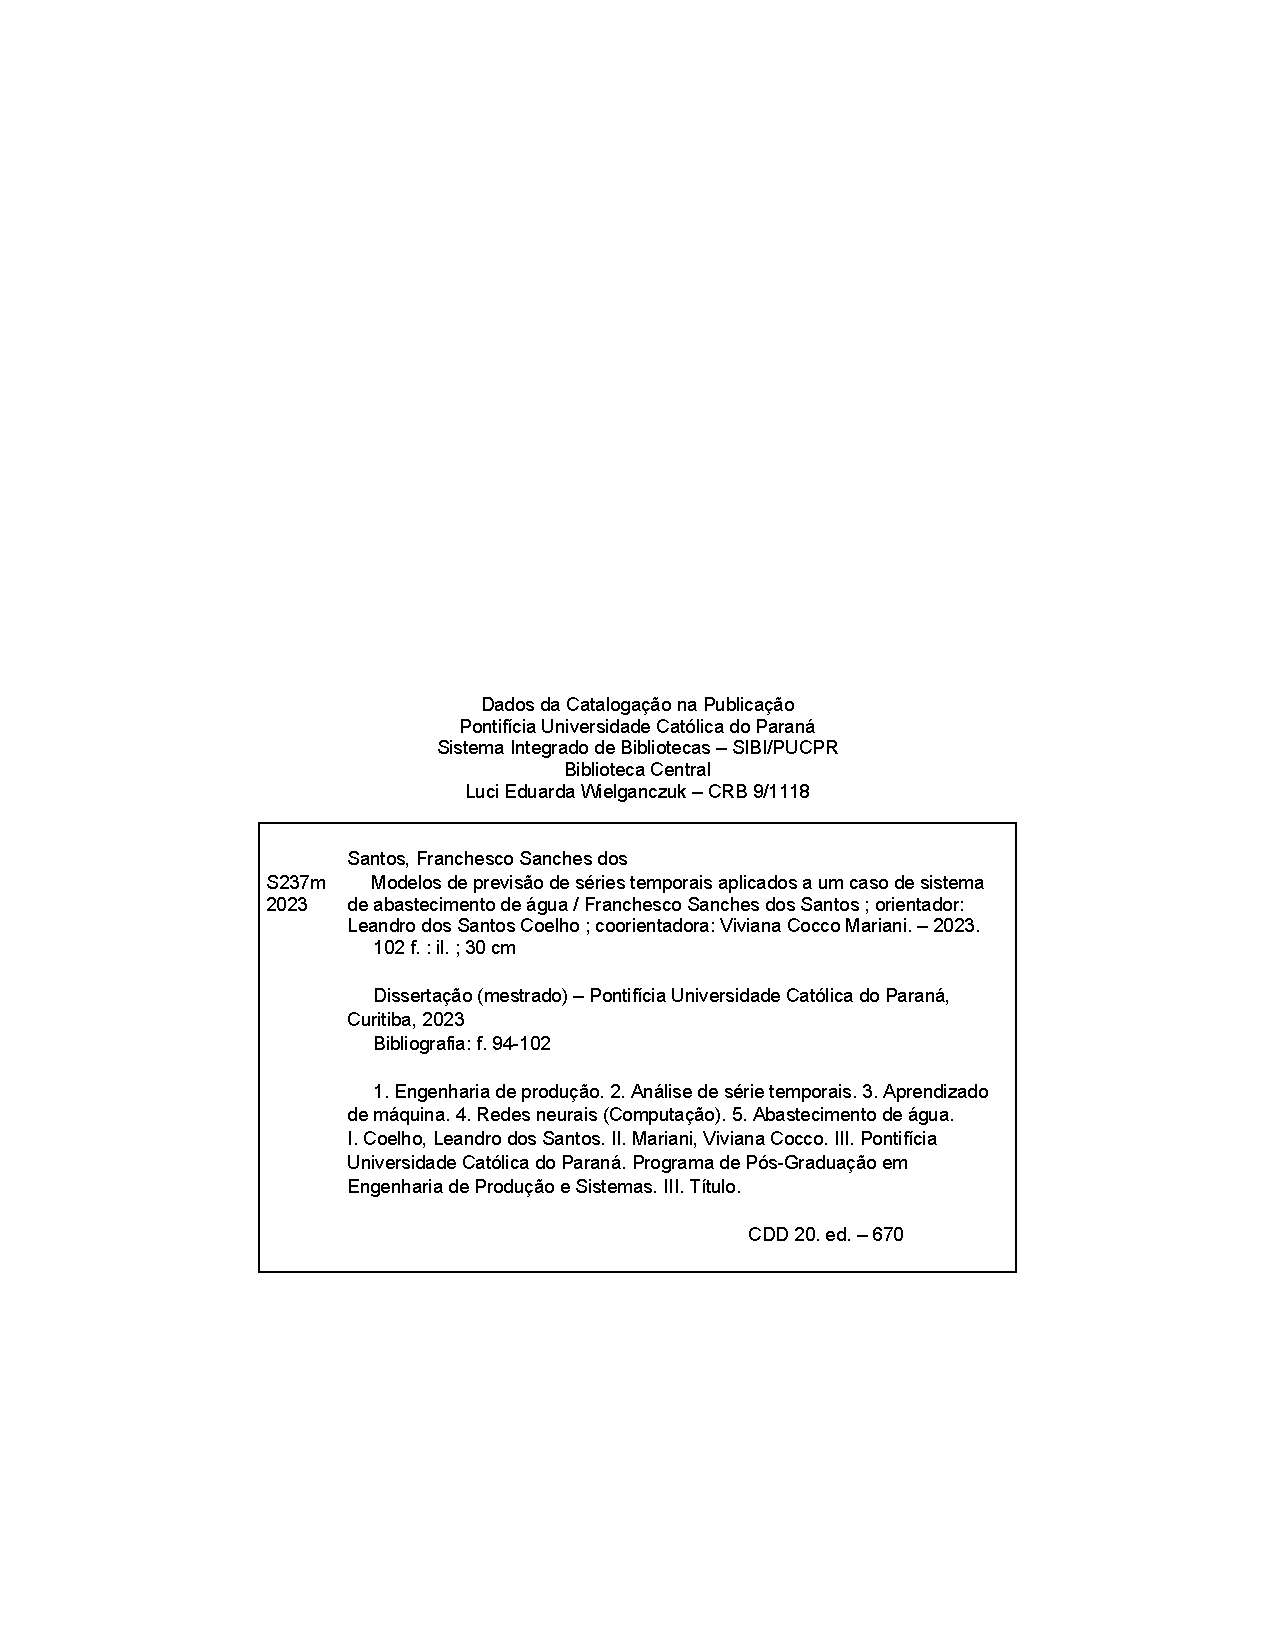
\includepdf{Pretextuais/ficha.pdf}

%% FOLHA DE APROVAÇÃO
\begin{center}
    {\MakeUppercase{\textbf{\aluno}} \\ [1cm]

    \MakeUppercase{\textbf{\titulo}} \\ [1cm]

    \hspace{.45\textwidth} %% POSICIONANDO A MINIPAGE
        \begin{minipage}{.5\textwidth}
        \noindent Dissertação apresentada ao \curso. Área de concentração: Gerência de Produção e Logística, da \departamento, da \universidade, como requisito parcial à obtenção do título de Mestre em Engenharia de Produção e Sistemas. \\ [5mm]
        \end{minipage}
    \textbf{COMISSÃO EXAMINADORA} \\ [5mm]
    
    \rule{5cm}{.1mm} \\ \orientador \\ Orientador\\ \universidade \\ [5mm]

    \rule{5cm}{.1mm} \\ \coorientador \\ Coorientadora \\ \universidade \\ [5mm]

    \rule{5cm}{.1mm} \\ \convidadoa \\ Membro Interno \\ \univconvidadoa \\ [5mm]
    
    \rule{5cm}{.1mm} \\ \convidadob \\ Membro Externo \\ \univconvidadob \\ [5mm]
    

  
    
    \cidade, \datadefesa
    }
\end{center}
 %% NÃO ASSINADA
%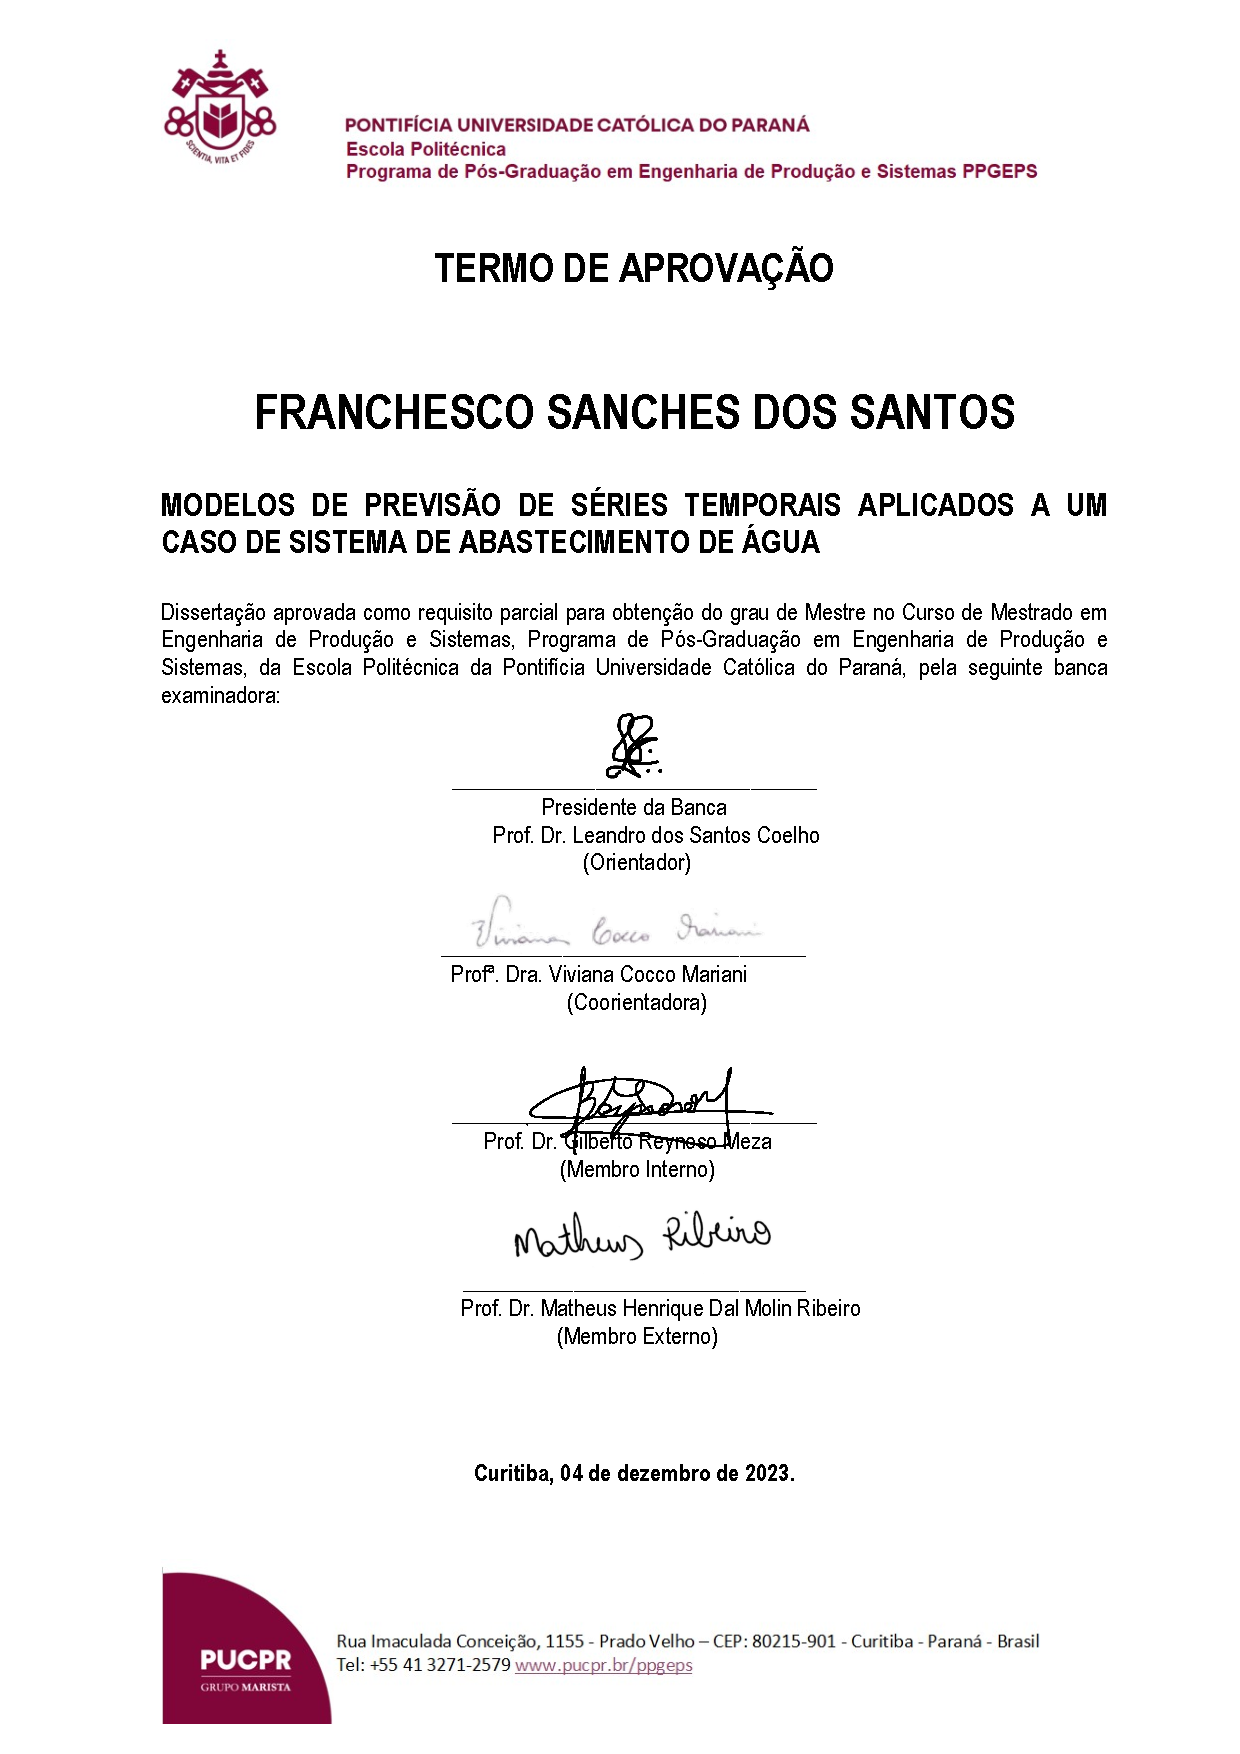
\includepdf{Pretextuais/folha_aprovacao1.pdf} %% ASSINADA

%% DEDICATÓRIA
\vspace*{\fill}

\begin{dedicatoria}
	Dedico essa dissertação de mestrado à Deus, essa força maior, que me guia e ilumina meus pensamentos para que eu desenvolva minha luz.
\end{dedicatoria}


%% AGRADECIMENTOS
\begin{center}
    \textbf{Agradecimentos}
\end{center}

Primeiramente, expresso minha gratidão a Deus por todas as bênçãos recebidas, pois foi Ele quem abriu caminhos e me deu forças para superar esse desafio, tornando-o possível.

À minha família, sou grato pelo apoio incondicional e pelo estímulo constante para seguir em frente com determinação, buscando sempre alcançar novos patamares.

Agradeço ao professor Leandro dos Santos Coelho pela oportunidade de trabalhar ao seu lado e compartilhar seus conhecimentos e experiências ao longo do meu mestrado. Sua orientação contribuiu significativamente para o meu crescimento profissional e pessoal, tornando este trabalho uma realidade.

À professora Viviana Cocco Mariani, agradeço pela disponibilidade e paciência em me auxiliar nas minhas dificuldades, utilizando seu conhecimento para contribuir com o desenvolvimento da pesquisa.

Quero expressar minha gratidão à equipe da Pontifícia Universidade Católica do Paraná (PUCPR) e aos demais professores, especialmente à secretária Denise da Mata Medeiros (PPGEPS), pela paciência, carinho e apoio prestados em diversas ocasiões, sem medir esforços.

Aos meus amigos, que sempre torceram por mim, e aos novos amigos que conquistei ao longo dessa jornada, agradeço por compartilharmos momentos de alegria nessa batalha.

Sou grato ao investimento em bolsas de estudo concedidas pela Coordenação de Aperfeiçoamento de Pessoal de Nível Superior (CAPES), que possibilitou a conclusão dessa etapa da minha carreira profissional e acadêmica.



%% EPÍGRAFE
\begin{center}
\vspace*{\fill}
\hspace{.45\textwidth} %% POSICIONANDO A MINIPAGE
    \begin{minipage}{.5\textwidth}
    \flushright
    \noindent \textit{``A matemática é o alfabeto no qual Deus escreveu o universo.''}
    
    Galileu Galilei
    \end{minipage}
\end{center}


%% RESUMO
\begin{abstract} 
	\noindent Este estudo explora a importância da previsão de séries temporais para a tomada de decisões relacionadas à demanda de água, visando um controle eficaz dos recursos hídricos em um ambiente competitivo. O desafio reside na obtenção de séries temporais confiáveis que auxiliem nas decisões sobre o fornecimento de água. A abordagem proposta envolve a utilização de modelos de previsão de séries temporais para melhorar a precisão das estimativas de demanda.
	Existem várias abordagens discutidas na literatura para a análise e previsão de séries temporais no campo do abastecimento de água. Neste estudo, o caso da SANEPAR (Companhia de Saneamento do Paraná) é examinado como exemplo representativo. No entanto, o que torna este estudo único é a introdução e avaliação personalizada de modelos de redes neurais, como GRU (do inglês \textit{Gated Recurrent Unit}), LSTM (do inglês \textit{Long Short-Term Memory}), RNN (do inglês \textit{Recurrent Neural Network}) e Transformer na forma personalizada para esse problema, além do modelo do Facebook Prophet, que não foram aplicados a esse contexto até então. A técnica de regressão em árvore de decisão também é explorada. Esses métodos inovadores expandem as possibilidades na previsão da demanda por água.
	Com base nesse conhecimento, métodos e produtos específicos são analisados, levando em consideração fatores externos e sazonalidade, além de usar modelos ARIMA (do inglês \textit{Auto-Regressive Integrated Moving Average}), técnicas de \textit{boosting} como XGBoost (do inglês \textit{eXtreme Gradient Boosting}) e LightGBM (do inglês \textit{Light Gradient Boosting Machine}), regressão linear e RFR (do inglês \textit{Random Forest Regression}). A eficácia dessas abordagens é avaliada por métricas como sMAPE (do inglês \textit{Symmetric Mean Absolute Percentage Error}), MAE (do inglês \textit{Mean Absolute Error}) e RRMSE (do inglês \textit{Root Relative Mean Square Error}), fornecendo informações sobre a capacidade dos modelos de previsão no fornecimento de água.
	Esses resultados são úteis para tomar decisões mais informadas no contexto da empresa SANEPAR. Eles fornecem informações sobre como os modelos de previsão de séries temporais se saem em relação ao abastecimento de água.
	A análise e comparação de todos os casos, ficou evidente que o modelo RNN obteve o menor erro em todas as métricas avaliadas, como SMAPE, MAE e RRMSE. É interessante notar que o desempenho do modelo RNN foi excepcional, com erros de previsão consistentemente abaixo de 1\% em todas as análises. Isso destaca que ele é o modelo mais eficiente e preciso em todas as aplicações avaliadas.

\hspace{1cm}


    \noindent \textbf{Palavras-chave:} Previsão de séries temporais, Economia de água, Séries temporais, Modelos de Previsão.
\end{abstract}



%% ABSTRACT
{\selectlanguage{english}
	\begin{abstract}
		
		
%		\noindent The study, situated in the context of water supply in Curitiba, focuses on the effectiveness of forecasting water demand in Bairro Alto from $2018$ to $2020$. The central question investigated is how to anticipate water demand for more efficient planning in the context of scarcity faced by the residents. The purpose of the work is to contribute to the effective control of water resources, utilizing forecasting models, with an emphasis on improving water supply in a competitive environment.
%		Models such as \textit{Auto-Regressive Integrated Moving Average} (ARIMA), \textit{Decision Tree} (DT), \textit{eXtreme Gradient Boosting} (XGBoost), and \textit{Recurrent Neural Network} (RNN) are explored for time series forecasting, with a comparative analysis of effectiveness. The need for a new or better solution arises from the water scarcity in Bairro Alto, justifying the search for more efficient methods of demand forecasting.
%		The proposed solution involves the application of machine learning models such as ARIMA, DT, XGBoost, and especially RNN in forecasting water demand. The basic methodology includes applying these models to the data collected by SANEPAR (Sanitation Company of Paraná).
%		The features responding to the initial questions are assessed through metrics such as \textit{Symmetric Mean Absolute Percentage Error} (sMAPE), \textit{Mean Absolute Error} (MAE), and \textit{Root Relative Mean Square Error} (RRMSE), highlighting that the RNN model consistently demonstrated the lowest errors in all analyses. It is concluded that the proposed approach significantly contributes to water demand forecasting, providing a more efficient and sustainable planning of water supply in Bairro Alto.
%		

\noindent This study, situated in the context of water supply in Curitiba, exemplifies a comprehensive approach to address the growing challenges of water demand. Focusing specifically on the effectiveness of demand forecasting in Bairro Alto, the primary objective is to ensure that the existing infrastructure can meet the continually growing needs of the population, avoiding issues of inadequate supply. The analysis of time series forecasting models is conducted to provide a precise analysis of water demand prediction.
Utilizing data collected by the Companhia de Saneamento do Paraná during the years $2018$ to $2019$, this study proposes a significant contribution to the effective control of water resources. The emphasis is on a variety of forecasting models, including Auto-Regressive, Auto-Regressive with Exogenous Inputs, Moving Average, Auto-Regressive Moving Average, Seasonal Auto-Regressive Integrated Moving Average , ARIMA with Exogenous Inputs, and Seasonal ARIMA with Exogenous Inputs.
In addition to these models, the study particularly highlights the Recurrent Neural Network (RNN), which consistently demonstrated the smallest errors in all analyses. Exploring forecast horizons of one hour ahead, six hours ahead, twelve hours ahead, and twenty-four hours ahead, the detailed results show the different performances of these models.
For 1-hour ahead forecasts, the RNN achieves a Symmetric Mean Absolute Percentage Error (SMAPE) of $0.1647$, Mean Absolute Error (MAE) of $0.0057$, and Root Relative Mean Square Error (RRMSE) of $0.0022$.
At the 6-hour ahead horizon, the RNN demonstrates an SMAPE of $0.1356$, MAE of $0.0046$, and RRMSE of $0.0022$, highlighting its accuracy in this time interval.
When considering 12-hour ahead forecasts, the RNN achieves an SMAPE of $0.1343$, MAE of $0.0046$, and RRMSE of $0.0021$, indicating its consistency in longer time horizons.
For 24-hour ahead projections, the RNN maintains remarkable performance with an SMAPE of $0.2231$, MAE of $0.0077$, and RRMSE of $0.0028$.
These results underscore the reliability of the RNN in water demand forecasting across different time scales, thereby providing efficient and sustainable water supply planning in the region.

		\hspace{1cm}
		
		\noindent \textbf{Keywords:} Forecasting, Time series, Water supply, Machine learning, Artificial neural networks.
	\end{abstract}
}



%% LISTA DE FIGURAS
\newpage 
\pdfbookmark[1]{\listfigurename}{lof}
\listoffigures 

%% LISTA DE TABELAS
\newpage 
\pdfbookmark[1]{\listtablename}{lot}
\listoftables
\cleardoublepage



%% Lista de abreviaturas e siglas (opcional)

\section*{Lista de Abreviaturas e Siglas}

\begin{tabular}{cp{0.65\textwidth}}
	AdaBoost & Impulso ou Estímulo adaptativo (do inglês \textit{Adaptive Boosting}) \\
	AR & Auto-Regressivo\\
	ARIMA & Média Móvel Integrada Auto-Regressiva (do inglês \textit{autoregressive integrated moving average}) \\
	ARIMAX & Média Móvel Integrada Auto-Regressiva com regressores eXogenous (do inglês \textit{autoregressive integrated moving average with eXogenous regressors})\\
	ARMA & Média Móvel Auto-Regressivo (do inglês \textit{autoregressive moving average}) \\
	ARX & Auto-Regressivo com variável Exógena (do inglês \textit{autoregressive with eXogeneous inputs})\\ 
	BrownBoost & Algoritmo de aumento\\
	CNN & Rede Neural Convolucional (do inglês \textit{Convolutional Neural network ou ConvNet})\\
	DBN & Rede de Crenças Profundas (do inglês \textit{Deep Belief Network}) \\
	EFB & Pacote de características exclusivas (do inglês \textit{Exclusive Feature Bundling})\\
	FT & flow transmitter (Transmissor de fluxo)\\
	Hz & Hertz\\
	INMET & Instituto Nacional de Meteorologia\\
	LGBMRegressor & Regressão Ligth GBM\\
	Light GBM & Máquina de Impulso de Gradiente Leve (do inglês \textit{Light Gradient Boosting Machine}) \\
	LogitBoost & Representa uma aplicação de técnicas de regressão logísticas\\
	LPBoost & Reforço da Programação Linear (do inglês \textit{Linear Programming Boosting}) \\
	LR & Regressão linear (do inglês \textit{Linear Regression})\\
	LSTM & Memória de longo curto prazo (do inglês \textit{Long short-term memory})\\
	$m^3$  & Metros cúbicos\\
	$m^3/h$ & Metros cúbicos por hora	
\end{tabular}

\begin{tabular}{cp{0.65\textwidth}}
	MA & Média Móvel (do inglês \textit{moving average})\\
	MadaBoost & Modificando o sistema de ponderação da AdaBoost\\
	MAE & Erro Médio Absoluto (do inglês \textit{Mean Absolute Error})\\
	MAPE & Erro Percentual Médio Absoluto (do inglês \textit{Mean Absolute Percentage Error})\\
	mca & Metros coluna de água\\
	ML & Aprendizado de máquina (do inglês \textit{machine learning})\\
	mm & Milímetros\\
	MSE & Erro médio quadrático (do inglês \textit{Mean Squared Error})\\
	PR & Estado do Paraná\\
	RBAL & Recalque Bairro Alto\\
	RFR & Regressão de floresta aleatória (do inglês \textit{Random Forest Regression})\\
	RMSE & Erro de Raiz Média Quadrática (do inglês \textit{Root Mean Squared Error})\\
	RNN & Rede Neural Recorrente (do inglês \textit{Recurrent Neural Network})\\
	SANEPAR & Companhia de Saneamento do Paraná \\
	SARIMA & Auto-Regressivos Integrados de Médias Móveis com Sazonalidade (do inglês \textit{Integrated Auto-Regressive Moving Averages with Seasonality}) \\
	SARIMAX &  Média Móvel Integrada Auto-Regressiva Sazonal com regressores eXogenous (do inglês \textit{Seasonal Auto-Regressive Integrated Moving Average with eXogenous regressors}) \\
	SVM-VAR & Máquinas de vetor de suporte - Vetores Auto-Regressivos\\
	Totalboost & Impulso total\\
	XGBoost & Impulso Gradiente Extremo (do inglês \textit{eXtreme Gradient Boosting})\\
	XGBRegressor & Regressão XGBoost
\end{tabular}




\nomenclature{ABNT}{Associação Brasileira de Normas Técnicas}
\nomenclature{LaTeX}{Sistema de preparação de documentos}
\nomenclature{HTML}{Hypertext Markup Language}

%\sym{ABNT}{Associação Brasileira de Normas Técnicas}


%% SUMÁRIO
\newpage
\pdfbookmark[1]{\contentsname}{toc}
\tableofcontents 

%-----------------------------------------------------------------
%% ELEMENTOS TEXTUAIS

%% INTRODUÇÃO
\setlength{\parskip}{1pt} %% ESPAÇO DEPOIS DE 6pt
\pagenumbering{arabic}  %% PAGINAÇÃO INICIA AQUI
\setcounter{page}{16} % Reiniciar contagem de página para 1
%\pagestyle{plain} % Restaurar numeração de página com estilo "plain"
\clearpage
\pagestyle{fancy}


\section{Introdu{\c c}{\~a}o} \label{sec:int}

Este capítulo apresenta o que é abordado nesta dissertação utilizando modelos ML dentro destes modelos será abordado a previsão futura dos dados coletados na SANEPAR, estes dados foram coletados no bairro alto nos anos de 2018 a 2020 houve uma falta de abastecimento de água que afetou a todos na capital paranaense.

No uso do pensamento de séries temporais nesse contexto de tomada de decisão, pode-se pensar em aplicar modelos de ML a séries temporais usando os modelos mais clássicos encontrados durante uma revisão sistemática do conteúdo para tabular alguns modelos usados na literatura.  



\subsection{Contexto da pesquisa} \label{subsec:contexto}
\citeonline{mateus} A necessidade de desenvolvimento do planejamento estratégico no mundo corporativo e no dia-a-dia torna a análise de séries temporais e previsões valiosas ferramentas para apoiar o processo de tomada de decisão a curto, médio e longo prazo. Devido a não linearidades, sazonalidade, tendência e ciclicidade nos dados temporais, o desenvolvimento de modelos de previsão eficientes é uma tarefa desafiadora. 

 Em séries temporais, o aprendizado de máquina é frequentemente utilizado para processamento de big data, com o conjunto de dados da SANEPAR em Curitiba - PR, na cidade há algum consumo e escassez de água, é necessário avaliar os dados para ter certeza do que está acontecendo, quando há escassez d'água, e picos que ocorrem entre horas e dias.
 
 Dentre os modelos preditivos que serão apresentados em uma revisão sistemática, avaliar o melhor modelo que podemos utilizar e validar quando e como ocorre a escassez d'água. Estas análises será em \textit{python}.
 
 Explorar o que são séries temporais e aprendizado de máquina, séries temporais são dados armazenados ao longo do tempo que permitem ao observador analisar anomalias nos dados. Em séries temporais, ordenar os dados por ano ou dia é fundamental e, se os dados atribuídos de forma aleatória, assim podendo tornar mais difícil prever e tomar decisão baseado nos dados coletados. 
 Analisar médias pode ser bem perigoso se não excluir pontos fora da curva também conhecidos como \textit{outliers}. Pode gerar dados muito positivos ou negativos que não correspondem a realidade.
   
      
\subsubsection{Motiva\c c\~ao da pesquisa} \label{subsubsec:motivacao}
   %Escrever algo motivador 
    
    De acordo com \cite{vasconcelos_2020} Curitiba e região metropolitana enfrentou um rodízio com $36$ horas com água e $36$ horas sem abastecimento. A média geral dos reservatórios da região está em $27,96\%$ da capacidade. Assim em medida a isso essa pesquisa tem como a abordagem da falta de água, essa falta que pode ser vista como uma seca, em média nos anos anteriores de 2020 a chuva tem marcado a quantia de $1.704$ mm. \cite{vasconcelos_2020} Desde 2016, quando registrou 1.704 mm de chuva, Curitiba não atingiu mais a média anual de precipitação, que é de 1.490 mm, com base em dados da estação pluviométrica do Instituto Nacional de Meteorologia (Inmet).  Apesar de abaixo da média, o mínimo registrado desde então ocorreu em 2020, com 1.158 mm.
    
    Em mediano a essa motivação pode ser melhor interpretado os dados que a SANPEAR ofertor para prever e evitar a escasseia de água que foi registada, e a anomalia que foi detectado em 2020, com a volta da chuva os reservatórios teve aumento do nível.
    
          
\subsection{Objetivo Geral} \label{subsec:objetivos}

O objetivo desta pesquisa é identificar o modelo de aprendizado de máquina mais adequado para previsão de séries temporais. 

Ao longo da dissertação, serão avaliados diversos modelos de regressão, com destaque para os modelos de redes neurais e o Prophet. É importante mencionar que a pesquisa enfatizará os modelos de \textit{gradient boosting}, além do ARIMA e suas variações mais contemporâneas. Além das previsões, também serão realizadas análises de anomalias nos dados, buscando compreender as causas subjacentes a essas ocorrências.
 
    
    
    \subsubsection{Objetivos Espec\'ificos e Quest\~ao de Pesquisa} \label{subsubsec:obespec}
    
Neste estudo, busca-se identificar e compreender possíveis anomalias nos dados, bem como investigar as causas por trás dessas ocorrências. Entre os objetivos específicos está responder às perguntas de pesquisa relacionadas a essas anomalias.

\begin{enumerate}[start=1, label={\textbf{Q} \arabic*}]
	\item \label{q1} Qual é a adequação da pressão atual para atender à demanda diária?
	\item \label{q2} Qual é o volume mínimo de água necessário no reservatório para evitar o acionamento das bombas durante o horário de pico? 
	\item \label{q3} Qual é a vazão ótima para atender à demanda diária?
	\item \label{q4} Como encontrar o ponto de equilíbrio entre a demanda e a vazão?
	\item \label{q5} Qual é o impacto do acionamento das bombas durante o horário de pico?
	 
	\begin{enumerate}[label=\alph*.]
	\item \label{q5:a} Qual é o nível ideal no reservatório para evitar a ativação das bombas da SANEPAR durante o período de maior demanda, das 18h às 21h, sem comprometer o abastecimento de água para a população?  
	\item \label{q5:b} Existe tendência, padrão, sazonalidade para os dados destes três anos do Bairro Alto?
	\item \label{q5:c} Identificar quais os horários de maior demanda das $18$ às $21$?
	\item \label{q5:d} Quanto deve-se armazenar previamente no reservatório para não acionar as bombas no horário de pico?
	\item \label{q5:e} Se a vazão cresce e a pressão decresce existe uma ANOMALIA na rede (com base no histórico).	
	\end{enumerate}
\end{enumerate}

   
\subsection{Descri\c c\~ao do problema} \label{subsec:descricao}

A descrição do problema é fundamental para obter uma compreensão mais precisa do que está sendo abordado neste trabalho. É por meio dessa descrição que as variáveis-chave são expostas e o objetivo da previsão é estabelecido de forma clara. Sem um plano estruturado para determinar o que deve ser previsto, torna-se difícil justificar o uso de modelos de previsão de dados. Portanto, é essencial estabelecer um propósito claro e definir as metas da previsão antes de aplicar os modelos adequados.

\begin{itemize}
	\item Bombas de sucção (B1, B2 e B3) – valor máximo da frequência 60 Hz
	
	\item[] Variáveis importantes: Fluxo, pressão e nível
	
	\item Nível do Reservatório (Câmara 1) LT01 $ (m^3) $ - \textbf{PREVER}
	
	\item Vazão de entrada (FT01) $ (m^3/h) $
	
	\item Vazão de gravidade (FT02) $ (m^3/h) $
	
	\item Vazão de recalque (FT03) $ (m^3/h) $
	
	\item Pressão de Sucção (PT01SU) (mca)
	
	\item Pressão de Recalque (PT02RBAL) (mca)
\end{itemize}

A pesquisa fará uso da variável LT01, que representa o nível do reservatório e desempenha um papel de extrema importância, como evidenciado pelas Figuras \ref{fig:dados-todos} e \ref{fig:2020-a-frente}. Essas figuras retratam as anomalias ocorridas durante o período em que a capital paranaense foi afetada pela escassez de chuvas, resultando na redução do nível dos reservatórios e na implementação de rodízios periódicos, conforme discutido na subseção \ref{subsubsec:motivacao}. Assim, tais observações permitem uma compreensão mais aprofundada das perspectivas futuras.

\subsection{Procedimentos metodol{\'o}gicos} \label{subsec:metod}

Com o intuito de realizar previsões e fazer comparações entre os modelos obtidos na revisão sistemática, será adotado um processo metodológico bem definido. Tal processo está detalhado na subseção \ref{subsubsec:etp} desta seção, onde foram estabelecidas as etapas a serem seguidas desde o início. Isso inclui a definição do que será previsto, bem como a seleção dos métodos a serem utilizados na Análise Exploratória de Dados (EDA), seguindo uma sequência lógica e coerente.
   
    \subsubsection{Etapas da pesquisa}\label{subsubsec:etp}

    
    A pesquisa seguiu as seguintes etapas:
    \begin{figure}[H]
    	\centering
    	\caption{Mapa das Etapas}
    	\label{fig:etapas}
    	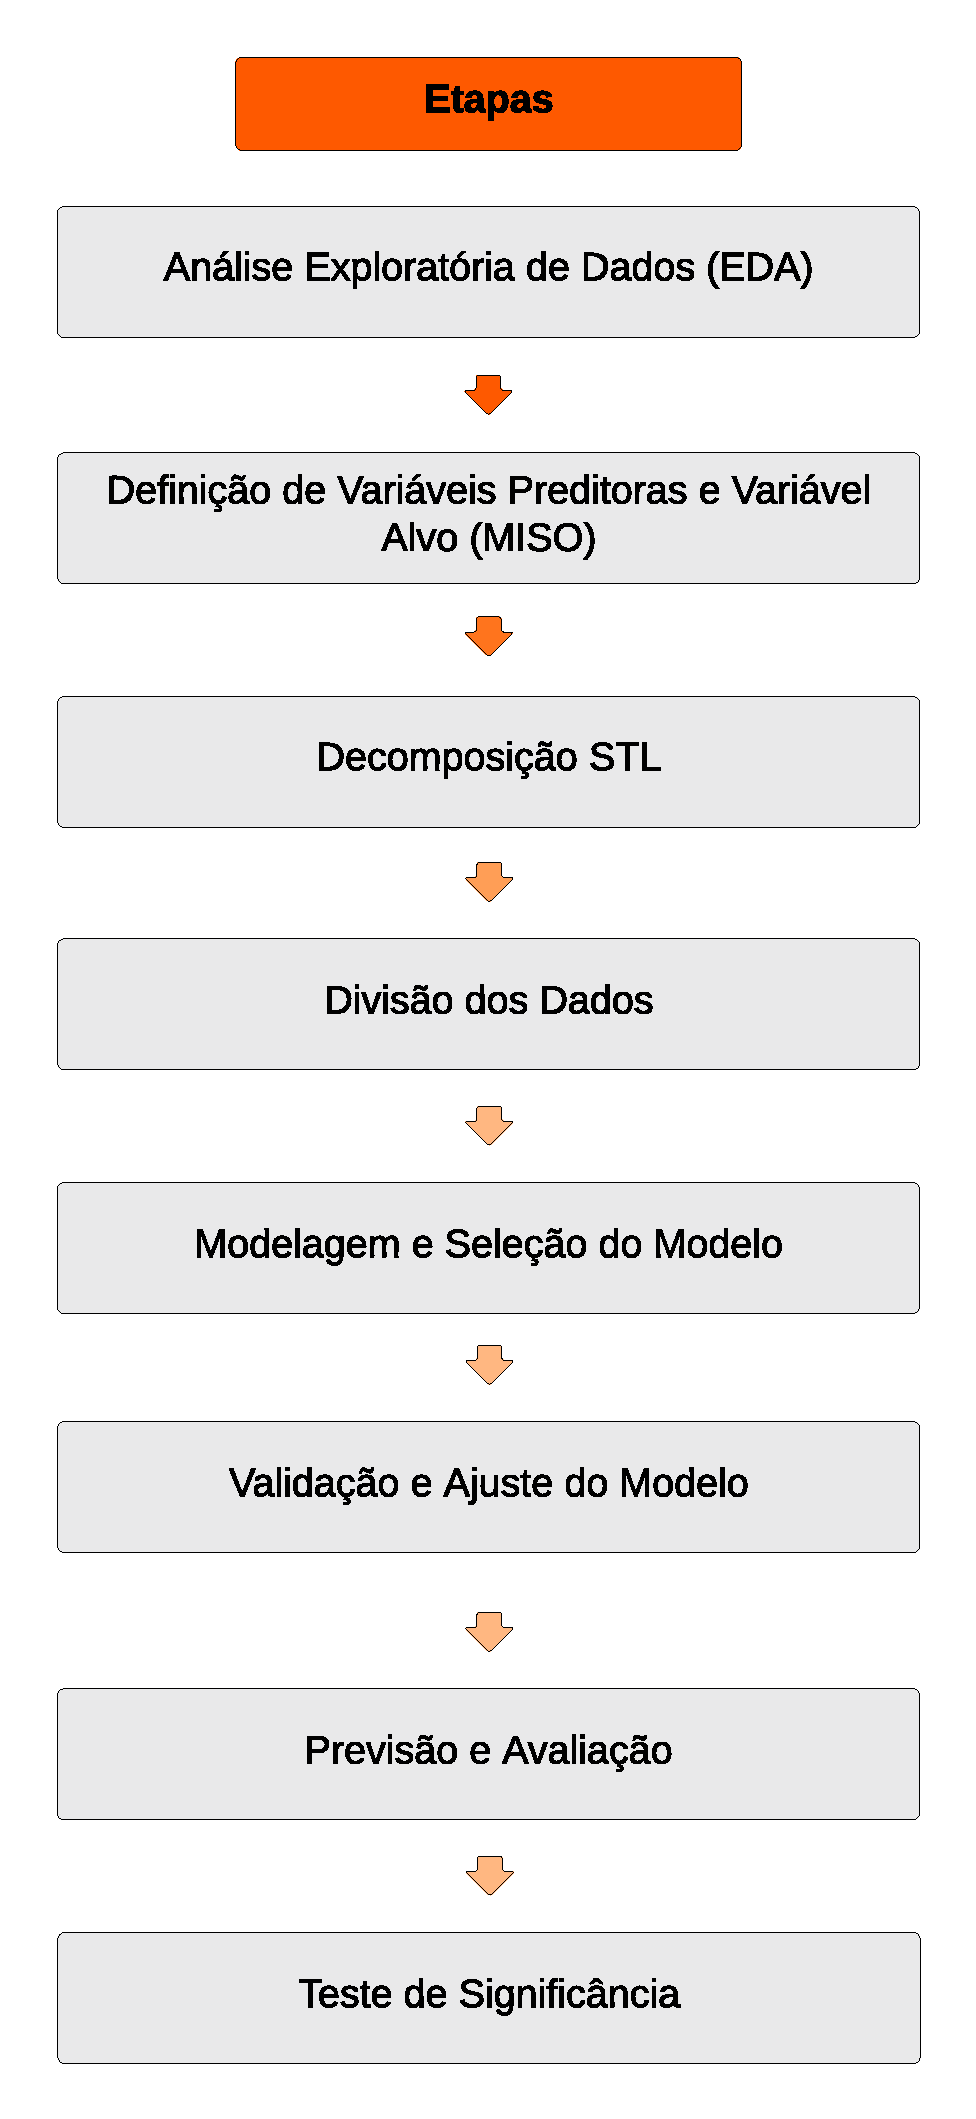
\includegraphics[width=1\linewidth]{Introducao/Figuras/Etapas}
    	
    	\fonte{Elaboração própria}
    \end{figure}
    \begin{enumerate}[start=1, label = {\textbf{Etapa} \arabic*} ]
    	\item Análise exploratória dos dados – EDA ( do inglês \textit{Exploratory Data Analysis}). \label{etp:1}
    	
    	A exploração de dados na EDA é fundamental para entender melhor os dados que estão sendo trabalhados, como, por exemplo, excluir valores ausentes, saber como os dados estão separados em horas ou dias e, assim, tomar a melhor decisão a ser trabalhada com os dados, usar gráficos de linha na análise para observar a convergência dos dados e as anomalias que podem ocorrer.
    	
        	
    	\item O que vai ser usado como variáveis previsoras e qual será a variável a ser predita (MISO). \label{etp:2}
    	
    	Nessa etapa, tem o papel de relacionar as variáveis ao que será previsto, como os modelos de variáveis exógenas que são usados aqui nos modelos SARIMAX, ARX e ARIMAX do tipo ARIMA. Cada modelo tem a interação de mais variáveis do que o modelo ARIMA básico ou seus derivados AR, MA e SARIMA. O conhecimento de quais variáveis estão incluídas na modelagem do problema torna a modelagem mais abrangente quando o horizonte de previsão é estendido além dos dados.
    	
       	
    	\item Fazer a decomposição STL (do inglês \textit{Seasonal-Trend Decomposition}) Sazonalidade, Tendência e Resíduo. \label{etp:3}
    	
    	\citeonline{en15165875} destacam que ``o uso do método de decomposição STL em conjunto com um modelo híbrido se mostrou eficaz na previsão de carga de curto prazo'' (p. 6).
    	
    	Segundo \citeonline{inproceedings}, ``a aplicação da decomposição STL e do modelo LSTM baseado em atenção foi capaz de prever com precisão a velocidade do tráfego de curto prazo'' (p. 6).
    	
    	\citeonline{su13041694} afirmam que ``a combinação da decomposição STL e modelos de aprendizado profundo mostrou-se promissora na previsão de carga de eletricidade'' (p. 18).
    	
        O algoritmo STL executa suavização na série de tempo usando LOESS em dois loops; o loop interno itera entre a suavização sazonal e de tendência e o loop externo minimiza o efeito de valores atípicos. Durante o loop interno, o componente sazonal é calculado primeiro e removido para calcular o componente de tendência. O restante é calculado subtraindo os componentes sazonais e de tendência da série de tempo.
        
        Os três componentes da análise STL se relacionam com a série de tempo bruta da seguinte forma:
        
        \begin{align}
        	y_i &= s_i + t_i + r_i\label{eq:stl1}
        \end{align}
    	
    	Da equação \eqref{eq:stl1}:
    	
    	\begin{itemize}
    		\item $y_i = O$ valor da série de tempo no ponto $i$.
    		\item $s_i = O$ valor do componente sazonal no ponto $i$.
    		\item $t_i = O$ valor do componente de tendência no ponto $i$.
    		\item $ri = O$ valor do componente restante no ponto $i$.
    	\end{itemize}
    	\item \label{etp:4} Separação dos dados.
    	
  
    De acordo com a literatura acadêmica, é comum dividir o conjunto de dados em treinamento, validação e teste para avaliar a performance dos modelos. Essa abordagem permite uma análise mais completa do desempenho do modelo, garantindo uma avaliação objetiva de sua capacidade de generalização e evitando problemas de overfitting ou subajuste \cite{cruz-ramirez2020enhancing,mokhtari2020deep,khan2021hybrid,sharma2021deep}.
    
    A fim de obter uma divisão mais adequada dos dados, é realizado um estudo das medidas de tendência central e dispersão de cada conjunto. O conjunto de dados é então dividido em três partes distintas: treinamento, validação e teste. Nessa divisão, inicialmente, 70\% dos dados são utilizados para o treinamento e validação, enquanto os 30\% restantes são reservados para o conjunto de teste. Em seguida, a porção destinada ao treinamento e validação é subdividida em uma proporção de 80\% para treinamento e 20\% para validação.
    	
    	
    	\item Estratégia de previsão (recursiva e iterada-método direto). \label{etp:5}
    	
    	A estratégia recursiva é mencionada por \citeonline{PETROPOULOS2022705} como uma abordagem eficaz na previsão de séries temporais de múltiplos passos. De acordo com o autor, essa estratégia envolve o uso de previsões anteriores como entradas para prever os próximos passos da série temporal. A abordagem recursiva tem demonstrado potencial para melhorar a acurácia das previsões de séries temporais de longo prazo.
    	
    	A estratégia recursiva consiste em utilizar um modelo de previsão de um passo de tempo várias vezes, onde a previsão obtida no passo anterior é utilizada como entrada para realizar a previsão do próximo passo de tempo.
    	
    	No contexto da previsão da demanda de água para os próximos dias, seria desenvolvido um modelo de previsão de um único passo. Esse modelo seria aplicado para prever a demanda no primeiro dia e, em seguida, essa previsão seria utilizada como dado de entrada para prever a demanda do segundo dia. Esse processo se repetiria para os demais dias, permitindo a previsão da demanda ao longo do tempo.
    	    		 
    	Por Exemplo:
    	
    	\begin{eqnarray}
    	preditivo(t+1) &=& model_1(obs(t-1), obs(t-2), \ldots, obs(t-n))\\
    	preditivo(t+2) &=& model_2(obs(t-2), obs(t-3), \ldots, obs(t-n))   	
    	\end{eqnarray}
    	
    	\citeonline{machinemaster} como as previsões são usadas no lugar das observações, a estratégia recursiva permite que os erros de previsão se acumulem de tal forma que o desempenho possa se degradar rapidamente à medida que o horizonte de tempo de previsão aumenta.
    	
    	
    	\item Horizonte de previsão (1 passo ou n passos à frente). \label{etp:6}
    	
    	Para abordar a diversidade de horizontes de previsão, optou-se por considerar diferentes intervalos de tempo. Isso permitirá a realização de previsões para um passo à frente, uma semana, duas semanas e um mês, de forma a abranger distintas perspectivas de curto e médio prazo. Essa abordagem proporciona uma análise abrangente da capacidade dos modelos em lidar com horizontes de previsão variados, contribuindo para uma avaliação mais completa e precisa do desempenho dos mesmos.
    	
    	
    	\item Modelos de previsão e métricas de desempenho. \label{etp:7}
    	
    	Os modelos abordados nesta pesquisa são tanto os modelos clássicos de previsão quanto os modelos de regressão por gradiente. Entre os modelos clássicos, incluem-se o AR, ARX, ARMA, ARIMA, SARIMA, SARIMAX e ARIMAX, enquanto os modelos de regressão por gradiente englobam o LR, XGBRegressor, RFR e LGBMRegressor. A seleção desses modelos foi baseada em uma revisão sistemática realizada durante a dissertação, buscando identificar os modelos mais eficazes e amplamente utilizados na literatura.
    	
    	Ao longo da pesquisa, foram adotadas três métricas principais para avaliar o desempenho dos modelos: RRMSE, MAE  e sMAPE. Essas métricas foram escolhidas com base na revisão sistemática e são amplamente reconhecidas como medidas de qualidade de previsão. Cada métrica tem sua própria interpretação e importância, sendo detalhada na subseção \ref{subsec:metrica} para um melhor entendimento de como são aplicadas e interpretadas na pesquisa.
    	
    	
    	
    	%\item Ajustar os hiperparâmetros dos modelos de previsão Hiperparâmetro ajusta a priori (ex: número de neurônios da rede neural), e parâmetro (pesos da rede neural) ajusta durante o processo. \label{etp:8}
    	
    	
    	\item Aplicar os modelos de previsão e fazer comparativo baseado em testes de significância estatística (\textit{Friedman e Nemenyi}). \label{etp:9}
    	
    	
    	O teste de Friedman é o teste não paramétrico usado para comparar dados de amostras vinculadas, ou seja, quando o mesmo indivíduo é avaliado mais de uma vez. 
    	ou seja, quando o mesmo indivíduo é avaliado mais de uma vez. 
    	O teste de Friedman não usa os dados numéricos diretamente, mas sim as classificações ocupadas pelos dados após a classificação de cada grupo separadamente. 
    	separadamente. Após a classificação, a hipótese de igualdade da soma das classificações de cada grupo é testada. 

		O teste consiste em fazer comparações em pares com o intuito de verificar qual dos fatores que diferem entre si. No entanto, o teste de Nemenyi é muito conservador e pode não encontrar diferença significativa entre os pares testados.
    	
    \end{enumerate}






    
    
\subsection{Justificativa da Pesquisa} \label{subsec:justif}

Ao longo desta dissertação, os seguintes aspectos são abordados visando a previsão e tomada de decisões.

\subsubsection{Contribui\c c\~oes} \label{subsubsec:Contribuição}

As perguntas de pesquisa apresentadas na subseção \ref{subsubsec:obespec}, surgem duas contribuições significativas nesta dissertação. A primeira diz respeito à previsão da demanda de água na cidade de Curitiba, abordando aspectos como consumo e gasto de energia durante períodos de pico.

Segundo estudos recentes, os modelos ARIMA desempenham um papel fundamental na análise de séries temporais. Os modelos ARIMA são utilizados na previsão de séries temporais devido à sua capacidade de capturar padrões complexos e comportamentos de longo prazo \cite{arima_python}.

Conforme relatos, o modelo XGBoost tem sido aplicado com sucesso em problemas de previsão de séries temporais. Estudos demonstraram que o XGBoost é uma ferramenta para lidar com desafios de previsão em séries temporais \cite{xgboost_intro}. O LightGBM tem ganhado destaque como um modelo eficiente para previsão de séries temporais \cite{WELLENS20221482}. De acordo com \citeonline{decisiontree}, o algoritmo de árvore de decisão é um dos mais populares e eficazes na área de classificação. Alguns modelos baseados em árvores possuem eficiência computacional e são capazes de lidar tanto com dados categóricos quanto numéricos. Já \citeonline{random_forest_regression} enfatiza a importância do uso de \textit{Random Forest Regression} na previsão de séries temporais.

As RNNs (Redes Neurais Recorrentes) são redes neurais artificiais que possibilitam o processamento de dados sequenciais. Elas são amplamente utilizadas em mineração de dados e aprendizado de máquina devido à sua habilidade em modelar dependências temporais \cite{rnn}. Assim como outras redes neurais artificiais, as RNNs são capazes de lidar com a detecção de anomalias de forma mais eficaz do que modelos mais básicos de séries temporais, como o modelo ARIMA e seus predecessores. Enquanto o ARIMA pode identificar anomalias nos dados, as RNNs podem ajustar e otimizar os neurônios para aumentar a eficácia na detecção dessas anomalias.

As CNNs (Redes Neurais Convolucionais) representam uma classe de redes neurais profundas amplamente utilizadas em tarefas de reconhecimento de imagens e vídeos \cite{cnn}. Embora sejam uma opção vantajosa para previsões de tempo, assim como as RNNs, as CNNs são especialistas em dados bidimensionais. Isso pode resultar em erros maiores quando comparadas às RNNs em contextos de dados sequenciais.

As GRUs (Unidades Recorrentes com Portões)  são um tipo de rede neural recorrente introduzido como alternativa às LSTMs (Unidades de Memória de Longo e Curto Prazo) \cite{gru}. As LSTMs, por sua vez, foram desenvolvidas para resolver o problema do gradiente desvanecido em RNNs padrão \cite{lstm}. Embora sejam semelhantes às RNNs, as GRUs e LSTMs incorporam técnicas específicas para melhorar a capacidade das RNNs em lidar com dependências temporais a longo prazo. Cada uma delas possui particularidades que as tornam mais adequadas para diferentes cenários de previsão, com a GRU sendo especialmente útil para resolver problemas relacionados à dissipação de gradientes.


Constata-se que as redes GRU demonstram uma vantagem em relação às redes LSTM em termos de complexidade e desempenho. As RNN, incluindo tanto GRU quanto LSTM, são observadas como tendo uma capacidade competitiva em tarefas de aprendizagem de sequências. Portanto, os resultados sugerem que as redes GRU, pertencentes à categoria de RNN, são mais adequadas para a aprendizagem de sequências simbólicas que exigem memória seletiva e adaptativa \cite{DBLP:journals/corr/abs-2107-02248}.

No entanto, de acordo com as constatações dessa pesquisa, o modelo RNN especificamente o GRU é identificado como o melhor modelo para a tarefa em questão. Isso se baseia na habilidade do GRU em eficientemente memorizar e generalizar sequências, resultando em um desempenho superior em comparação a outros modelos, incluindo ANN (do inglês \textit{Artificial Neural Network}), CNN e modelos baseados em gradientes, tais como XGBoost e LightGBM. Dessa forma, conclui-se que o modelo RNN, e mais especificamente o GRU, se destaca como a escolha mais apropriada para a aprendizagem e previsão de séries temporais.



    
\subsection{Estrutura do trabalho} \label{subsec:estrutura}

 Este documento está estruturado em~\ref{sec:conclusoes} capítulos, divididos da seguinte forma:
   
    \begin{figure}[H]
    	\centering
    	\caption{Estrutura da dissertação}
    	\label{fig:estrutura}
    	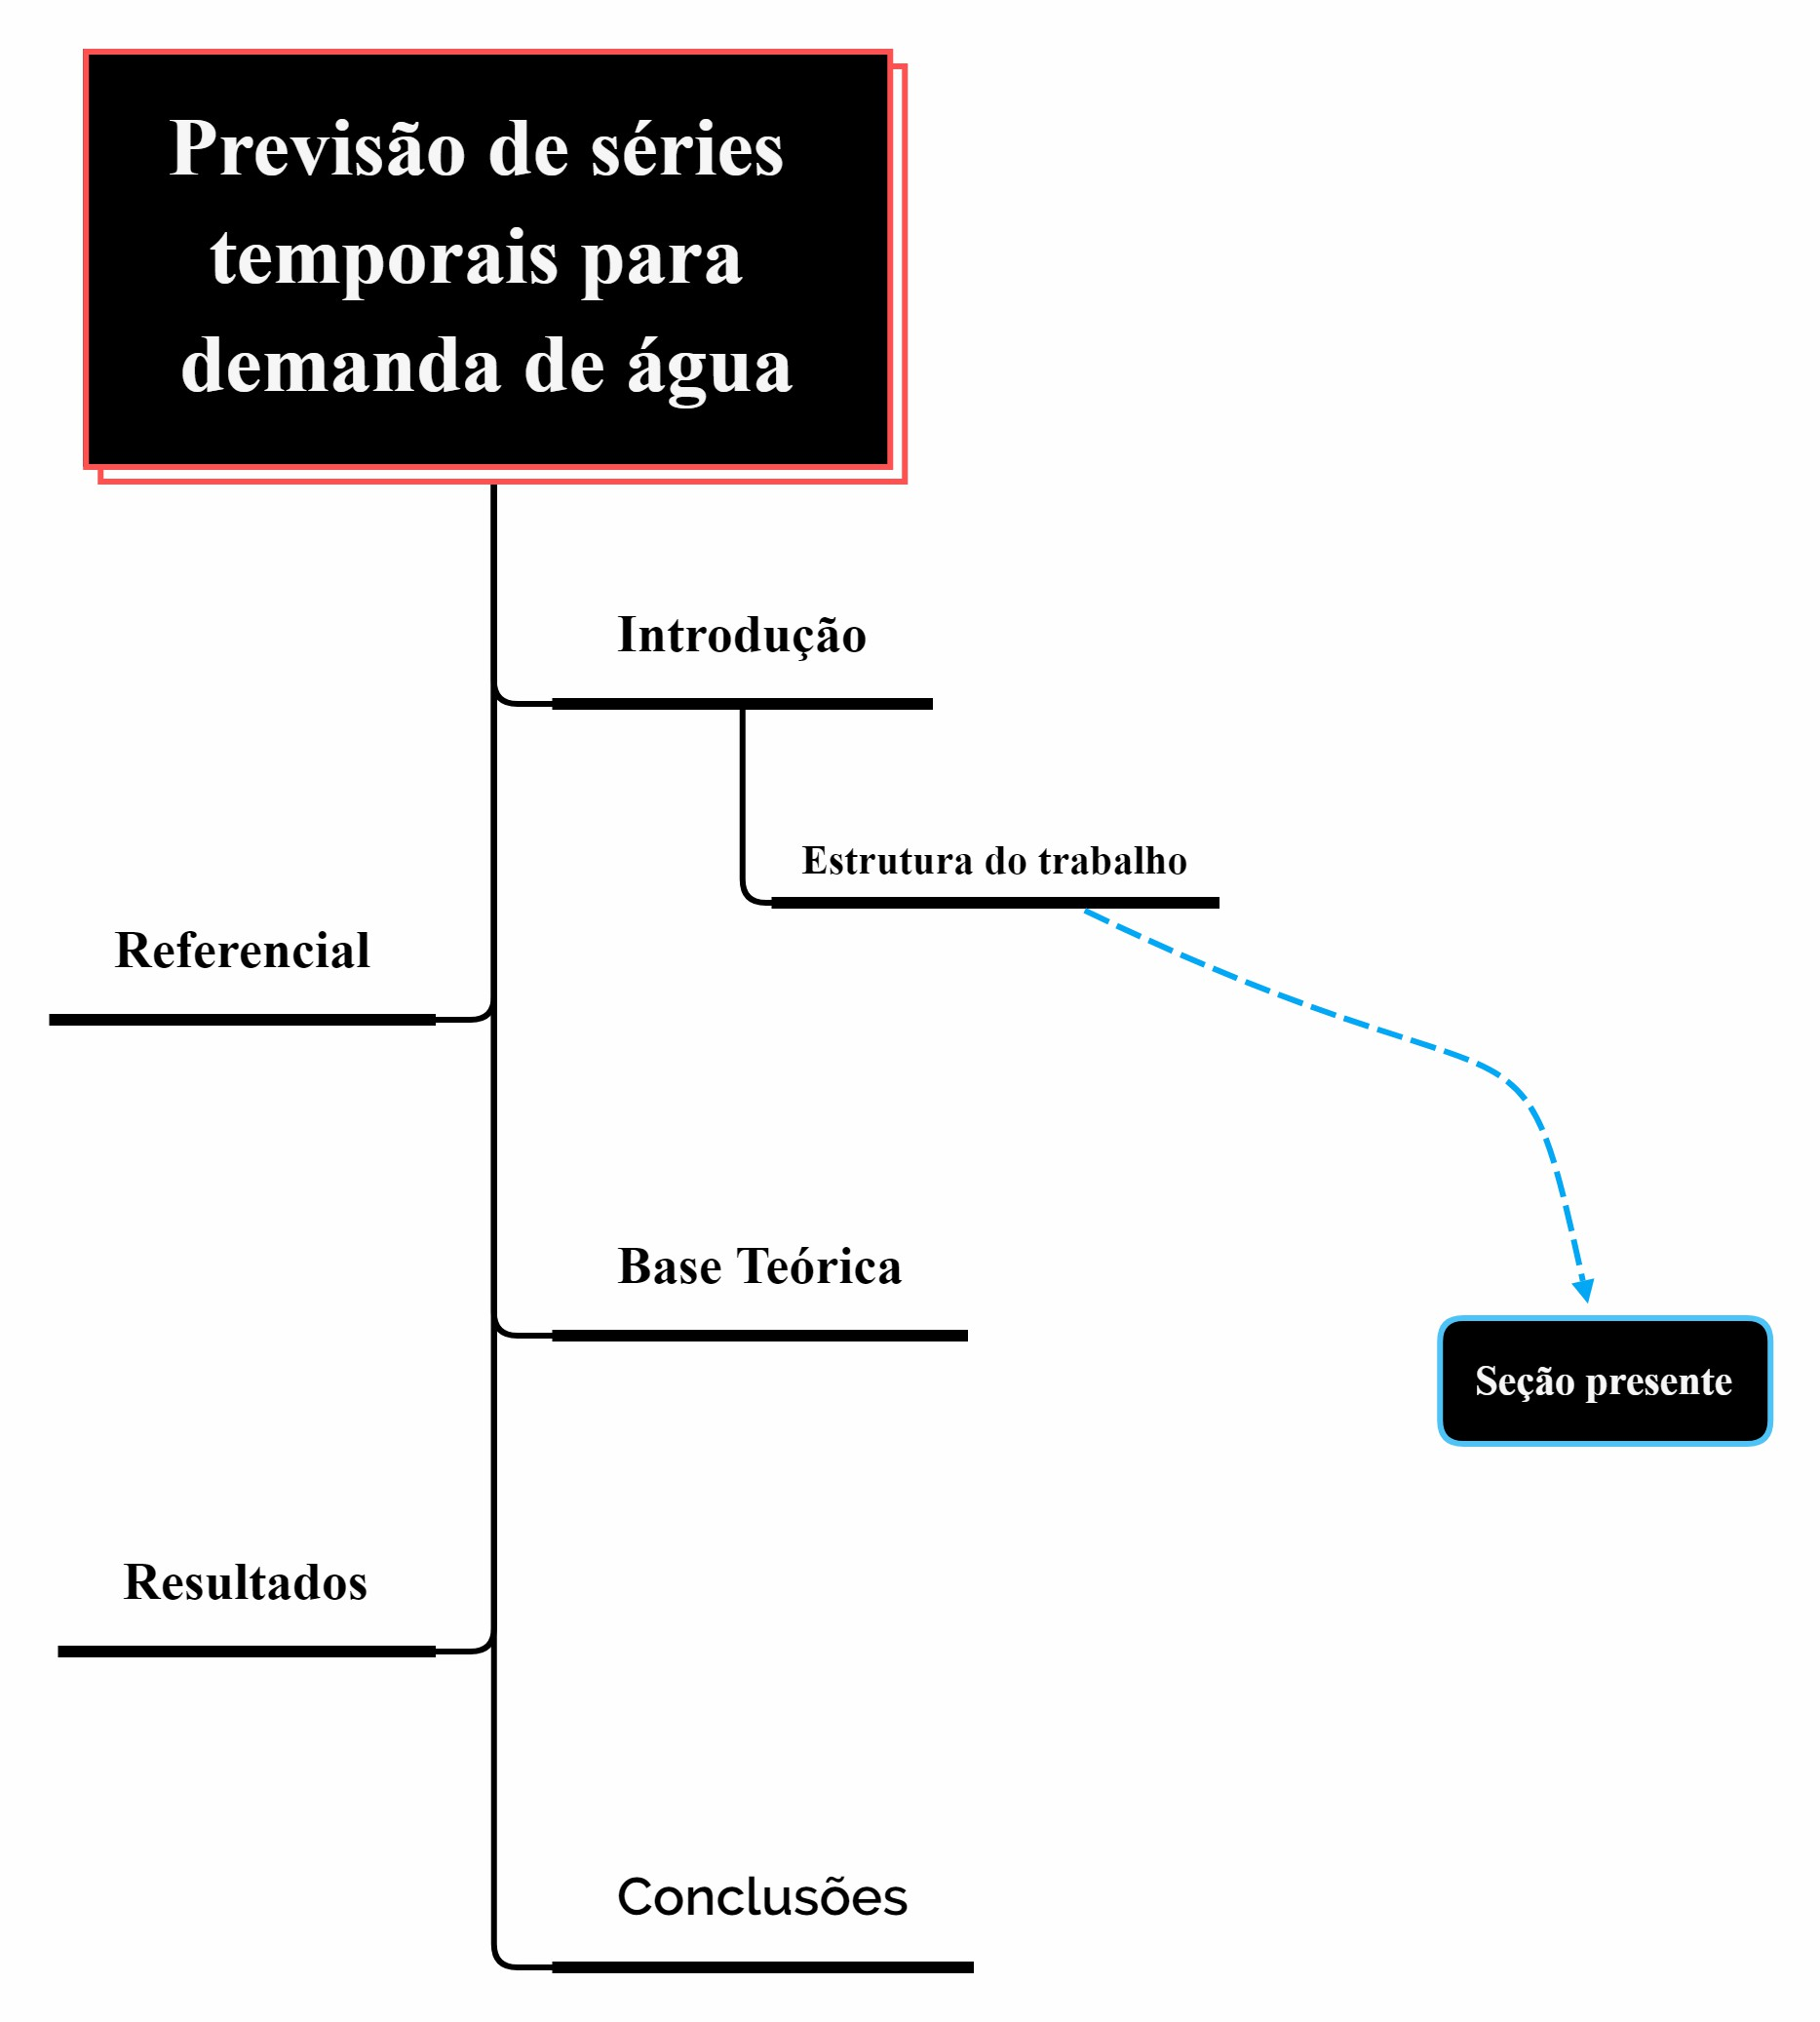
\includegraphics[width=0.7\linewidth]{Introducao/Figuras/Estrutura}
    	
    	Fonte: Elaboração própria 
    \end{figure}
O capítulo~\ref{sec:int} apresenta a introdução do trabalho, contendo a contextualização, a motivação, o objetivo geral, os objetivos específicos e a questão de pesquisa, a descrição do problema, a metodologia utilizada, a justificativa da pesquisa, as contribuições e a organização do trabalho.
O capítulo~\ref{sec:refteo} revisão teórica do trabalho, fazendo uma visão geral dos principais pesquisadores sobre as questões abordadas na pesquisa.
O capítulo~\ref{sec:base} apresenta os modelos que serão trabalhados nos dados coletados.
O capítulo~\ref{sec:result} apresenta os resultados da pesquisa, assim como uma análise dos resultados gerados.
O capítulo~\ref{sec:conclusoes}, finalmente, apresenta as considerações finais da pesquisa e algumas propostas para pesquisas futuras.



    
%% REFERENCIAL
\section{Revis\~ao da Literatura}\label{sec:refteo}


Este capítulo apresenta uma revisão sistemática  da literatura nos temas relacionados a previsão de séries temporais e aplicações em hidrologia e mais especificamente em abastecimento de água. A revisão bibliográfica realizada consiste em uma análise abrangente e crítica das principais fontes de literatura. Por meio dessa revisão, busca-se obter uma compreensão aprofundada do estado atual do conhecimento na área e identificar lacunas ou oportunidades de pesquisa. As informações extraídas da literatura são fundamentais para embasar a fundamentação teórica, a metodologia e a análise dos resultados da presente dissertação.

Esta revisão sistemática da literatura (RSL) aborda o tema das séries temporais, que é relevância em diversas áreas. A seleção das referências foi baseada em critérios específicos, levando em consideração a relevância dos autores, os países com maior número de publicações e as palavras-chave mais frequentes. Também foi incluído o tema saneamento básico, que é o foco dessa dissertação.

Embora nem todos os artigos revisados tenham uma relação evidente ou mesmo acentuada aprendizado de máquina (ML), eles contribuem como material de suporte a implementação de alguns modelos avaliados para previsão este trabalho e podem servir como base para outros pesquisadores.

A Figura \ref{fig:serie-temporal} apresenta um fluxograma de como a pesquisa foi realizada, destacando a importância dos autores como base para esta revisão da literatura. 

\begin{figure}[H]
	\centering
	\caption{Fluxograma do problema de pesquisa}
	\label{fig:serie-temporal}
	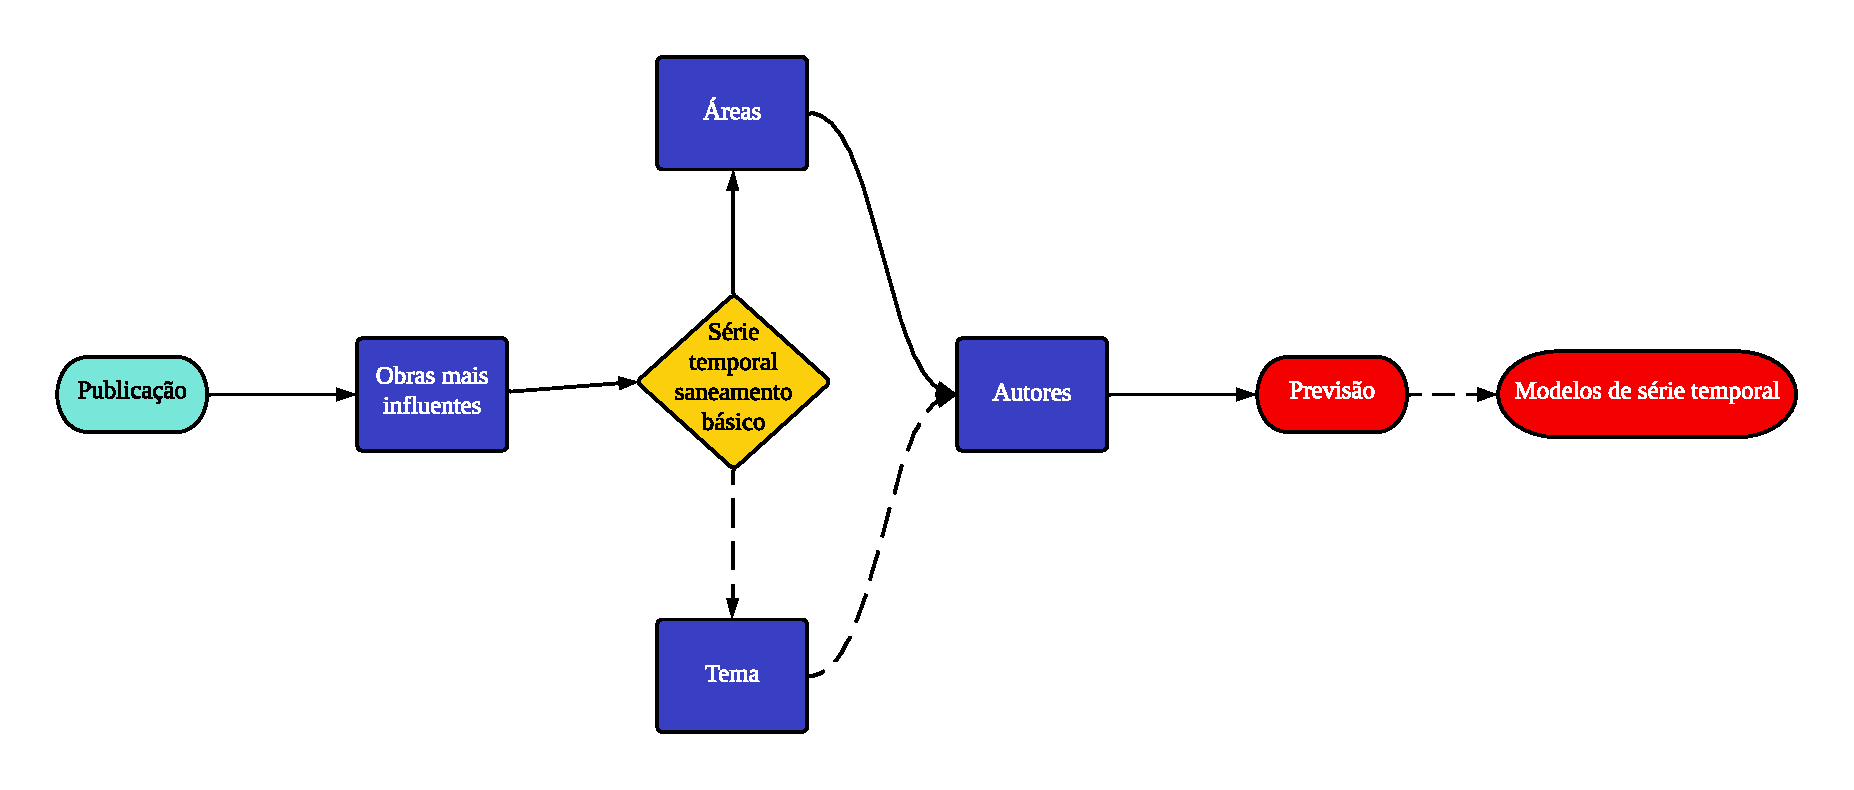
\includegraphics[width=\linewidth]{Revisao/Figuras/serie_temporal}
	
	
\end{figure}

A Figura \ref{fig:rsl} apresenta uma adaptação da metodologia proposta por \citeonline{MARTINS201671} para a realização desta RSL, foram realizadas buscas nos bancos de dados Scopus e WoS (\textit{Web of Science}), selecionando algumas bases relevantes para o tema da pesquisa.

\begin{figure}[H]
	\centering
	\caption{Etapas da revisão}
	\label{fig:rsl}
	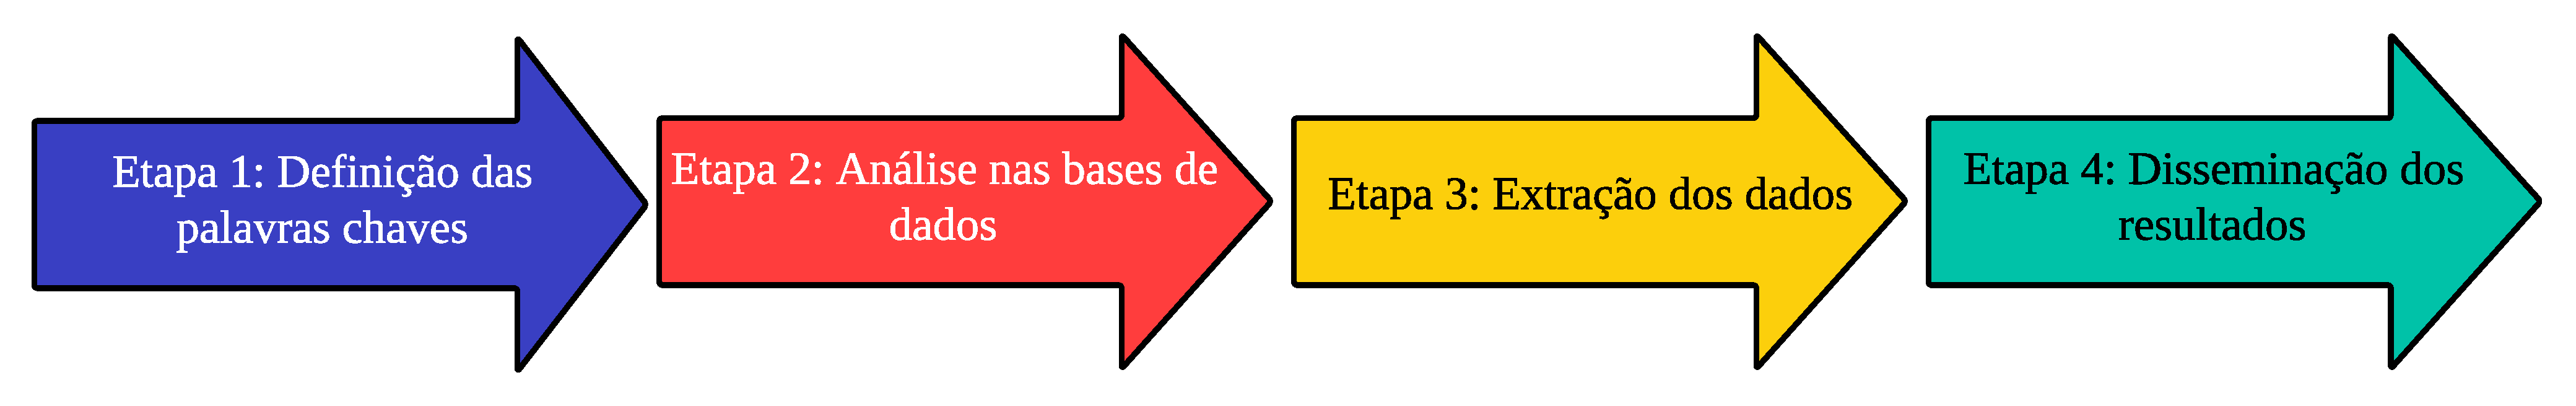
\includegraphics[width=\linewidth]{Revisao/Figuras/RSL}
	
	\fonte{Adaptado de \citeonline{MARTINS201671}}
\end{figure}

Para todas as bases de busca. Foram utilizadas palavras-chave que se adequam melhor à pesquisa, como ``\textit{time series forecasting}'', ``\textit{time series analysis}'', ``\textit{sanitation}'' e ``\textit{water supply}'' .


Na etapa seguinte, é realizada uma avaliação preliminar de cada artigo obtido, sem aplicar nenhum filtro anual nas buscas. Analisar todos os artigos dessa maneira resultaria em um número elevado, por exemplo, no banco de dados Scopus, existem 831 artigos, enquanto na WoS, são encontrados 98 artigos, totalizando 929 artigos sem a remoção de duplicatas. É importante ressaltar que esses artigos passaram apenas pelo filtro de idioma inglês e pela categoria de serem artigos, com o objetivo de aprimorar a busca e a tomada de decisões. Isso resulta em um número mais gerenciável de artigos para análise. Levando em consideração a diferença entre essa estimativa apresentada na Tabela \ref{tab:resumo} e a quantidade de artigos restantes após a remoção de duplicatas, tem-se menos de 929 artigos para análise. É válido lembrar que, ao remover as duplicatas, esse número pode diminuir ainda mais, chegando a 906 artigos, atingindo assim o objetivo proposto neste trabalho.

Na etapa final, é realizada uma análise aprofundada do conteúdo dos artigos selecionados, levando em consideração as áreas de especialização e correlação com séries temporais. Como esta revisão está inserida no contexto de um programa de mestrado em Engenharia de Produção e Sistemas, vale a pena analisar a correlação com áreas como Matemática. As áreas mais relevantes para a pesquisa são \textbf{``Informática'', ``Engenharia'' e ``Matemática''}, representando 50\% das publicações. Portanto, a pesquisa está alinhada com a utilização de conceitos matemáticos básicos para realizar uma estimativa do número de artigos.


São apresentados os resultados da pesquisa, utilizando um \textit{software} para melhor aproveitamento de cada banco de dados utilizado no trabalho. Inicialmente, é realizada uma análise no software VOSviewer.
A Figura \ref{fig:scopus-09-08} mostra os modelos que estão sendo usados com frequência, frequentemente utilizados como sinônimos ou em conjunto com ``\textit{time series}'' nos artigos. A análise da base de dados do Scopus é feita com uma ferramenta que exibe as palavras relacionadas em cada campo de busca, proporcionando uma visão abrangente das correlações com os modelos influentes.

\begin{figure}[H]
	\centering
	\caption{Modelos de series temporais mais populares na Scopus e WoS }
	\label{fig:scopus-09-08}
	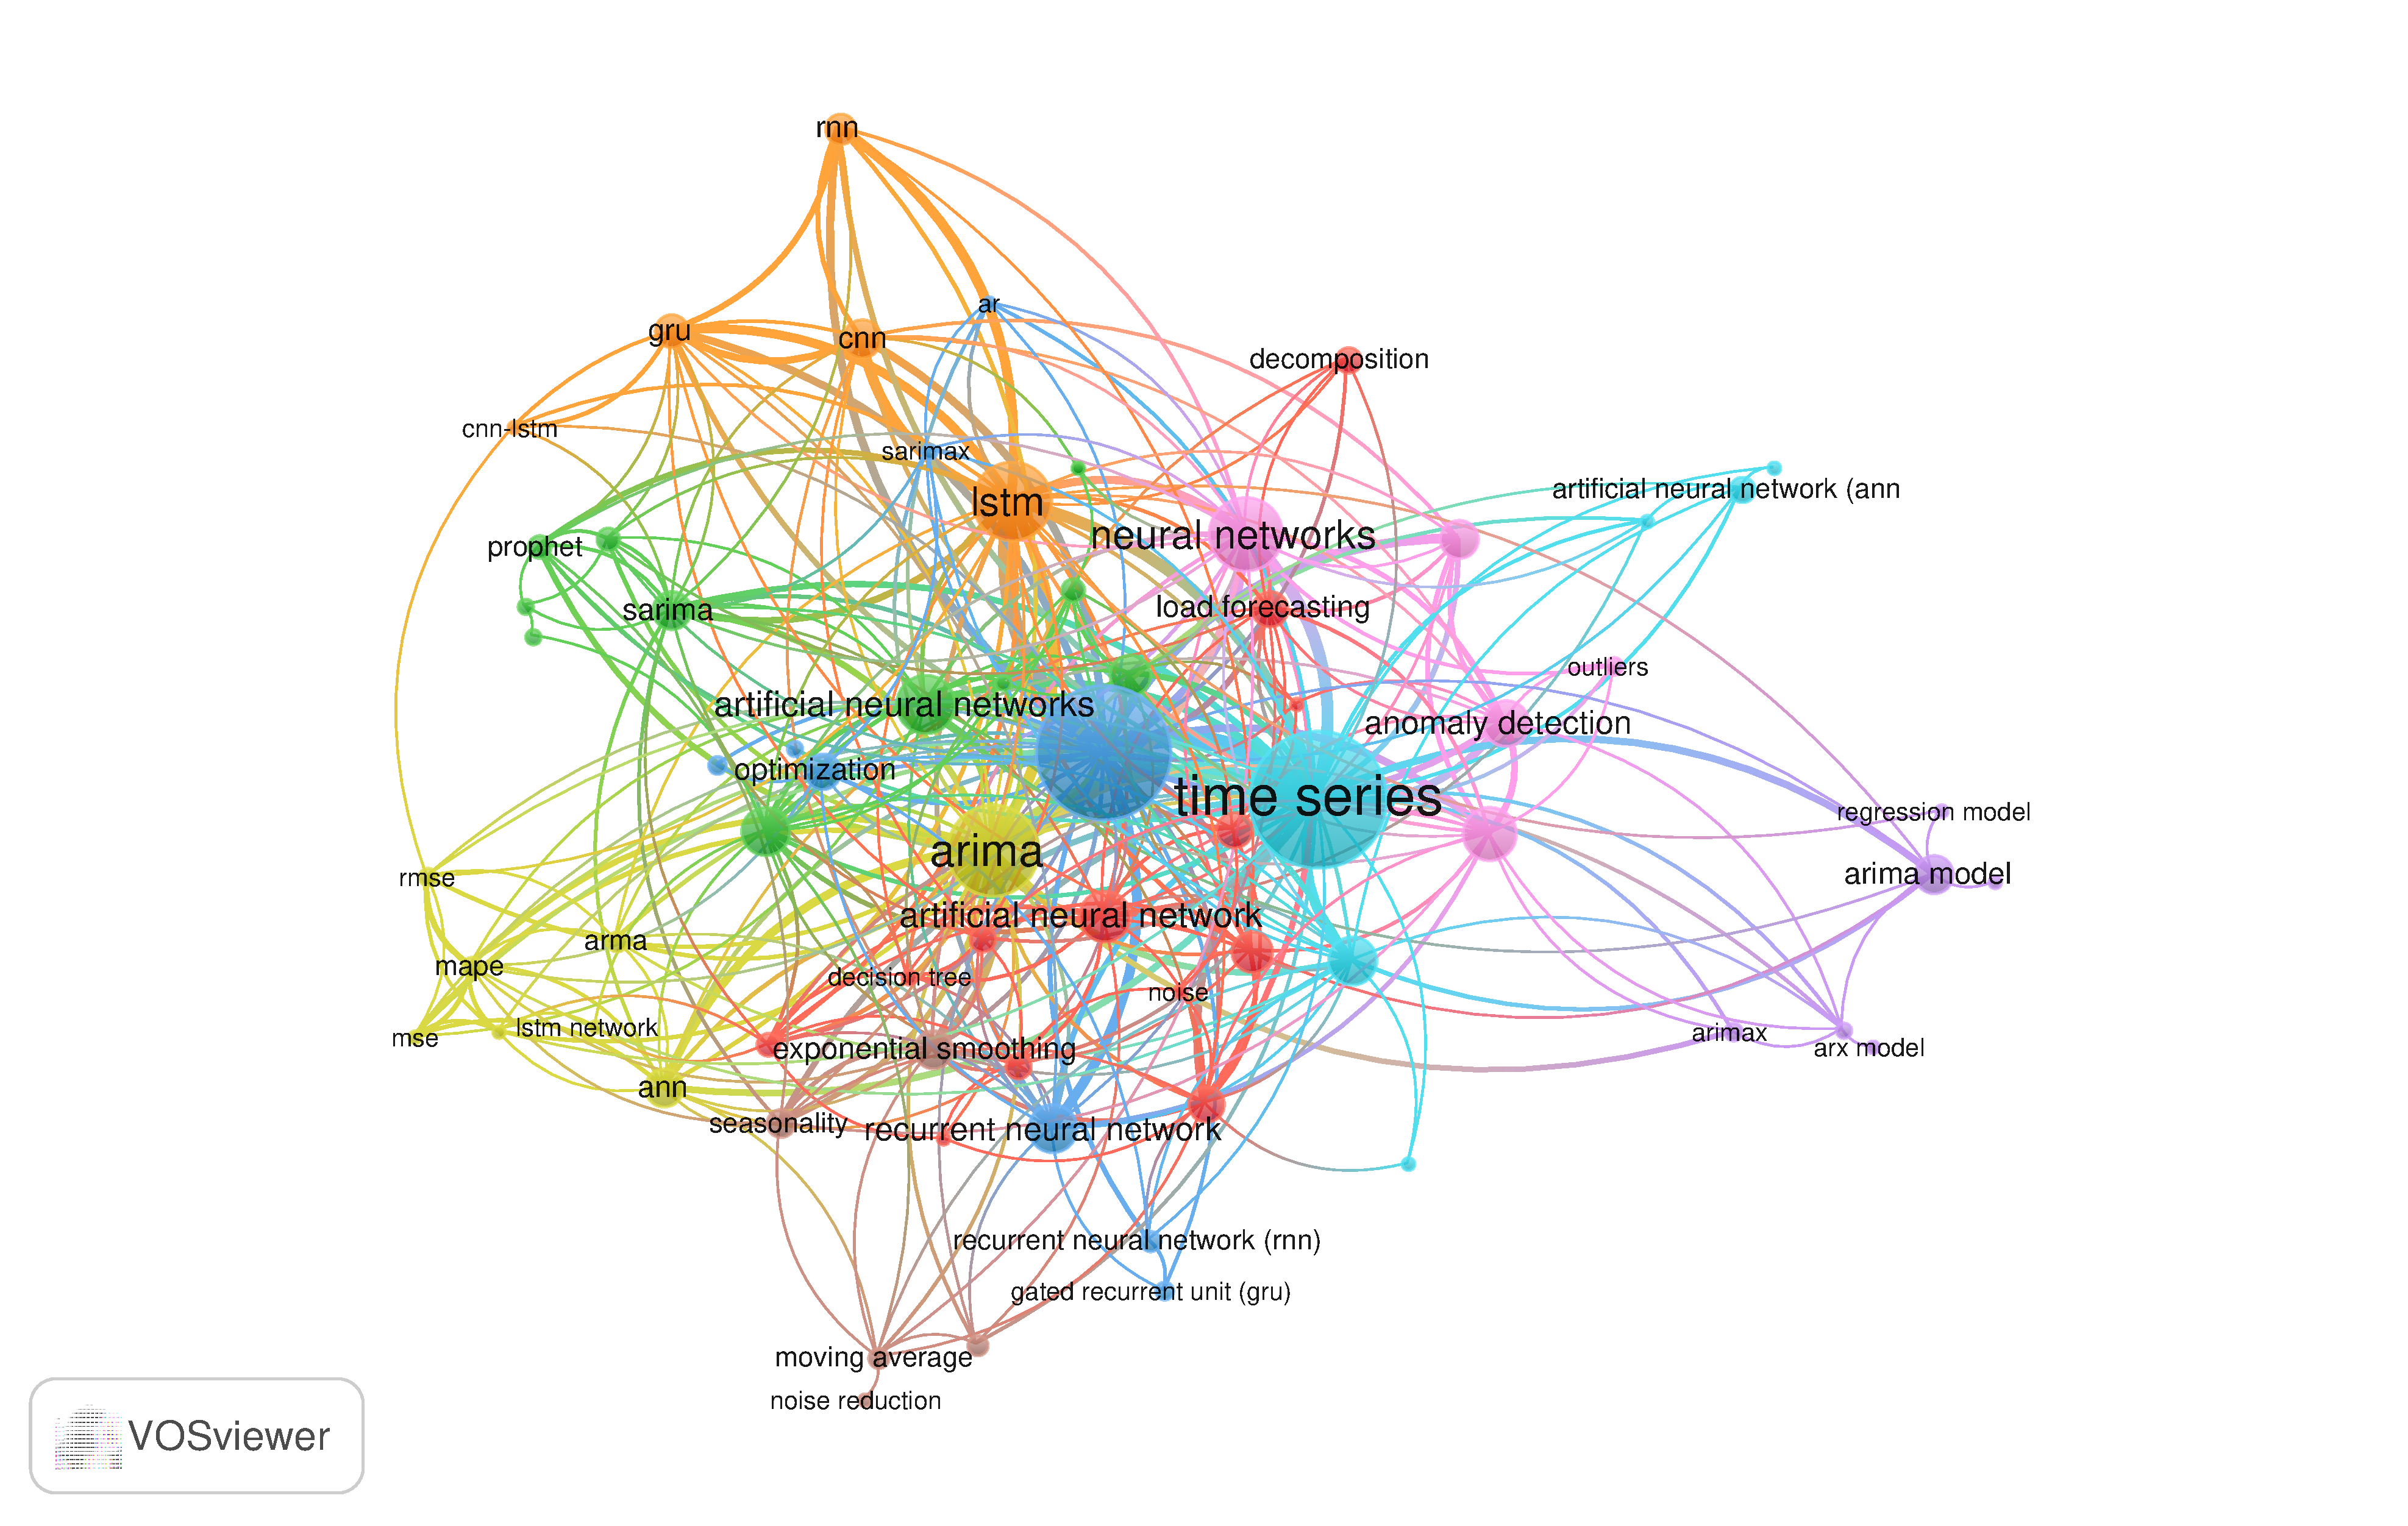
\includegraphics[width=\linewidth]{Revisao/Figuras/base-wos-scopus}
	
	
\end{figure}

Nesse primeiro momento, foram obtidos $2.555$ modelos, dos quais $83$ atingiram o limite estabelecido. É importante destacar que as palavras-chave base utilizadas são ``\textit{time series forecasting}'' ou ``\textit{time series analysis}'' e ``\textit{water supply}'' e ``\textit{sanitation}'' nas bases. Esses modelos obtidos podem estar repetidos, e é por isso que resultaram em um volume significativo de modelos.


A Tabela \ref{tb1} apresenta as palavras-chave utilizadas em cada base de dados, juntamente com o número de artigos encontrados inicialmente. No entanto, é importante ressaltar que esses dados ainda não foram processados para remover duplicatas. Após a utilização do software ScientoPy \cite{scientopy} para eliminar artigos repetidos, foram selecionados $308$ artigos únicos. Esses artigos representam a quantidade lida nesta RSL e são considerados relevantes para esta pesquisa.


\begin{table}[H]
	\centering
	\caption{Cruzamento de palavras-chave por meio da aplicação de filtros de área}\label{tb1}
	\begin{tabular}{@{}cp{2cm}cp{2cm}cp{1.5cm}cp{2cm}c@{}}
			\toprule
			Bases                   & \multicolumn{7}{c}{Palavras chaves}                                                          & Resultados \\ \midrule
			\multirow{2}{*}{Scopus} & time series forecasting & AND & time series analysis &     &              &     &            & 798        \\
			& time series forecasting & OR  & time series analysis & AND & water supply & AND & sanitation & 33         \\
			\multirow{2}{*}{WoS}    & time series forecasting & OR  & time series analysis &     &              &     &            & 79         \\
			& time series forecasting & OR  & time series analysis & AND & water supply & AND & sanitation & 19         \\ \hline
			\multicolumn{8}{c}{Total}                                                                                              & 929        \\ \bottomrule
		\end{tabular}
	
	
\end{table}



Na Tabela \ref{tab:resumo}, os dados coletados na RSL realizada no software ScientoPy \citeonline{scientopy} são apresentados. Nessa tabela, é exibida a quantidade de artigos coletados nas bases Scopus e WoS. Apesar de um volume considerável, nem todos os artigos foram lidos integralmente, uma vez que muitos deles não se relacionavam diretamente com o objeto de pesquisa. Consequentemente, ao longo da condução da RSL, esses artigos foram excluídos.

\begin{table}[H]
	\centering
	\caption{Resumo dos dados}
	\label{tab:resumo}
	\begin{tabular}{lc}
		\hline
		Dados Carregados & 929 \\
		Artigos Omitidos & 0 \\
		Total de Artigos & 929 \\
		Artigos da WoS & 98 \\
		Artigos do Scopus & 831 \\
		\hline
		\multicolumn{2}{c}{Remoção de Duplicados} \\
		\hline
		Porcentagem de Duplicados Encontrados & 87\% \\
		Artigos Duplicados Encontrados & 23 \\
		Contagem de Artigos Original & 929 \\
		Contagem de Artigos Atual & 906 \\
		Porcentagem de Duplicados Removidos da WoS & 19,4\% \\
		Porcentagem de Duplicados Removidos do Scopus & 0,5\% \\
		Artigos Duplicados com Diferentes Citações & 3 \\
		Porcentagem de Artigos Duplicados com Diferentes Citações & 13\% \\
		\hline
	\end{tabular}
	
	 
\end{table}


A Tabela \ref{tb2} apresenta os periódicos que mais publicaram artigos sobre o tema em questão. Todas os periódicos listadas, incluindo aquelas com um alto fator de impacto, como a categoria \textbf{Q1}, apresentam uma correlação significativa com as áreas de \textbf{informática, engenharia e matemática}.

\begin{table}[H]
	\centering
	\caption{Fator de impacto}\label{tb2}
	\begin{tabular}{@{}cp{3cm}p{3cm}c@{}}
		\toprule
		Periódicos      & Quantidade de plubicações & Qualidade do periódico & \textit{h-index} \\\midrule
		Neurocomputing         & 27                         & Q1                     & 143     \\
		IEEE Access            & 18                         & Q1                     & 127     \\
		Applied Soft Computing & 12                         & Q1                     & 143     \\
		Energies               & 11                         & Q2                     & 93      \\
		Energy                 & 11                         & Q1                     & 343     \\ \bottomrule
	\end{tabular}
	
	
	
\end{table}

Essa observação ressalta a importância dessas áreas de especialização na pesquisa sobre séries temporais. Esses periódicos desempenham um papel fundamental na disseminação do conhecimento e no avanço do campo, garantindo a qualidade e o impacto dos artigos publicados. Portanto, é relevante direcionar a atenção para esses periódicos, uma vez que são reconhecidas como fontes confiáveis e respeitadas dentro da comunidade científica.


O ScientoPy encontra os principais tópicos de tendência com base na maior taxa de crescimento médio (AGR do inglês \textit{average growth rate}). A AGR é a diferença média entre o número de documentos publicados em um ano e o número de documentos publicados no ano anterior \cite{scientopy}. Indica como o número de documentos publicados para um tópico cresceu (número positivo) ou diminuiu (número negativo) em média dentro de um período de tempo. Este AGR é calculado utilizando a equação \eqref{arg}:


\begin{eqnarray}
	\mathrm{AGR}&=&\dfrac{\sum_{i=Y_{\mathrm{s}}}^{Y_{\mathrm{e}}} P_i-P_{i-1}}{\left(Y_{\mathrm{e}}-Y_{\mathrm{s}}\right)+1} \label{arg}
\end{eqnarray}

\noindent onde AGR $=$ taxa média de crescimento; $Y_e =$ ano final; $Y_s =$ ano inicial; $P_i =$ número de publicações no ano $i$.
Para o ano final $Y_e$, o ScientoPy utiliza o ano final global por defeito configurado nas opções globais ou/em parâmetros do comando ScientoPy. O ano de início $Y_s$ é calculado a partir do ano final $Y_e$ , conforme indicado na equação \eqref{arg2}

\begin{eqnarray}
	Y_{\mathrm{s}}&=&Y_{\mathrm{e}}-(\text { WindowWidth }+1)\label{arg2}
\end{eqnarray}

A largura da janela (do inglês \textit{Window Width}) predefinido é de 2 anos. Assim, se o ano final for 2018, o AGR é a taxa de crescimento média entre 2017 e 2018 \cite{scientopy}.

A média de documentos por ano (ADY do inglês \textit{average documents per year}) é um indicador absoluto que representa o número médio de documentos publicados num período de tempo para um tópico específico. O ADY é calculado utilizando a equação \eqref{ady}:

\begin{eqnarray}
	\mathrm{ADY}&=&\dfrac{\sum_{i={Y_{\mathrm{s}}}(t)}^{Y_{\mathrm{e}}(t)} P_i}{\left(Y_{\mathrm{e}}(t)-Y_{\mathrm{s}}(t)\right)+1}\label{ady}
\end{eqnarray}

\noindent onde $ADY$ é a média de documentos por ano; $Y_e(t)$ é o ano final; $Y_s(t)$ é o ano inicial, calculado como descrito na equação \eqref{ady}; $Pi$ é o número de publicações no ano $i$.

A percentagem de documentos nos últimos anos (PDLY do inglês \textit{Percentage of documents in last years}) é um indicador relativo que representa a percentagem do ADY em relação ao número total de documentos para um tópico específico. Desta forma, o PDLY é calculado utilizando a equação \eqref{pdly}:

\begin{eqnarray}
	\mathrm{PDLY}&=&\dfrac{\sum_{i={Y_{\mathrm{s}}(t)}}^{Y_{\mathrm{e}}(t)} P_i}{\left(Y_{\mathrm{e}(t)}-Y_{\mathrm{s}(t)}+1\right) \cdot \mathrm{TND}} \cdot 100 \%\label{pdly}
\end{eqnarray}

\noindent onde $PDLY$ é a percentagem de documentos nos últimos anos; $Y_e(t)$ é o ano final; $Y_s$ é o ano inicial, calculado como descrito na equação \eqref{pdly}; $P_i$ é número de publicações no ano i; $TND$ é o número total de documentos.

Tabela \ref{tb:autor} para visualizar de forma mais clara os autores publicou sobre o tema em análise. Essa abordagem visa evitar a inclusão de todos os autores e destacar aquele que teve uma contribuição significativa no campo. Dessa forma, é possível identificar o principal autor que se destaca nesse tópico específico, fornecendo uma visão geral da distribuição da produção científica entre os pesquisadores.

Na Tabela \ref{tb:autor} apresenta a taxa de crescimento médio (AGR), documentos médios por ano (ADY) e percentagem de documentos nos últimos anos (PDLY) período: 2021 - 2023.

\begin{table}[H]
	\centering
	\caption{Os autores que mais publicam em relação ao tema de pesquisa}\label{tb:autor}
	\begin{tabular}{ccccccc}
		\hline
		Pos & Author       & Total & AGR  & ADY  & PDLY & \textit{h-index} \\
		\hline
		1 & \citeonline{2-s2.0-84973369468} & 11 & -0.5 & 2.0 & 36.4 & 8 \\
		2 & \citeonline{2-s2.0-85123707840} & 11 & 0.0 & 3.0 & 54.5 & 5 \\
		3 & \citeonline{2-s2.0-85018469706} & 10 & 1.0 & 2.5 & 50.0 & 5 \\
		4 & \citeonline{2-s2.0-85048003524} & 9 & -1.5 & 2.0 & 44.4 & 4 \\
		5 & \citeonline{2-s2.0-84964575877} & 7 & 1.5 & 2.0 & 57.1 & 3 \\
		6 & \citeonline{2-s2.0-85063200888} & 7 & 1.0 & 2.0 & 57.1 & 3 \\
		7 & \citeonline{2-s2.0-85148656225} & 7 & 1.0 & 3.0 & 85.7 & 2 \\
		8 & \citeonline{2-s2.0-85041536076} & 7 & 1.5 & 3.0 & 85.7 & 3 \\
		9 & \citeonline{2-s2.0-85130875471} & 6 & 0.0 & 1.5 & 50.0 & 4 \\
		10 & \citeonline{2-s2.0-85061810603}& 6 & 0.0 & 1.5 & 50.0 & 5 \\
		\hline
	\end{tabular}
	
	
\end{table}


A Tabela \ref{tb:pais}, que apresenta os países com maior número de publicações sobre o tema de saneamento básico, ordenados de forma decrescente. Os principais países que se destacam nessa análise são os seguintes: China, com $179$ publicações, Estados Unidos da América com $74$ publicações, Índia com $61$ publicações, Brasil com $49$ publicações, Espanha com $40$ publicações, Reino Unido com $40$ publicações, Austrália com $31$ publicações, Itália com $26$ publicações, Canadá com $25$, Irã com $20$ publicações.

\begin{table}[H]
	\centering
	\caption{Países com maior número de publicações}\label{tb:pais}
	\begin{tabular}{ccccccc}
		\toprule
		Pos & País & Total & AGR & ADY & PDLY & \textit{h-index} \\
		\midrule
		1 & China & 179 & 18.5 & 48.0 & 53.6 & 31 \\
		2 & Estados Unidos da América & 74 & 3.0 & 16.0 & 43.2 & 21 \\
		3 & Índia & 61 & 0.0 & 12.0 & 39.3 & 18 \\
		4 & Brasil & 49 & 3.5 & 12.5 & 51.0 & 17 \\
		5 & Espanha & 40 & 1.5 & 8.5 & 42.5 & 12 \\
		6 & Reino Unido & 40 & 3.0 & 10.0 & 50.0 & 15 \\
		7 & Austrália & 31 & 3.5 & 7.5 & 48.4 & 14 \\
		8 & Itália & 26 & 2.0 & 7.0 & 53.8 & 10 \\
		9 & Canadá & 25 & 1.0 & 5.5 & 44.0 & 11 \\
		10 & Irã & 20 & -1.0 & 3.5 & 35.0 & 11 \\
		\bottomrule
	\end{tabular}
	
	
\end{table}



Foi realizada uma investigação dos artigos na RSL. Esses artigos retratam alguns dos métodos utilizados em 
\citeonline{Taieb2016, Ursu2016, Wang2016, Graff2017, Tyralis2017, Boroojeni2017, Coelho2017, Chou2018, Bergmeir2018, Rossi2018, Ahmad2018, Chou2018a, Chen2018, Sadaei2019, Yang2019a, Buyuksahin2019, CarvalhoJr.2019, Liu2019, Shih2019a, Moon2019, Yang2019a, Xu2019, Golyandina2020, Martinovic2020a, Salgotra2020, Vlachas2020, Kulshreshtha2020, Samanta2020, Shen2020, Sezer2020, Du2020, Li2020,  Kumar2021, Lara-Benitez2021, Tan2021, Liu2021}.

Esses artigos abordam diferentes métodos usados pelos autores para previsão de séries temporais e análise não-linear dessas previsões. Eles representam contribuições significativas para o avanço do conhecimento e aplicação prática das séries temporais, sobre abordagens eficazes nesse campo. Ao incluir esses estudos influentes na análise, obtém-se uma visão abrangente dos métodos e técnicas  relevantes na previsão de séries temporais.

No estudo conduzido por \citeonline{Xu2019}, um modelo híbrido foi proposto, combinando o modelo linear AR e LR com o modelo não-linear ARIMA e o modelo DBN (do inglês \textit{Dynamic Bayesian Network}). Essa abordagem permitiu capturar tanto os comportamentos lineares quanto os não-lineares de uma série temporal. Por outro lado, \citeonline{Li2020} comparou o desempenho de previsão da abordagem MAELS (Modelo Alternativo de Estação Livre Série Temporal) com outros modelos de aprendizado de máquina de última geração, como ANN, CNN, RNN, LSTM, GRU, Transformer, Prophet, ARIMA e SVM-VAR (do inglês \textit{Support Vector Machine Variable Regression}). As abordagens ANN, CNN, RNN, GRU, Transformer e LSTM são capazes de lidar com dados multivariados de entrada e saída, enquanto o ARIMA utiliza informações passadas para prever o futuro com base em características como autocorrelação e médias móveis. Na Tabela \ref{tb:mode} é mostrado quantos artigos são relacionados em cada modelo que é utilizado neste trabalho e um artigo de cada modelo.



\noindent\textbf{Estudo de Caso 1: Adequação da Pressão e Vazão em uma Rede de Distribuição de Água}

\eqref{q1} Adequação da pressão atual para atender à demanda diária: Neste estudo de caso, o modelo SARIMAX foi utilizado para avaliar a adequação da pressão atual em uma rede de distribuição de água, considerando a demanda diária \cite{2-s2.0-85099424908}. O objetivo foi prever a pressão na rede com base em dados históricos, permitindo que fosse realizada uma análise da capacidade do sistema em atender às necessidades dos consumidores.

\eqref{q2} Volume mínimo de água no reservatório para evitar o acionamento das bombas: Para determinar o volume mínimo de água necessário no reservatório para evitar o acionamento das bombas durante o horário de pico, foi empregado um modelo DTR  \cite{2-s2.0-85054695177}. Este modelo ajudou a identificar regras e padrões que guiam a tomada de decisão sobre o nível de armazenamento ideal.

\eqref{q3} Vazão ótima para atender à demanda diária: O estudo também buscou encontrar a vazão ótima para atender à demanda diária. Para isso, utilizou-se o modelo XGBRegressor para otimizar a vazão na rede de distribuição, considerando as flutuações na demanda ao longo do dia \cite{2-s2.0-85130441623}.

\textbf{Estudo de Caso 2: Impacto do Acionamento das Bombas durante o Horário de Pico em uma Rede de Distribuição de Água}

\eqref{q5} Impacto do acionamento das bombas durante o horário de pico: Neste segundo estudo de caso, analisou-se o impacto do acionamento das bombas durante o horário de pico em uma rede de distribuição de água.

\ref{q5}\eqref{q5:a}, Nível ideal no reservatório e variação das vazões nos horários críticos: Utilizou-se o modelo ARIMA \cite{2-s2.0-85069459067} para prever o nível ideal no reservatório e analisar as variações das vazões nos horários críticos, levando em consideração as diferentes estações do ano.

\ref{q5}\eqref{q5:b}, Tendência, padrão e sazonalidade nos dados do Bairro Alto: Para identificar tendências, padrões e sazonalidades nos dados de três anos do Bairro Alto, empregou-se o modelo de decomposição STL, reconhecido por sua eficácia na modelagem de séries temporais com essas características.

\ref{q5}\eqref{q5:c}, Identificação dos horários de maior demanda: A identificação dos horários de maior demanda entre as 18h e as 21h foi realizada com o uso da RNN (P) \cite{2-s2.0-85067419084}.

\ref{q5}\eqref{q5:d}, Tendência, padrão e sazonalidade nos dados de abastecimento de água do Bairro Alto: Para identificar tendências, padrões e sazonalidades nos dados relacionados a demanda de água de três anos do Bairro Alto, empregou-se o modelo decomposição STL, reconhecido por sua eficácia na modelagem de séries temporais com essas características. O volume de armazenamento no reservatório para evitar o acionamento das bombas: Determinar a quantidade de água a ser armazenada previamente no reservatório para evitar o acionamento das bombas durante o horário de pico envolveu o modelo LGBMRegressor.

\ref{q5}\eqref{q5:e}, Tendência, Padrão e Sazonalidade nos Dados do Bairro Alto: Para identificar tendências, padrões e sazonalidades nos dados de três anos do Bairro Alto, empregou-se o modelo STL, reconhecido por sua eficácia na modelagem de séries temporais com essas características. Detecção de anomalias na rede com base no histórico): Para detectar anomalias na rede com base no histórico de vazão e pressão, utilizou-se novamente o modelo ARX \cite{2-s2.0-85051469381}.

Cada estudo de caso abordou questões específicas relacionadas ao sistema de abastecimento de água e utilizou modelos apropriados para cada tarefa. Isso permitiu uma análise detalhada das diferentes facetas do problema.

\begin{table}[H]
	\centering
	\caption{Modelos baseado na literatura e nos artigos}\label{tb:mode}
	\begin{tabular}{ccccccc}
		\toprule
		Pos & Palavras-chave & Total & AGR & ADY & PDLY & \textit{h-index} \\
		\midrule
		1 & ARIMA, \citeonline{2-s2.0-85069459067} & 84 & 1.7 & 16.7 & 59.5 & 27 \\
		2 & ANN, \citeonline{2-s2.0-85054695177} & 36 & 0.7 & 9.0 & 75.0 & 17 \\
		3 & LSTM, \citeonline{WOS:000529902300014} & 35 & 3.3 & 10.7 & 91.4 & 16 \\
		4 & RNN, \citeonline{2-s2.0-85067419084} & 20 & 0.0 & 4.3 & 65.0 & 11 \\
		5 & Árvores de Decisão, \citeonline{2-s2.0-85054695177} & 12 & 0.7 & 3.0 & 75.0 & 7 \\
		6 & Transformer, \citeonline{2-s2.0-85045193200} & 10 & 2.3 & 3.0 & 90.0 & 5 \\
		7 & Random Forest, \citeonline{2-s2.0-85135210428} & 9 & 1.7 & 2.7 & 88.9 & 5 \\
		8 & CNN, \citeonline{WOS:000841076700002} & 8 & 1.3 & 2.7 & 100.0 & 4 \\
		9 & ARMA, \citeonline{2-s2.0-85038637324} & 7 & 0.3 & 0.7 & 28.6 & 6 \\
		10 & GRU, \citeonline{2-s2.0-85135210428} & 5 & 0.0 & 1.3 & 80.0 & 4 \\
		11 & SARIMA, \citeonline{2-s2.0-85128561644} & 5 & 1.0 & 1.7 & 100.0 & 4 \\
		12 & ARX, \citeonline{2-s2.0-85051469381} & 3 & 0.0 & 0.7 & 66.7 & 2 \\
		13 & LR, \citeonline{2-s2.0-85125426780} & 3 & 0.0 & 0.7 & 66.7 & 3 \\
		14 & Prophet, \citeonline{2-s2.0-85092514286} & 3 & 0.3 & 1.0 & 100.0 & 3 \\
		15 & MAPE, \citeonline{2-s2.0-85097173237} & 2 & 0.0 & 0.7 & 100.0 & 1 \\
		16 & MSE, \citeonline{2-s2.0-85096470870} & 2 & 0.0 & 0.3 & 50.0 & 2 \\
		17 & SARIMAX,\citeonline{2-s2.0-85099424908} & 2 & 0.3 & 0.7 & 100.0 & 2 \\
		18 & MAE, \citeonline{2-s2.0-85082955699} & 1 & 0.0 & 0.3 & 100.0 & 1 \\
		19 & XGBoost, \citeonline{2-s2.0-85130441623} & 1 & 0.3 & 0.3 & 100.0 & 0 \\
		\bottomrule
	\end{tabular}
	
	
	
\end{table}


Dessa forma, por meio dessa revisão sistemática e análise de conteúdo.
Além desses modelos mencionados, também será utilizada a versão atualizada do ARIMA nesta dissertação. Os modelos SARIMA e SARIMAX também serão comparados para determinar qual deles é o mais adequado. Além disso, serão empregados os modelos Light GBM e XGBoost. Os modelos de aprendizado profundo, como a RNN, ainda são considerados os melhores modelos para séries temporais no tema de saneamento básico que está sendo abordado.

Quanto a modelos, tais como RNN, CNN, ANN, LSTM, Transformer, GRU, Light GBM, XGBoost, RFR, DTR e LR, não fossem encontrados na literatura relacionados a  saneamento básico. 
Embora existam várias ramificações do modelo ARIMA, o modelo desenvolvido pelo Facebook, conhecido como Prophet, sobressai como uma opção superior em comparação com os demais. O Prophet é um modelo mais recente que simplifica significativamente muitas das tarefas que são necessárias ao lidar com o ARIMA. Enquanto o Prophet foi criado em 2017, o modelo ARIMA tem relatos de ter sido desenvolvido na década de 1960. Essa diferença temporal destaca a evolução e a modernização do campo de modelagem de séries temporais ao longo das décadas \cite{ramos2010previsoes}.












\section{Base Te\'orica}\label{sec:base}

A base teórica é fundamental para se obter resultados satisfatórios, pois ela proporciona um sólido conhecimento sobre o tema em questão. Neste capítulo, são abordados diversos aspectos relevantes, incluindo métricas de erro e modelos regressivos de previsão. Essas métricas desempenham um papel crucial na avaliação e comparação dos modelos, permitindo uma análise precisa do desempenho de cada um. Além disso, os modelos regressivos de previsão são explorados, fornecendo insights valiosos sobre como essas técnicas podem ser aplicadas para realizar previsões com precisão. Compreender e dominar esses conceitos é essencial para se obter resultados confiáveis e embasar as próximas etapas do trabalho de pesquisa.



\subsection{Modelos de S\'eries Temporais Univariados}\label{subsec:arima}

A previsão de séries temporais é um desafio complexo, sem uma resposta fácil. Existem inúmeros modelos estatísticos que afirmam superar uns aos outros, mas nunca está claro qual modelo é o melhor.

Dito isto, os modelos baseados em ARMA são frequentemente uma boa opção para iniciar. Eles podem alcançar pontuações decentes na maioria dos problemas de séries temporais e são adequados como modelos de referência em tais problemas.

Quanto ao modelo ARIMA, ele é dividido em três componentes: AR (Auto-Regressão), I (Integração) e MA (Média Móvel). O componente AR leva em consideração os valores anteriores da série temporal, o componente I trata das diferenças entre os valores observados para tornar a série estacionária, e o componente MA considera os erros residuais do modelo. Esses componentes combinados ajudam a capturar os padrões e tendências presentes na série temporal.

\subsubsection{Componente Autorregressivo}

O componente autoregressivo do modelo ARIMA é representado por AR(p), em que o parâmetro p determina o número de séries temporais defasadas utilizadas.

A equação do modelo AR(p) é expressa da seguinte forma:

\begin{eqnarray}
	Y_t&=&c+\sum_{n=1}^{p} \alpha_n Y_{t-n} + \varepsilon_t\label{AR}
\end{eqnarray}

A partir dos dados, é possível obter uma previsão utilizando o modelo AR(7).

\begin{figure}[!htb]
	\centering
	\caption{Comparação dos modelos AR e ARX}
	\begin{subfigure}{1\textwidth}
		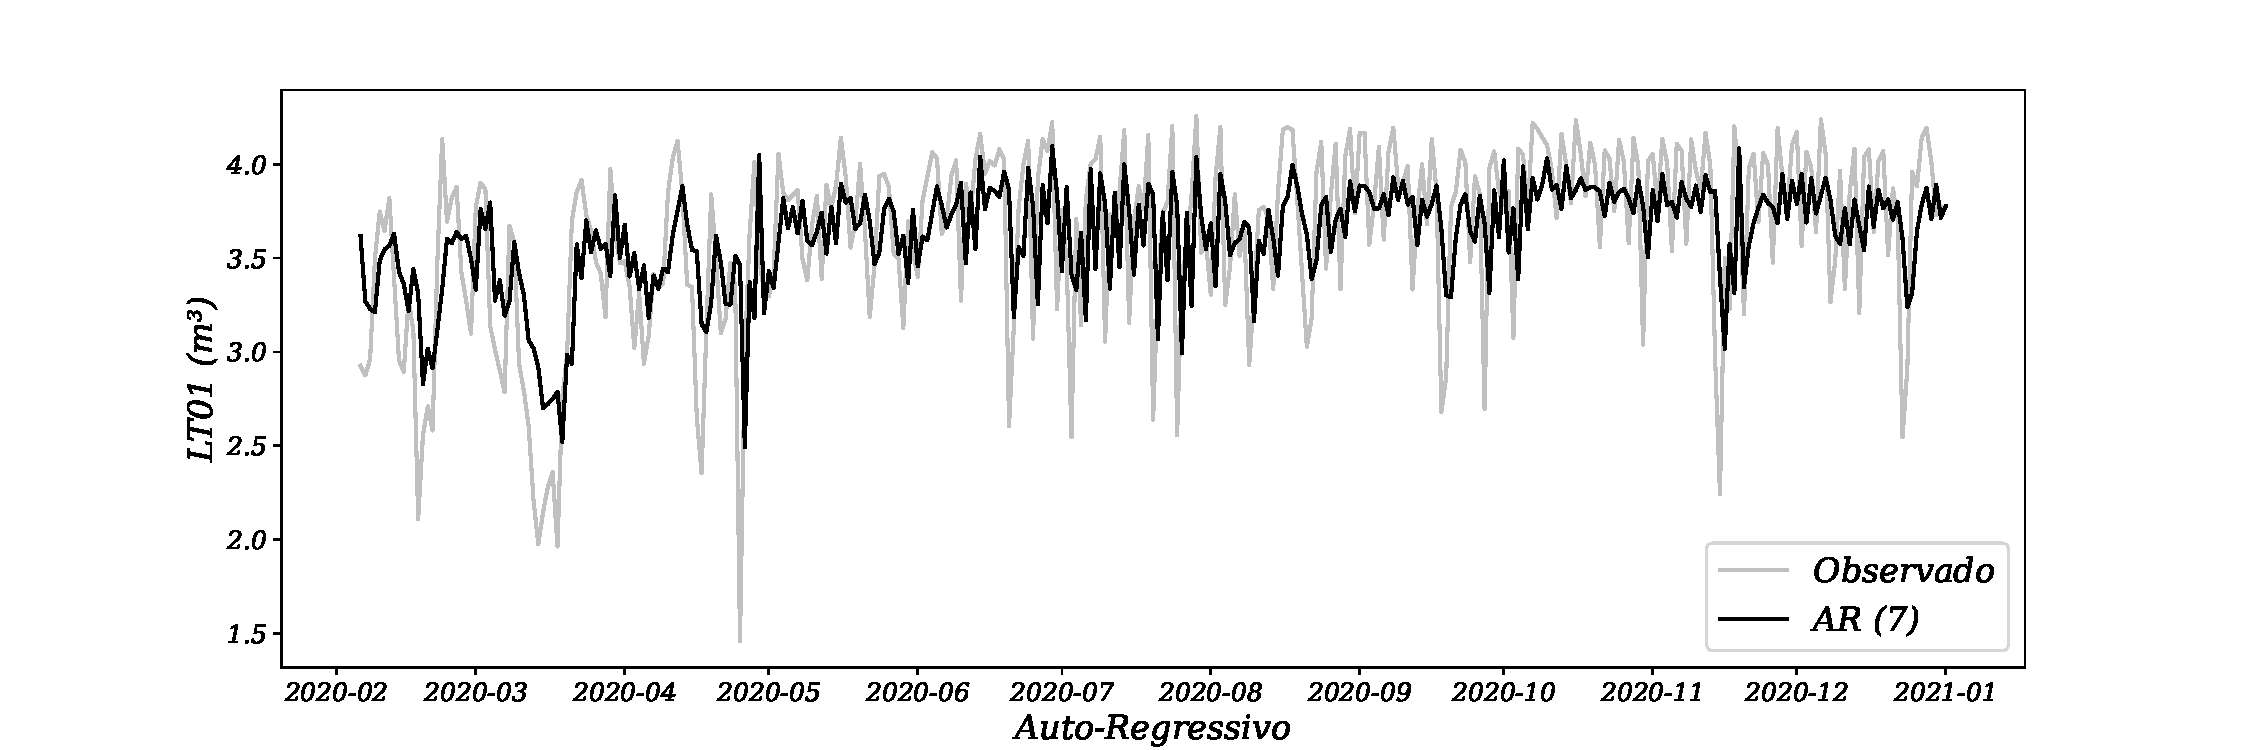
\includegraphics[width=\linewidth]{Modelos/Figuras/AR}
		\caption{Modelo AR(7)}
		\label{fig:1-ar}	
	\end{subfigure}
	
	\begin{subfigure}{1\textwidth}
		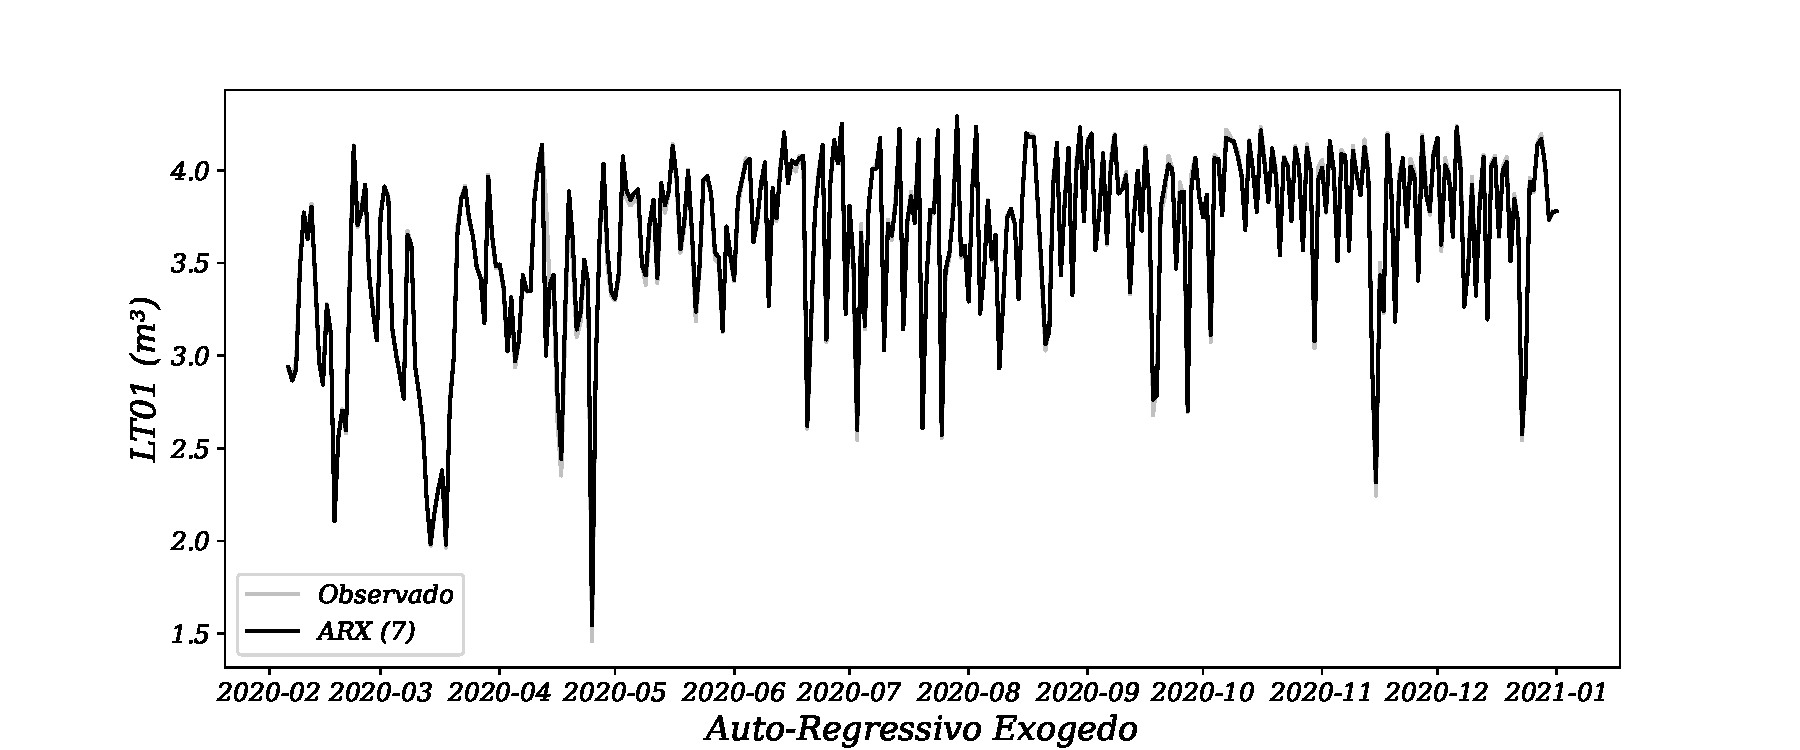
\includegraphics[width=\linewidth]{Modelos/Figuras/ARX}
		\caption{ARX (7)}
		\label{fig:1-arx}	
	\end{subfigure}
	
	\fonte{Elaboração própria a partir de dados da SANEPAR (2018 a 2020)}
\end{figure}



Na equação \eqref{AR}, o termo $\varepsilon_t$ representa o ruído branco. Essa equação pode ser entendida como uma regressão múltipla, em que os valores defasados de $y_t$ são utilizados como preditores. Esse modelo é conhecido como modelo autorregressivo de ordem $p$, ou AR(p).

A Figura \ref{fig:1-ar} tem como objetivo apresentar uma previsão de um passo à frente (um dia). Nos apêndices \ref{sec:ararxma24}, pode-se observar uma comparação entre os modelos AR, MA e ARX.

O modelo ARX é uma extensão do modelo AR, que incorpora variáveis exógenas nos dados para melhorar as previsões futuras. Esse modelo também é multivariado, como mostrado na subseção \ref{subsec:mult}, e foi incluído aqui para fins de comparação com o modelo AR simples, considerando a presença de variáveis exógenas.

Embora o modelo AR possa ser visualmente adequado para a previsão que está sendo feita, é importante destacar que, por ser um modelo autorregressivo, ele realiza previsões lineares e não captura padrões não lineares presentes nos dados. Para uma análise mais abrangente da série temporal, é necessário considerar exemplos de casos gerais.

\subsubsection{AR(0): Ru\'ido branco}

Se o parâmetro $p$ for definido como zero (AR($0$)), significa que não há termos autorregressivos no modelo. Nesse caso, a série temporal se comporta como um ruído branco. Cada ponto de dados é amostrado de uma distribuição com média zero e variância igual a sigma-quadrado. Isso resulta em uma sequência de números aleatórios que não exibem nenhum padrão ou correlação.

Essa propriedade do ruído branco pode ser útil em análises estatísticas, pois serve como uma hipótese nula. Ao comparar diferentes modelos ou testar a presença de padrões em uma série temporal, podemos usar o ruído branco como referência para avaliar se os resultados observados são estatisticamente significativos ou apenas resultado do acaso. Isso nos ajuda a evitar a detecção de padrões falsos positivos e garante a confiabilidade das análises realizadas.

\subsubsection{AR(1): Caminhadas aleat\'orias e Oscila\c c\~oes}

Com o parâmetro $p$ definido como $1$, o modelo AR leva em consideração o valor anterior da série temporal multiplicado por um coeficiente e, em seguida, adiciona ruído branco. Quando o coeficiente é igual a $0$, temos apenas ruído branco, resultando em uma série de tempo completamente aleatória, sem padrões previsíveis.

Quando o coeficiente é igual a $1$, temos uma caminhada aleatória, onde cada valor da série é obtido somando-se o valor anterior a um termo de ruído branco. Nesse caso, os valores da série apresentam uma tendência linear, aumentando ou diminuindo ao longo do tempo sem retornar à média.

Se o coeficiente estiver na faixa $0 < \alpha < 1$, temos o fenômeno de reversão média. Isso significa que os valores da série tendem a oscilar em torno de uma média central e a regressar em direção a ela após se afastarem. Esse padrão indica uma tendência de retorno à média ao longo do tempo.

Os diferentes comportamentos da série temporal, determinados pelo coeficiente no modelo AR, têm implicações importantes na análise e previsão de dados. A compreensão desses padrões é fundamental para escolher o modelo adequado e interpretar corretamente os resultados obtidos.

\subsubsection{AR(p): Termos de ordem superior}

Aumentar ainda mais o parâmetro $p$ no modelo AR significa considerar um número crescente de medições de tempo anteriores, cada uma multiplicada pelo seu próprio coeficiente. Isso permite levar em conta uma memória mais longa da série temporal e capturar padrões de dependência mais complexos ao longo do tempo.

No entanto, é importante ter em mente que aumentar excessivamente o valor de $p$ pode levar a problemas de \textit{overfitting}, onde o modelo se ajusta muito bem aos dados de treinamento, mas tem um desempenho ruim na previsão de novos dados. Portanto, é necessário encontrar um equilíbrio entre a complexidade do modelo e sua capacidade de generalização.

Além disso, é comum combinar o modelo AR com o modelo de média móvel (MA) para formar o modelo ARMA. O modelo MA considera os erros passados, ou seja, as diferenças entre os valores reais e as previsões anteriores, ajustadas por coeficientes. A combinação dos componentes AR e MA permite capturar tanto a dependência autorregressiva quanto a dependência na média móvel, proporcionando uma modelagem mais abrangente da série temporal.

Em suma, aumentar o parâmetro $p$ no modelo AR pode melhorar a capacidade do modelo de capturar padrões complexos da série temporal, mas é necessário ter cuidado para evitar \textit{overfitting}. A combinação com o modelo MA pode fornecer uma modelagem mais completa dos dados. A escolha adequada dos parâmetros depende da análise cuidadosa dos padrões presentes na série temporal e do equilíbrio entre a complexidade do modelo e sua capacidade de generalização.

\subsubsection{M\'edia M\'ovel}\label{subsubsec:ma}
No modelo de média móvel (MA), o componente não é uma média móvel simples, mas sim uma combinação de termos de erro de previsão defasados. O parâmetro $q$ no modelo MA representa o número de termos de erro de previsão que são levados em consideração na previsão.

De acordo com \citeonline{signal} este componente não é uma média de rolamento, mas sim os atrasos no ruído branco.

Em um modelo MA(1), por exemplo, a previsão é composta por um termo constante, o produto do termo de erro de previsão anterior por um multiplicador, e o termo de erro de previsão atual. Essa abordagem baseia-se em princípios estatísticos e de probabilidade, ajustando a previsão com base em termos anteriores de erro de previsão.

O modelo MA é uma alternativa ao modelo AR e é usado para capturar padrões de dependência na média móvel, ou seja, a influência de erros passados na previsão atual. Ao combinar o modelo AR e o modelo MA, como no modelo ARMA, é possível obter uma modelagem mais abrangente que considera tanto a dependência autorregressiva quanto a dependência na média móvel.

Portanto, o modelo MA leva em conta os termos de erro de previsão defasados para ajustar a previsão atual, permitindo considerar a probabilidade e estatística na modelagem da série temporal.


\begin{eqnarray}
	y_t=c+\varepsilon_t+\theta_1 \varepsilon_{t-1}+\theta_2 \varepsilon_{t-2}+\cdots+\theta_q \varepsilon_{t-q}\label{eq:ma}
\end{eqnarray}

Na equação \eqref{eq:ma}, em que $\varepsilon_t$ representa o ruído branco, esse modelo é conhecido como um modelo de média móvel $MA(q)$, em que $q$ é a ordem da média móvel. É importante ressaltar que não observamos diretamente os valores de $\varepsilon_t$, portanto, essa modelagem não se trata de uma regressão no sentido convencional.

Diferentemente de uma regressão comum em que temos variáveis explicativas observadas, no modelo $MA(q)$, estamos usando os termos de ruído branco defasados para estimar e prever os valores da série temporal. O objetivo é capturar a dependência dos termos de erro passados na previsão atual.

Esse modelo é útil para modelar séries temporais em que a média móvel tem um impacto significativo nas observações. Ao ajustar a série temporal com base nos termos de ruído branco defasados, podemos obter uma estimativa mais precisa dos valores futuros.

Embora o modelo $MA(q)$ seja diferente de uma regressão tradicional, ele é uma ferramenta estatística poderosa para modelar e prever séries temporais, levando em consideração a dependência entre os termos de erro passados.

\begin{figure}[!htb]
	\centering
	\caption{Modelo MA(7) }
	\label{fig:1-ma}
	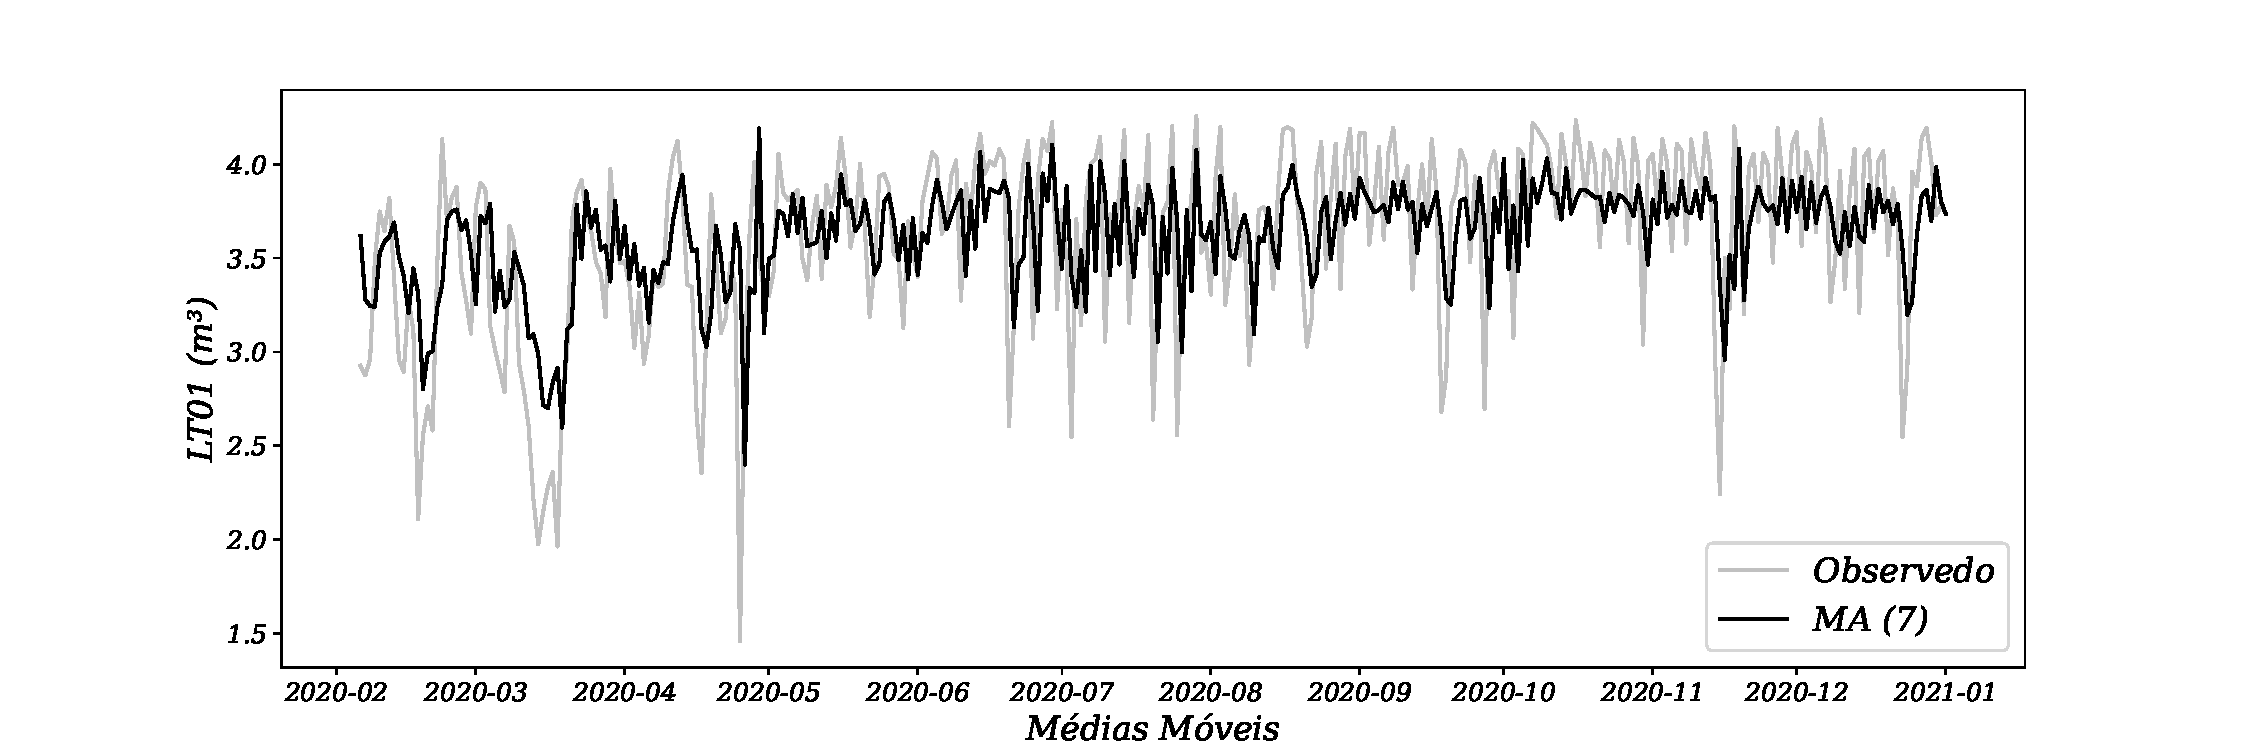
\includegraphics[width=1\linewidth]{Modelos/Figuras/MA}
	
	\fonte{Elaboração própria a partir de dados da SANEPAR (2018 a 2020)}
\end{figure}

O modelo MA, quando comparado com o modelo AR de mesma ordem, facilita a previsão. Conforme ilustrado na Figura \ref{fig:1-ma}, a previsão gráfica se assemelha ao modelo apresentado na Figura \ref{fig:1-ar}, embora não seja comparável ao modelo exibido na Figura \ref{fig:1-arx}. É importante notar que esse modelo aparenta prever com precisão o período de tempo que foi considerado.

\subsubsection{Modelos ARMA e ARIMA}\label{subsubsec:arma}
A arquitetura ARMA é uma combinação dos modelos AR  e MA, onde o modelo AR é adicionado ao modelo MA.

No modelo ARMA, é adicionada uma constante à soma dos termos autorregressivos multiplicados pelos seus coeficientes, juntamente com a soma dos termos de média móvel multiplicados pelos seus coeficientes, além do ruído branco. Essa estrutura é amplamente utilizada em diversos modelos de previsão em diferentes áreas.

\begin{figure}[!htb]
	\centering
	\caption{ARMA (7,7)}
	\label{fig:1-arma}
	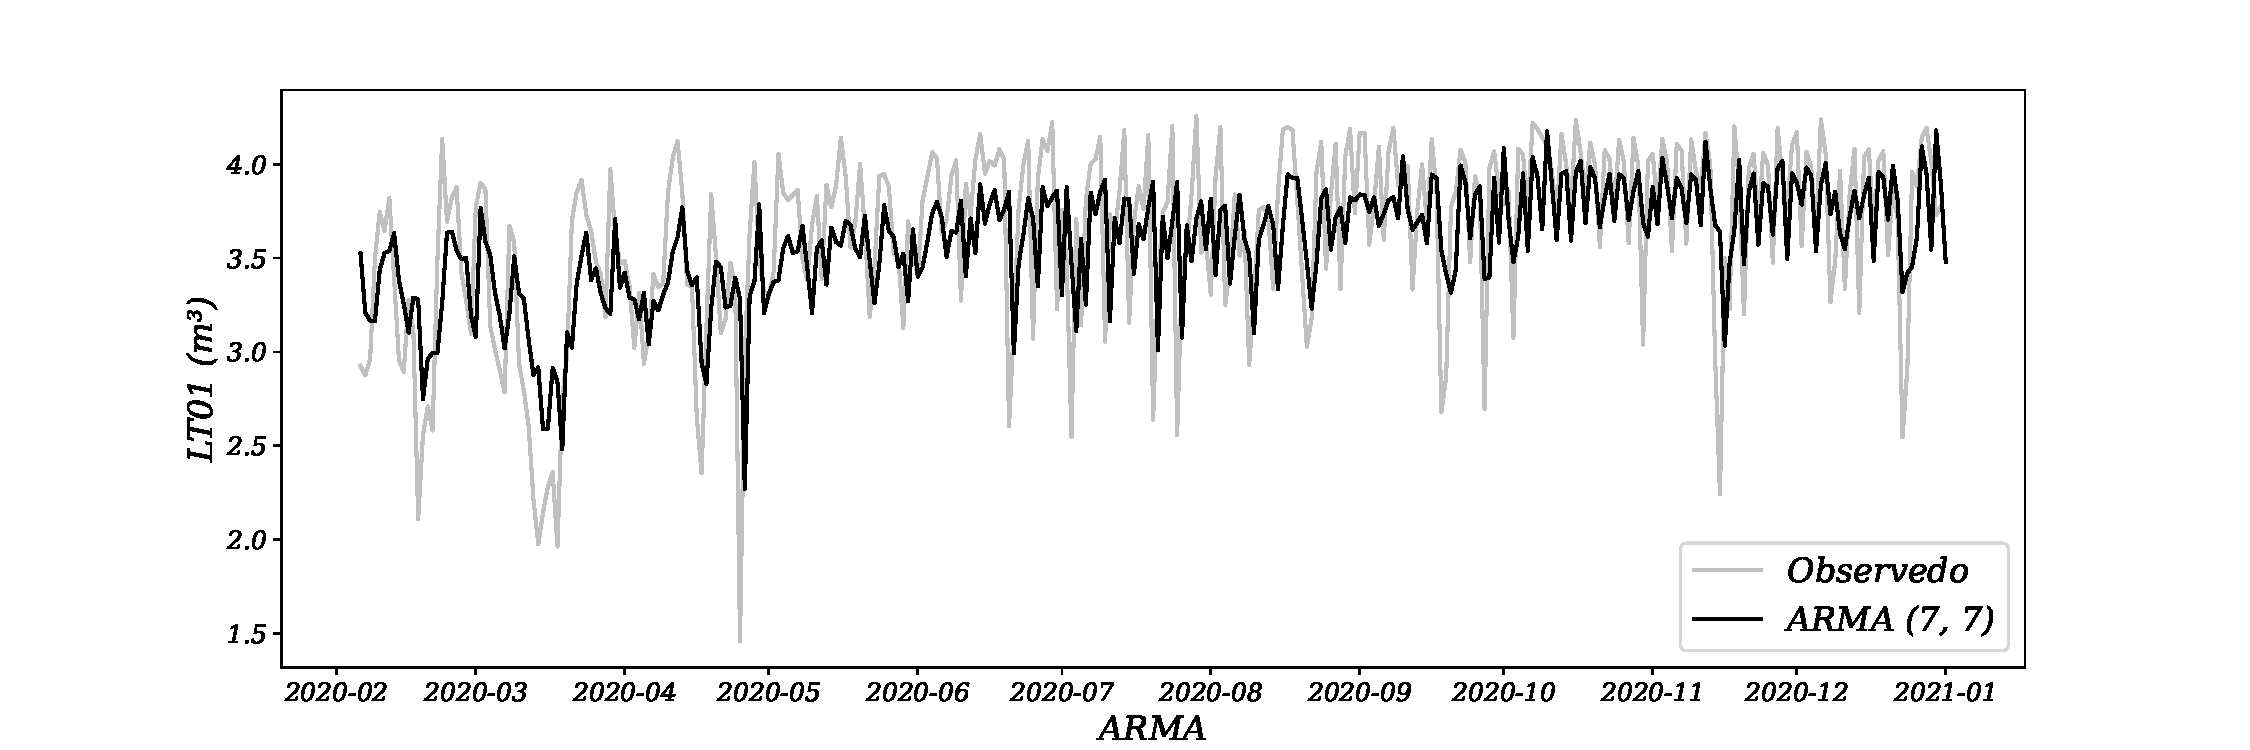
\includegraphics[width=1\linewidth]{Modelos/Figuras/ARMA}
	
	\fonte{Elaboração própria a partir de dados da SANEPAR (2018 a 2020)}
\end{figure}

A Figura \ref{fig:1-arma} ilustra a combinação dos modelos AR e MA em um modelo ARMA. Essa abordagem pode levar a uma redução significativa no erro de previsão, como observado nos apêndices \ref{sec:comtb24} e \ref{sec:comtb18}, onde são apresentadas comparações com um maior número de passos de previsão.

\subsubsection{ARIMA}

\begin{eqnarray}
	Y_t = \beta_2 + \omega_1\varepsilon_{t-1} + \omega_2 \varepsilon_{t-2} +\ldots+ \omega_q \varepsilon_{t-q} + \varepsilon_t \label{arima}
\end{eqnarray}

Na equação \eqref{arima}, a variável $Y_t$ representa a série temporal que foi diferenciada (possivelmente mais de uma vez). Os ``preditores'' no lado direito da equação incluem os valores defasados de $Y_t$ e os erros defasados. Esse tipo de modelo é conhecido como ARIMA ($p, d, q$).

O modelo ARIMA é uma extensão do modelo ARMA que incorpora uma etapa adicional de pré-processamento chamada de diferenciação. Essa etapa é representada pela notação \textbf{I(d)}, em que \textbf{d} denota a ordem de diferenciação, ou seja, o número de transformações necessárias para tornar a série temporal estacionária. Portanto, um modelo ARIMA é simplesmente um modelo ARMA aplicado à série temporal diferenciada. Isso permite lidar com séries temporais que possuem tendências ou padrões não estacionários.

\begin{figure}[!htb]
	\centering
	\caption{ARIMA (7,1,7)}
	\label{fig:1-arima}
	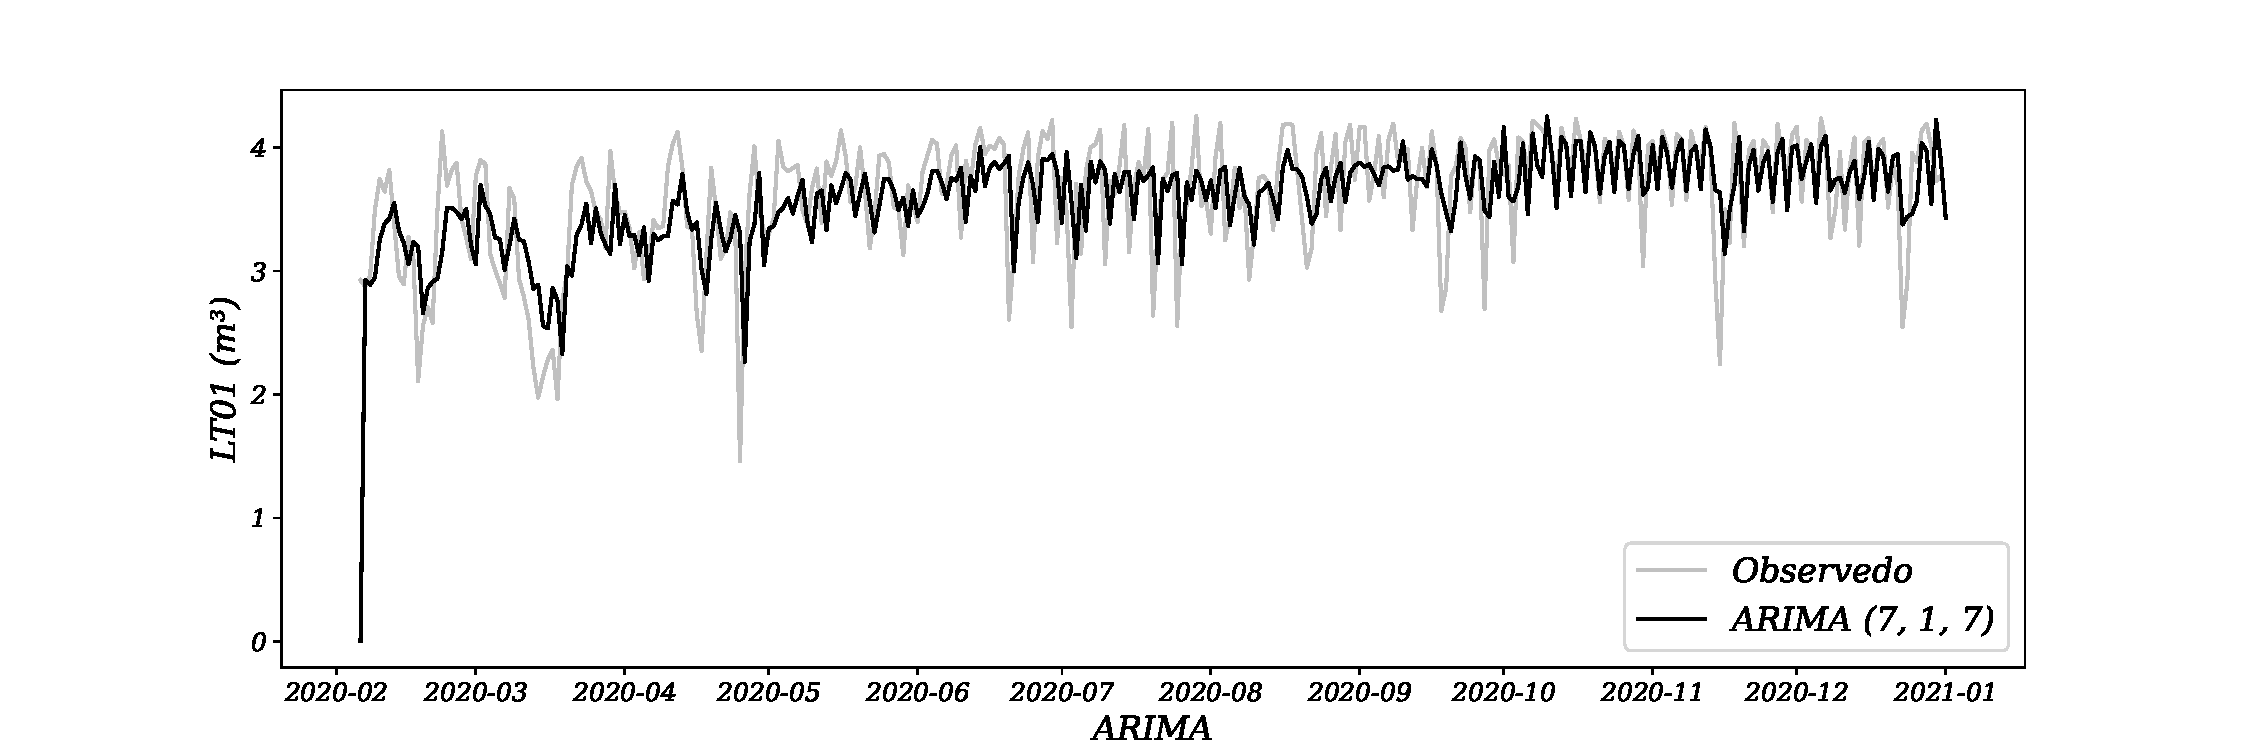
\includegraphics[width=1\linewidth]{Modelos/Figuras/ARIMA}
	
	Fonte: Elaboração própria a partir de dados da SANEPAR (2018 a 2020)
\end{figure}

Ao analisar a Figura \ref{fig:1-arima}, não se nota uma diferença visual significativa em relação aos outros métodos apresentados anteriormente. O método ARX ainda parece ser superior aos demais com base na análise visual.

Embora os modelos ARIMA sejam eficazes, incorporar variáveis sazonais e exógenas ao modelo pode potencializar sua capacidade de previsão. No entanto, é importante destacar que o modelo ARIMA pressupõe que a série temporal seja estacionária. Quando lidamos com séries temporais não estacionárias, é necessário recorrer a outros modelos para a análise e previsão adequadas.

\subsubsection{SARIMA}

\begin{eqnarray}
	Y_t&=&c+\sum_{n=1}^p \alpha_n y_{t-n}+\sum_{n=1}^q \theta_n \epsilon_{t-n}+\sum_{n=1}^P \phi_n y_{t-s n}+\sum_{n=1}^Q \eta_n \epsilon_{t-s n}+\epsilon_t \label{sarima}
\end{eqnarray}

O modelo proposto é uma extensão do modelo ARIMA, com a adição de componentes autorregressivos e de média móvel sazonal. Esses componentes extras são ajustados levando em consideração os padrões sazonais presentes nos dados, utilizando atrasos correspondentes à frequência sazonal (por exemplo, 12 para dados mensais). Essa abordagem permite capturar e modelar de forma mais precisa as variações sazonais e melhorar a qualidade das previsões em séries temporais com esse comportamento cíclico.

\begin{figure}[!htb]
	\centering
	\caption{SARIMA $(7,1,7) (2,1,1)_{12}$}
	\label{fig:1-sarima}
	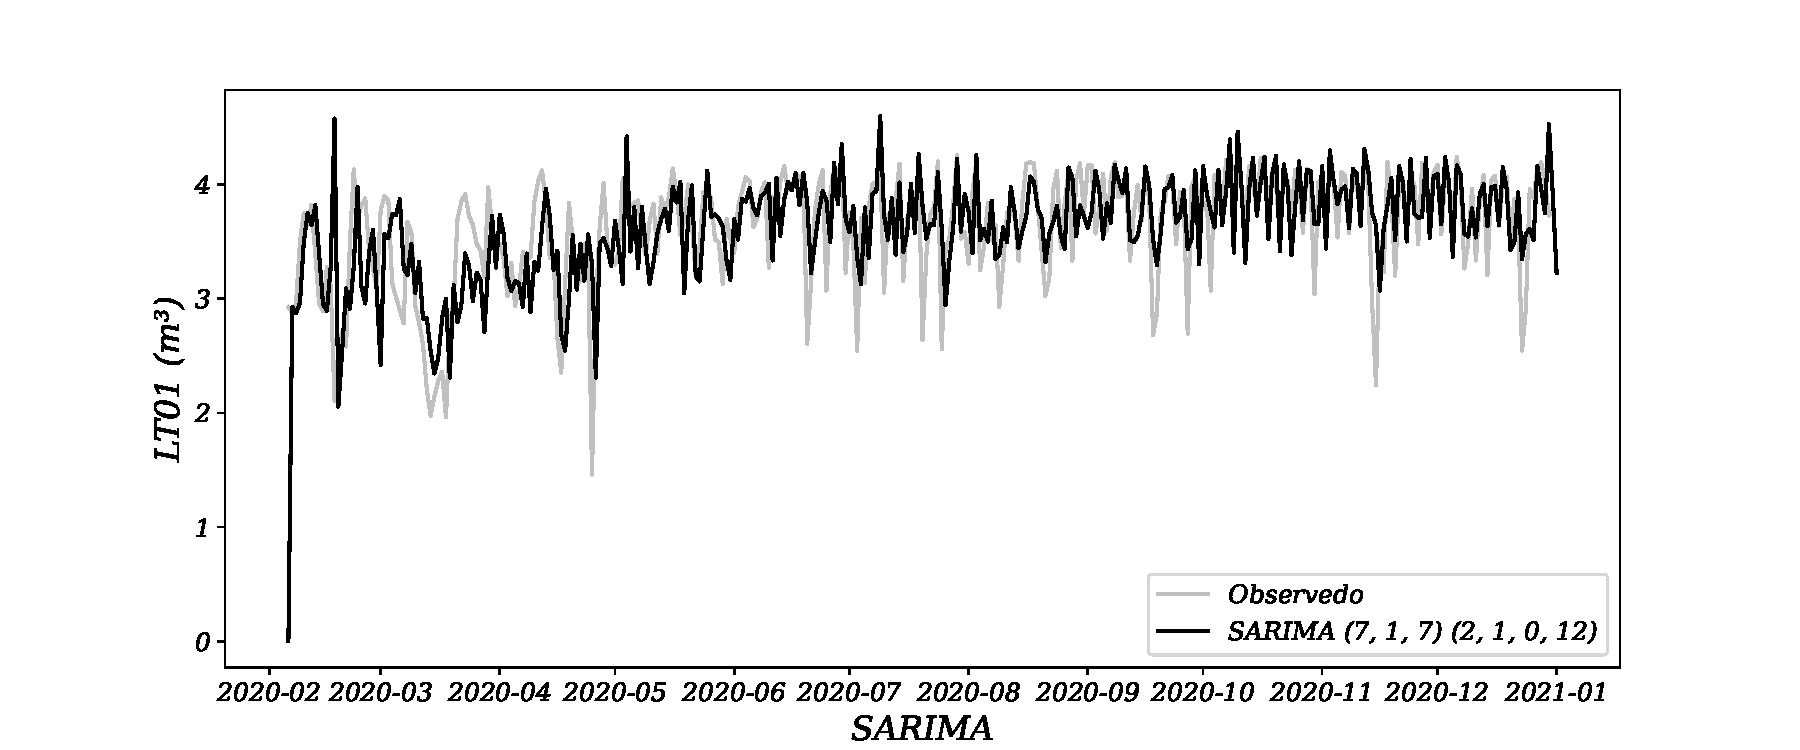
\includegraphics[width=1\linewidth]{Modelos/Figuras/SARIMA}
	
	\fonte{Elaboração própria a partir de dados da SANEPAR (2018 a 2020)}
\end{figure}

Na Figura \ref{fig:1-sarima}, é possível observar que a previsão em vermelho está mais próxima dos valores observados em preto, mostrando que a inclusão do componente de sazonalidade melhora a qualidade da previsão. Os modelos SARIMA são capazes de lidar com dados que apresentam padrões sazonais, permitindo a diferenciação dos dados em termos de componentes sazonais e não sazonais. Uma abordagem útil para determinar os melhores parâmetros do modelo é utilizar uma estrutura de pesquisa automatizada de parâmetros, como o pmdarima, que auxilia na identificação dos parâmetros ideais para o modelo SARIMA. Isso pode contribuir para uma melhor compreensão e ajuste do modelo aos dados observados.

\subsection{Modelos de S\'erie Temporal Multivariada}\label{subsec:mult}

Os Modelos de Série Temporal Multivariada são uma abordagem estatística utilizada para analisar e prever dados que possuem múltiplas variáveis dependentes ao longo do tempo. Nesse tipo de modelo, considera-se a interdependência entre as diferentes séries temporais, permitindo a análise conjunta e a identificação de padrões e relações entre as variáveis. Esses modelos são aplicados em diversas áreas, como economia, finanças, meteorologia e análise de dados, proporcionando insights valiosos para a compreensão e previsão de fenômenos complexos ao longo do tempo.

\subsubsection{ARIMAX e SARIMAX}

\begin{eqnarray}
	d_t=c+\sum_{n=1}^p \alpha_n d_{t-n}+\sum_{n=1}^q \theta_n \epsilon_{t-n}+\sum_{n=1}^r \beta_n x_{n_t}+\sum_{n=1}^P \phi_n d_{t-s n}+\sum_{n=1}^Q \eta_n \epsilon_{t-s n}+\epsilon_t \label{eq:sarmax}
\end{eqnarray}

Em \eqref{eq:sarmax}, o modelo SARIMAX é apresentado. Nesse modelo, são consideradas variáveis exógenas, ou seja, são utilizados dados externos para a realização das previsões. É importante ressaltar que mesmo que essas variáveis exógenas sejam indiretamente modeladas no histórico de previsões do modelo, ao incluí-las diretamente, o modelo será capaz de responder de forma mais ágil aos efeitos dessas variáveis. Isso significa que a incorporação de informações externas possibilita uma resposta mais rápida e precisa do modelo em relação aos fatores externos, resultando em previsões mais atualizadas e acuradas.

\begin{figure}[!htb]
	\centering
	\caption{Comparação entre ARIMAX e SARIMAX}
	\begin{subfigure}{1\textwidth}
		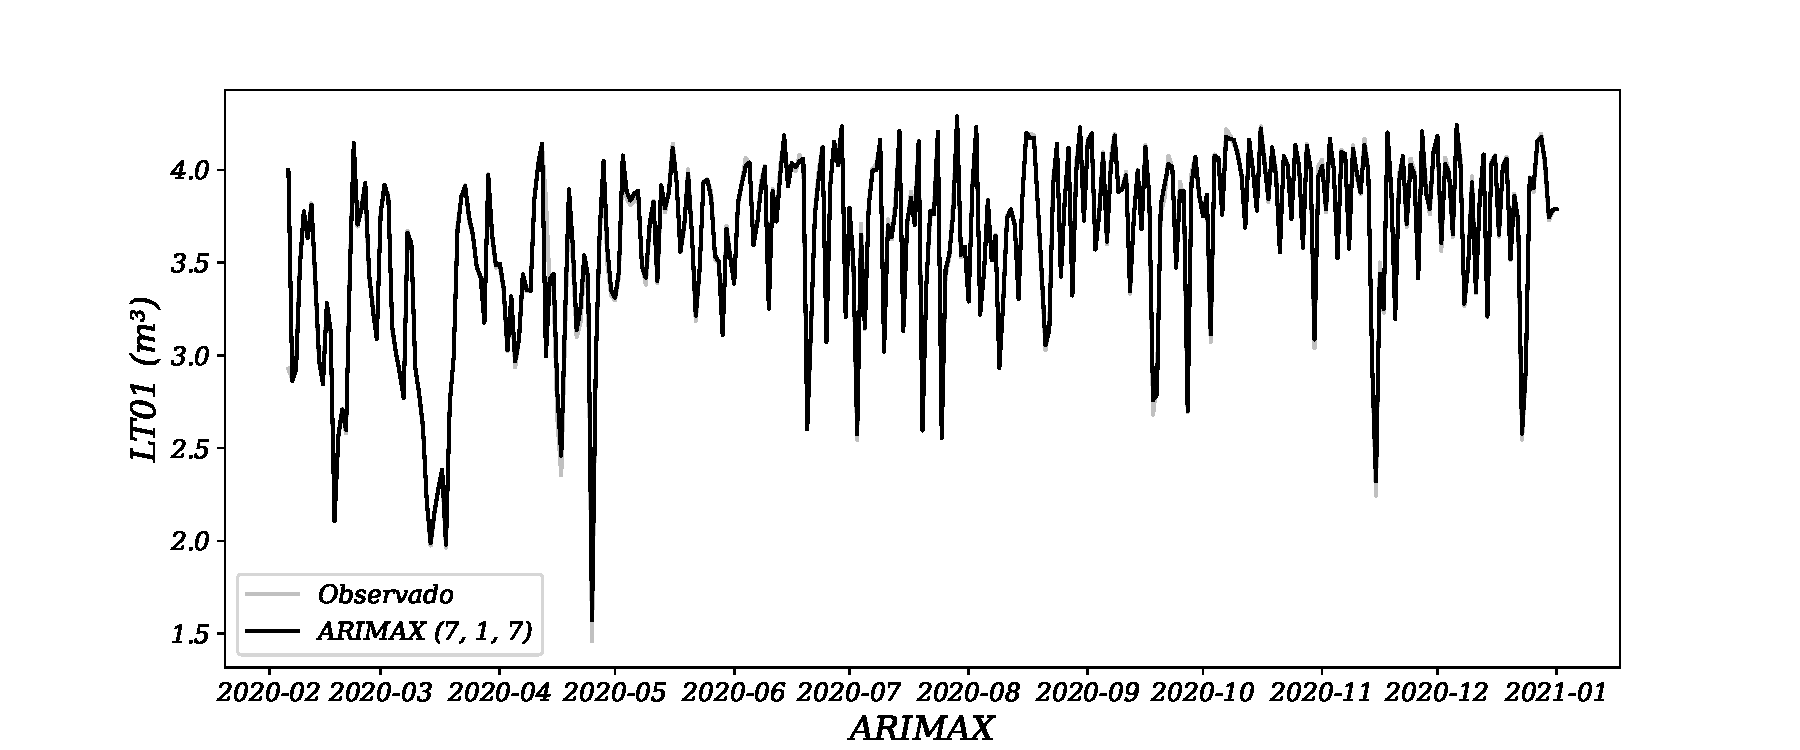
\includegraphics[width=\linewidth]{Modelos/Figuras/ARIMAX}
		\caption{ARIMAX $(7,1,7)$}
		\label{fig:1-arimax}
	\end{subfigure}
	\hfill
	
	\begin{subfigure}{1\textwidth}
		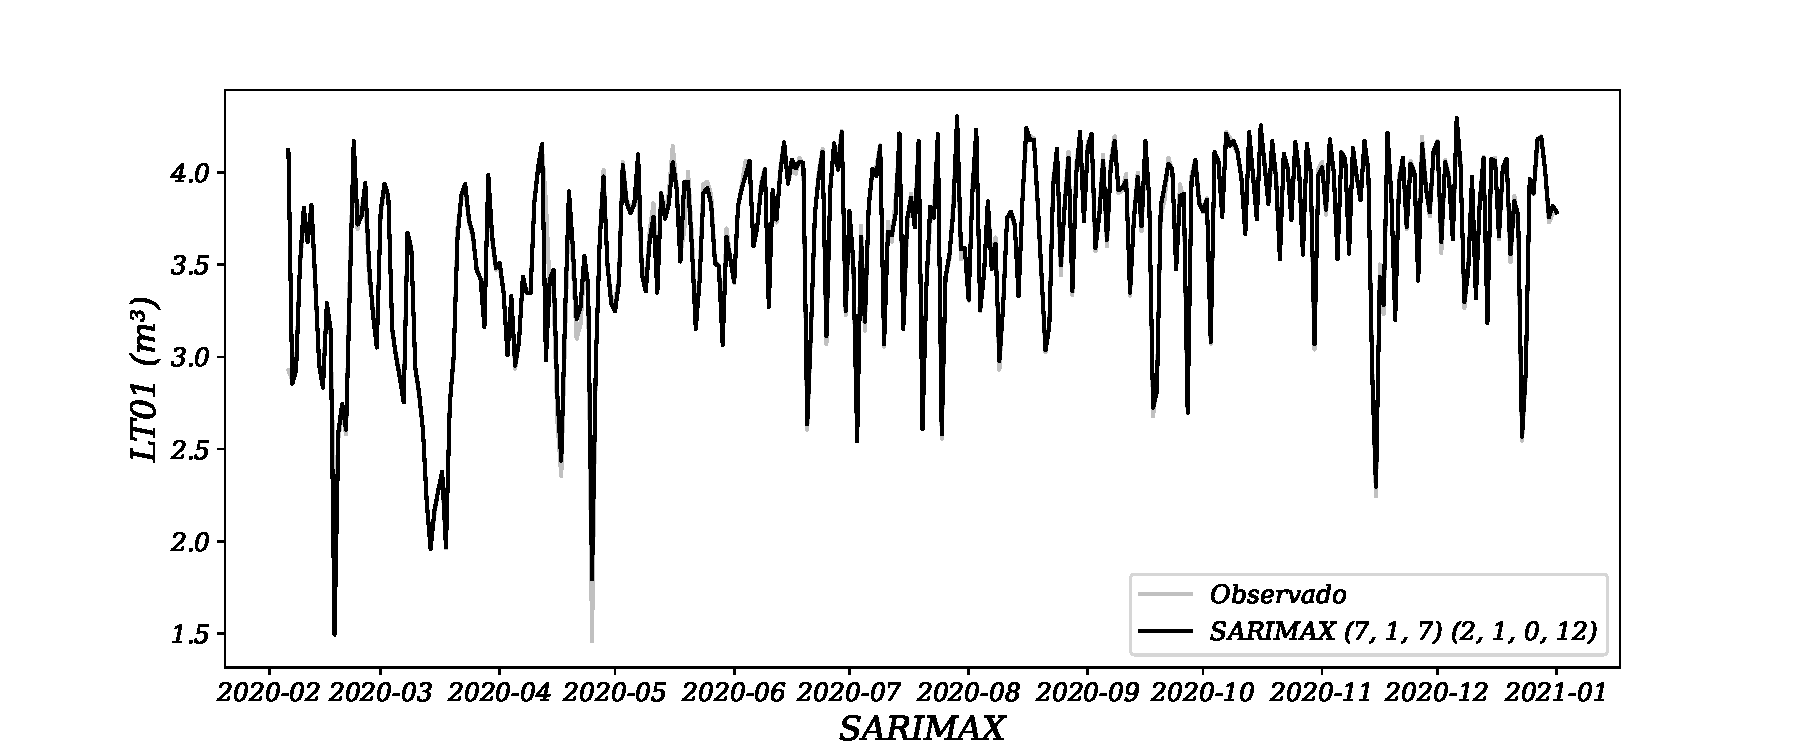
\includegraphics[width=\linewidth]{Modelos/Figuras/SARIMAX}
		\caption{SARIMAX $(7,1,7) (2,1,1)_{12}$}
		\label{fig:1-sarimax}	
	\end{subfigure}

		
	\fonte{Elaboração própria a partir de dados da SANEPAR (2018 a 2020)}
\end{figure}


Entre os modelos com variáveis exógenas, como mostrado nas Figuras \ref{fig:1-arimax} e \ref{fig:1-sarimax}, observa-se uma melhora significativa na qualidade das previsões em comparação com os modelos que não incluem variáveis exógenas. A adição dessas variáveis externas permite capturar melhor as influências e os padrões presentes nos dados, resultando em previsões mais completas e precisas. Essa inclusão de informações adicionais contribui para uma compreensão mais abrangente do comportamento da série temporal e possibilita uma melhor adaptação do modelo aos padrões observados.


\subsection{Modelos de Aprendizado de M\'aquina Supervisionados}\label{subsec:reg}

Os modelos regressivos para séries temporais têm sido amplamente reconhecidos e utilizados na literatura atual, especialmente aqueles baseados em métodos de gradiente. Esses modelos, incluindo a regressão linear simples, têm se destacado como uma escolha popular em competições de séries temporais em todo o mundo.

Esses modelos são valorizados por sua capacidade de capturar relações complexas e não lineares nos dados, permitindo previsões mais precisas e eficientes. Sua popularidade reflete o reconhecimento da eficácia desses modelos em abordar uma ampla gama de problemas de previsão de séries temporais em diferentes áreas de estudo.

A abordagem regressiva, combinada com técnicas de otimização baseadas em gradiente, tem se mostrado particularmente eficaz na obtenção de resultados de alta qualidade. Esses modelos são capazes de aprender a partir dos dados históricos e ajustar seus parâmetros de forma iterativa, otimizando assim o desempenho da previsão.

Com a crescente disponibilidade de dados e avanços na área de aprendizado de máquina, espera-se que os modelos regressivos para séries temporais continuem a evoluir e desempenhar um papel importante na análise e previsão de dados temporais em diversas aplicações.

\subsubsection{Regress\~ao Linear (LR)}

De acordo com o estudo realizado por \citeonline{korstanje2021}, nos modelos de aprendizado de máquina supervisionados, é feita uma tentativa de identificar as relações existentes entre diferentes variáveis:


\begin{itemize}
	\item Variável de destino: a variável que você tenta prever
	\item Variáveis explicativas: Variáveis que ajudam você a prever o alvo variável
\end{itemize}

Para realizar previsões, é importante que se compreenda quais tipos de variáveis explicativas podem ser utilizadas. Neste exemplo, a variável \textbf{Pressão de Sucção (PT01SU)} será considerada como a variável $x$, enquanto a variável \textbf{Nível do Reservatório (Câmara 1) LT01} será considerada como a variável $y$, com base na análise de correlação de Pearson ilustrada na Figura \ref{fig:person}. O coeficiente de correlação indica a relação entre o eixo $x$ e $y$, como expresso pela seguinte fórmula.



A fórmula do coeficiente de correlação de Pearson é dada por:

\begin{equation}
	r=\frac{\sum\left(x_i-\bar{x}\right)\left(y_i-\bar{y}\right)}{\sqrt{\left(\sum\left(x_i-\bar{x}\right)^2\right)\left(\sum\left(y_i-\bar{y}\right)^2\right)}}
\end{equation}

Onde $x_i$ e $y_i$ representam os valores das variáveis $X$ e $Y$, respectivamente. $\bar{x}$ e $\bar{y}$ são as médias dos valores $x_i$ e $y_i$. O coeficiente de correlação de Pearson mede a força e a direção da relação linear entre as variáveis $X$ e $Y$. Valores próximos a 1 indicam uma correlação positiva forte, valores próximos a -1 indicam uma correlação negativa forte, e valores próximos a 0 indicam uma ausência de correlação entre as variáveis.

\begin{figure}[H]
	\centering
	\caption{Corelação de Pearson}
	\label{fig:person}
	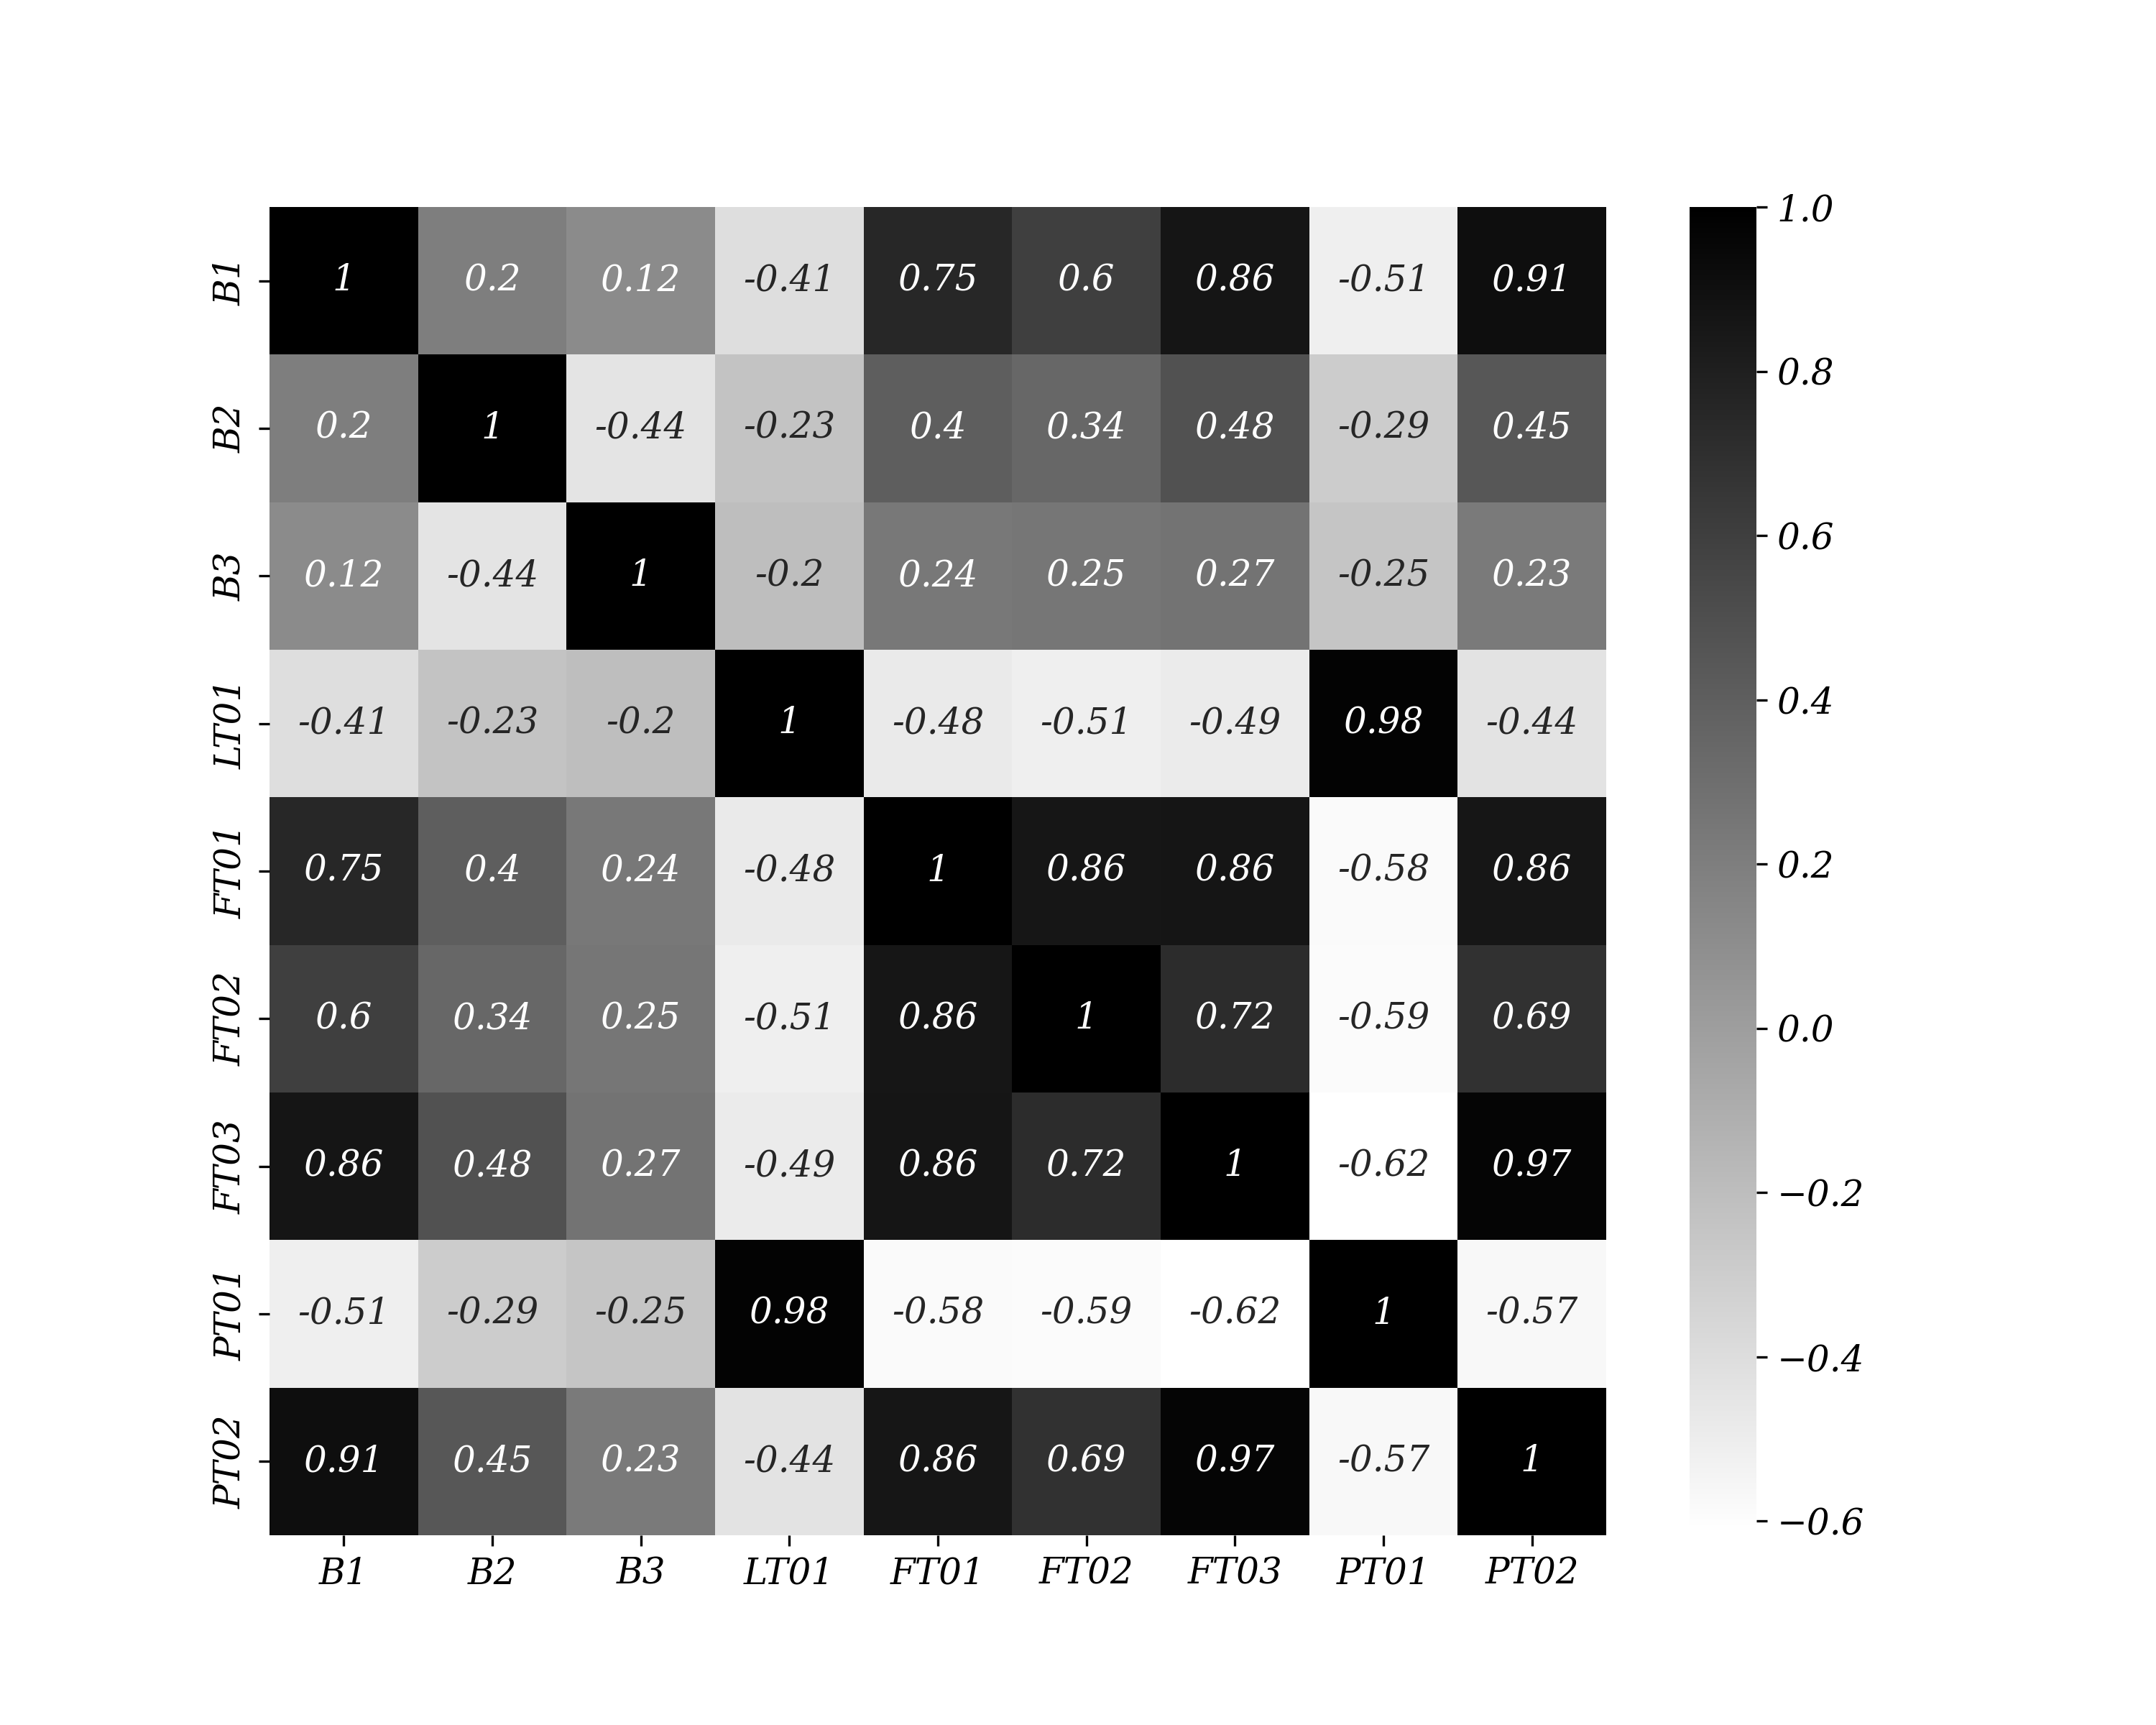
\includegraphics[width=0.9\linewidth]{Apendices/Figuras/modelagem-24h/person}
	
	Fonte: Elaboração própria a partir de dados da SANEPAR (2018 a 2020)
\end{figure}

A Figura \ref{fig:person} ilustra a correlação entre as variáveis no conjunto de dados em questão. Essa imagem representa graficamente a relação entre as variáveis e é usada para demonstrar a existência de uma correlação forte entre elas. Com base nessa análise, é possível responder à pergunta de pesquisa \ref{q1}, pois a correlação entre as variáveis é significativa.

\subsubsection{Defini\c c\~ ao do modelo}

A regressão linear é definida da seguinte forma:

\begin{equation}
	y = \beta_0 + \beta_1 x_1 + \cdots + \beta_p x_p + \varepsilon \label{eq:lr}
\end{equation}

Da Equação \eqref{eq:lr}, temos as seguintes variáveis:

\begin{itemize}
	\item Há $p$ variáveis explicativas, denotadas por $x$.
	\item Existe uma variável alvo, denotada por $y$.
	\item O valor de $y$ é calculado como uma constante $\beta_0$, somada aos valores das variáveis $x$ multiplicados por seus coeficientes $\beta_1$ a $\beta_p$.
\end{itemize}

\begin{figure}[H]
	\centering
	\caption{Regressão linear LT01 vs PT01 correlação 98\%}
	\label{fig:lr-lt01-m3}
	\includegraphics[width=0.9\linewidth]{"Modelos/Figuras/LR LT01 (m³)"}
	
	Fonte: Elaboração própria a partir de dados da SANEPAR (2018 a 2020)
\end{figure}



A Figura \ref{fig:lr-lt01-m3} fornece uma representação visual da interpretação dos coeficientes $\beta_0$ e $\beta_1$. Ela ilustra que um aumento de $1$ na variável $x$ está associado a um aumento proporcional de $\beta_1$ na variável $y$. O valor de $\beta_0$ representa o valor de $y$ quando $x$ é igual a $0$.

Para utilizar a regressão linear, é necessário estimar os coeficientes (betas) com base em um conjunto de dados de treinamento. Esses coeficientes podem ser estimados por meio da seguinte fórmula, expressa em notação matricial:

\begin{eqnarray}
	\hat{\beta}&=&\left(X^T X\right)^{-1} X^T y\label{eq:ols}
\end{eqnarray}

A fórmula mencionada, conhecida como \textbf{OLS} (método dos mínimos quadrados ordinários), é amplamente utilizada na regressão linear \citeonline{korstanje2021}. Esse método é conhecido por ser rápido de ajustar, pois requer apenas cálculos matriciais para estimar os coeficientes $\beta$. No entanto, ele é mais adequado para processos lineares e pode ser menos adequado para modelos mais complexos que envolvam relações não-lineares. Portanto, é importante considerar suas limitações ao aplicar a regressão linear em contextos mais complexos.

\begin{figure}[H]
	\centering
	\caption{Regressão linear (LR) um passo a frente}
	\label{fig:1-regressao-linear}
	\includegraphics[width=0.9\linewidth]{Modelos/Figuras/0-regressão-linear}
	
	Fonte: Elaboração própria a partir de dados da SANEPAR (2018 a 2020)
\end{figure}


\subsubsection{Floresta Aleat\'oria (Random Forest)} \label{subsubsec:rf}

Pode-se observar que ter exatamente a mesma árvore de decisão repetidas vezes não adiciona valor significativo em comparação a usar essa mesma árvore de decisão apenas uma vez. Em modelos de conjunto, cada modelo individual deve ser ligeiramente diferente dos demais. Existem dois métodos amplamente reconhecidos para criar conjuntos: o ensacamento (\textit{bagging}) e o reforço (\textit{boosting}). A floresta aleatória utiliza o ensacamento para criar um conjunto de árvores de decisão, onde cada árvore é construída com uma amostra aleatória do conjunto de dados original. Isso garante que as árvores sejam distintas e diversificadas, contribuindo para a robustez e eficácia do modelo.


\begin{figure}[H]
	\centering
	\caption{Regressão da Floresta Aleatória (RFR)}
	\label{fig:1-regressao-rfa}
	\includegraphics[width=0.9\linewidth]{Modelos/Figuras/0-regressão-rfa}
	
	Fonte: Elaboração própria a partir de dados da SANEPAR (2018 a 2020)
\end{figure}


Segundo \citeonline{Pelletier2016156}, cada árvore em um modelo de Floresta Aleatória de Regressão (RFR) é construída por meio de um algoritmo de aprendizado individual que divide o conjunto de variáveis de entrada em subconjuntos, com base em um teste de valor de atributo, como o coeficiente de Gini. Ao contrário das árvores de decisão clássicas, as árvores de RFR são construídas sem poda e selecionam aleatoriamente um subconjunto de variáveis de entrada em cada nó. Atualmente, o número de variáveis utilizadas para dividir um nó em uma RFR (denotado por $m$) corresponde à raiz quadrada do número total de variáveis de entrada. Essa abordagem ajuda a aumentar a diversidade das árvores e aprimorar o desempenho do modelo.

\begin{figure}[H]
	\centering
	\caption{Esquema da Floresta Aleatória}
	\label{fig:rf}
	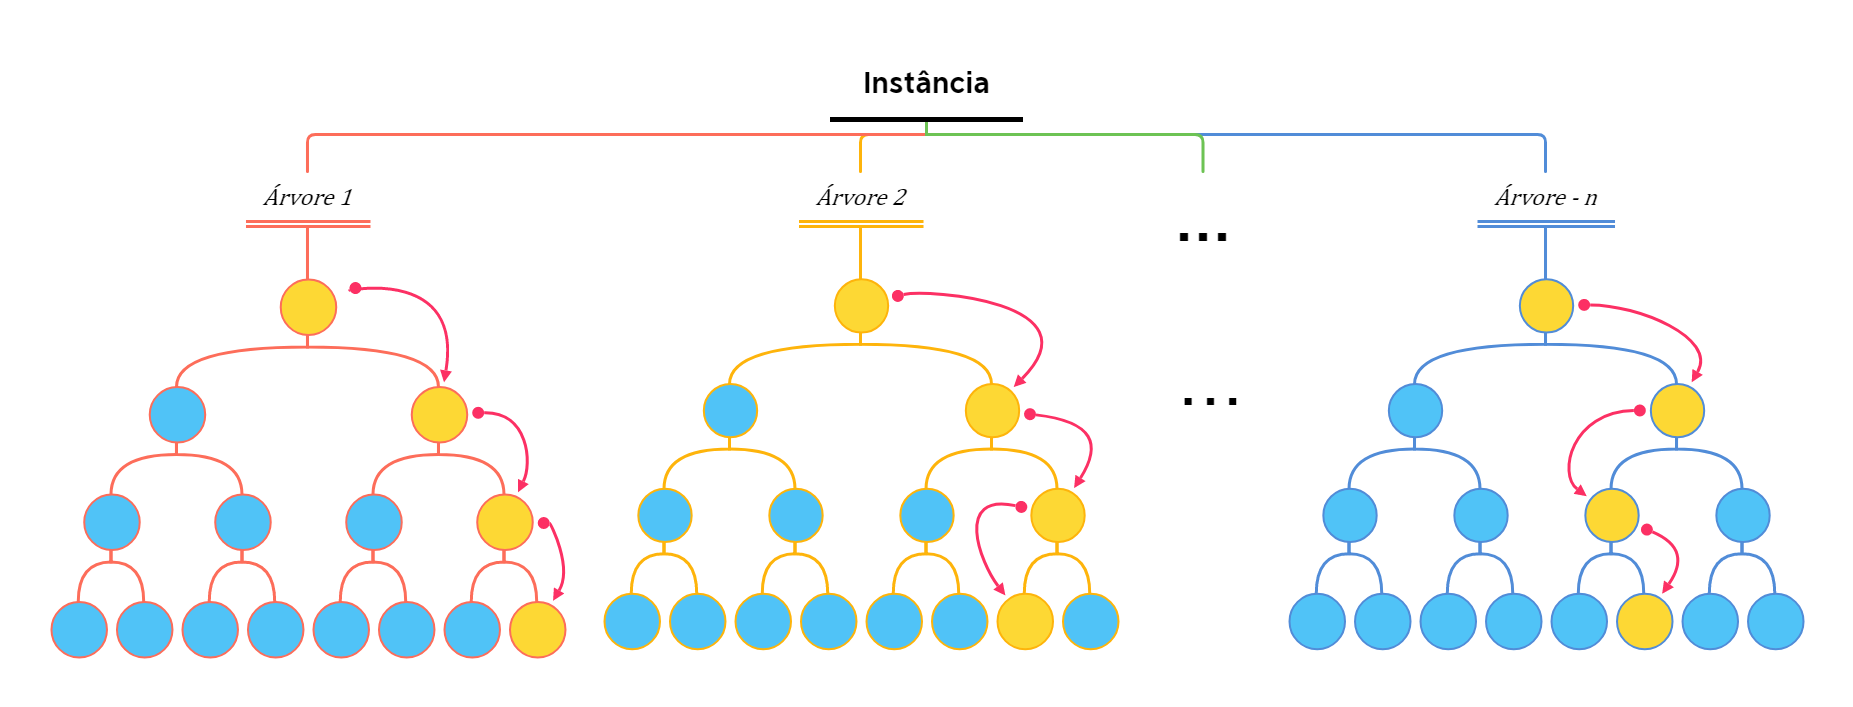
\includegraphics[width=0.9\linewidth]{Modelos/Figuras/RF}
	
	Fonte: Elaboração própria
\end{figure}


\subsubsection{Gradient Boosting (como XGBoost, LightGBM)}\label{subsubsec:lgbxgb}

O aumento de gradiente (do inglês\textit{gradient boosting}) é um método que combina vários modelos de árvore de decisão para realizar previsões. Cada uma dessas árvores de decisão é única, pois a diversidade é um elemento importante nesse processo. A diversidade é alcançada através de um processo chamado boosting, que é uma abordagem iterativa. O boosting adiciona modelos fracos ao conjunto de forma inteligente, dando mais peso aos pontos de dados que ainda não foram bem previstos. 

O processo de boosting melhora o conjunto ao focar nas partes dos dados que ainda não são compreendidas. A Figura \ref{fig:xgboost} apresenta uma visão esquemática desse processo. À medida que novos modelos fracos são adicionados, todos os modelos fracos intermediários são mantidos. O modelo final é uma combinação de todos esses modelos fracos, resultando em um ensemble que oferece uma melhor capacidade de previsão do que um único modelo.

O boosting é apenas um dos métodos de ensemble utilizados em conjunto com o bagging. O bagging também é um método que utiliza múltiplos modelos de árvore de decisão, porém, em vez de adicionar os modelos de forma iterativa, cada modelo é treinado independentemente em subconjuntos aleatórios dos dados de treinamento. Ambos os métodos, boosting e bagging, têm como objetivo melhorar o desempenho do modelo combinando as previsões de múltiplos modelos individuais.


\begin{figure}[H]
	\centering
	\caption{Impulsionando gradiente com XGBoost e LightGBM}
	\label{fig:xgboos}
	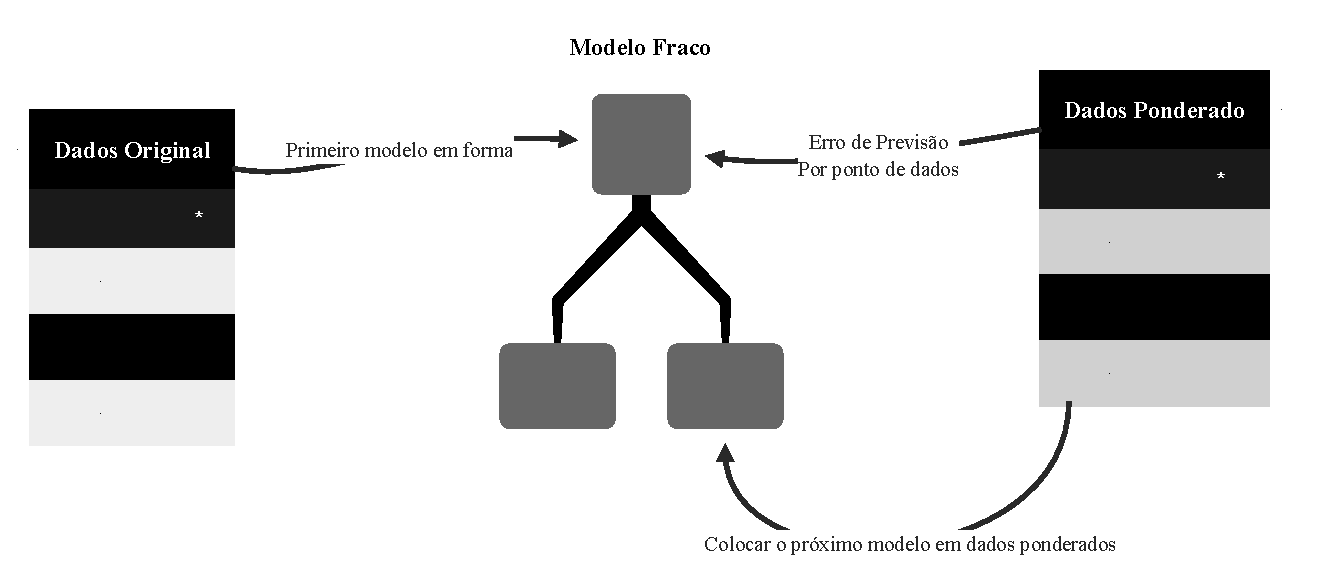
\includegraphics[width=0.9\linewidth]{Modelos/Figuras/xgboos}
	
	Fonte: Adaptação de \citeonline{korstanje2021}
\end{figure}



\subsubsection{O Gradiente em Gradiente de Boosting (Refor\c co)} \label{subsubsec:boosting}

O processo iterativo utilizado no aumento de gradiente, como descrito por \citeonline{korstanje2021}, recebe esse nome por um motivo. O termo ``gradiente'' refere-se a um campo vetorial de derivadas parciais que apontam na direção da inclinação mais acentuada. De forma simplificada, podemos pensar nos gradientes como as inclinações das estradas: quanto maior a inclinação, mais íngreme a colina. Para calcular os gradientes, são realizadas derivadas ou derivadas parciais de uma função.

No aumento de gradiente, ao adicionar árvores adicionais ao modelo, o objetivo é incorporar uma árvore que explique melhor a variação que ainda não foi explicada pelas árvores anteriores. Dessa forma, a nova árvore tem como objetivo ajustar-se aos erros ou resíduos deixados pelas árvores anteriores.

\begin{equation}
	y-\hat{y} \label{eq:xb}
\end{equation}

A equação \eqref{eq:xb} pode ser reescrita como a derivada parcial negativa da função de perda em relação às previsões $\hat{y}$:

\begin{equation}
	y-\hat{y} = -\frac{\partial L}{\partial \hat{y}} \label{eq:xb2}
\end{equation}

Isso é definido como o objetivo da nova árvore a ser adicionada no modelo de aumento de gradiente, garantindo que ela explique a máxima quantidade de variação adicional no modelo geral. Essa é a razão pela qual o modelo é chamado de "aumento de gradiente" (``\textit{gradient boosting}'', em inglês). O processo utiliza o gradiente da função de perda para guiar a adição de novas árvores, buscando minimizar o erro e melhorar a capacidade do modelo em explicar a variação nos dados.

\subsubsection{Algoritmos de boosting de gradiente}

Existem muitos algoritmos que executam versões ligeiramente diferentes de aumento de gradiente. Quando o método de aumento de gradiente foi inventado, o algoritmo não tinha um desempenho tão bom, mas isso mudou com o advento do algoritmo AdaBoost: o primeiro algoritmo capaz de se adaptar a modelos fracos.

O algoritmo de aumento de gradiente é uma das ferramentas de aprendizado de máquina com melhor desempenho no mercado. Após o AdaBoost, uma longa lista de algoritmos de aumento levemente diferentes foi adicionada à literatura, incluindo XGBoost, LightGBM, LPBoost, BrownBoost, MadaBoost, LogitBoost e TotalBoost. Ainda há muitas contribuições para melhorar a teoria do aumento de gradiente. Nesta subseção, dois algoritmos são apresentados: XGBoost e LightGBM.

O \textbf{XGBoost} é um dos algoritmos de aprendizado de máquina mais utilizados. É uma forma rápida de obter bom desempenho. Devido à sua facilidade de uso e alto desempenho, é frequentemente o primeiro algoritmo escolhido por muitos profissionais de aprendizado de máquina.

O \textbf{LightGBM} é outro algoritmo de aumento de gradiente que é importante conhecer. Atualmente, é um pouco menos difundido que o XGBoost, mas está ganhando popularidade rapidamente. A vantagem esperada do LightGBM em relação ao XGBoost é um ganho de velocidade e uma utilização mais eficiente de memória.

Nesta subseção, você encontrará as implementações de ambos os algoritmos de aumento de gradiente.

\subsubsection{A diferen\c ca entre XGBoost e LightGBM}

Se alguém planeja utilizar os dois algoritmos de aumento de gradiente, é importante que essa pessoa compreenda suas diferenças, o que também proporciona uma visão das várias divergências que existem entre os modelos disponíveis no mercado.

Uma diferença fundamental reside na maneira como esses algoritmos identificam as melhores divisões entre os nós das árvores de decisão individuais. É crucial lembrar que uma divisão em uma árvore de decisão ocorre quando a árvore precisa encontrar a separação que mais melhora o desempenho do modelo.

A abordagem intuitiva e simples para encontrar a melhor divisão é iterar por todas as possibilidades e selecionar a melhor. No entanto, essa abordagem é computacionalmente custosa, e algoritmos mais recentes apresentam alternativas mais eficientes.

Uma alternativa proposta pelo XGBoost é a segmentação baseada em histograma. Nesse caso, em vez de iterar por todas as partições possíveis, o modelo constrói um histograma para cada variável e utiliza-os para encontrar a melhor divisão geral entre as variáveis.

O LightGBM, desenvolvido pela Microsoft, adota uma abordagem mais eficiente para a definição das divisões. Essa abordagem é conhecida como amostragem unilateral baseada em gradiente (GOSS). O GOSS calcula o gradiente para cada ponto de dados e utiliza-o para filtrar os pontos de dados com gradientes baixos. Afinal, os pontos de dados com gradientes baixos já são bem compreendidos, enquanto aqueles com gradientes altos precisam ser melhor aprendidos.

O LightGBM também utiliza uma abordagem chamada Exclusive Feature Bundling (EFB), que acelera a seleção de muitas variáveis correlacionadas. Outra diferença é que o modelo LightGBM é adequado para o crescimento de folhas (leaf-wise growth), enquanto o XGBoost cultiva as árvores em níveis (level-wise growth). Essa diferença pode ser visualizada na Figura \ref{fig:xgboost}.

Essa diferença teoricamente favorece o LightGBM em termos de precisão, mas também apresenta um maior risco de overfitting (sobreajuste) quando há poucos dados disponíveis. Portanto, é importante que a pessoa considere essas distinções ao escolher entre os dois algoritmos de aumento de gradiente.

\begin{figure}[H]
	\centering
	\caption{Crescimento em folha versus crescimento em nível}
	\label{fig:xgboost}
	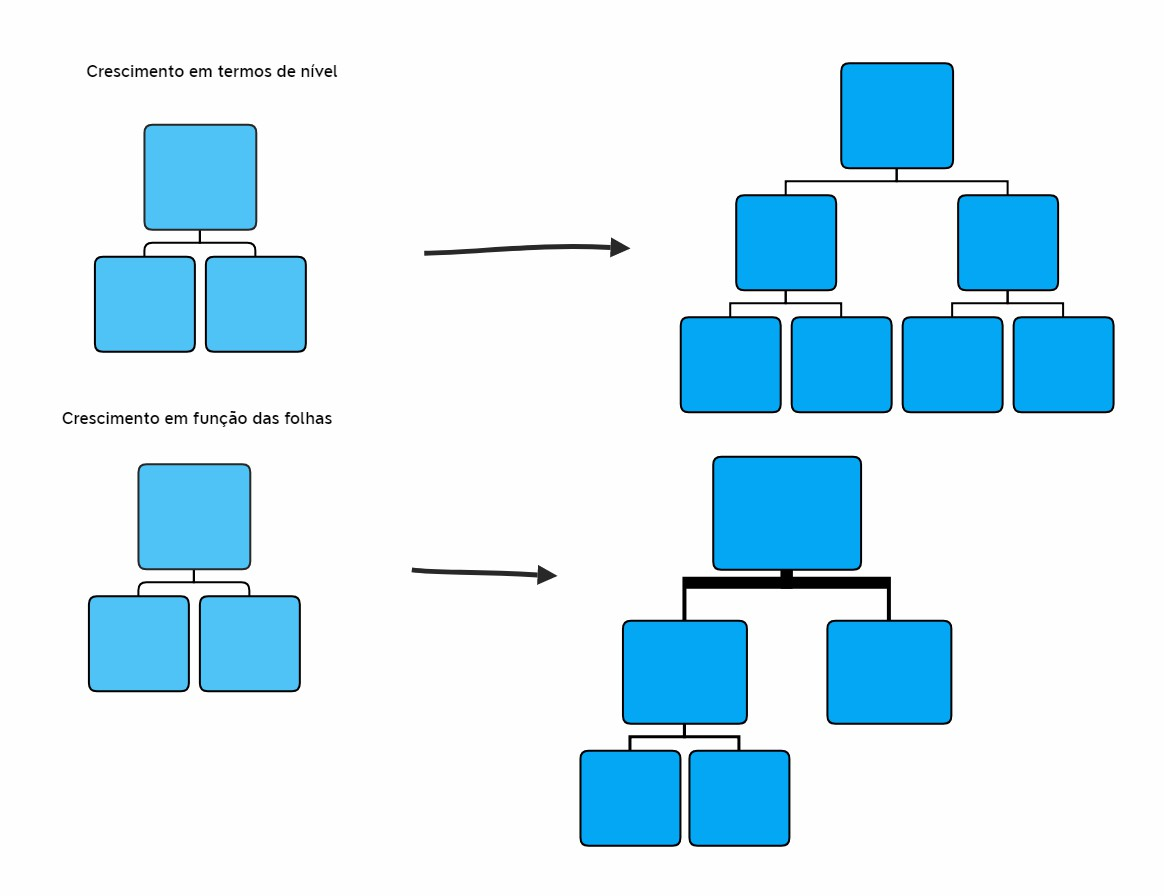
\includegraphics[width=0.9\linewidth]{Modelos/Figuras/xgboost}
	
	Fonte: Adaptação de \citeonline{korstanje2021}
\end{figure}


Na Figura \ref{fig:xgboost}, é possível visualizar como cada modelo é ajustado durante o processo de crescimento de árvore em folhas e em níveis. Essa representação gráfica oferece uma compreensão visual das diferenças entre os dois métodos.

No crescimento de árvore em folhas, como no LightGBM, novas folhas são adicionadas à árvore de forma iterativa, visando maximizar a redução do erro de treinamento. Isso significa que as árvores são expandidas adicionando folhas, uma a uma, até que o critério de parada seja alcançado.

Por outro lado, no crescimento em níveis, como no XGBoost, as árvores são expandidas em profundidade de forma simultânea em todos os níveis. Ou seja, em cada nível, todas as folhas são expandidas ao mesmo tempo, resultando em um crescimento mais uniforme da árvore.

Essa distinção no modo de crescimento das árvores pode afetar o comportamento e o desempenho do modelo. Portanto, compreender essa diferença é importante ao escolher entre esses algoritmos de aumento de gradiente.

\begin{figure}[H]
	\centering
	\caption{XGBoost e LigthGBM regressão}\label{fig:1-xgb-regressao}
	\includegraphics[width=0.9\linewidth]{Modelos/Figuras/0-xgb-regressão}
	
\end{figure}

\begin{figure}[H]
	\centering
	\includegraphics[width=0.9\linewidth]{Modelos/Figuras/0-lgbm-regressão}	
	
	
	Fonte: Elaboração própria a partir de dados da SANEPAR (2018 a 2020)
	
\end{figure}

Na Figura \ref{fig:1-xgb-regressao} é um modelo baseado nos dados coletados da SANEPAR.



\subsection{M\'etricas de Avalia\c c\~ao de Modelos}\label{subsec:metrica}

A métrica de Erro Quadrático Médio (MSE) é amplamente utilizada no campo do aprendizado de máquina para avaliar a qualidade dos modelos de previsão. O MSE é calculado pela média da soma dos quadrados das diferenças entre os valores reais e os valores previstos,

\begin{eqnarray}
	MSE &=& \frac{1}{n} \sum_{i=1}^{n} (y_i - \hat{y}_i)^2 \label{eq:mse}
\end{eqnarray}

\noindent onde, $n$ representa o número de amostras, $y_i$ é o valor real correspondente à amostra $i$ e $\hat{y}_i$ é o valor previsto para a mesma amostra. O MSE é calculado como a média das diferenças ao quadrado entre os valores reais e os valores previstos.

A utilização do MSE fornece uma medida quantitativa da precisão do modelo, pois penaliza de forma mais significativa os erros maiores. Ao elevar as diferenças ao quadrado, a métrica enfatiza a importância de minimizar as discrepâncias entre os valores reais e os valores previstos. Dessa forma, quanto menor o valor do MSE, melhor é o desempenho do modelo em termos de previsão.

Portanto, o MSE é uma métrica fundamental para avaliar a qualidade dos modelos de previsão e é amplamente utilizada para comparar diferentes algoritmos e abordagens de aprendizado de máquina.

\subsubsection{Erro Quadr\'atico M\'edio Raiz (RMSE)}

O RMSE é uma métrica amplamente empregada na avaliação de modelos de previsão em séries temporais. Ele é calculado tomando a raiz quadrada do MSE, conforme segue,

\begin{eqnarray}
	RMSE &=& \sqrt{\dfrac{1}{n} \sum_{i=1}^{n} (y_i - \hat{y}_i)^2} \label{eq:rmse}
\end{eqnarray}

\noindent onde \eqref{eq:rmse}, $n$ representa o número de amostras, $y_i$ é o valor real correspondente à amostra $i$, e $\hat{y}_i$ é o valor previsto para a mesma amostra. O RMSE fornece uma medida da dispersão média entre os valores reais e os valores previstos pelo modelo.

Uma das vantagens de utilizar o RMSE é que, ao computar a raiz quadrada, o erro passa a ter a mesma escala da variável de interesse. Isso permite uma interpretação mais fácil dos resultados, sendo que um valor baixo de RMSE indica um bom desempenho do modelo, já que o erro se aproxima de zero.

O RMSE possui algumas características positivas. Ele penaliza de forma significativa os valores discrepantes, caso seja necessário para o modelo. Além disso, o erro resultante está nas mesmas unidades da série temporal, facilitando a interpretação. O RMSE pode ser considerado uma combinação das melhores características do MSE e do Erro Absoluto Médio (MAE).

No entanto, o RMSE também apresenta algumas desvantagens. Ele tem uma interpretabilidade reduzida, uma vez que os erros ainda são elevados ao quadrado. Além disso, o RMSE é dependente da escala dos dados, o que impede sua comparação direta com modelos de séries temporais que utilizam unidades diferentes.

Apesar das limitações, o RMSE é uma métrica amplamente utilizada para avaliar modelos de previsão em séries temporais. Ele fornece uma medida da dispersão média entre os valores reais e previstos, auxiliando na compreensão do desempenho do modelo e na comparação com outras abordagens.

\subsubsection{Raiz do Erro M\'edio Quadr\'atico Relativo (RRMSE)}\label{subsub:rrmse}

\noindent\textbf{Vantagens do RRMSE :}


Interpretação intuitiva: O RRMSE é expresso como uma porcentagem, o que facilita a compreensão da precisão relativa do modelo. Quanto menor o valor do RRMSE, mais próximas estão as previsões dos valores reais.
	
Considera a escala dos dados: O RRMSE leva em consideração a magnitude dos erros em relação aos valores de referência. Isso é especialmente útil quando os dados têm uma grande variação e escala, pois evita que erros de grande magnitude dominem a avaliação.
	
Comparação entre modelos e algoritmos: O RRMSE pode ser usado para comparar a precisão de diferentes modelos ou algoritmos em um problema de regressão. Ao calcular o RRMSE para cada modelo, é possível identificar aquele que apresenta melhor desempenho em relação aos valores reais.
	
Sensibilidade relativa a diferentes magnitudes de erro: O RRMSE captura erros relativos em diferentes magnitudes. Isso significa que ele é capaz de identificar discrepâncias proporcionais, independentemente do valor absoluto dos erros.


\noindent\textbf{Desvantagens do RRMSE:}


Sensibilidade a \textit{outliers}: O RRMSE pode ser influenciado por valores discrepantes nos dados. Se houver valores extremos que não representem a tendência geral, o RRMSE pode ser distorcido, pois considera a média dos valores reais na fórmula de cálculo.
	
Necessidade de uma linha de base adequada: O RRMSE requer uma linha de base apropriada para comparação. Isso significa que é necessário ter um valor de referência confiável ou um modelo de referência para calcular o RRMSE e interpretar os resultados corretamente.
	
Foco exclusivo na precisão relativa: O RRMSE se concentra exclusivamente na precisão relativa e não leva em consideração outras métricas de desempenho, como tempo de execução, complexidade do modelo ou outros aspectos específicos do problema em questão. Portanto, é importante complementar o uso do RRMSE com outras métricas relevantes,





\begin{eqnarray}
	\text{RRMSE} &=& \left(\frac{\text{RMSE}}{\text{Média dos Valores Reais}}\right) \times 100 \label{eq:rrmse}
\end{eqnarray}


\noindent onde RMSE representa o Erro Médio Quadrático e ``Média dos Valores Reais'' denota a média aritmética dos valores reais no conjunto de dados.

É essencial que sejam consideradas essas vantagens e desvantagens ao utilizar o RRMSE como métrica de avaliação. Além disso, é recomendado o uso de várias métricas em conjunto para obter uma visão mais completa do desempenho do modelo de regressão.



\subsubsection{Erro Absoluto M\'edio (MAE)}

O Erro Absoluto Médio (MAE) é amplamente utilizado como uma métrica para avaliar o desempenho de modelos de previsão. Em vez de calcular a média das diferenças entre os valores reais e previstos, o MAE calcula a média dos valores absolutos dessas diferenças, garantindo que os erros positivos e negativos não se anulem.

O MAE mede o desvio médio das previsões em relação aos valores reais e é uma métrica intuitiva e fácil de interpretar, representando a magnitude média dos erros em relação à escala dos dados. Por exemplo, um MAE de 2 significa que, em média, as previsões têm um desvio absoluto de 2 unidades em relação aos valores reais.

Uma das vantagens do MAE é a sua insensibilidade a valores extremos, pois trata os erros de forma absoluta. No entanto, como o MAE não considera a magnitude dos erros individuais, pode não refletir adequadamente a gravidade de desvios significativos em relação aos valores reais.

Para superar essa limitação, uma alternativa é o Erro Médio Absoluto Percentual (MAPE). O MAPE expressa o MAE como uma porcentagem em relação aos valores reais, proporcionando uma medida relativa de erro. Essa métrica é especialmente útil quando se deseja avaliar o desempenho de um modelo em relação à magnitude dos dados.

Em resumo, o MAE é uma métrica simples e fácil de interpretar, que mede o desvio médio das previsões em relação aos valores reais. O MAPE, por sua vez, fornece uma medida relativa de erro, expressa como uma porcentagem dos valores reais. A escolha entre essas métricas depende do contexto do problema e dos requisitos específicos de avaliação.

O cálculo do MAE é realizado utilizando o valor absoluto da diferença entre o valor real e o valor previsto, e em seguida, divide-se pela quantidade $n$ de amostras. Isso resulta no erro médio absoluto. A equação do MAE é dada por:

\begin{eqnarray}
	M A E &=& \dfrac{1}{n} \sum\left|y_i-\hat{y}_i\right|\label{eq:mae}
\end{eqnarray}

Sua interpretação é similar ao RMSE, em que o erro é expresso na mesma escala ou ordem de grandeza da variável estudada.

\subsubsection{Erro Percentual Absoluto M\'edio (MAPE)}

O Erro Percentual Absoluto Médio (MAPE) é uma métrica que expressa o erro de previsão como uma porcentagem relativa ao valor observado. Ele é calculado somando as diferenças entre o valor real e o valor previsto (representando o erro), dividido pelo valor observado.
O MAPE é calculado usando a seguinte fórmula:

\begin{eqnarray}
	MAPE &=& \dfrac{1}{n} \sum\left|\frac{y_i - \hat{y}_i}{y_i}\right|\label{eq:mape}
\end{eqnarray}

No entanto, surge um problema quando o valor observado $y_i$ é igual a zero, pois é matematicamente impossível dividir por zero. O MAPE é uma medida de erro em que valores menores indicam um melhor desempenho de previsão.
Uma alternativa ao MAPE é calcular $1 - \text{MAPE}$, que representa a porcentagem de acerto.
O Erro Percentual Absoluto Médio é comumente usado como uma métrica de referência para avaliar o desempenho de modelos de previsão.

\noindent\textbf{Vantagens do MAPE:}


Fácil de interpretar.
Independente de escala, permitindo comparações entre diferentes séries temporais


\noindent\textbf{Desvantagens do MAPE:}

Erro infinito se o valor real estiver próximo ou igual a zero.
Previsões mais baixas estão propensas a ter um erro de 100\%, enquanto previsões mais altas podem ter um erro infinito, o que resulta em um viés de subprevisão.
Essa métrica são amplamente utilizadas na avaliação de modelos de previsão em diferentes áreas e ajudam a quantificar a qualidade das previsões realizadas pelos modelos.

\subsubsection{Erro Percentual Absoluto M\'edio Sim\'etrico (sMAPE)}


O sMAPE (do inglês \textit{Symmetric Mean Absolute Percentage Error}), ou Erro Médio Percentual Absoluto Simétrico, é outra métrica comumente utilizada para avaliar a precisão de modelos de previsão. Aqui estão as vantagens e desvantagens do sMAPE:

\noindent\textbf{Vantagens do sMAPE:}


Interpretação intuitiva: O sMAPE é expresso como uma porcentagem, facilitando a compreensão da precisão relativa do modelo. Valores menores indicam uma melhor precisão.	
Simetria: Ao contrário do MAPE (do inglês \textit{Mean Absolute Percentage Error}), o sMAPE é simétrico em relação aos valores previstos e reais. Isso significa que ele considera igualmente as discrepâncias de subestimação e superestimação.	
Robustez contra valores nulos: O sMAPE é adequado para lidar com valores nulos nos dados, pois a divisão por zero é evitada no cálculo da métrica.


\noindent\textbf{Desvantagens do sMAPE:}


Sensibilidade a valores extremos: O sMAPE é sensível a valores extremos nos dados. Se houver valores discrepantes que não representem a tendência geral, eles podem influenciar significativamente a métrica.	
Assimetria em torno de zero: Embora o sMAPE seja simétrico em relação aos valores previstos e reais, ele não é simétrico em torno de zero. Isso pode causar interpretações inconsistentes, especialmente quando os valores reais são próximos de zero.



\begin{eqnarray}
	sMAPE &=& \dfrac{1}{n} \sum_{i=1}^{n} \dfrac{2|y_i - \hat{y}_i|}{(|y_i| + |\hat{y}_i|)} \times 100\label{eq:smape}
\end{eqnarray}


\noindent onde $y_i$ representa o valor real, $\hat{y}_i$ representa o valor previsto e $n$ é o número total de amostras.
Ao utilizar o sMAPE como métrica de avaliação, é importante considerar esses prós e contras. Além disso, recomenda-se o uso de várias métricas em conjunto para obter uma visão abrangente do desempenho do modelo de previsão.






\subsection{Trabalhos Relacionados}\label{subsec:estudo-de-caso-base}


A previsão da demanda de água é uma preocupação fundamental para muitas organizações e autoridades responsáveis pelo abastecimento de água. A análise de séries temporais é uma abordagem comumente usada para prever padrões futuros com base em dados históricos. Neste estudo de caso, será explorado como a análise de séries temporais pode ser aplicada para prever a demanda de água ao longo do tempo.



Na subseção \ref{subsubsec:obespec} estão as perguntas de pesquisa que serão abordadas no estudo de caso, da pergunta \ref{q1} à \ref{q5}, com as ramificações da \ref{q5}.
Na subseção \ref{subsec:descricao}, são apresentadas as variáveis contidas no conjunto de dados coletado no período de $2018$ a $2020$, durante uma grave falta de água que afetou a cidade. Devido a essa situação, foi implementado um rodízio de abastecimento de água para os residentes. Os dados foram coletados em intervalos de uma hora, levando em consideração cada variável, com ênfase na variável-alvo, denominada LT01, que representa o nível do reservatório.

O conjunto de dados possui um total de $26.306$ linhas e $9$ colunas. Durante a coleta dos dados, verificou-se que eles apresentam padrões sazonais, indicando variações recorrentes ao longo do tempo. Além disso, constatou-se que o consumo diário foi significativamente afetado no ano de 2020, diferindo dos anos anteriores, nos quais as mudanças não foram tão significativas.

Ao longo do trabalho realizado, pôde-se observar na subseção \ref{subsec:detec} que foi realizada uma análise gráfica do problema antes da aplicação de qualquer método. A detecção de anomalias mostrou-se desafiadora, porém não impossível de ser realizada. Essa detecção permitiu a análise da presença de sazonalidade nos dados. A decomposição STL foi utilizada para essa finalidade, conforme descrito na etapa \ref{etp:3} e detalhado na subseção \ref{subsubsec:stl}, onde são apresentadas as decomposições realizadas.

É fundamental lembrar que, durante a análise exploratória, os dados sofreram algumas alterações. Por exemplo, a média diária foi calculada em vez de ser considerada a nível horário, resultando em uma redução do conjunto de dados de 26.306 linhas para 1.096 linhas. A decomposição STL foi aplicada nos formatos aditivo e multiplicativo, e ambas as abordagens estão ilustradas nas Figuras \ref{fig:stl-aditiva} e \ref{fig:stl}, respectivamente.
Adicionalmente, na subseção \ref{subsubsec:stl}, foi realizada a verificação da estacionariedade da série. O teste de DF (do inglês \textit{Dickey-Fuller}) foi empregado para auxiliar na tomada de decisões, e os resultados demonstraram que a série em análise é estacionária, conforme evidenciado pelo teste DF.


Dentro da análise, foram incluídos uma variedade de modelos para melhor capturar a natureza dos dados e aprimorar as previsões. Esses modelos incluem:
RNN, que leva em conta as dependências sequenciais nos dados para prever valores futuros.
LSTM, um tipo de RNN que lida especialmente bem com sequências longas e dependências de longo prazo.
GRU, outra variante de RNN que equilibra o poder de modelagem e a eficiência computacional.
Transformer, um modelo amplamente utilizado para tarefas de processamento de linguagem natural e sequências, que também pode ser adaptado para previsões sequenciais.
Prophet, um modelo de previsão desenvolvido pelo Facebook que lida bem com dados sazonais e tendências.
\textit{Decision Tree Regressor}, um modelo baseado em árvore de decisão que segmenta os dados em subgrupos para fazer previsões.
Esses modelos são complementados com abordagens tradicionais como:

Modelos de séries temporais univariados, incluindo AR, MA, ARMA, ARIMA e SARIMA, que levam em consideração a sazonalidade dos dados.
Modelos de séries temporais multivariados, como ARX, ARIMAX e SARIMAX, que incorporam variáveis exógenas para melhorar as previsões.
Foram explorados modelos de aprendizado de máquina supervisionados:

LR (\textit{Regressão Linear}), que estabelece relações lineares entre variáveis para fazer previsões.
RFR (\textit{Random Forest Regressor}), um \textit{ensemble} de árvores de decisão que captura complexas relações nos dados.
LightGBM e XGBoost, modelos baseados em \textit{gradient boosting} que são reconhecidos por sua eficácia na previsão e tomada de decisões. O XGBoost é particularmente conhecido por seu desempenho superior em várias métricas de avaliação.



\noindent\textbf{Ajuste do modelo}


Ao ajustar o modelo para a base de dados, foi feita uma alteração na ordem do modelo sugerido pelo \textbf{pmdarima}. A escolha foi trocar o modelo SARIMAX(1,1,1)(2,1,0,12) para SARIMAX(7,1,7)(2,1,0,12). Essa decisão foi tomada com base na observação de um ajuste mais preciso aos dados, evidenciado pela redução nos resíduos e uma melhor captura das características da série temporal. Além disso, considerando o conhecimento do problema e as características específicas dos dados, foi identificado que padrões mais complexos requeriam ordens mais altas para serem adequadamente capturados. Dessa forma, foi realizado um processo iterativo de experimentação e avaliação para determinar o modelo SARIMAX(7,1,7)(2,1,0,12) como o mais adequado para a base de dados em questão. É importante ressaltar que o desempenho do novo modelo será avaliado por meio de diagnósticos adicionais e análise dos resultados obtidos.

Os modelos RNN, LSTM e GRU foram ajustados minuciosamente por meio da técnica de otimização de hiperparâmetros do Optuna, permitindo uma exploração adaptativa e eficiente do espaço de configurações. Essa abordagem exclusiva do Optuna resultou em modelos sequenciais com aprimoramento notável na capacidade preditiva. Parâmetros vitais, como taxa de aprendizado, tamanho da camada oculta e número de unidades, foram otimizados de forma eficaz através do Optuna \cite{DBLP}.

O RFR apresentou melhorias notáveis após o ajuste com o Optuna. A otimização realizada pelo Optuna permitiu identificar uma combinação de hiperparâmetros ideal para o RFR, resultando em um significativo aprimoramento no desempenho preditivo desse modelo.
Considerando que o modelo LR não demonstrou melhorias significativas, uma decisão foi tomada para substituí-lo pelo modelo \textit{Decision Tree Regressor}. Este último foi ajustado empregando o Optuna, buscando encontrar a configuração de hiperparâmetros ideal para o modelo de árvore de decisão. Essa decisão foi respaldada pelo fato de que o Optuna havia demonstrado ser uma ferramenta eficaz para otimização de hiperparâmetros, como evidenciado pelas melhorias observadas no RFR e em outros modelos \cite{DBLP}.

Dessa forma, os modelos RNN, LSTM, GRU, XGBRegressor, LGBMRegressor e o Decision Tree Regressor foram todos otimizados com sucesso utilizando o Optuna, resultando em previsões mais robustas e confiáveis. No entanto, os modelos Transformer e Prophet mantiveram suas configurações originais devido à ausência de melhorias substanciais após tentativas de otimização com o Optuna.

O \textbf{Optuna} oferece uma abordagem de otimização de hiperparâmetros mais avançada e eficaz em comparação com outras técnicas amplamente utilizadas, como o GridSearchCV, BayesSearchCV e RandomizedSearchCV. Enquanto essas abordagens tradicionais têm suas vantagens, o Optuna leva a otimização de hiperparâmetros a um nível superior.
Existem geralmente dois tipos de métodos de amostragem: a amostragem relacional, que explora as correlações entre os parâmetros, e a amostragem independente, que recolhe amostras de cada parâmetro de forma independente. A amostragem independente não é necessariamente uma opção ingênua, porque alguns algoritmos de amostragem como o TPE A eficácia em termos de custos da amostragem relacional e independente depende do ambiente e da tarefa. O Optuna apresenta ambos, e pode lidar com vários métodos de amostragem independente independentes, incluindo TPE, bem como métodos de amostragem relacional como o CMA-ES. No entanto, há que ter algumas palavras de precaução para a implementação da amostragem relacional num definido por execução \cite{DBLP}.

\noindent\textbf{Avalia\c c\~ao do modelo}


A avaliação da precisão dos modelos de previsão é uma etapa fundamental no processo de modelagem. Diversas métricas podem ser utilizadas para esse propósito, como o sMAPE, o MAE e o RRMSE. Essas métricas têm sido amplamente adotadas na literatura de previsão e são consideradas indicadores confiáveis para mensurar a qualidade das previsões.

O MAPE é uma métrica bastante utilizada na avaliação de modelos de previsão, especialmente quando há variações significativas nos dados ou quando se deseja comparar a precisão de diferentes modelos. O MAPE calcula o erro médio percentual entre as previsões e os valores reais, fornecendo uma medida relativa da precisão do modelo \cite{zhang2016}.
O uso do erro médio absoluto (MAE) apresenta vantagens na avaliação do desempenho médio de um modelo, em comparação com o erro quadrático médio (RMSE) \cite{willmott2005advantages}.
Destacam a importância do RMSE na avaliação de modelos e argumentam contra a exclusão dessa métrica na literatura \cite{jones2017}.


O RRMSE é uma métrica de avaliação altamente eficaz para medir a precisão relativa de modelos de regressão. Eles destacam que sua normalização em relação à média dos valores reais permite uma interpretação intuitiva e facilita a comparação entre diferentes modelos. Segundo os autores, o RRMSE é amplamente utilizado na literatura devido à sua capacidade de fornecer uma medida robusta e padronizada da precisão dos modelos de regressão \cite{lopes2020evaluation}. O MAPE é amplamente utilizado na avaliação de modelos de previsão, especialmente quando há variações significativas nos dados ou quando se deseja comparar a precisão de diferentes modelos \cite{peng2017effective}.

O sMAPE é uma métrica amplamente utilizada para avaliar a precisão de modelos de previsão. Eles afirmam que o sMAPE possui algumas vantagens, como a consideração da simetria dos erros percentuais e a interpretação intuitiva como uma medida de precisão relativa \cite{nguyen2020toxicological}.

O MAE e o RMSE são métricas amplamente adotadas na análise de previsões, pois fornecem uma medida direta do desvio absoluto e do desvio quadrático médio entre as previsões e os valores observados. O MAE é particularmente útil quando se busca uma medida de erro que não seja sensível a valores extremos, enquanto o RMSE penaliza de forma mais significativa os erros maiores, oferecendo uma visão mais abrangente da precisão do modelo \cite{jones2017}.

O sMAPE é uma métrica de avaliação popular para comparar a precisão de diferentes modelos de previsão. Eles destacam que o sMAPE é particularmente útil quando os valores de demanda têm diferentes magnitudes, pois captura os erros relativos em uma escala percentual. Além disso, o sMAPE possui uma interpretação intuitiva e facilita a comparação entre modelos de previsão \cite{hyndman2006effect}.

\subsubsection{Estudo de Caso 1}

\noindent\textbf{Estudo de Caso 1: Adequação da Pressão e Vazão em uma Rede de Distribuição de Água}

\eqref{q1} Adequação da pressão atual para atender à demanda diária: Neste estudo de caso, o modelo SARIMAX (H) foi utilizado para avaliar a adequação da pressão atual em uma rede de distribuição de água, considerando a demanda diária \cite{2-s2.0-85099424908}. O objetivo foi prever a pressão na rede com base em dados históricos, permitindo que fosse realizada uma análise crítica da capacidade do sistema em atender às necessidades dos consumidores.

\eqref{q2} Volume mínimo de água no reservatório para evitar o acionamento das bombas: Para determinar o volume mínimo de água necessário no reservatório para evitar o acionamento das bombas durante o horário de pico, foi empregado um modelo Decision Tree Regressor (I) \cite{2-s2.0-85054695177}. Este modelo ajudou a identificar regras e padrões que guiam a tomada de decisão sobre o nível de armazenamento ideal.

\eqref{q3} Vazão ótima para atender à demanda diária: O estudo também buscou encontrar a vazão ótima para atender à demanda diária. Para isso, utilizou-se o modelo XGBRegressor (K) para otimizar a vazão na rede de distribuição, considerando as flutuações na demanda ao longo do dia \cite{2-s2.0-85130441623}.

\subsubsection{Estudo de Caso 2}

\noindent\textbf{Estudo de Caso 2: Impacto do Acionamento das Bombas durante o Horário de Pico em uma Rede de Distribuição de Água}

\eqref{q5} Impacto do acionamento das bombas durante o horário de pico: Neste segundo estudo de caso, analisou-se o impacto do acionamento das bombas durante o horário de pico em uma rede de distribuição de água.

\ref{q5}\eqref{q5:a} Nível ideal no reservatório e variação das vazões nos horários críticos: Utilizou-se o modelo ARIMA (E) \cite{2-s2.0-85069459067} para prever o nível ideal no reservatório e analisar as variações das vazões nos horários críticos, levando em consideração as diferentes estações do ano.

\ref{q5}\eqref{q5:b} Tendência, padrão e sazonalidade nos dados do Bairro Alto: Para identificar tendências, padrões e sazonalidades nos dados de três anos do Bairro Alto, empregou-se o modelo de decomposição STL, reconhecido por sua eficácia na modelagem de séries temporais com essas características.

\ref{q5}\eqref{q5:c} Identificação dos horários de maior demanda: A identificação dos horários de maior demanda entre as 18h e as 21h foi realizada com o uso da RNN (P) \cite{2-s2.0-85067419084}.

\ref{q5}\eqref{q5:d} Tendência, padrão e sazonalidade nos dados do Bairro Alto: Para identificar tendências, padrões e sazonalidades nos dados de três anos do Bairro Alto, empregou-se o modelo decomposição STL, reconhecido por sua eficácia na modelagem de séries temporais com essas características. Volume de armazenamento no reservatório para evitar o acionamento das bombas: Determinar a quantidade de água a ser armazenada previamente no reservatório para evitar o acionamento das bombas durante o horário de pico envolveu o modelo LGBMRegressor (L).

\ref{q5}\eqref{q5:e} Tendência, Padrão e Sazonalidade nos Dados do Bairro Alto: Para identificar tendências, padrões e sazonalidades nos dados de três anos do Bairro Alto, empregou-se o modelo STL, reconhecido por sua eficácia na modelagem de séries temporais com essas características. Detecção de anomalias na rede com base no histórico): Para detectar anomalias na rede com base no histórico de vazão e pressão, utilizou-se novamente o modelo ARX (B) \cite{2-s2.0-85051469381}.















%% RESULTADOS
\section{Resultados} \label{sec:result}
Neste capítulo é mostrado um breve resultado do que foi realizado até o presente momento.

\subsection{Planejamento do Problema} \label{subsec:planexp}

Assim como foi mostrado na seção \ref{subsubsec:etp} as etapas da dissertação, com isso cada modelo e os métodos que pode ser utilizado para responder as Questões de pesquisas abordado na seção \ref{subsubsec:obespec}. Com as etapas podemos dar uma cronologia logica do que foi adquirido ao longo do tempo com os dados da SANEPAR.

\subsubsection{An\'alise Explorat\'oria dos dados (EDA)}

Da \ref{etp:1} é realizado o EDA para os processamento de dados que obteve até aqui, com o EDA vai ser respondido. Segundo \citeonline{Yu2016} Na era do big data, coletamos volumes de dados de massa caóticos, não estruturados e multimídia por meio de vários canais. Como descobrir as regras, os modelos analíticos e as hipóteses nesses dados tornou-se o novo desafio. A análise exploratória de dados foi promovida por John Tukey para incentivar os estatísticos a explorar os dados e, possivelmente, formular hipóteses que poderiam levar a uma nova coleta de dados e experimentos. Diferente da análise inicial de dados, a análise exploratória de dados (EDA) é uma abordagem para analisar conjuntos de dados para resumir suas principais características, muitas vezes com métodos visuais. Muitas técnicas de EDA foram adotadas na análise de big data.


Olhando para \ref{q1} relacionando a demanda com a variável que esta sendo prevista, e a pressão com a variável PT01 da Figura \ref{fig:person} pode se notar que ambas estão trabalhando por igual, quase uma correlação perfeita de $r=1$ então para essa questão basta olhar a correlação de Pearson na Figura \ref{fig:person}. 

Para \ref{q2} vai ser feito uma tabela para que seja respondido melhor essa questão

\begin{table}[H]
	\centering
	\caption{Descrição Estatística dos dados com filtro aplicado de 18 a 21h}\label{tb:est}
	\begin{tabular}{@{}cccccccccc@{}}
		\toprule
		\textbf{18 a 21h}  & \textbf{B1} & \textbf{B2} & \textbf{B3} & \textbf{LT01} & \textbf{FT01} & \textbf{FT02} & \textbf{FT03} & \textbf{PT01} & \textbf{PT02} \\ \midrule
		\textbf{Contagem} & 366         & 366         & 366         & 366           & 366           & 366           & 366           & 366           & 366           \\
		\textbf{Média}    & 43,87       & 22,26       & 8,70        & 3,34          & 164,83        & 133,08        & 102,01        & 4,23          & 17,29         \\
		\textbf{STD}      & 23,22       & 18,47       & 17,81       & 0,69          & 114,60        & 67,99         & 47,55         & 0,81          & 8,59          \\
		\textbf{Min}      & 0           & 0           & 0           & 0,99          & 0,07          & 0             & 0             & 1,88          & 0             \\
		\textbf{25\%}     & 37,93       & 0           & 0           & 2,87          & 64,31         & 131,06        & 107,92        & 3,69          & 16,77         \\
		\textbf{50\%}     & 57,99       & 30,92       & 0           & 3,41          & 201,37        & 146,17        & 121,40        & 4,22          & 22,46         \\
		\textbf{75\%}     & 57,99       & 37,25       & 0           & 3,86          & 268,61        & 158,71        & 127,07        & 4,85          & 22,52         \\
		\textbf{Max}      & 59,99       & 57,33       & 53,74       & 4,40          & 379,20        & 285,56        & 170,56        & 5,66          & 24,23         \\ \bottomrule
\end{tabular}

	Fonte: Elaboração própria a partir de dados da SANEPAR (2018 a 2020)
\end{table}

Na Tabela \ref{tb:est} o desvio padrão é dado pela sigla de STD que vem do inglês \textit{standard deviation}, observando também para responder a \ref{q2}, assim como toda companhia de tratamento de água é feito um acionamento automático, chamando de trava de segurança, para que o tanque não chegue a zerar e faltar água em todos os lugares adjacente que é abastecido por essa água, esse mínimo que o tanque pode chegar é de $1,459 m^3\Longleftrightarrow 1459 $ litros e as bombas serão acionadas em sua potencia máxima, para evitar o acionamento das bombas o nível do reservatório tem que estar no intervalo de $[3.843,4.256]\ m^3$ ainda sim, a bomba 1 estaria em funcionamento para completar o nível. Em casos de horários de picos o mais ideal, mas não o mais lucrativo é outro tanque de reserva nesses horários, e instalar uma tubulação para ligar um ao outro. Durante o dia estaria abastecendo os dois e a noite pela gravidade eles ficariam com o mesmo nível até o consumo chegar em um nível de acionamento das bombas.  

\begin{figure}[H]
	\centering
	\caption{Solução para acionamento das bombas}
	\label{fig:esquema}
	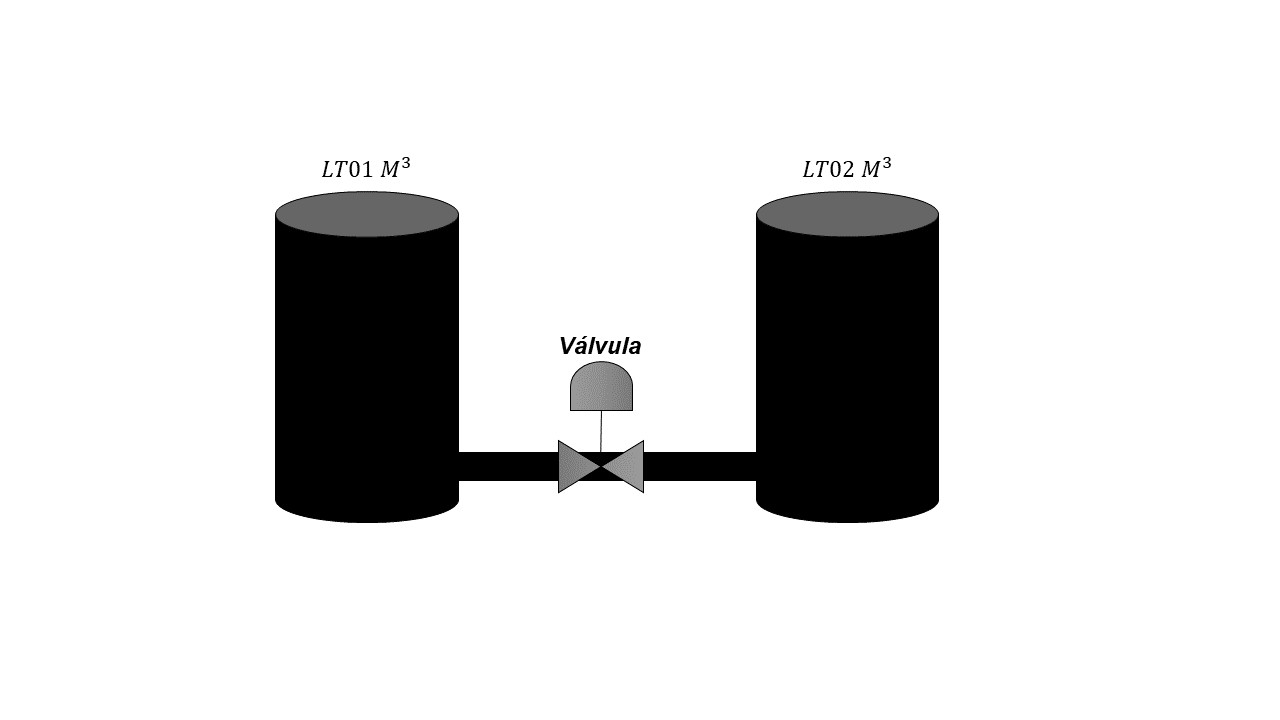
\includegraphics[width=1\linewidth]{Resultados/Figuras/esquema}
	Fonte: Elaboração própria 
\end{figure}

Na Figura \ref{fig:esquema} um esquema pratico para evitar a falta de água e o consumo em horários de pico. Esse esquema é bem simples de como pode ser melhorado o aproveitado de tempo no período do dia para armazenamento de água.

Na \ref{q3} o tanque tem como máximo nos dados $4,256 m^3$ dano em litros $4256$L para atender essa demanda e manter o tanque quase cheio ou sempre cheio, a Vasão de entrada tem que estar em $[238,302] \ m^3/h$, vasão de gravidade tem que ficar entre $[126,182] m^3/h$, vasão de recalque entre $[110,144] m^3/h$, pressão de sucção entre $[1.92,4.24] mca$ pressão de recalque entre $[21,24] mca$.

Na \ref{q4} o ponto de equilibro para não ser acionado as bomba seria de as vazão FT01 $211 m^3/h$  FT02 $114 m^3/h$ FT03 $100m^3/h$ e o nível do tanque com $3,545 m^3$.

Na \ref{q5:a} o tanque deve estar com o nível de $4,00 m^3$ para que não precise acionar bombas no horário de pico. 

\subsubsection{M\'ultiplas entradas e sa\'ida \'unica (MISO)}

Nessa \ref{etp:2} o modelos que mais foi abordado no decorrer da dissertação é os modelos ARIMA, ou os que derivam desse modelo, e os modelos regressivo fora o LR  tem múltiplas entra e uma saída da variável que é prevista o LT01, as outras variáveis serve de apoio para melhorar os modelos do tipo ARX ou modelos com variáveis exógenas. Os modelos ARIMA sem a variável exógena é apenas um entrada, semelhante com o LR.



\subsubsection{Decomposi\c c\~ao STL}

 \citeonline{Theodosiou20111178} A decomposição sazonal e tendencial utilizando o procedimento de Loess (STL) é utilizada para a decomposição aditiva da série temporal global. O STL realiza a decomposição aditiva dos dados por meio de uma sequência de aplicações do Loess mais suave, que aplica regressões polinomiais ponderadas localmente em cada ponto do conjunto de dados, sendo as variáveis explicativas os valores mais próximos do ponto cuja resposta está sendo estimada. 
 
 \begin{figure}[H]
 	\centering
 	\caption{Decomposição STL aditiva dos dados coletados}
 	\label{fig:stl-aditiva}
 	\includegraphics[width=1\linewidth]{"Resultados/Figuras/STL aditiva"}
 	
 	Fonte: Elaboração própria a partir de dados da SANEPAR (2018 a 2020)
 \end{figure}
 
 
 \begin{figure}[H]
 	\centering
 	\caption{Decomposição STL multiplicativa dos dados coletados}
 	\label{fig:stl}
 	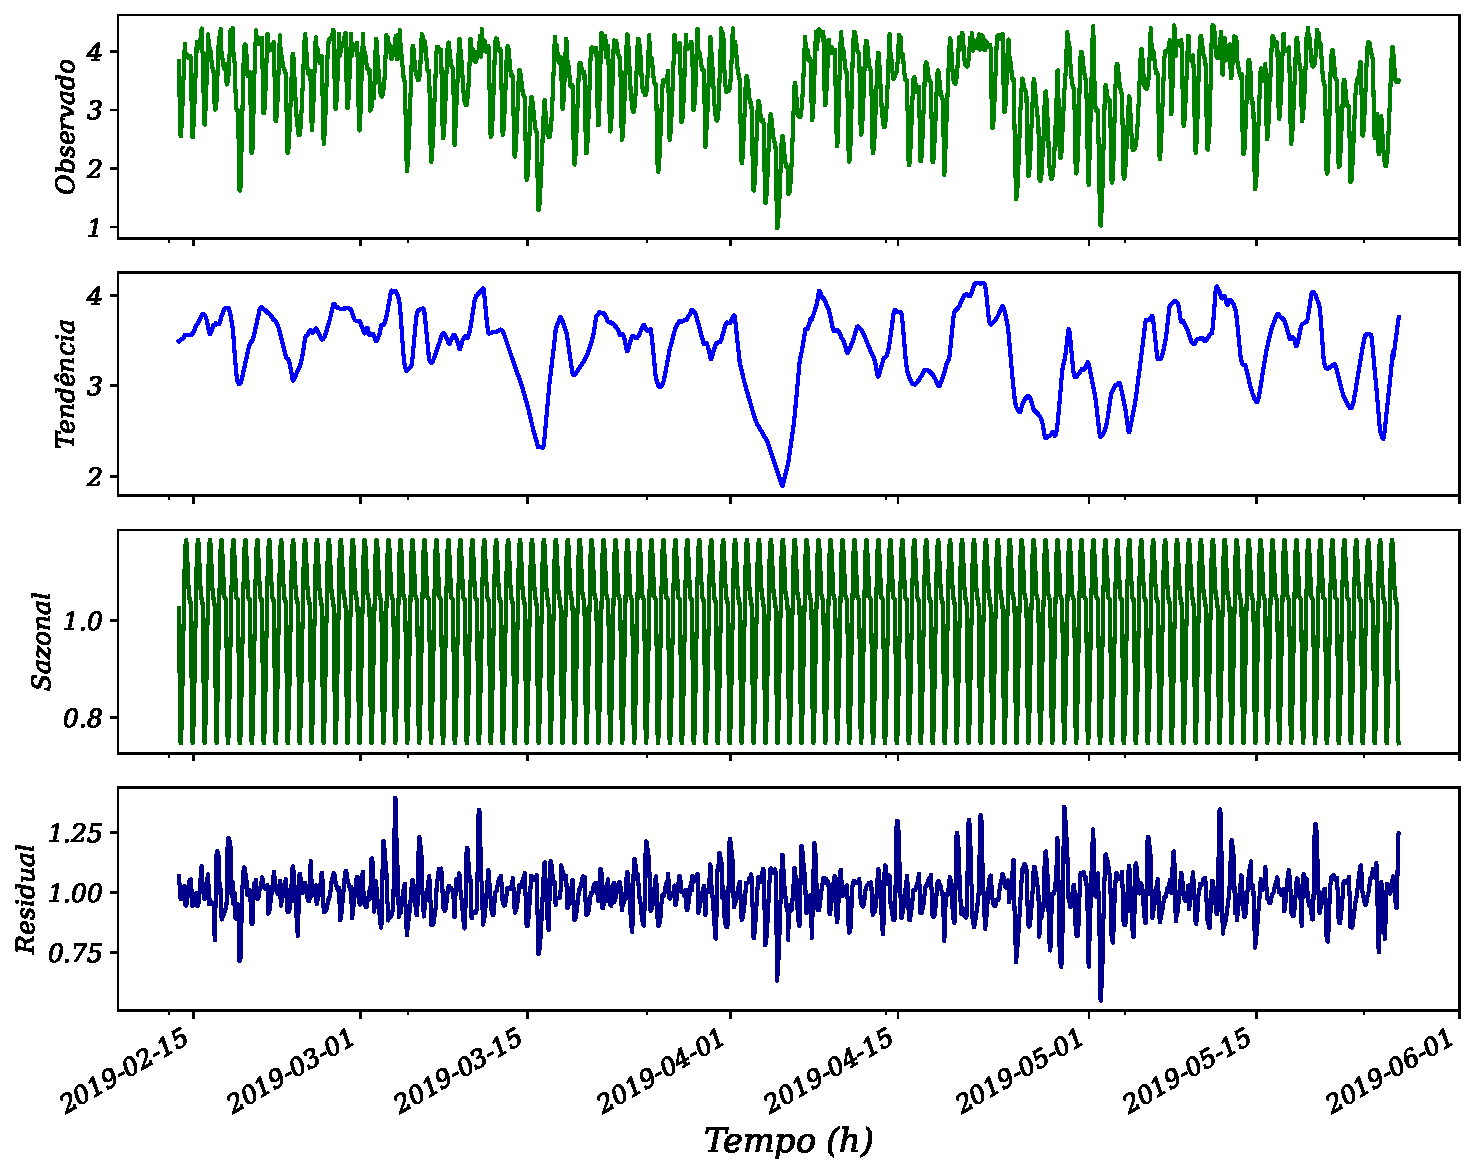
\includegraphics[width=1\linewidth]{Resultados/Figuras/STL}
 	
 	Fonte: Elaboração própria a partir de dados da SANEPAR (2018 a 2020)
 \end{figure}
 
 Na  \ref{q5}\ref{q5:b} pode ser respondida pela Figuras \ref{fig:stl-aditiva} e \ref{fig:stl} como é observado tem tenência, sazonalidade e resido.
 
Na decomposição o objetivo dela é analisar se há tenência, sazonalidade e resido, olhando nas Figuras \ref{fig:stl-aditiva} e \ref{fig:stl}, isso mostra que os dados tem ambas das analise. E com isso perceber que a série é estacionaria, pelo teste a seguir.

Teste de Dickey-Fuller (DF) Aumentado: 
\begin{itemize}
	\item Estatística de teste ADF     $-4.248$
\item $p-valor$                       $0.001$
\item atrasos utilizados         $21.000$
\item  observações              $1074.000$
\item valor crítico $(1\%)           -3.436$
\item valor crítico $(5\%)           -2.864$
\item valor crítico $(10\%)          -2.568$


Fortes provas contra a hipótese nula

Rejeitar a hipótese nula

Os dados não têm raiz unitária e são estacionários, Na \ref{q5}\ref{q5:c} como a serie é estacionaria, para identificar quais os horários de pico entre as 18 até as 21h não é um trabalho fácil, pois se pegar na Figura \ref{fig:hist} pode perceber que no ano de 2020 teve um aumento da demanda nessas horas.

\begin{figure}[H]
	\centering
	\caption{Violino do nível do reservatório}
	\label{fig:hist}
	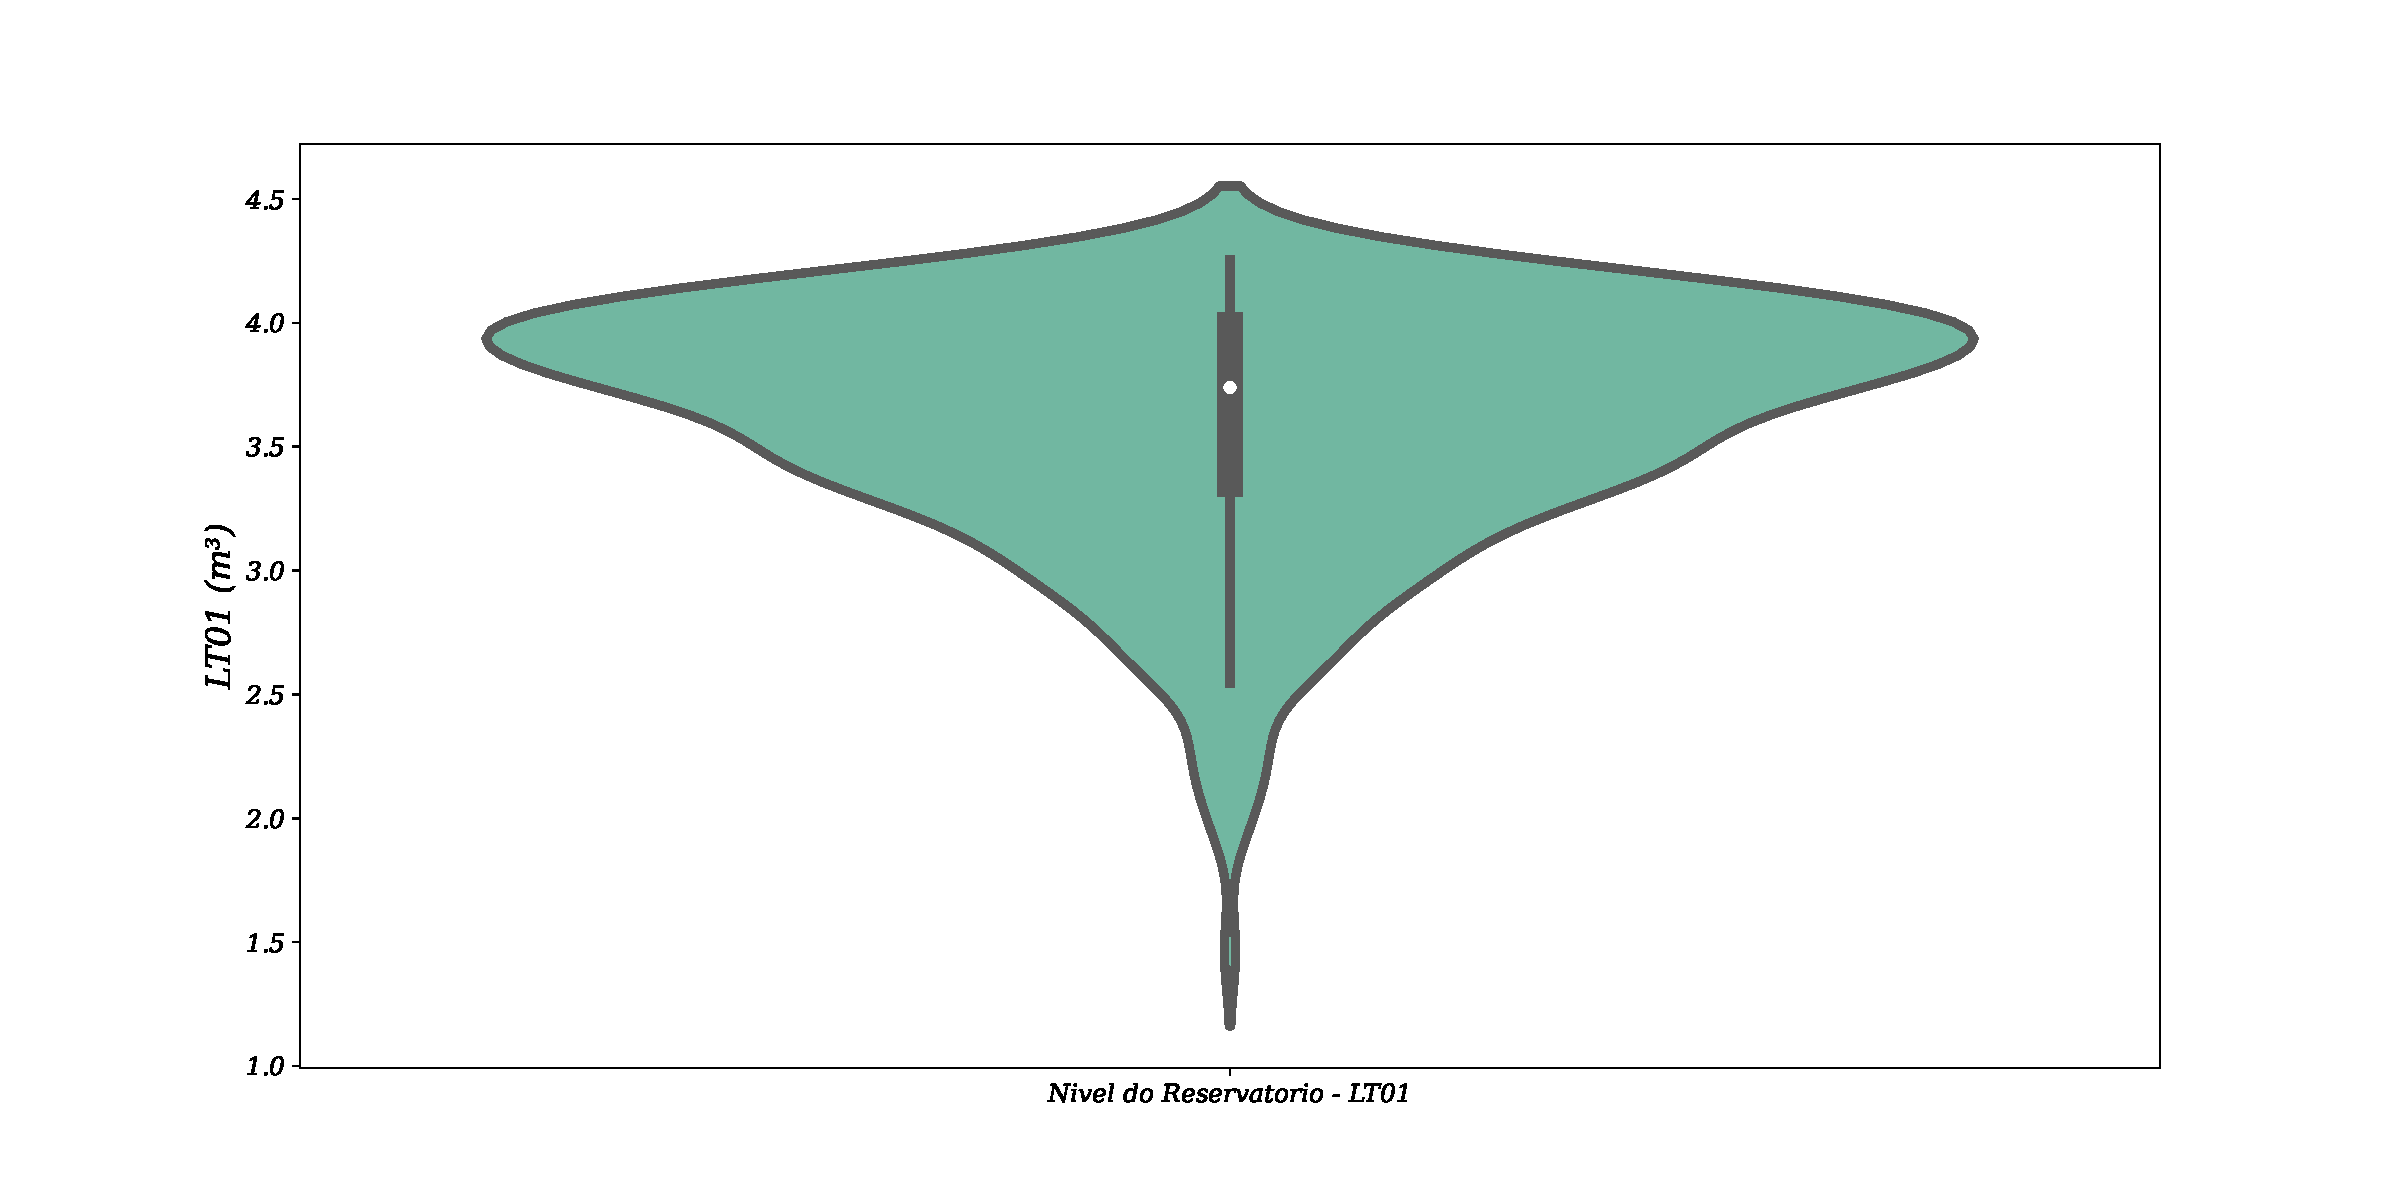
\includegraphics[width=1\linewidth]{Resultados/Figuras/viol}
	
	Fonte: Elaboração própria a partir de dados da SANEPAR (2018 a 2020)
\end{figure}

Então como dito na seção \ref{subsubsec:motivacao} as anomalias de tempo mais ocasionada no ano de 2020 e foi devido a falta de chuva nesse período.

Na \ref{q5}\ref{q5:d} nos horários de picos deve conter no tanque por volta de $[3.545,4.256] m^3$ para que não acione as bombas.



\begin{figure}[H]
	\centering
	\caption{Violino da vazão de recalque}
	\label{fig:ft03}
	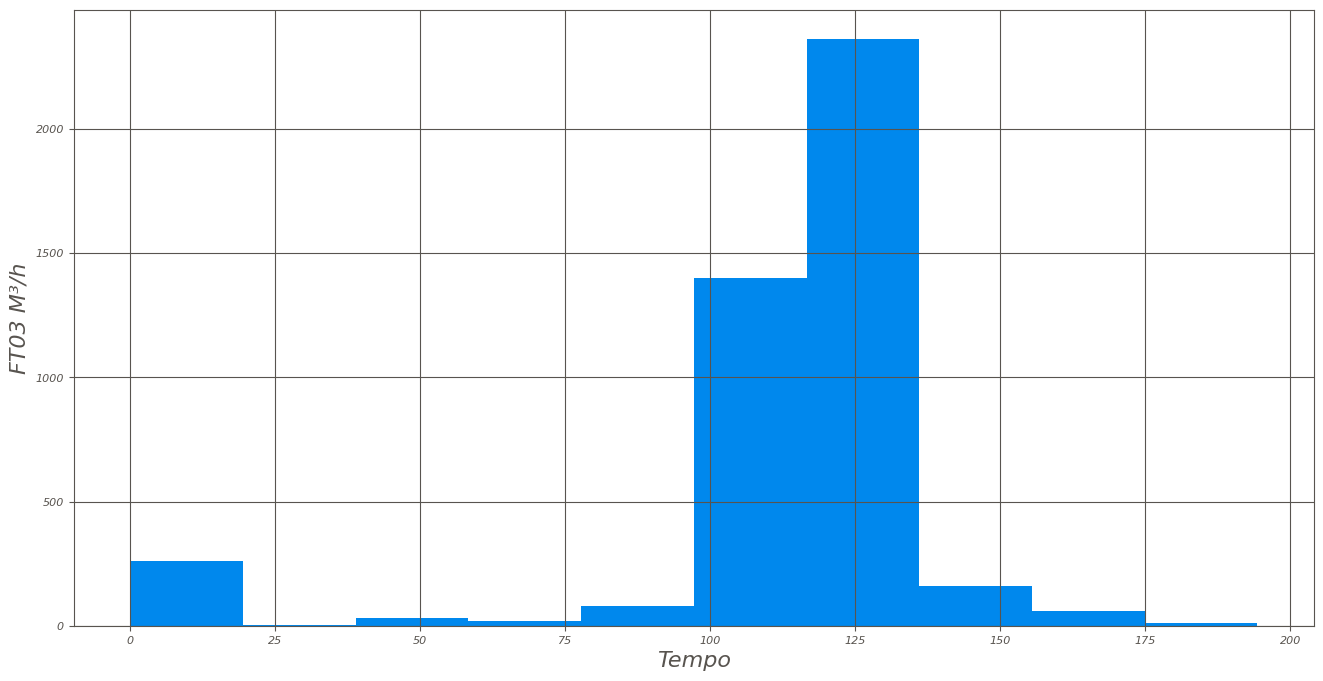
\includegraphics[width=1\linewidth]{Resultados/Figuras/ft03}
	
	Fonte: Elaboração própria a partir de dados da SANEPAR (2018 a 2020)
\end{figure}

Para \ref{q5}\ref{q5:e} é mostrado na Figura \ref{fig:ft03} como pode ser afetado a vazão com o nível do tanque. A vazão de recalque influência mais no nível do tanque que as outras vazão pois injeta água no tanque por meio da bomba de recalque, que fica mais próximo da base do tanque, e as outras vazão por ter alguns valores ausente, não interfere tanto na amostra.

\end{itemize}

Segundo  \citeonline{Reisen2017115} o teste de DF tem como formula a seguinte equações

\begin{eqnarray}
	z_t&=& y_t+\theta \beta_t, \qquad t=1,\ldots, T, \label{eq:df3}\\	
\hat{\rho}_{\mathrm{DF}}-1&=&\frac{\sum_{t=1}^T z_{t-1} \Delta z_t}{\sum_{t=1}^T z_{t-1}^2} \label{eq:regdf}
\end{eqnarray}

De \eqref{eq:regdf} onde $\Delta z_t=z_t-z_{t-1}$. Sob a hipótese nula $\left(H_0\right)$ : `` $\rho=1$'', as estatísticas do teste DF e suas distribuições limitantes são dadas da seguinte forma:


\begin{eqnarray}
	T\left(\hat{\rho}_{\mathrm{DF}}-1\right)=T \frac{\sum_{t=1}^T z_{t-1} \Delta z_t}{\sum_{t=1}^T z_{t-1}^2}
\end{eqnarray}
e


\begin{eqnarray}
	\hat{\tau}_{\mathrm{DF}}&=&\frac{\hat{\rho}_{\mathrm{DF}}-1}{\hat{\sigma}_{\mathrm{DF}}\left(\sum_{t=1}^T z_{t-1}^2\right)^{-1 / 2}} \label{eq:df}
\end{eqnarray}

De \eqref{eq:df} onde $\hat{\sigma}_{\mathrm{DF}}^2=T^{-1} \sum_{t=1}^T\left(\Delta z_t-\left(\hat{\rho}_{\mathrm{DF}}-1\right) z_{t-1}\right)^2 .$



Suponha que $\left(z_t\right)_{1 \leq t \leq T}$ são dadas por \eqref{eq:df3}, então quando $\rho=1$,


\begin{eqnarray}
	T\left(\hat{\rho}_{\mathrm{DF}}-1\right) \stackrel{d}{\longrightarrow} \frac{W(1)^2-1}{2 \int_0^1 W(r)^2 \mathrm{~d} r}-\left(\frac{\theta}{\sigma}\right)^2 \frac{\pi}{\int_0^1 W(r)^2 \mathrm{~d} r}, \text { como } T \rightarrow \infty \\
	\hat{\tau}_{\mathrm{DF}} \stackrel{d}{\longrightarrow}\left[1+2(\theta / \sigma)^2 \pi\right]^{-1 / 2}\left\{\frac{W(1)^2-1}{2\left(\int_0^1 W(r)^2 \mathrm{~d} r\right)^{1 / 2}}-\frac{(\theta / \sigma)^2 \pi}{\left(\int_0^1 W(r)^2 \mathrm{~d} r\right)^{1 / 2}}\right\} \\
	\quad \operatorname{como} T \rightarrow \infty\label{eq:df2}
\end{eqnarray}


De \eqref{eq:df2} onde $\stackrel{d}{\longrightarrow}$ denota a convergência na distribuição e onde $\{W(r), r \in[0,1]\}$ denota o movimento browniano padrão.

Esse teste na literatura é chamado de teste ACF para testar se a série é o não estacionária, basicamente se a série tiver um valor de raiz unitária é uma série não estacionária, do contrario como acontece com os dados coletados se torna uma série estacionária.


\begin{figure}[H]
	\centering
		\caption{Autocorrelação e Autocorrelação parcial}
	\label{fig:acf}
	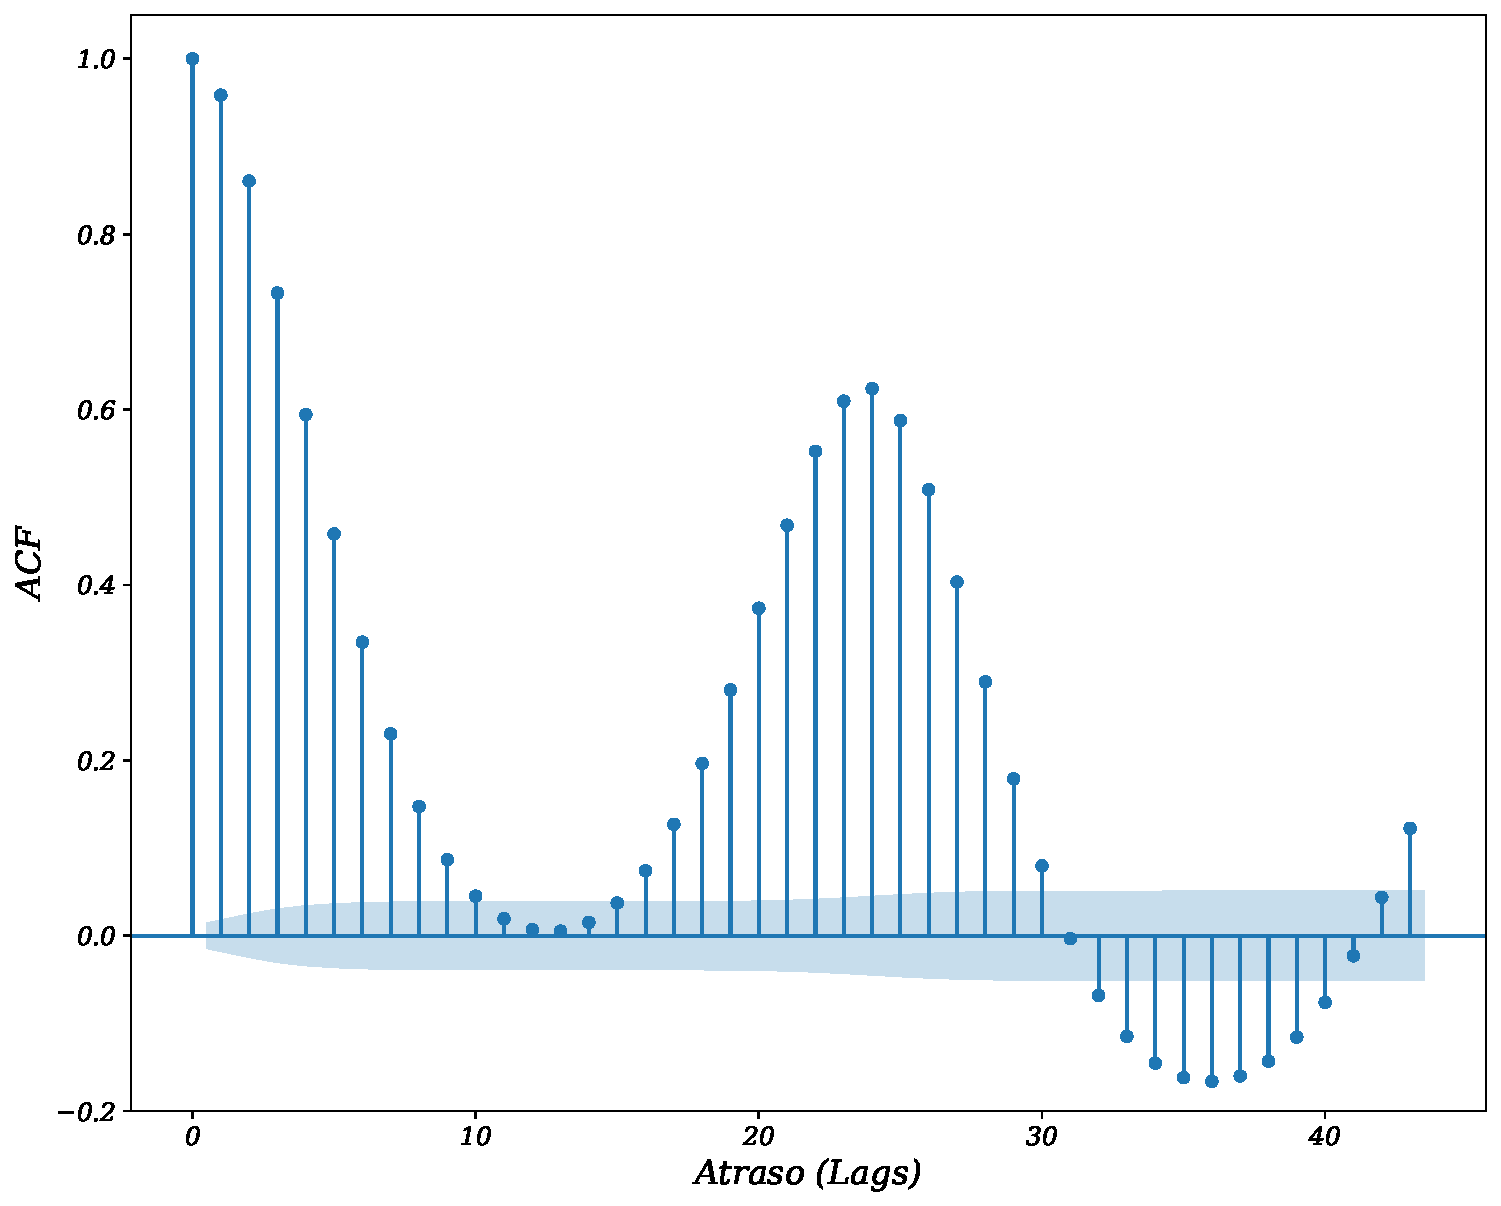
\includegraphics[width=1.1\linewidth]{Resultados/Figuras/acf} 
	
\end{figure}	
\begin{figure}[H]
	\centering
		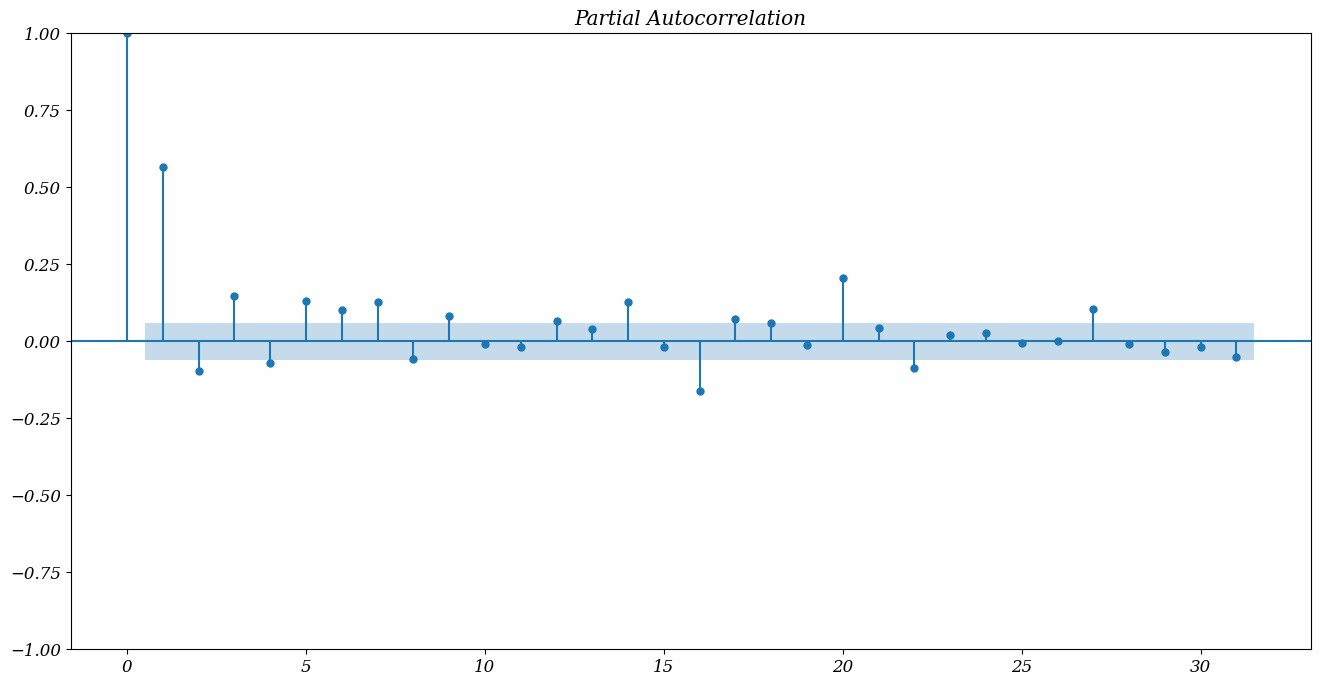
\includegraphics[width=1.1\linewidth]{Resultados/Figuras/pacf}

	Fonte: Elaboração própria a partir de dados da SANEPAR (2018 a 2020)
\end{figure}


Na Figura \ref{fig:acf} tem a diferença entre a autocorrelação e a autocorrelação parcial (PACF) é quase um detalhe em uma ACF temos a correlação direta e indireta e em uma PACF apenas a correlação direta. 

O intervalo de confiança por padrão é 95\%, mostrado como essa marca azul. Observações que estão para fora da marca são consideradas estatisticamente correlacionadas.

As correlação da Figura \ref{fig:acf} é a explicação do teste de DF, entendo isso pode ser visto o próximo passo que é  a análise do ruído branco em meados a gráfico, Uma série ruído branco é uma série na qual a média 0, a variância é constante ao longo da série toda e não há correlação entre os períodos de tempo. O valores de uma série ruídos brancos são totalmente aleatórios, ou seja, essa é um tipo de série que não é previsível.

\begin{figure}[H]
	\centering
	\caption{Ruído branco}
	\label{fig:ruido-branco}
	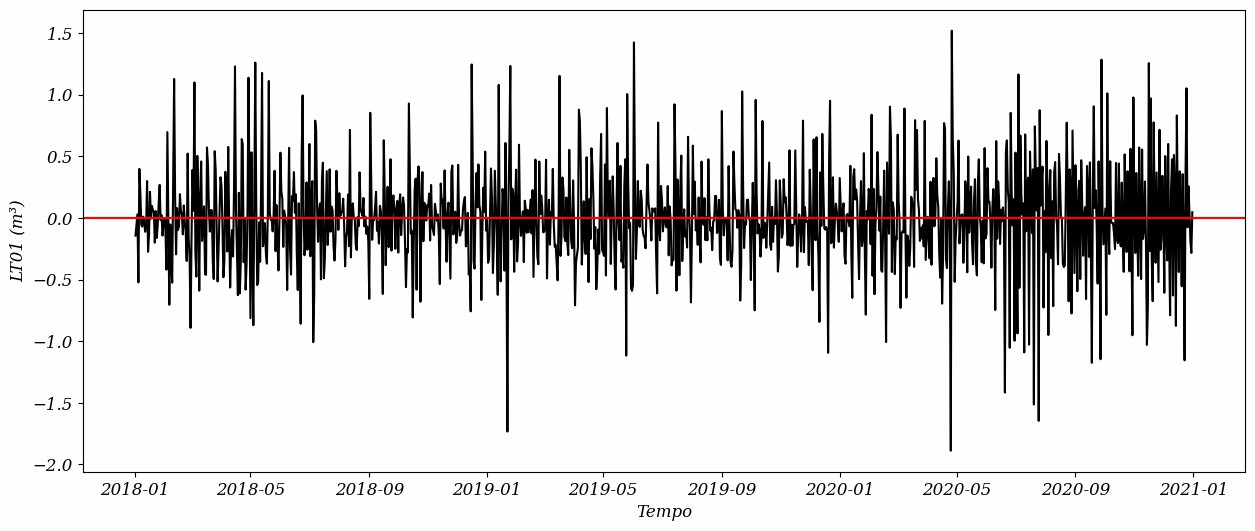
\includegraphics[width=1\linewidth]{Resultados/Figuras/ruido-branco}
	
	Fonte: Elaboração própria a partir de dados da SANEPAR (2018 a 2020)
\end{figure}

Da Figura \ref{fig:ruido-branco} uma série temporal pode ser ruído branco.
Uma série temporal é ruído branco se as variáveis são independentes e distribuídas de forma idêntica com uma média de zero.
Isso significa que todas as variáveis têm a mesma variância ($\sigma^2$) e cada valor tem uma correlação zero com todos os outros valores da série.
Mais para frente vamos mostrar o comprimento de zeros na variável prevista. Com isso encerra a \ref{etp:3}.

\subsubsection{Separa\c c\~ao dos Dados}

Na \ref{etp:4} tem um esquema de como foi dividido os dados em treino, teste e validação, essa pratica é comum para os profissionais de aprendizado de máquina, pois assim como não é passível processar os dados todos de uma vez, se você manosear dados em uma escala menor até pode ser realizado, mas tudo depende da máquina que esta sendo realizado o processamento dos dados, cada modelo em particular utiliza um certo acervo do seu computador para processar, se por exemplo você tiver trabalhando com um modelo de aprendizado profundo que é mais comum em processamento de imagem, a Nvidia tem sempre inovado com as suas GPUs e trazendo mais poder para processamento, com o recente lançamento da placa de vídeo $3090$ um sonho de consumo para games e os profissionais de aprendizado de maquina e profundo.

Em fim se o computador que foi realizado os processamento fosse um computador não tão bom, ainda poderia está sendo pensando que estaria em processamento, sem as inovação que foi estabelecida aos anos, o computador que foi realizado os cálculos dos modelos foi em partes um computador de processador $i5-3300$ e um notebook com $i7-5500$ ambos com 4 threads e o notebook com apenas 2 núcleos o $i5$ contem 4 núcleos. Cada um tem suas especificações de ser o melhor em algum certo ponto, mas sabendo que não é preciso de um de ultima geração para fazer tais processamento. E sim força de vontade para entende e aplicar em cada um.

A divisão mais básica que tem na literatura foi realizada aqui na separação dos dados, $70\%$ para treino e os $30\%$ restante para teste, dos $70\%$ tem mais uma divisão pegando $80\%$ dos $70\%$ para treino novamente e os $20\%$ para validação dos dados, tendo essa fórmula aplica na linguagem de programação para que não precisa ser contado todas as vezes que for mudado o modelo.

\subsubsection{Estrategia de Previs\~ao}\label{subsubsec:est}

Na \ref{etp:5} é abordado a forma que foi previsto os dados, em uma janela de horizonte de previsão bem maior do que o normal na literatura da estrategia de recursiva, sendo 1, 7, 14 e 30 dias previsto, essa estrategia para comparação dos modelos regressivo e modelos ARIMA, é bem vantajoso, pois cada modelo tem suas especificidade para prever em momentos com janela de tempo menor e com uma janela de muitos dias. Assim como explicado na seção \ref{subsubsec:modelos} se for previsão curta, alguns vai se sobre por em meio à outros modelos que foi feito aqui.

\subsubsection{Horizonte}

Na \ref{etp:6} é feito o horizonte de previsão, como dito na seção \ref{subsubsec:est} esse horizonte foi customizado baseado do método recursivo de prever as series temporais e a previsão do nível do tanque LT01. Os passos para prever a frente foi de 1, 7, 14 e 30 dias, já foi realizado uma estrategia com uma janela menor, mas para comparação dos modelos essa janela foi mais adequada.

\subsubsection{Modelos de previs\~ao e m\'etricas de desempenho}\label{subsubsec:modelos}

Da \ref{etp:7} as métricas utilizada aqui foi vista na seção \ref{subsec:metrica} foi utilizado aqui três das métricas mais usada na literaturar para previsão de tempo e comparação de modelos ARIMA e os modelos regressores.

    Em comparação com os modelos feito, pode ser visto que o modelo LR em um passo a frente tem tanto na modelagem de 24 horas quanto no pico de horas entre as 18 e 21 horas, foi o modelo que mais se saiu bem na previsão, logo em sequência os modelos MA, AR, SARIMA, ARIMA, SARIMAX, ARIMAX, ARX, LGBMRegressor, XGBRegressor e Random Forest Regressor, para curto prazo esses modelos estão em ordem de melhor para pior.
    
    Já em grande espaço de tempo como foi feito de 30 dias os modelos ARMA, AR, MA, ARIMA, ARIMAX, ARX, SARIMAX, SARIMA, XGBRegressor, Random Forest Regressor, LGBMRregressor e LR, seguindo a mesma lógica do melhor para o pior. Mas se olhar graficamente nos modelos que foi feito, os modelos com variáveis exógenas aparenta prever melhor do que os outros modelos, só analisando os dados nos apêndice tanto quando as Figuras de \ref{fig:1-AR-ARX-MA24} a \ref{fig:60-LR-XGB-LGBM-RF24} quanto as Tabalas \ref{tb:1-24trn} a \ref{tb:60-24cm}   
    
    \subsubsection{Teste de Signific\^ancia}
    
    Na \ref{etp:9} os teste escolhido foi de \textit{Friedman e Nemenjy} no teste de Nemenyi, precisamos obter a diferença entre os rankings médios (linha média da tabela de classificação) entre todos os classificadores (comparando pares de classificadores). Se essa diferença for maior ou igual a um CD (distância crítica), podemos dizer que esses dois classificadores são significativamente diferentes um do outro. O CD é calculado como:
    
    \begin{eqnarray}
    	C D&=&q_\alpha \sqrt{\frac{k(k+1)}{6 N}}\label{eq:neme}
    \end{eqnarray}

De \eqref{eq:neme} o termo $q_\alpha$ é obtido de ($\alpha=0,05$):

\begin{table}[H]
	\centering
	\caption{Teste Nemenyi}
	\begin{tabular}{@{}clllllllll@{}}
		\toprule
		\multicolumn{1}{l}{\textbf{Nemenyi}} & \multicolumn{1}{c}{\textbf{0}} & \multicolumn{1}{c}{\textbf{1}} & \multicolumn{1}{c}{\textbf{2}} & \multicolumn{1}{c}{\textbf{3}} & \multicolumn{1}{c}{\textbf{4}} & \multicolumn{1}{c}{\textbf{5}} & \multicolumn{1}{c}{\textbf{6}} & \multicolumn{1}{c}{\textbf{7}} & \multicolumn{1}{c}{\textbf{8}} \\ \midrule
		\textbf{0}                           & 1,000                          & 0,001                          & 0,001                          & 0,001                          & 0,001                          & 0,001                          & 0,001                          & 0,001                          & 0,001                          \\
		\textbf{1}                           & 0,001                          & 1,000                          & 0,001                          & 0,001                          & 0,001                          & 0,001                          & 0,001                          & 0,001                          & 0,157                          \\
		\textbf{2}                           & 0,001                          & 0,001                          & 1,000                          & 0,847                          & 0,001                          & 0,001                          & 0,001                          & 0,001                          & 0,001                          \\
		\textbf{3}                           & 0,001                          & 0,001                          & 0,847                          & 1,000                          & 0,001                          & 0,001                          & 0,001                          & 0,001                          & 0,001                          \\
		\textbf{4}                           & 0,001                          & 0,001                          & 0,001                          & 0,001                          & 1,000                          & 0,001                          & 0,001                          & 0,001                          & 0,001                          \\
		\textbf{5}                           & 0,001                          & 0,001                          & 0,001                          & 0,001                          & 0,001                          & 1,000                          & 0,001                          & 0,001                          & 0,001                          \\
		\textbf{6}                           & 0,001                          & 0,001                          & 0,001                          & 0,001                          & 0,001                          & 0,001                          & 1,000                          & 0,001                          & 0,001                          \\
		\textbf{7}                           & 0,001                          & 0,001                          & 0,001                          & 0,001                          & 0,001                          & 0,001                          & 0,001                          & 1,000                          & 0,001                          \\
		\textbf{8}                           & 0,001                          & 0,157                          & 0,001                          & 0,001                          & 0,001                          & 0,001                          & 0,001                          & 0,001                          & 1,000                          \\ \bottomrule
	\end{tabular}

Fonte: Elaboração própria a partir de dados da SANEPAR (2018 a 2020)
\end{table}

O teste de Nemenyi (Nemenyi, 1963) é um teste \textit{post-hoc}, ou seja, é um teste de comparação múltipla que é usado após a aplicação de teste não paramétricos com três ou mais fatores.
    
Para calcular a estatística de teste $F_r$ de Friedman cria-se inicialmente uma tabela com os dados, colocando-se em cada linha uma amostra e cada coluna correspondendo a uma condição de teste. A seguir, as amostras ao longo das condições são ordenadas, da melhor situação para a pior. Se não houver empates, usa-se a equação \eqref{eq:fr} para determinar a estatística de teste $F_r$:

\begin{eqnarray}
	F_r&=&\left[\frac{12}{n k(k+1)} \sum_{i=1}^k R_i{ }^2\right]-3 n(k+1)\label{eq:fr}
\end{eqnarray}
  
  Na equação \eqref{eq:fr} $n$ é o número de linhas (ou amostras), $k$ é o número de colunas (ou condições) e $R_i$ é a soma dos postos da coluna (ou condição) $i$.   
 Seguindo a equação \eqref{eq:fr} têm o seguinte resultado nos dados da pesquisa.
 
 $statistic=8015.611,\ \ pvalue=0.0$ com o números de 26306 linhas x 9 colunas.
 
 \subsubsection{Compara\c c\~ao dos modelos}
 Nos modelos coletados com várias métodos de prever, com isso para ver melhor como cada modelo se comporta foi realizado a comparação dos modelos em base com o gráfico violino, assim observa quais os melhores entre os modelos coltado.
 
 \begin{figure}[H]
 	\centering
 	\caption{Comparação de modelos ARIMAS}
 	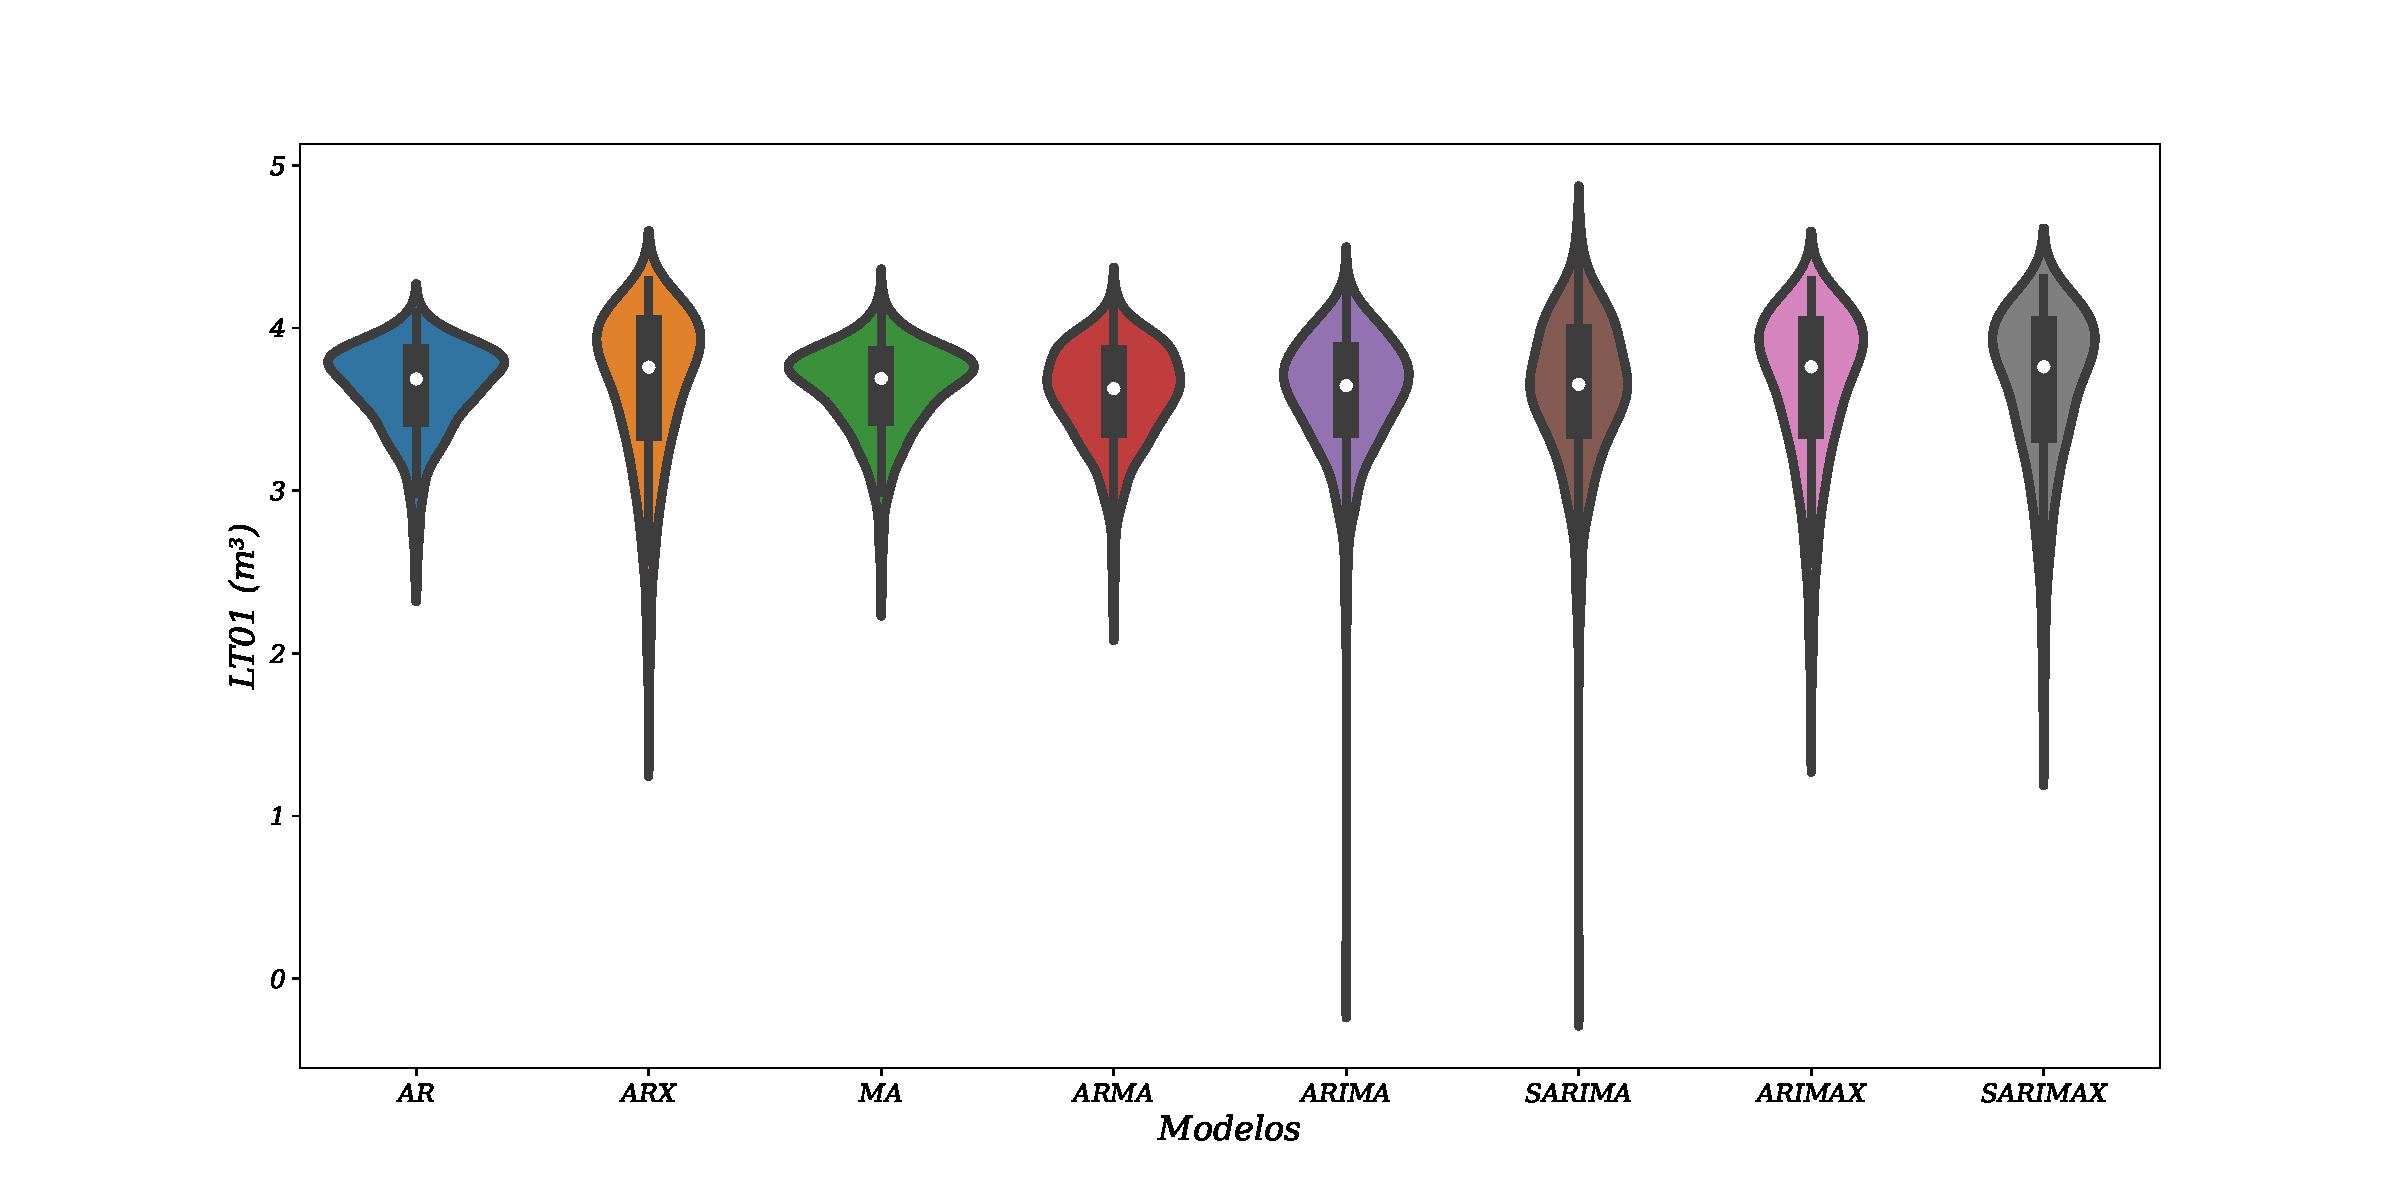
\includegraphics[width=0.9\linewidth]{Resultados/Figuras/modelos-arima}
 	
 	\label{fig:modelos-arima}
 	
 	Fonte: Elaboração própria a partir de dados da SANEPAR (2018 a 2020)
 \end{figure}
 
 
 \begin{figure}[H]
 	\centering
 	\caption{Comparação de modelos de regressão }
 	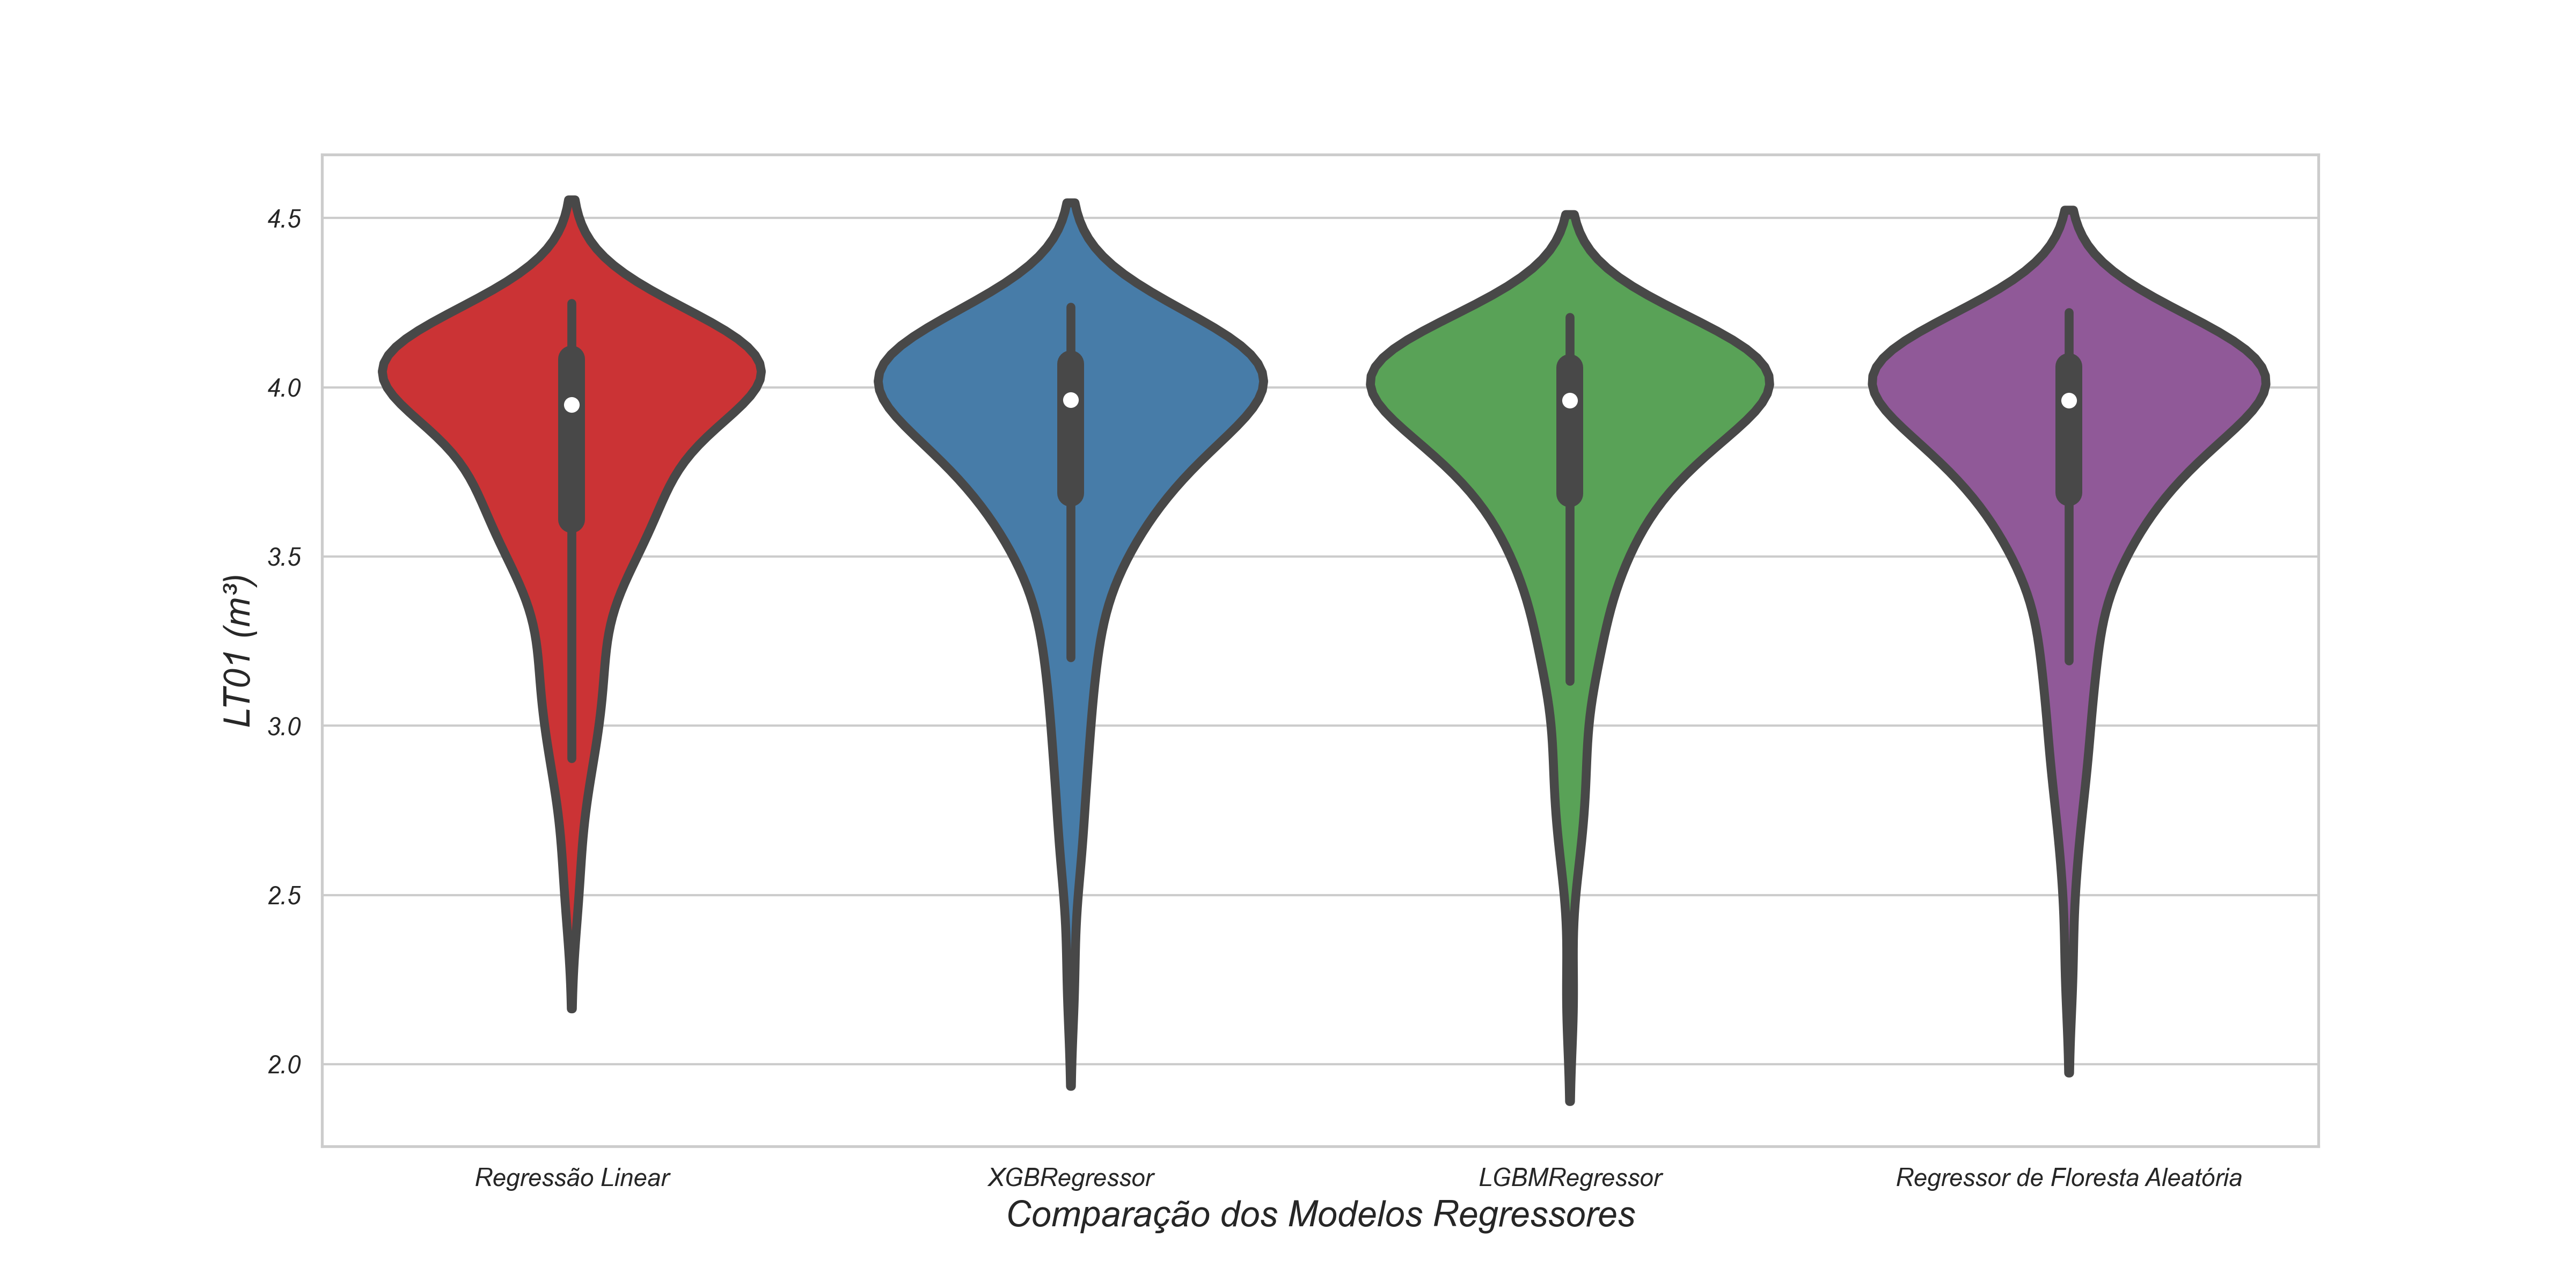
\includegraphics[width=0.9\linewidth]{Resultados/Figuras/violin-LR-XGB-LGBM-RF}
 	
 	\label{fig:violin-lr-xgb-lgbm-rf}
 	
 	Fonte: Elaboração própria a partir de dados da SANEPAR (2018 a 2020)
 \end{figure}


Em comparação com os modelos apresentado nas Figuras \ref{fig:modelos-arima} e \ref{fig:violin-lr-xgb-lgbm-rf} os modelos que pode ser observado que são os melhores levando em conta a modelagem dos dados, nos modelos ARIMA os melhores são AR, ARX, MA, ARMA, ARIMAX e SARIMAX, devido ao \textit{outliers} e ao limite inferior de alguns modelos, olhando para os modelos de gradiente e regressão, pode se notar que eles ficaram similar, devido a técnicas de otimização matemática Grid Search (do inglês pesquisa grande) e Randomized Search (do inglês pesquisa aleatória), que possibilitou a melhora do método utilizado. Em um horizonte de previsão pequeno o LR prevê melhor que os outros modelos, mas em um horizonte de previsão maior os modelos XGBoost e Light GBM estão prevendo com melhor rigor. O floresta aleatória está prevê com rigor também só vindo atrás do XGBoost em previsão de longo prazo.

O método de Ljung box é um método que pode ser estimados a longo prazo os modelos ARIMAS se a longo prazo eles ainda vão prever com eficiência nos dados, a longo prazo os modelos que melhor prevê são os modelos ARX, ARIMAX e SARIMAX com as variáveis exógena para modelos não linear ele consegue se manter por mais tempo prevendo do que os outros modelos ARIMA.  
 
  
    

    


%% CONCLUSÕES
\section{Conclus\~oes} \label{sec:conclusoes}

Nessa dissertação teve como objetivo, conduziu-se um estudo abrangente sobre a previsão da demanda d'água por meio da análise de séries temporais. Através da análise exploratória dos dados e da aplicação da decomposição STL, identificaram-se padrões sazonais e tendências na demanda d'água. Durante o estudo, os modelos DT e Prophet foram empregados para validar o estudo de caso da SANEPAR.

Os objetivos específicos do estudo foram alcançados, contribuindo significativamente para a compreensão e aplicação de modelos de previsão de séries temporais na gestão da demanda d'água.

Aplicar diferentes modelos de previsão de séries temporais utilizando dados provenientes do Bairro Alto em Curitiba, fornecidos pela SANEPAR.
A aplicação de diferentes modelos de previsão, utilizando dados específicos do Bairro Alto em Curitiba fornecidos pela SANEPAR, permitiu avaliar sua precisão, eficiência e capacidade de previsão em conjuntos de dados específicos, utilizando medidas de desempenho para análise.

Avaliar a precisão, eficiência e capacidade de previsão desses modelos em conjuntos de dados específicos, utilizando métricas para análise de desempenho.

Explorar estratégias de otimização baseadas em otimização Bayesiana, empregando o algoritmo TPE para ajustar os hiperparâmetros dos modelos de previsão de séries temporais.
A exploração de estratégias de otimização baseadas em otimização Bayesiana, empregando o algoritmo TPE para ajustar os hiperparâmetros dos modelos, resultou na identificação de combinações eficazes de modelos de previsão de séries temporais em conjunto com a configuração otimizada.

Identificar combinações eficazes de modelos de previsão de séries temporais em conjunto com a configuração otimizada. 

Avaliar o impacto das variáveis exógenas na melhoria da precisão dos modelos de previsão de séries temporais.

Os resultados obtidos demonstram que a abordagem de séries temporais é uma ferramenta eficaz para prever a demanda futura d'água, destacando a importância de considerar as flutuações sazonais e as diferentes partes do dia ao determinar a vazão e o volume mínimo de reserva no reservatório.

Esses objetivos específicos não apenas cumpriram sua função original, mas também forneceram informações para a otimização do planejamento e operação de sistemas de abastecimento d'água, promovendo a resiliência diante de variações sazonais e eventos imprevistos. Essa pesquisa pode ser aplicado na prática, auxiliando gestores e tomadores de decisão na implementação de estratégias mais eficientes para garantir o abastecimento d'água de forma sustentável e resiliente.

O estudo de casos separados em dois tipos de análise de padrões e consumo e o outro estratégia de economia de energia tem como foco melhorar o consumo d'água em horários de pico e otimizar a demanda d'água para que não seja afetada novamente no futuro e falte água novamente. Usando os modelos, consegue-se responder a três questões de pesquisa feitas nessa dissertação. A primeira foi entender os dados se existe tendência, padrão e sazonalidade, para o tratamento que foi realizado, o qual foi muito bom para entender os dados.

A segunda questão já teve a ver com o impacto no acionamento das bombas em horário de pico, confirmando assim que no horário de pico o gasto de energia e a demanda d'água são maiores, mas com uma pequena estratégia pode-se contornar isso facilmente. A terceira questão é quanto deve ser armazenado previamente no reservatório LT01 para que não seja necessário ter esse gasto de energia, $4.445$ litros é o suficiente para que o reservatório passe o horário de pico com o menor gasto energético.

 


\subsection{Propostas Futuras}

Apesar dos resultados promissores evidenciados por esta pesquisa, é essencial que se reconheçam suas limitações e que se instigue a exploração de novos horizontes em pesquisas subsequentes. Uma análise mais profunda e abrangente pode ser realizada, investigando modelos de redes neurais mais avançados. Além disso, a implementação de técnicas de otimização matemática mais refinadas, como o uso do método \textit{Covariance Matrix Adaptation Evolution Strategy} (CMAES), pode ser considerada. Seria prudente incluir cuidadosamente variáveis exógenas em todos os modelos pertinentes, como o uso de variáveis climáticas e dados de precipitação do tempo.
Implementa modelos que utilizam sistemas \textit{fuzzy} para aprimorar a previsão do tanque. Usa essa previsão juntamente com modelos existentes na literatura, como a otimização \textit{Bayesian Optimization Algorithm} (BOA), que não foi abordada neste contexto.





%-----------------------------------------------------------------
%% ELEMENTOS POS-TEXTUAIS

%% BIBLIOGRAFIA
\addcontentsline{toc}{section}{Refer\^encias} %% ADICIONA REFERÊNCIAS NO SUMÁRIO
	\bibliography{Bibliografia/Dissert2}
	

%% APÊNDICES
\appendix

%% TABELAS


%\begin{landscape}


\section{Ap\^endice - Compara\c c\~ao dos modelos de previs\~ao de series temporais m\'edia de 24h}\label{sec:comtb24}

Nas tabelas do apêndice todos os valores estão multiplicado por 100 com isso sendo os valores uma porcentagem de erro.

$(p = 7,d = 1,q = 7) (P = 2,D = 1,Q = 1)_{M = 12}$ média 24h
	\begin{table}[H]
	\centering
	\caption{Comparação dos modelos 1 dia a frente 24h \textbf{Treino} }\label{tb:1-24trn}
	\begin{tabular}{@{}clll@{}}
		\toprule
		\multirow{2}{*}{\textbf{Modelos}} & \multicolumn{3}{c}{\textbf{Erros}}                                                                       \\ \cmidrule(l){2-4} 
		& \multicolumn{1}{c}{\textbf{MAPE}} & \multicolumn{1}{c}{\textbf{MAE}} & \multicolumn{1}{c}{\textbf{RMSE}} \\ \hline
\textbf{AR}                       & 10,096                            & 31,825                           & 41,271                            \\
\textbf{ARX}                      & 13,785                            & 44,369                           & 57,035                            \\
\textbf{MA}                       & 10,182                            & 31,979                           & 41,791                            \\
\textbf{ARMA}                     & 10,529                            & 33,288                           & 43,011                            \\
\textbf{ARIMA}                    & 10,525                            & 33,580                           & 43,084                            \\
\textbf{SARIMA}                   & 11,660                            & 37,174                           & 50,113                            \\
\textbf{ARIMAX}                   & 13,778                            & 44,296                           & 57,081                            \\
\textbf{SARIMAX}                  & 13,765                            & 44,291                           & 56,655                            \\
\textbf{Linear Regression}        & 2,162                             & 9,798                            & 11,454                            \\
\textbf{Random Forest Regressor}  & 19,142                            & 60,207                           & 67,351                            \\
\textbf{XGBRegressor}             & 17,901                            & 56,218                           & 64,009                            \\
\textbf{LGBMRegressor}            & 19,309                            & 60,878                           & 68,006                            \\ \bottomrule
	\end{tabular}

Fonte: Elaboração própria a partir de dados da SANEPAR (2018 a 2020)
\end{table}

\begin{table}[H]
	\centering
	\caption{Comparação dos modelos 1 dia a frente 24h \textbf{Validação} }\label{tb:1-24vld}
	\begin{tabular}{@{}clll@{}}
		\toprule
		\multirow{2}{*}{\textbf{Modelos}} & \multicolumn{3}{c}{\textbf{Erros}}                                                                       \\ \cmidrule(l){2-4} 
		& \multicolumn{1}{c}{\textbf{MAPE}} & \multicolumn{1}{c}{\textbf{MAE}} & \multicolumn{1}{c}{\textbf{RMSE}} \\ \hline
\textbf{AR}                       & 9,869                             & 34,944                           & 43,912                            \\
\textbf{ARX}                      & 12,850                            & 45,890                           & 55,194                            \\
\textbf{MA}                       & 9,733                             & 34,586                           & 43,500                            \\
\textbf{ARMA}                     & 10,439                            & 37,222                           & 46,820                            \\
\textbf{ARIMA}                    & 10,320                            & 37,395                           & 45,758                            \\
\textbf{SARIMA}                   & 12,216                            & 44,456                           & 62,635                            \\
\textbf{ARIMAX}                   & 12,871                            & 45,948                           & 54,964                            \\
\textbf{SARIMAX}                  & 13,049                            & 46,682                           & 57,124                            \\
\textbf{Linear Regression}        & 2,661                             & 13,071                           & 14,533                            \\
\textbf{Random Forest Regressor}  & 12,656                            & 43,646                           & 53,263                            \\
\textbf{XGBRegressor}             & 11,705                            & 40,399                           & 49,187                            \\
\textbf{LGBMRegressor}            & 12,782                            & 44,104                           & 53,659                            \\ \bottomrule
	\end{tabular}

Fonte: Elaboração própria a partir de dados da SANEPAR (2018 a 2020)
\end{table}

\begin{table}[H]
	\centering
	\caption{Comparação dos modelos 1 dia a frente 24h \textbf{Teste} }\label{tb:1-24tst}
	\begin{tabular}{@{}clll@{}}
		\toprule
		\multirow{2}{*}{\textbf{Modelos}} & \multicolumn{3}{c}{\textbf{Erros}}                                                                       \\ \cmidrule(l){2-4} 
		& \multicolumn{1}{c}{\textbf{MAPE}} & \multicolumn{1}{c}{\textbf{MAE}} & \multicolumn{1}{c}{\textbf{RMSE}} \\ \hline
\textbf{AR}                       & 10,849                            & 38,196                           & 48,482                            \\
\textbf{ARX}                      & 12,476                            & 44,531                           & 58,255                            \\
\textbf{MA}                       & 11,800                            & 41,355                           & 51,227                            \\
\textbf{ARMA}                     & 11,749                            & 41,936                           & 51,845                            \\
\textbf{ARIMA}                    & 11,740                            & 41,999                           & 51,233                            \\
\textbf{SARIMA}                   & 12,368                            & 44,720                           & 54,802                            \\
\textbf{ARIMAX}                   & 12,488                            & 44,554                           & 58,346                            \\
\textbf{SARIMAX}                  & 12,630                            & 45,116                           & 59,116                            \\
\textbf{Linear Regression}        & 2,821                             & 13,896                           & 15,006                            \\
\textbf{Random Forest Regressor}  & 10,481                            & 35,920                           & 45,772                            \\
\textbf{XGBRegressor}             & 9,738                             & 33,332                           & 42,630                            \\
\textbf{LGBMRegressor}            & 11,297                            & 38,952                           & 49,002                            \\ \bottomrule
	\end{tabular}

Fonte: Elaboração própria a partir de dados da SANEPAR (2018 a 2020)
\end{table}

\begin{table}[H]
	\centering
	\caption{Comparação dos modelos 1 dia a frente 24h \textbf{Completo} }\label{tb:1-24cm}
	\begin{tabular}{@{}clll@{}}
		\toprule
		\multirow{2}{*}{\textbf{Modelos}} & \multicolumn{3}{c}{\textbf{Erros}}                                                                       \\ \cmidrule(l){2-4} 
		& \multicolumn{1}{c}{\textbf{MAPE}} & \multicolumn{1}{c}{\textbf{MAE}} & \multicolumn{1}{c}{\textbf{RMSE}} \\ \hline
\textbf{AR}                       & 9,750                             & 32,207                           & 17,093                            \\
\textbf{ARX}                      & 13,396                            & 45,125                           & 32,940                            \\
\textbf{MA}                       & 12,297                            & 40,335                           & 50,963                            \\
\textbf{ARMA}                     & 9,860                             & 32,774                           & 42,069                            \\
\textbf{ARIMA}                    & 10,080                            & 33,536                           & 42,805                            \\
\textbf{SARIMA}                   & 11,803                            & 40,028                           & 50,689                            \\
\textbf{ARIMAX}                   & 13,391                            & 45,093                           & 57,444                            \\
\textbf{SARIMAX}                  & 13,378                            & 45,064                           & 57,138                            \\
\textbf{Linear Regression}        & 2,432                             & 11,497                           & 13,071                            \\
\textbf{Random Forest Regressor}  & 15,661                            & 50,722                           & 59,779                            \\
\textbf{XGBRegressor}             & 14,665                            & 47,452                           & 56,558                            \\
\textbf{LGBMRegressor}            & 15,810                            & 51,309                           & 60,331                            \\ \bottomrule
	\end{tabular}

Fonte: Elaboração própria a partir de dados da SANEPAR (2018 a 2020)
\end{table}


\begin{table}[H]
	\centering
	\caption{Comparação dos modelos 10 dia a frente 24h \textbf{Treino} }\label{tb:10-24trn}
	\begin{tabular}{@{}clll@{}}
		\toprule
		\multirow{2}{*}{\textbf{Modelos}} & \multicolumn{3}{c}{\textbf{Erros}}                                                                       \\ \cmidrule(l){2-4} 
		& \multicolumn{1}{c}{\textbf{MAPE}} & \multicolumn{1}{c}{\textbf{MAE}} & \multicolumn{1}{c}{\textbf{RMSE}} \\ \hline
\textbf{AR}                       & 11,484                            & 36,360                           & 48,298                            \\
\textbf{ARX}                      & 12,697                            & 40,664                           & 56,154                            \\
\textbf{MA}                       & 11,240                            & 35,497                           & 47,797                            \\
\textbf{ARMA}                     & 11,612                            & 36,946                           & 48,573                            \\
\textbf{ARIMA}                    & 11,800                            & 37,485                           & 50,025                            \\
\textbf{SARIMA}                   & 11,690                            & 37,586                           & 49,734                            \\
\textbf{ARIMAX}                   & 12,824                            & 41,082                           & 56,469                            \\
\textbf{SARIMAX}                  & 12,797                            & 41,017                           & 56,332                            \\
\textbf{Linear Regression}        & 180,100                           & 787,137                          & 787,156                           \\
\textbf{Random Forest Regressor}  & 22,170                            & 69,635                           & 81,364                            \\
\textbf{XGBRegressor}             & 22,662                            & 71,324                           & 82,831                            \\
\textbf{LGBMRegressor}            & 22,677                            & 71,249                           & 83,301                            \\ \bottomrule
	\end{tabular}

Fonte: Elaboração própria a partir de dados da SANEPAR (2018 a 2020)
\end{table}

\begin{table}[H]
	\centering
	\caption{Comparação dos modelos 10 dia a frente 24h \textbf{Validação} }\label{tb:10-24vld}
	\begin{tabular}{@{}clll@{}}
		\toprule
		\multirow{2}{*}{\textbf{Modelos}} & \multicolumn{3}{c}{\textbf{Erros}}                                                                       \\ \cmidrule(l){2-4} 
		& \multicolumn{1}{c}{\textbf{MAPE}} & \multicolumn{1}{c}{\textbf{MAE}} & \multicolumn{1}{c}{\textbf{RMSE}} \\ \hline
\textbf{AR}                       & 8,770                             & 29,927                           & 38,280                            \\
\textbf{ARX}                      & 10,003                            & 34,882                           & 46,327                            \\
\textbf{MA}                       & 8,707                             & 29,648                           & 37,915                            \\
\textbf{ARMA}                     & 8,877                             & 30,311                           & 39,068                            \\
\textbf{ARIMA}                    & 9,363                             & 31,975                           & 40,450                            \\
\textbf{SARIMA}                   & 9,842                             & 33,655                           & 44,418                            \\
\textbf{ARIMAX}                   & 9,981                             & 34,804                           & 46,249                            \\
\textbf{SARIMAX}                  & 10,027                            & 34,963                           & 46,369                            \\
\textbf{Linear Regression}        & 176,691                           & 786,562                          & 786,573                           \\
\textbf{Random Forest Regressor}  & 18,538                            & 62,113                           & 70,415                            \\
\textbf{XGBRegressor}             & 19,021                            & 63,820                           & 71,941                            \\
\textbf{LGBMRegressor}            & 19,033                            & 63,811                           & 72,205                            \\ \bottomrule
	\end{tabular}

Fonte: Elaboração própria a partir de dados da SANEPAR (2018 a 2020)
\end{table}

\begin{table}[H]
	\centering
	\caption{Comparação dos modelos 10 dia a frente 24h \textbf{Teste} }\label{tb:10-24tst}
	\begin{tabular}{@{}clll@{}}
		\toprule
		\multirow{2}{*}{\textbf{Modelos}} & \multicolumn{3}{c}{\textbf{Erros}}                                                                       \\ \cmidrule(l){2-4} 
		& \multicolumn{1}{c}{\textbf{MAPE}} & \multicolumn{1}{c}{\textbf{MAE}} & \multicolumn{1}{c}{\textbf{RMSE}} \\ \hline
\textbf{AR}                       & 12,031                            & 38,705                           & 50,716                            \\
\textbf{ARX}                      & 14,899                            & 48,829                           & 65,680                            \\
\textbf{MA}                       & 12,401                            & 39,887                           & 52,085                            \\
\textbf{ARMA}                     & 11,709                            & 38,210                           & 49,248                            \\
\textbf{ARIMA}                    & 11,721                            & 38,292                           & 49,716                            \\
\textbf{SARIMA}                   & 12,691                            & 41,520                           & 53,713                            \\
\textbf{ARIMAX}                   & 14,889                            & 48,774                           & 65,677                            \\
\textbf{SARIMAX}                  & 14,927                            & 48,926                           & 65,568                            \\
\textbf{Linear Regression}        & 174,810                           & 785,399                          & 785,428                           \\
\textbf{Random Forest Regressor}  & 18,559                            & 57,179                           & 74,895                            \\
\textbf{XGBRegressor}             & 18,727                            & 57,666                           & 75,772                            \\
\textbf{LGBMRegressor}            & 18,993                            & 58,395                           & 77,394                            \\ \bottomrule
	\end{tabular}

Fonte: Elaboração própria a partir de dados da SANEPAR (2018 a 2020)
\end{table}

\begin{table}[H]
	\centering
	\caption{Comparação dos modelos 10 dia a frente 24h \textbf{Completo} }\label{tb:10-24cm}
	\begin{tabular}{@{}clll@{}}
		\toprule
		\multirow{2}{*}{\textbf{Modelos}} & \multicolumn{3}{c}{\textbf{Erros}}                                                                       \\ \cmidrule(l){2-4} 
		& \multicolumn{1}{c}{\textbf{MAPE}} & \multicolumn{1}{c}{\textbf{MAE}} & \multicolumn{1}{c}{\textbf{RMSE}} \\ \hline
\textbf{AR}                       & 12,031                            & 38,705                           & 50,716                            \\
\textbf{ARX}                      & 14,899                            & 48,829                           & 65,680                            \\
\textbf{MA}                       & 12,401                            & 39,887                           & 52,085                            \\
\textbf{ARMA}                     & 11,709                            & 38,210                           & 49,248                            \\
\textbf{ARIMA}                    & 11,721                            & 38,292                           & 49,716                            \\
\textbf{SARIMA}                   & 12,691                            & 41,520                           & 53,713                            \\
\textbf{ARIMAX}                   & 14,889                            & 48,774                           & 65,677                            \\
\textbf{SARIMAX}                  & 14,927                            & 48,926                           & 65,568                            \\
\textbf{Linear Regression}        & 174,810                           & 785,399                          & 785,428                           \\
\textbf{Random Forest Regressor}  & 18,559                            & 57,179                           & 74,895                            \\
\textbf{XGBRegressor}             & 18,727                            & 57,666                           & 75,772                            \\
\textbf{LGBMRegressor}            & 18,993                            & 58,395                           & 77,394                            \\ \bottomrule
	\end{tabular}

Fonte: Elaboração própria a partir de dados da SANEPAR (2018 a 2020)
\end{table}


\begin{table}[H]
	\centering
	\caption{Comparação dos modelos 30 dia a frente 24h \textbf{Treino} }\label{tb:30-24trn}
	\begin{tabular}{@{}clll@{}}
		\toprule
		\multirow{2}{*}{\textbf{Modelos}} & \multicolumn{3}{c}{\textbf{Erros}}                                                                       \\ \cmidrule(l){2-4} 
		& \multicolumn{1}{c}{\textbf{MAPE}} & \multicolumn{1}{c}{\textbf{MAE}} & \multicolumn{1}{c}{\textbf{RMSE}} \\ \hline
\textbf{AR}                       & 12,081                            & 38,341                           & 51,436                            \\
\textbf{ARX}                      & 13,492                            & 43,223                           & 59,219                            \\
\textbf{MA}                       & 11,965                            & 37,924                           & 51,020                            \\
\textbf{ARMA}                     & 11,968                            & 38,170                           & 50,727                            \\
\textbf{ARIMA}                    & 12,459                            & 39,654                           & 52,744                            \\
\textbf{SARIMA}                   & 12,421                            & 39,931                           & 52,650                            \\
\textbf{ARIMAX}                   & 13,570                            & 43,451                           & 59,456                            \\
\textbf{SARIMAX}                  & 13,597                            & 43,532                           & 59,638                            \\
\textbf{Linear Regression}        & 582,704                           & 2548,346                         & 2548,352                          \\
\textbf{Random Forest Regressor}  & 22,431                            & 70,541                           & 82,102                            \\
\textbf{XGBRegressor}             & 22,500                            & 70,845                           & 82,172                            \\
\textbf{LGBMRegressor}            & 23,669                            & 74,752                           & 85,912                            \\ \bottomrule
	\end{tabular}

Fonte: Elaboração própria a partir de dados da SANEPAR (2018 a 2020)
\end{table}

\begin{table}[H]
	\centering
	\caption{Comparação dos modelos 30 dia a frente 24h \textbf{Validação} }\label{tb:30-24vld}
	\begin{tabular}{@{}clll@{}}
		\toprule
		\multirow{2}{*}{\textbf{Modelos}} & \multicolumn{3}{c}{\textbf{Erros}}                                                                       \\ \cmidrule(l){2-4} 
		& \multicolumn{1}{c}{\textbf{MAPE}} & \multicolumn{1}{c}{\textbf{MAE}} & \multicolumn{1}{c}{\textbf{RMSE}} \\ \hline
\textbf{AR}                       & 9,116                             & 31,080                           & 38,977                            \\
\textbf{ARX}                      & 8,628                             & 30,245                           & 43,415                            \\
\textbf{MA}                       & 8,993                             & 30,584                           & 38,262                            \\
\textbf{ARMA}                     & 8,868                             & 30,399                           & 38,414                            \\
\textbf{ARIMA}                    & 10,035                            & 34,234                           & 42,602                            \\
\textbf{SARIMA}                   & 9,590                             & 32,836                           & 40,747                            \\
\textbf{ARIMAX}                   & 8,599                             & 30,143                           & 43,342                            \\
\textbf{SARIMAX}                  & 8,622                             & 30,213                           & 43,365                            \\
\textbf{Linear Regression}        & 572,149                           & 2547,771                         & 2547,774                          \\
\textbf{Random Forest Regressor}  & 18,779                            & 62,971                           & 71,142                            \\
\textbf{XGBRegressor}             & 18,973                            & 63,661                           & 71,760                            \\
\textbf{LGBMRegressor}            & 20,110                            & 67,660                           & 75,404                            \\ \bottomrule
	\end{tabular}

Fonte: Elaboração própria a partir de dados da SANEPAR (2018 a 2020)
\end{table}

\begin{table}[H]
	\centering
	\caption{Comparação dos modelos 30 dia a frente 24h \textbf{Teste} }\label{tb:30-24tst}
	\begin{tabular}{@{}clll@{}}
		\toprule
		\multirow{2}{*}{\textbf{Modelos}} & \multicolumn{3}{c}{\textbf{Erros}}                                                                       \\ \cmidrule(l){2-4} 
		& \multicolumn{1}{c}{\textbf{MAPE}} & \multicolumn{1}{c}{\textbf{MAE}} & \multicolumn{1}{c}{\textbf{RMSE}} \\ \hline
\textbf{AR}                       & 11,730                            & 37,494                           & 49,483                            \\
\textbf{ARX}                      & 14,128                            & 46,221                           & 62,818                            \\
\textbf{MA}                       & 11,978                            & 38,411                           & 50,429                            \\
\textbf{ARMA}                     & 11,846                            & 38,474                           & 49,677                            \\
\textbf{ARIMA}                    & 12,075                            & 39,046                           & 50,919                            \\
\textbf{SARIMA}                   & 12,751                            & 41,276                           & 54,618                            \\
\textbf{ARIMAX}                   & 14,037                            & 45,883                           & 62,737                            \\
\textbf{SARIMAX}                  & 14,106                            & 46,143                           & 62,613                            \\
\textbf{Linear Regression}        & 566,324                           & 2546,608                         & 2546,617                          \\
\textbf{Random Forest Regressor}  & 18,799                            & 58,005                           & 75,607                            \\
\textbf{XGBRegressor}             & 18,548                            & 57,215                           & 74,750                            \\
\textbf{LGBMRegressor}            & 19,487                            & 60,140                           & 78,694                            \\ \bottomrule
	\end{tabular}

Fonte: Elaboração própria a partir de dados da SANEPAR (2018 a 2020)
\end{table}

\begin{table}[H]
	\centering
	\caption{Comparação dos modelos 30 dia a frente 24h \textbf{Completo} }\label{tb:30-24cm}
	\begin{tabular}{@{}clll@{}}
		\toprule
		\multirow{2}{*}{\textbf{Modelos}} & \multicolumn{3}{c}{\textbf{Erros}}                                                                       \\ \cmidrule(l){2-4} 
		& \multicolumn{1}{c}{\textbf{MAPE}} & \multicolumn{1}{c}{\textbf{MAE}} & \multicolumn{1}{c}{\textbf{RMSE}} \\ \hline
\textbf{AR}                       & 11,435                            & 36,663                           & 23,656                            \\
\textbf{ARX}                      & 13,683                            & 44,708                           & 36,048                            \\
\textbf{MA}                       & 11,263                            & 36,134                           & 47,748                            \\
\textbf{ARMA}                     & 11,980                            & 38,530                           & 50,774                            \\
\textbf{ARIMA}                    & 11,724                            & 37,686                           & 49,853                            \\
\textbf{SARIMA}                   & 11,705                            & 37,923                           & 49,960                            \\
\textbf{ARIMAX}                   & 13,599                            & 44,357                           & 59,637                            \\
\textbf{SARIMAX}                  & 13,680                            & 44,669                           & 60,103                            \\
\textbf{Linear Regression}        & 576,298                           & 2547,743                         & 2547,749                          \\
\textbf{Random Forest Regressor}  & 20,827                            & 65,710                           & 78,726                            \\
\textbf{XGBRegressor}             & 20,818                            & 65,738                           & 78,599                            \\
\textbf{LGBMRegressor}            & 21,913                            & 69,362                           & 82,380                            \\ \bottomrule
	\end{tabular}

Fonte: Elaboração própria a partir de dados da SANEPAR (2018 a 2020)
\end{table}


\begin{table}[H]
	\centering
	\caption{Comparação dos modelos 60 dia a frente 24h \textbf{Treino} }\label{tb:60-24trn}
	\begin{tabular}{@{}clll@{}}
		\toprule
		\multirow{2}{*}{\textbf{Modelos}} & \multicolumn{3}{c}{\textbf{Erros}}                                                                       \\ \cmidrule(l){2-4} 
		& \multicolumn{1}{c}{\textbf{MAPE}} & \multicolumn{1}{c}{\textbf{MAE}} & \multicolumn{1}{c}{\textbf{RMSE}} \\ \hline
\textbf{AR}                       & 11,435                            & 36,663                           & 23,656                            \\
\textbf{ARX}                      & 13,683                            & 44,708                           & 36,048                            \\
\textbf{MA}                       & 11,263                            & 36,134                           & 47,748                            \\
\textbf{ARMA}                     & 11,980                            & 38,530                           & 50,774                            \\
\textbf{ARIMA}                    & 11,724                            & 37,686                           & 49,853                            \\
\textbf{SARIMA}                   & 11,705                            & 37,923                           & 49,960                            \\
\textbf{ARIMAX}                   & 13,599                            & 44,357                           & 59,637                            \\
\textbf{SARIMAX}                  & 13,680                            & 44,669                           & 60,103                            \\
\textbf{Linear Regression}        & 576,298                           & 2547,743                         & 2547,749                          \\
\textbf{Random Forest Regressor}  & 20,827                            & 65,710                           & 78,726                            \\
\textbf{XGBRegressor}             & 20,818                            & 65,738                           & 78,599                            \\
\textbf{LGBMRegressor}            & 21,913                            & 69,362                           & 82,380                            \\ \bottomrule
	\end{tabular}

Fonte: Elaboração própria a partir de dados da SANEPAR (2018 a 2020)
\end{table}

\begin{table}[H]
	\centering
	\caption{Comparação dos modelos 60 dia a frente 24h \textbf{Validação} }\label{tb:60-24vld}
	\begin{tabular}{@{}clll@{}}
		\toprule
		\multirow{2}{*}{\textbf{Modelos}} & \multicolumn{3}{c}{\textbf{Erros}}                                                                       \\ \cmidrule(l){2-4} 
		& \multicolumn{1}{c}{\textbf{MAPE}} & \multicolumn{1}{c}{\textbf{MAE}} & \multicolumn{1}{c}{\textbf{RMSE}} \\ \hline
\textbf{AR}                       & 8,439                             & 28,898                           & 36,272                            \\
\textbf{ARX}                      & 6,569                             & 23,225                           & 37,358                            \\
\textbf{MA}                       & 8,346                             & 28,479                           & 35,962                            \\
\textbf{ARMA}                     & 9,001                             & 31,006                           & 38,930                            \\
\textbf{ARIMA}                    & 9,066                             & 31,015                           & 39,006                            \\
\textbf{SARIMA}                   & 9,671                             & 33,513                           & 41,133                            \\
\textbf{ARIMAX}                   & 6,519                             & 23,050                           & 37,275                            \\
\textbf{SARIMAX}                  & 6,569                             & 23,218                           & 37,262                            \\
\textbf{Linear Regression}        & 1165,336                          & 5189,585                         & 5189,586                          \\
\textbf{Random Forest Regressor}  & 18,374                            & 61,534                           & 69,907                            \\
\textbf{XGBRegressor}             & 17,607                            & 58,834                           & 67,490                            \\
\textbf{LGBMRegressor}            & 20,172                            & 67,886                           & 75,587                            \\ \bottomrule
	\end{tabular}

Fonte: Elaboração própria a partir de dados da SANEPAR (2018 a 2020)
\end{table}

\begin{table}[H]
	\centering
	\caption{Comparação dos modelos 60 dia a frente 24h \textbf{Teste} }\label{tb:60-24tst}
	\begin{tabular}{@{}clll@{}}
		\toprule
		\multirow{2}{*}{\textbf{Modelos}} & \multicolumn{3}{c}{\textbf{Erros}}                                                                       \\ \cmidrule(l){2-4} 
		& \multicolumn{1}{c}{\textbf{MAPE}} & \multicolumn{1}{c}{\textbf{MAE}} & \multicolumn{1}{c}{\textbf{RMSE}} \\ \hline
\textbf{AR}                       & 12,610                            & 40,176                           & 52,627                            \\
\textbf{ARX}                      & 13,150                            & 42,148                           & 60,417                            \\
\textbf{MA}                       & 12,704                            & 40,641                           & 52,995                            \\
\textbf{ARMA}                     & 12,540                            & 40,189                           & 52,283                            \\
\textbf{ARIMA}                    & 12,727                            & 40,607                           & 53,138                            \\
\textbf{SARIMA}                   & 13,580                            & 43,340                           & 56,349                            \\
\textbf{ARIMAX}                   & 13,006                            & 41,636                           & 60,147                            \\
\textbf{SARIMAX}                  & 13,304                            & 42,791                           & 60,088                            \\
\textbf{Linear Regression}        & 1153,594                          & 5188,422                         & 5188,427                          \\
\textbf{Random Forest Regressor}  & 18,682                            & 57,628                           & 75,156                            \\
\textbf{XGBRegressor}             & 18,106                            & 55,633                           & 73,457                            \\
\textbf{LGBMRegressor}            & 19,832                            & 61,419                           & 79,294                            \\ \hline
	\end{tabular}

Fonte: Elaboração própria a partir de dados da SANEPAR (2018 a 2020)
\end{table}

\begin{table}[H]
	\centering
	\caption{Comparação dos modelos 60 dia a frente 24h \textbf{Completo} }\label{tb:60-24cm}
	\begin{tabular}{@{}clll@{}}
		\toprule
		\multirow{2}{*}{\textbf{Modelos}} & \multicolumn{3}{c}{\textbf{Erros}}                                                                       \\ \cmidrule(l){2-4} 
		& \multicolumn{1}{c}{\textbf{MAPE}} & \multicolumn{1}{c}{\textbf{MAE}} & \multicolumn{1}{c}{\textbf{RMSE}} \\ \hline
\textbf{AR}                       & 12,610                            & 40,176                           & 52,627                            \\
\textbf{ARX}                      & 13,150                            & 42,148                           & 60,417                            \\
\textbf{MA}                       & 12,704                            & 40,641                           & 52,995                            \\
\textbf{ARMA}                     & 12,540                            & 40,189                           & 52,283                            \\
\textbf{ARIMA}                    & 12,727                            & 40,607                           & 53,138                            \\
\textbf{SARIMA}                   & 13,580                            & 43,340                           & 56,349                            \\
\textbf{ARIMAX}                   & 13,006                            & 41,636                           & 60,147                            \\
\textbf{SARIMAX}                  & 13,304                            & 42,791                           & 60,088                            \\
\textbf{Linear Regression}        & 1153,594                          & 5188,422                         & 5188,427                          \\
\textbf{Random Forest Regressor}  & 18,682                            & 57,628                           & 75,156                            \\
\textbf{XGBRegressor}             & 18,106                            & 55,633                           & 73,457                            \\
\textbf{LGBMRegressor}            & 19,832                            & 61,419                           & 79,294                            \\ \bottomrule
	\end{tabular}

Fonte: Elaboração própria a partir de dados da SANEPAR (2018 a 2020)
\end{table}


\section{Ap\^endice - Compara\c c\~ao dos Modelos de Previs\~ao com o M\'etodo Ljung-Box}\label{sec:comtb18}


\begin{table}[!htb]
	\centering		
	\caption{Comparação dos modelos Ljung Box: Modelos ARIMA com defasagem de 10 para previsão de longo prazo na demanda de água}
	
	\begin{subtable}{0.45\linewidth}
		\centering
		\caption{\textbf{Treinamento}} \label{tb:lbtrn}
		\begin{tabular}{@{}ccc@{}}
			\toprule
			\multirow{5}{*}{\begin{tabular}[c]{@{}c@{}}Ljung \\ Box\end{tabular}} & \multirow{5}{*}{\begin{tabular}[c]{@{}c@{}}Estatística\\ de Teste\end{tabular}} & \multirow{5}{*}{\begin{tabular}[c]{@{}c@{}}Valor \\ De p\end{tabular}} \\
			& & \\
			& & \\
			& & \\
			& & \\ \midrule
			A & 7,125 & 0,072 \\
			B & \textbf{6,297} & 0,790 \\
			C & 34,340 & \textbf{0} \\
			D & 11,603 & 0,313 \\
			E & 13,011 & 0,223 \\
			F & 10,165 & 0,426 \\
			G & 30,360 & \textbf{0,001} \\
			H & 11,634 & 0,310 \\ \bottomrule
		\end{tabular}
	\end{subtable}
	\hfill
	\begin{subtable}{0.45\linewidth}
		\centering
		\caption{\textbf{Teste}} \label{tb:lbtst}
		\begin{tabular}{@{}ccc@{}}
			\toprule
			\multirow{5}{*}{\begin{tabular}[c]{@{}c@{}}Ljung \\ Box\end{tabular}} & \multirow{5}{*}{\begin{tabular}[c]{@{}c@{}}Estatística\\ de Teste\end{tabular}} & \multirow{5}{*}{\begin{tabular}[c]{@{}c@{}}Valor \\ De p\end{tabular}} \\
			& & \\
			& & \\
			& & \\
			& & \\ \midrule
			A & 7,795 & 0,649 \\
			B & \textbf{0,857} & 1 \\
			C & 7,886 & \textbf{0,64} \\
			D & 19,344 & \textbf{0,036} \\
			E & 9,499 & 0,485 \\
			F & 3,567 & 0,965 \\
			G & \textbf{0,597} & \textbf{1} \\
			H & 3,717 & 0,959 \\ \bottomrule
		\end{tabular}
	\end{subtable}
	
	\vspace{1em}
	
	\begin{subtable}{0.45\linewidth}
		\centering
		\caption{\textbf{Validação}} \label{tb:lbvld}
		\begin{tabular}{@{}ccc@{}}
			\toprule
			\multirow{5}{*}{\begin{tabular}[c]{@{}c@{}}Ljung \\ Box\end{tabular}} & \multirow{5}{*}{\begin{tabular}[c]{@{}c@{}}Estatística\\ de Teste\end{tabular}} & \multirow{5}{*}{\begin{tabular}[c]{@{}c@{}}Valor \\ De p\end{tabular}} \\
			& & \\
			& & \\
			& & \\
			& & \\ \midrule
			A & 2,428 & 0,992 \\
			B & 7,468 & \textbf{0,681} \\
			C & 1,387 & 0,999 \\
			D & 5,416 & 0,862 \\
			E & 4,038 & 0,946 \\
			F & 4,447 & 0,925 \\
			G & \textbf{0,021} & \textbf{1} \\
			H & 0,044 & 1 \\ \bottomrule
		\end{tabular}
	\end{subtable}
	\hfill
	\begin{subtable}{0.45\linewidth}
		\centering
		\caption{\textbf{Inteiro}} \label{tb:lbcm}
		\begin{tabular}{@{}ccc@{}}
			\toprule
			\multirow{5}{*}{\begin{tabular}[c]{@{}c@{}}Ljung \\ Box\end{tabular}} & \multirow{5}{*}{\begin{tabular}[c]{@{}c@{}}Estatística\\ de Teste\end{tabular}} & \multirow{5}{*}{\begin{tabular}[c]{@{}c@{}}Valor \\ De p\end{tabular}} \\
			& & \\
			& & \\
			& & \\
			& & \\ \midrule
			A & \textbf{4,262} & 0,161 \\
			B & \textbf{4,703} & 0,91 \\
			C & 30,713 & \textbf{0,001} \\
			D & 40,49 & \textbf{0} \\
			E & 40,49 & \textbf{0} \\
			F & 40,49 & \textbf{0} \\
			G & 60,913 & \textbf{0} \\
			H & \textbf{5,827} & 0,83 \\ \bottomrule
		\end{tabular}
	\end{subtable}
	
	
	\vspace{0.5cm}

\end{table}


%\end{landscape}
%% FIGURAS
%\input{Apendices/18-a-21/modelos}

%
%\section{Ap\^endice - Modelos AR, ARX e MA }\label{sec:ararxma24}
%
%\begin{figure}[H]
%	\centering
%	\caption{Comparação dos modelos AR, ARX e MA, 1 dia à frente }
%	\label{fig:1-AR-ARX-MA24}
%	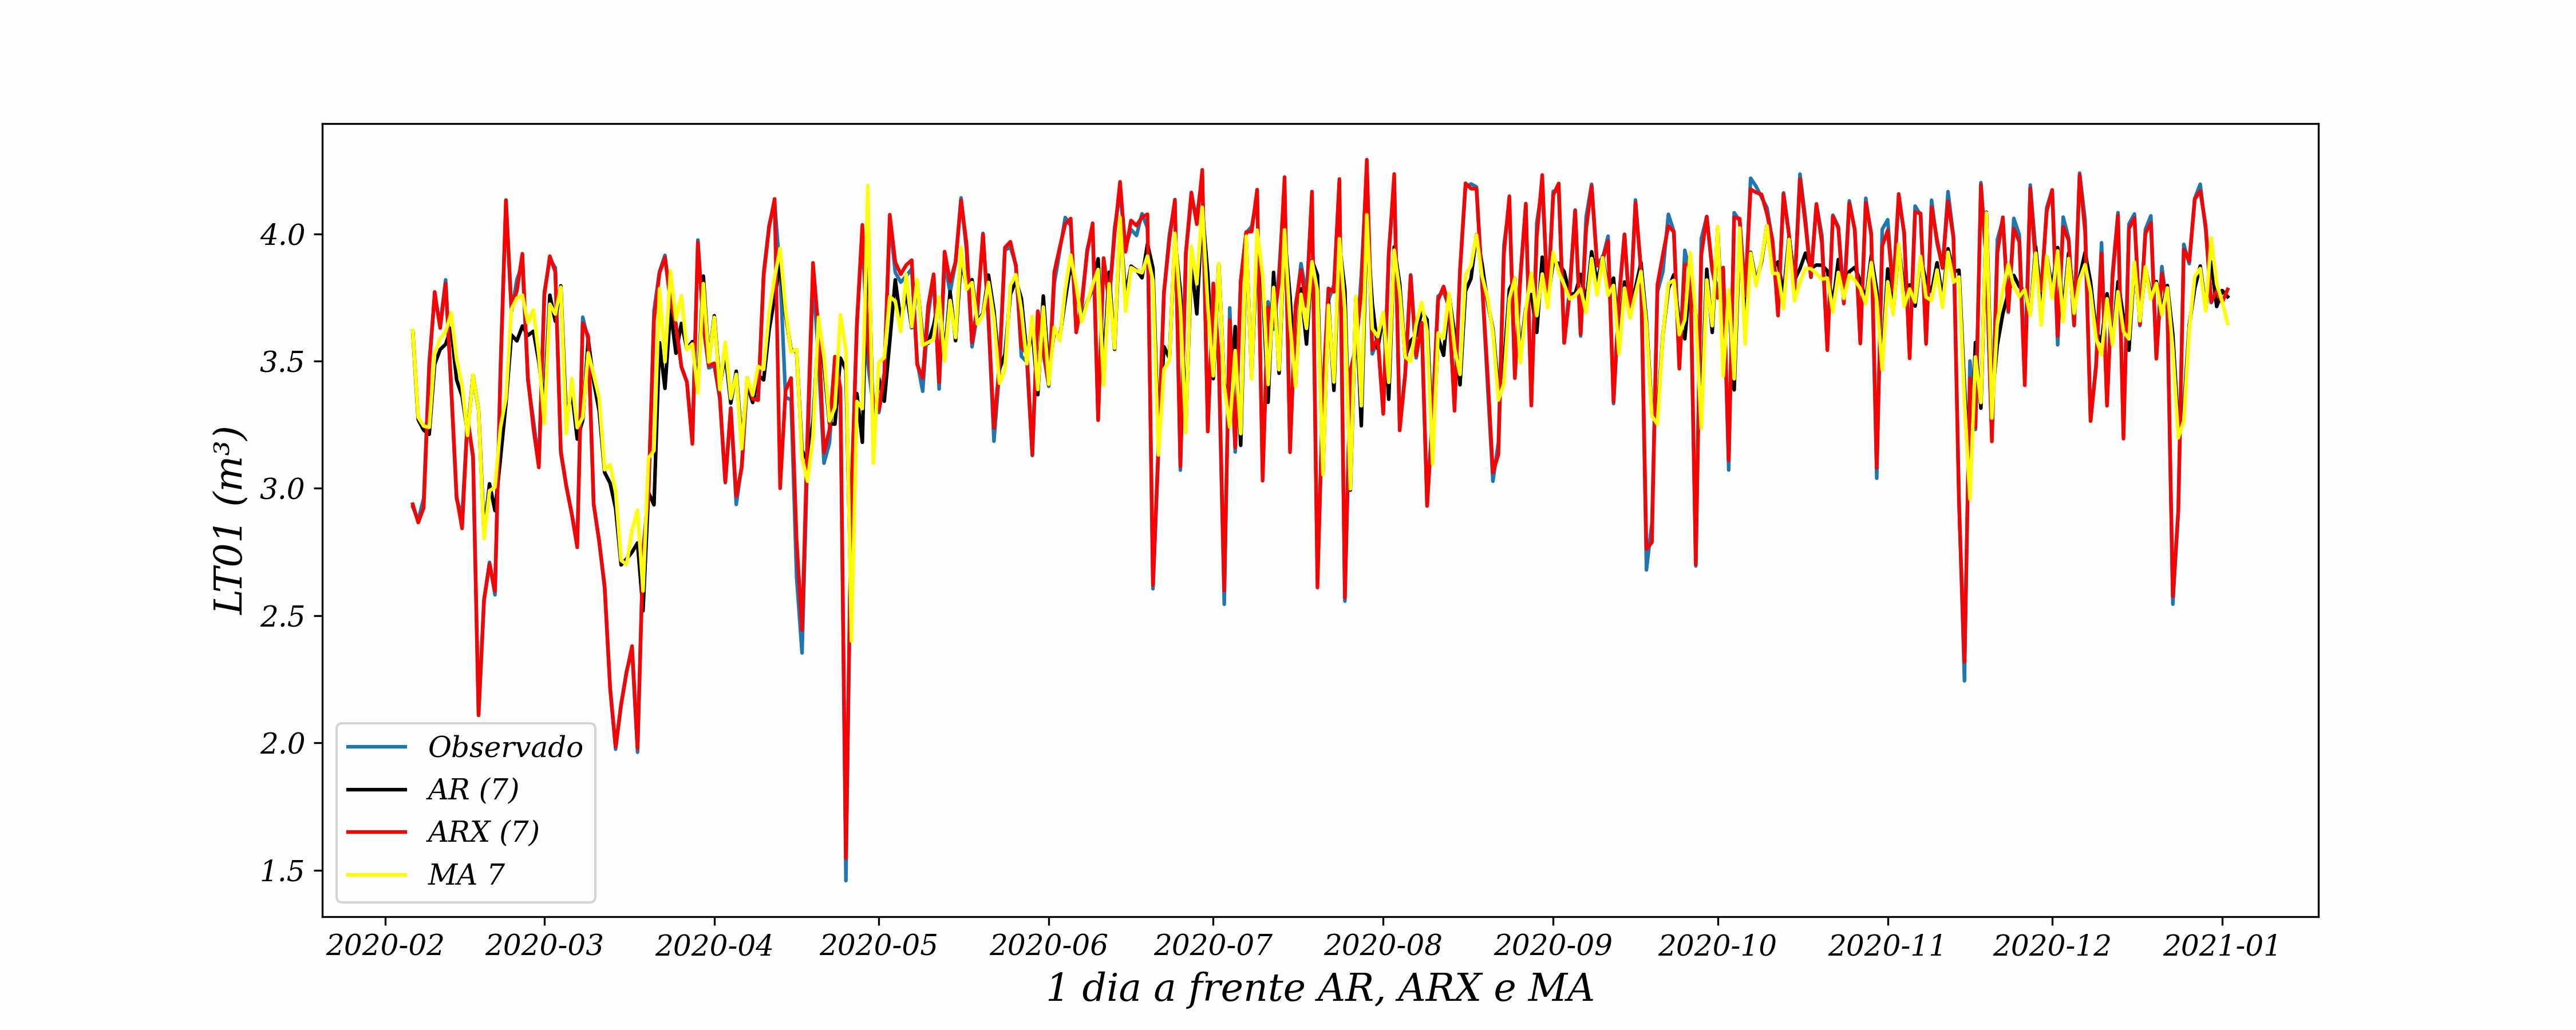
\includegraphics[width=1\linewidth]{Apendices/Figuras/modelagem-24h/1-AR-ARX-MA}
%	
%
%\end{figure}
%
%\begin{figure}[H]
%	\centering
%	\caption{Comparação dos modelos AR, ARX e MA, 7 dias à frente }
%	\label{fig:10-AR-ARX-MA24}
%	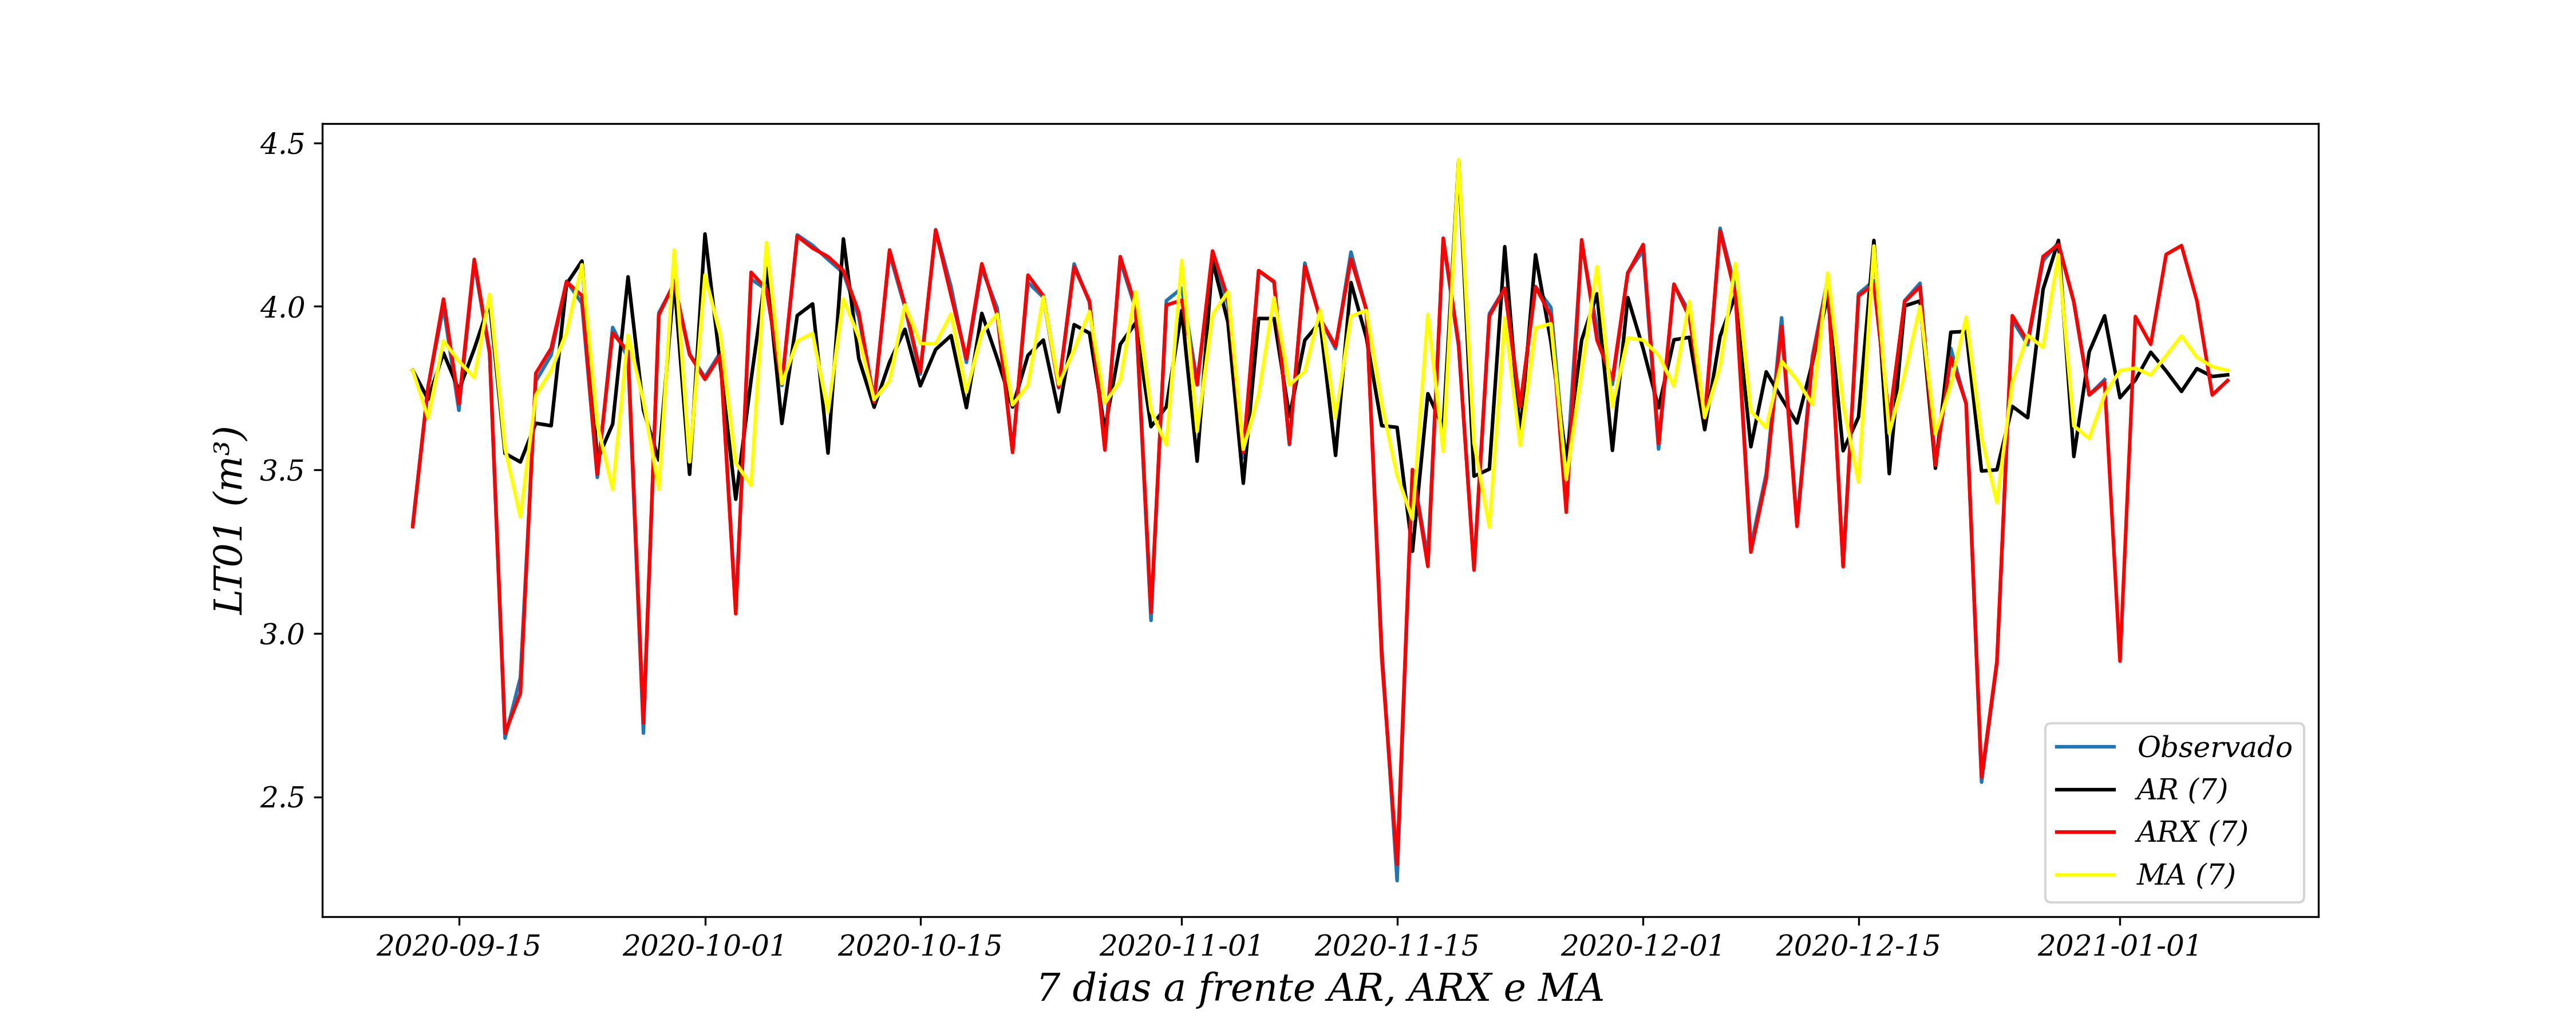
\includegraphics[width=1\linewidth]{Apendices/Figuras/modelagem-24h/7-AR-ARX-MA}
%	
%
%\end{figure}
%
%
%\begin{figure}[H]
%	\centering
%	\caption{Comparação dos modelos AR, ARX e MA, 14 dias à frente }
%	\label{fig:30-AR-ARX-MA24}
%	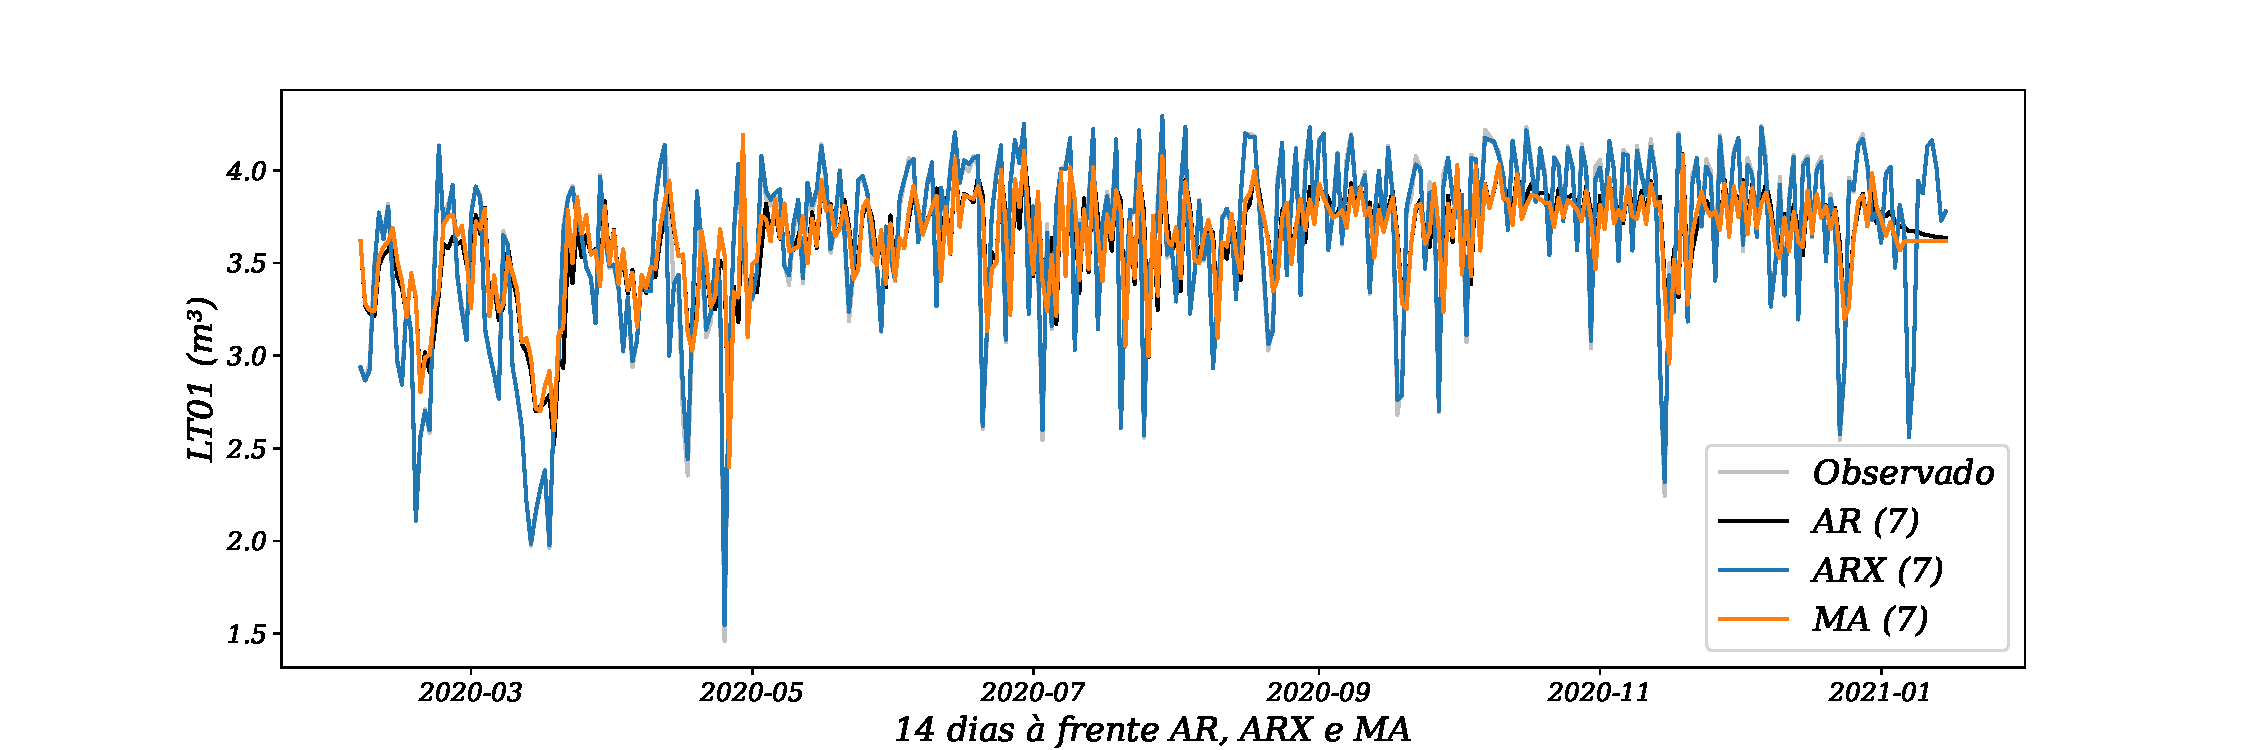
\includegraphics[width=1\linewidth]{Apendices/Figuras/modelagem-24h/14-AR-ARX-MA}
%	
%
%\end{figure}
%
%\begin{figure}[H]
%	\centering
%	\caption{Comparação dos modelos AR, ARX e MA, 30 dias à frente }
%	\label{fig:60-AR-ARX-MA24}
%	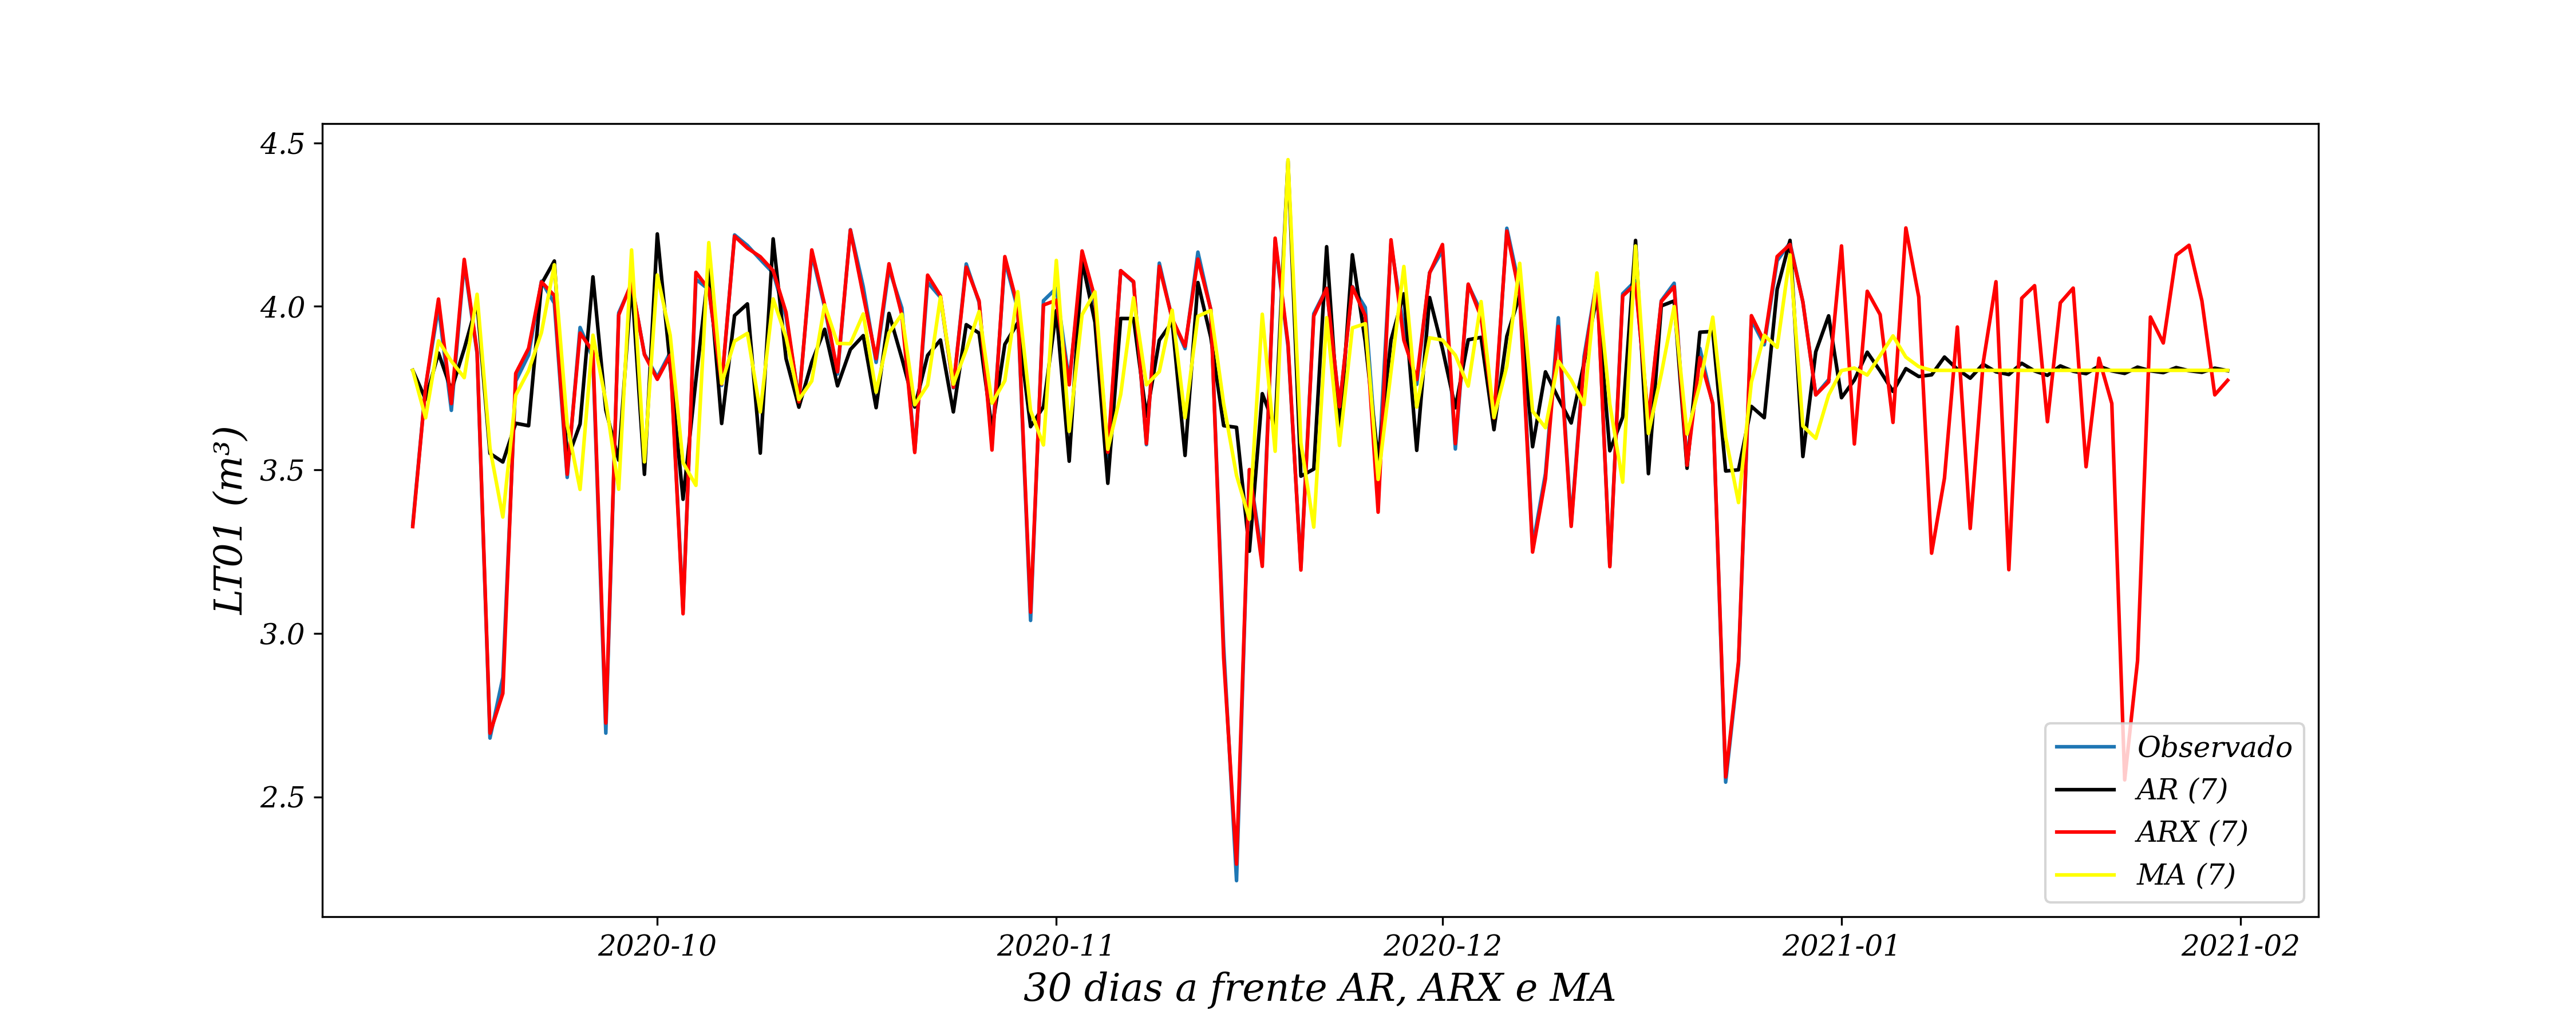
\includegraphics[width=1\linewidth]{Apendices/Figuras/modelagem-24h/30-AR-ARX-MA}
%	
%
%\end{figure}
%


%
%\section{Ap\^endice - Modelos ARMA e ARIMA }\label{sec:armaarima24}
%
%\begin{figure}[H]
%	\centering
%	\caption{Comparação dos modelos ARMA e ARIMA, 1 dia à frente }
%	\label{fig:1-ARMA-ARIMA24}
%	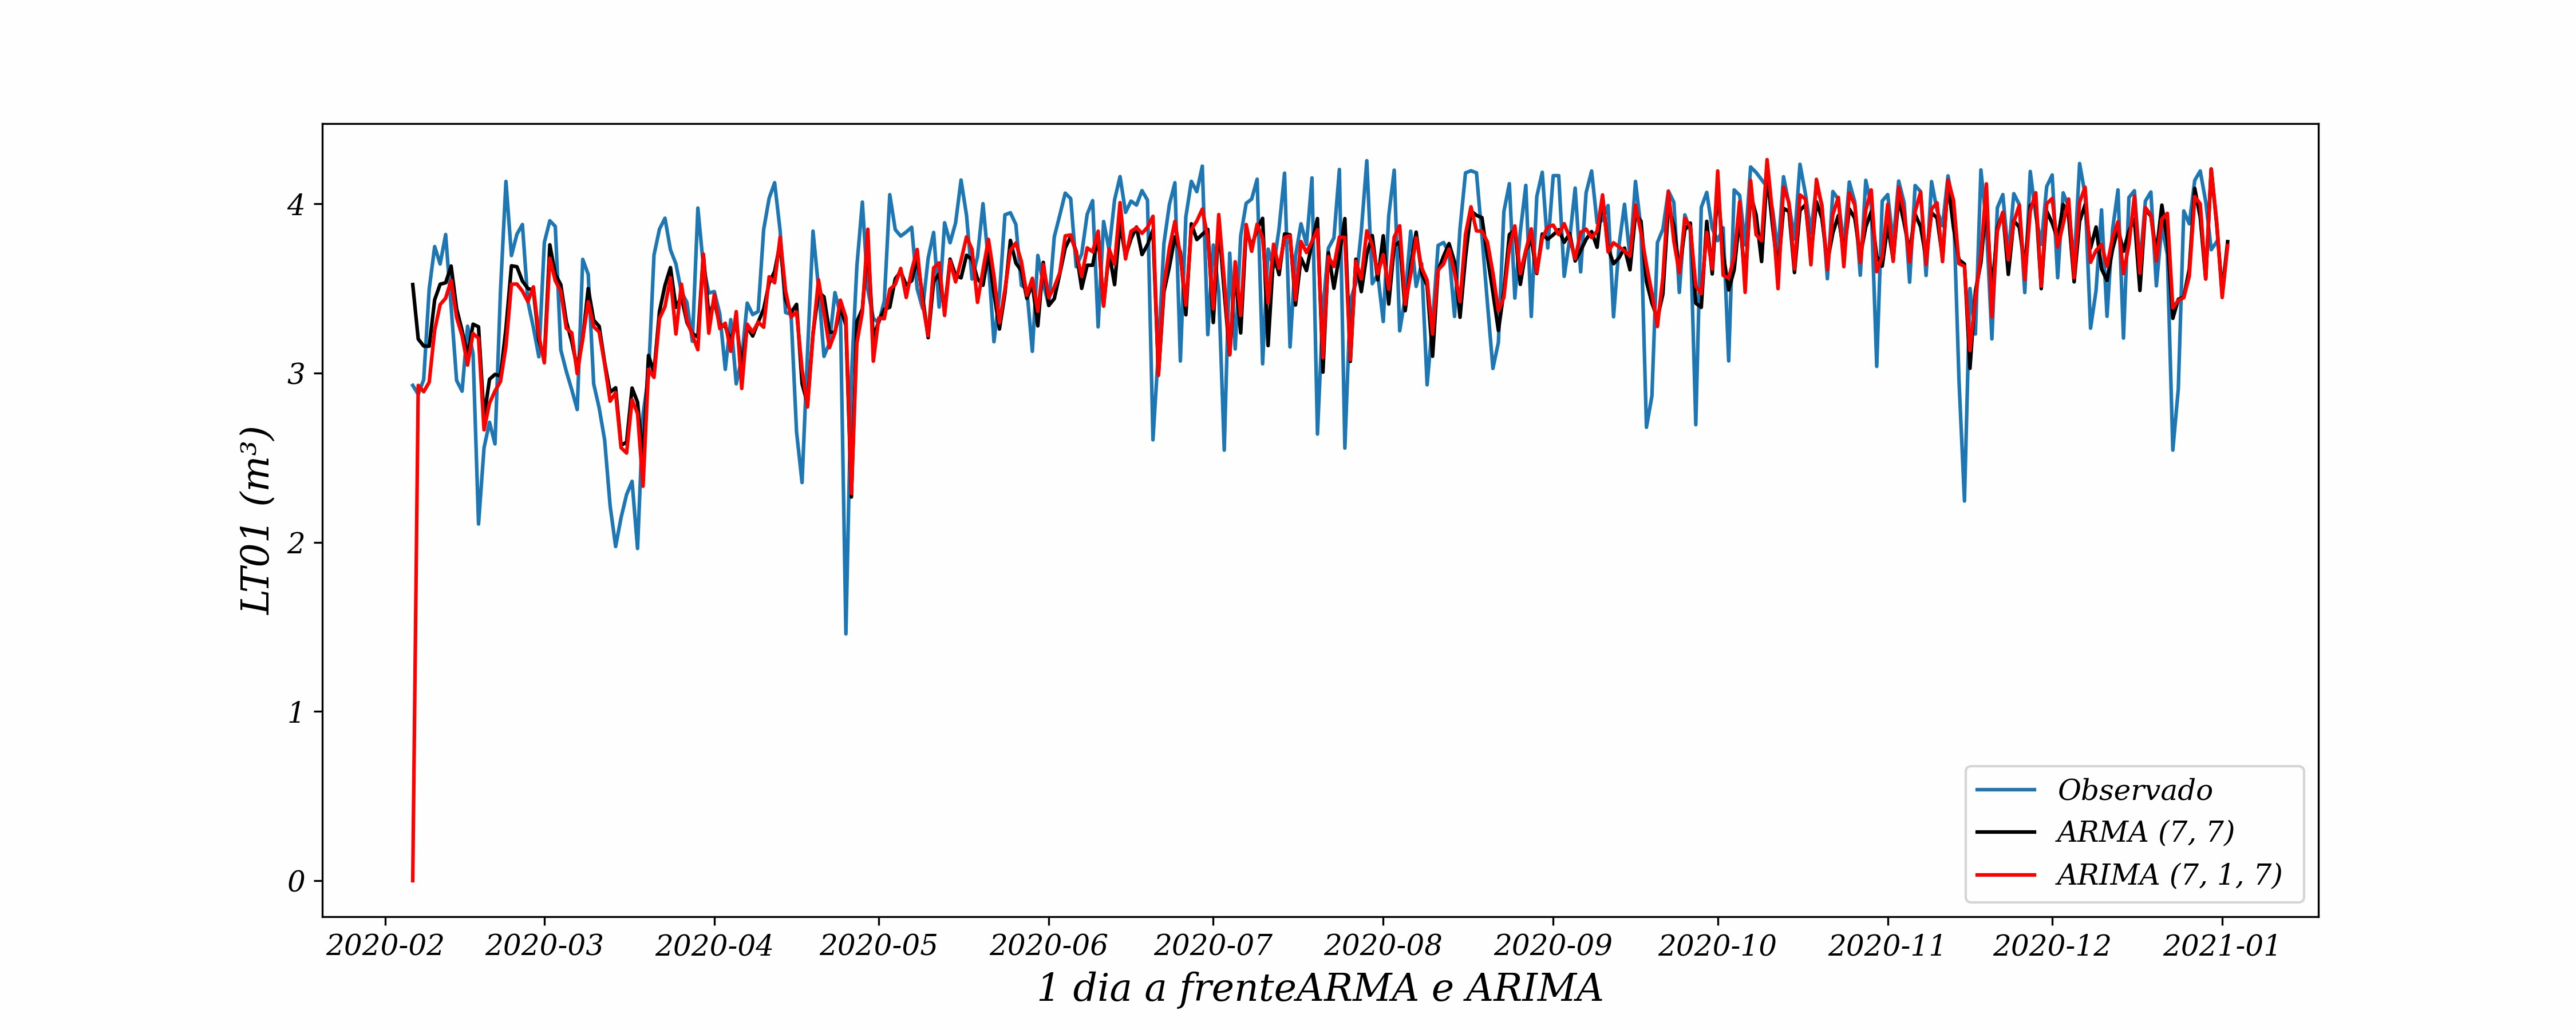
\includegraphics[width=1\linewidth]{Apendices/Figuras/modelagem-24h/1-ARMA-ARIMA}
%	
%
%\end{figure}
%
%\begin{figure}[H]
%	\centering
%	\caption{Comparação dos modelos ARMA e ARIMA, 7 dias à frente }
%	\label{fig:10-ARMA-ARIMA24}
%	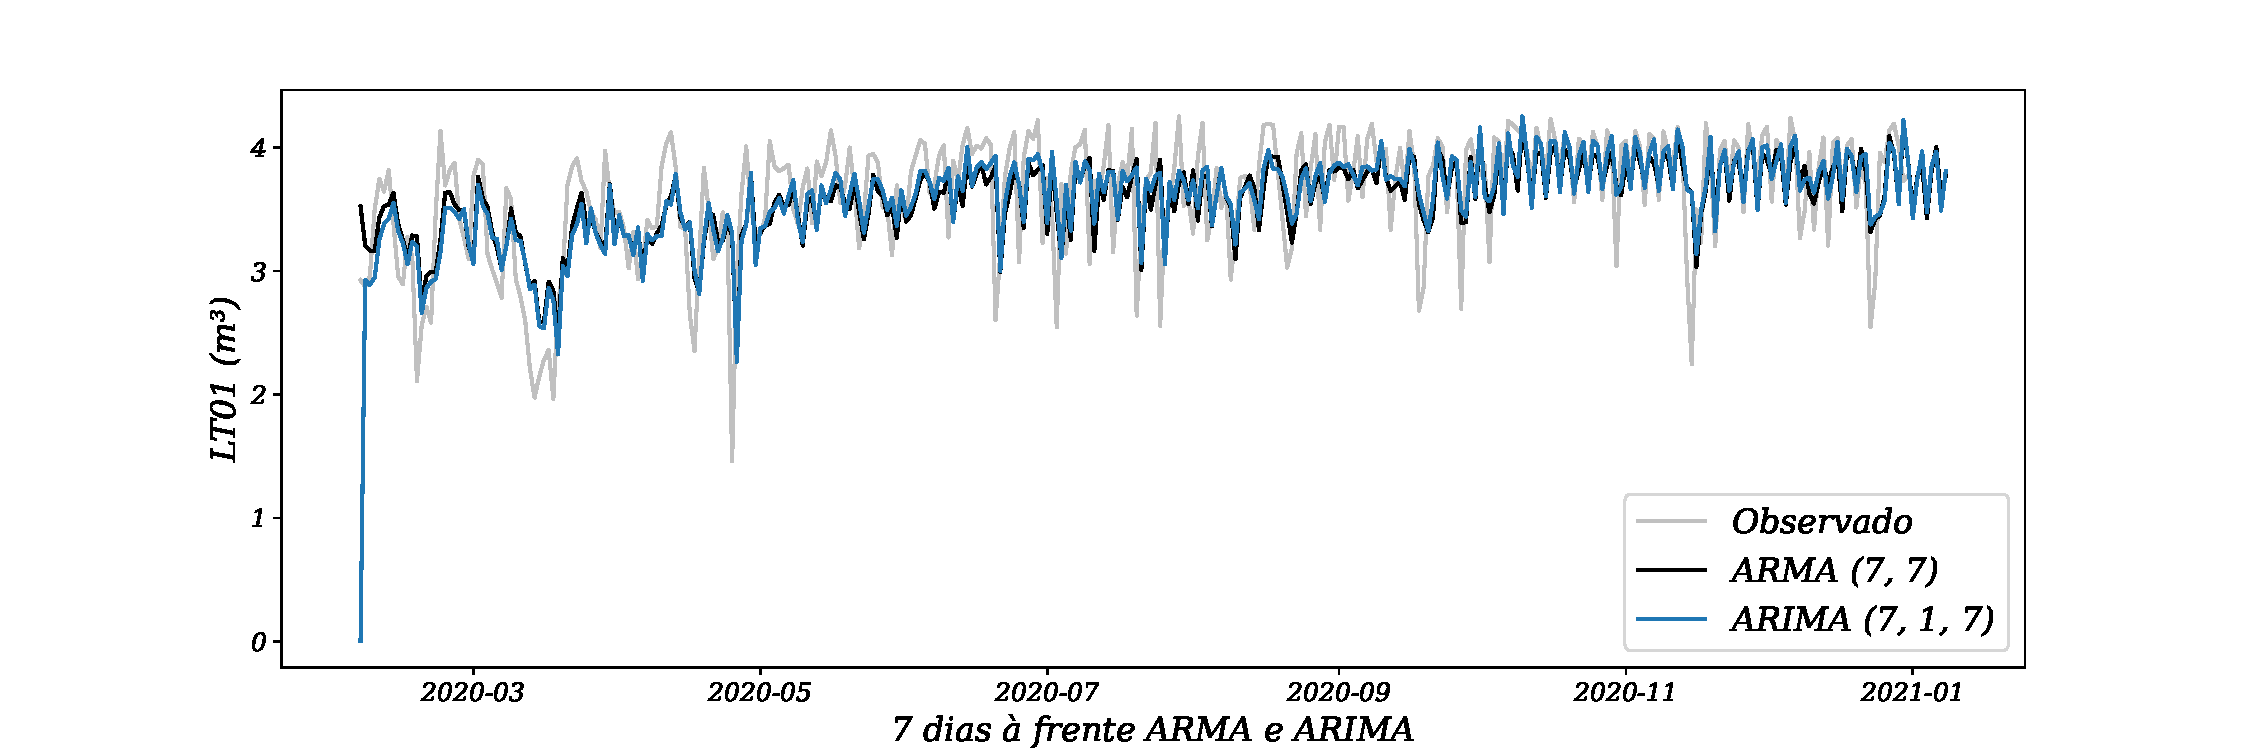
\includegraphics[width=1\linewidth]{Apendices/Figuras/modelagem-24h/7-ARMA-ARIMA}
%	
%
%\end{figure}
%
%
%\begin{figure}[H]
%	\centering
%	\caption{Comparação dos modelos ARMA e ARIMA, 14 dias à frente }
%	\label{fig:30-ARMA-ARIMA24}
%	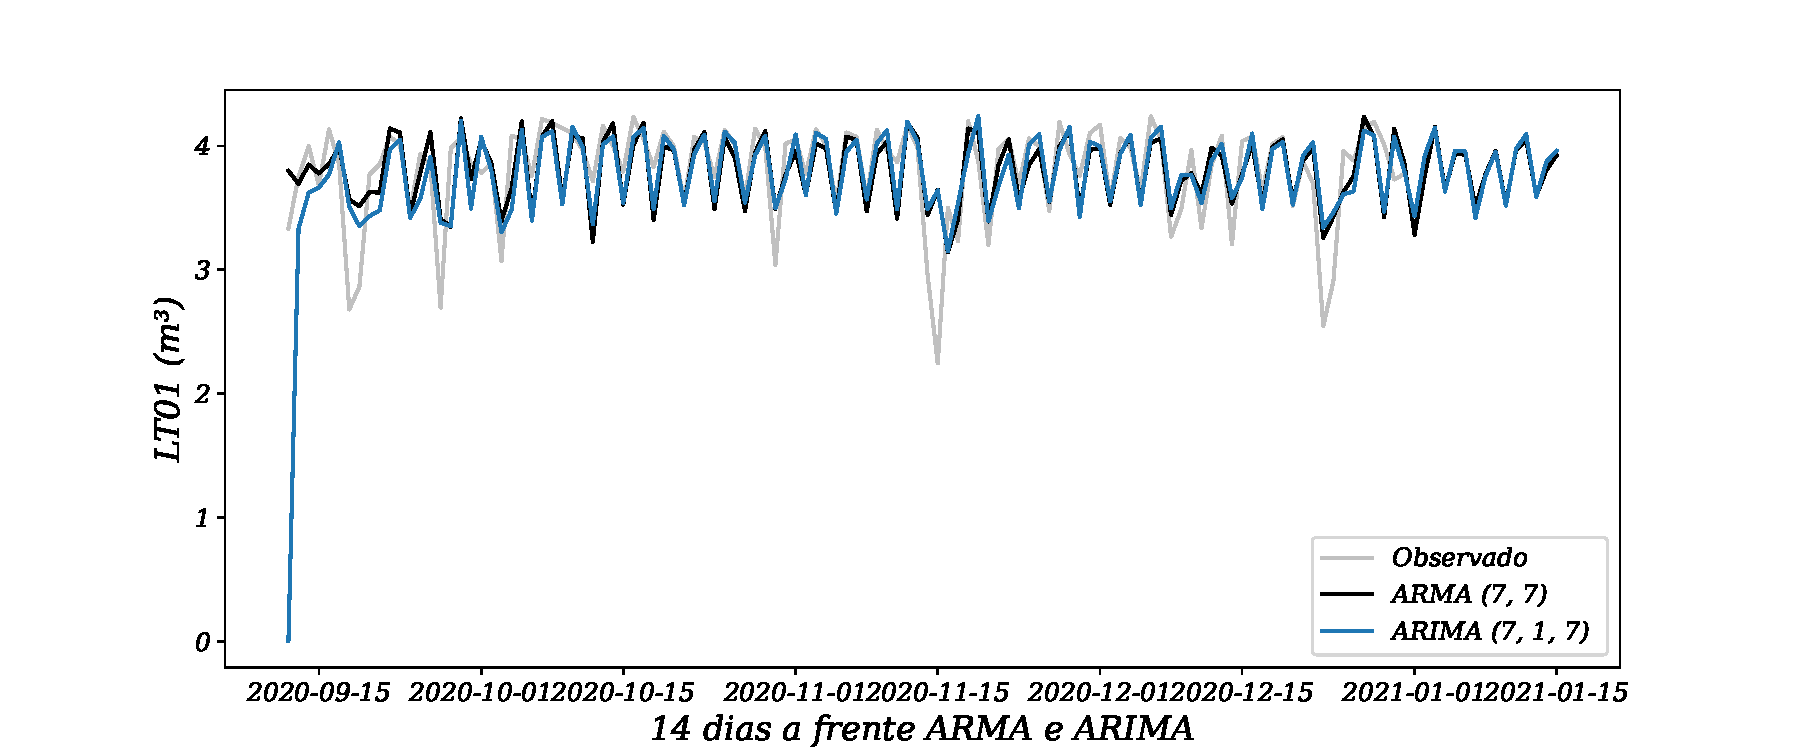
\includegraphics[width=1\linewidth]{Apendices/Figuras/modelagem-24h/14-ARMA-ARIMA}
%
%\end{figure}
%
%\begin{figure}[H]
%	\centering
%	\caption{Comparação dos modelos ARMA e ARIMA, 30 dias à frente }
%	\label{fig:60-ARMA-ARIMA24}
%	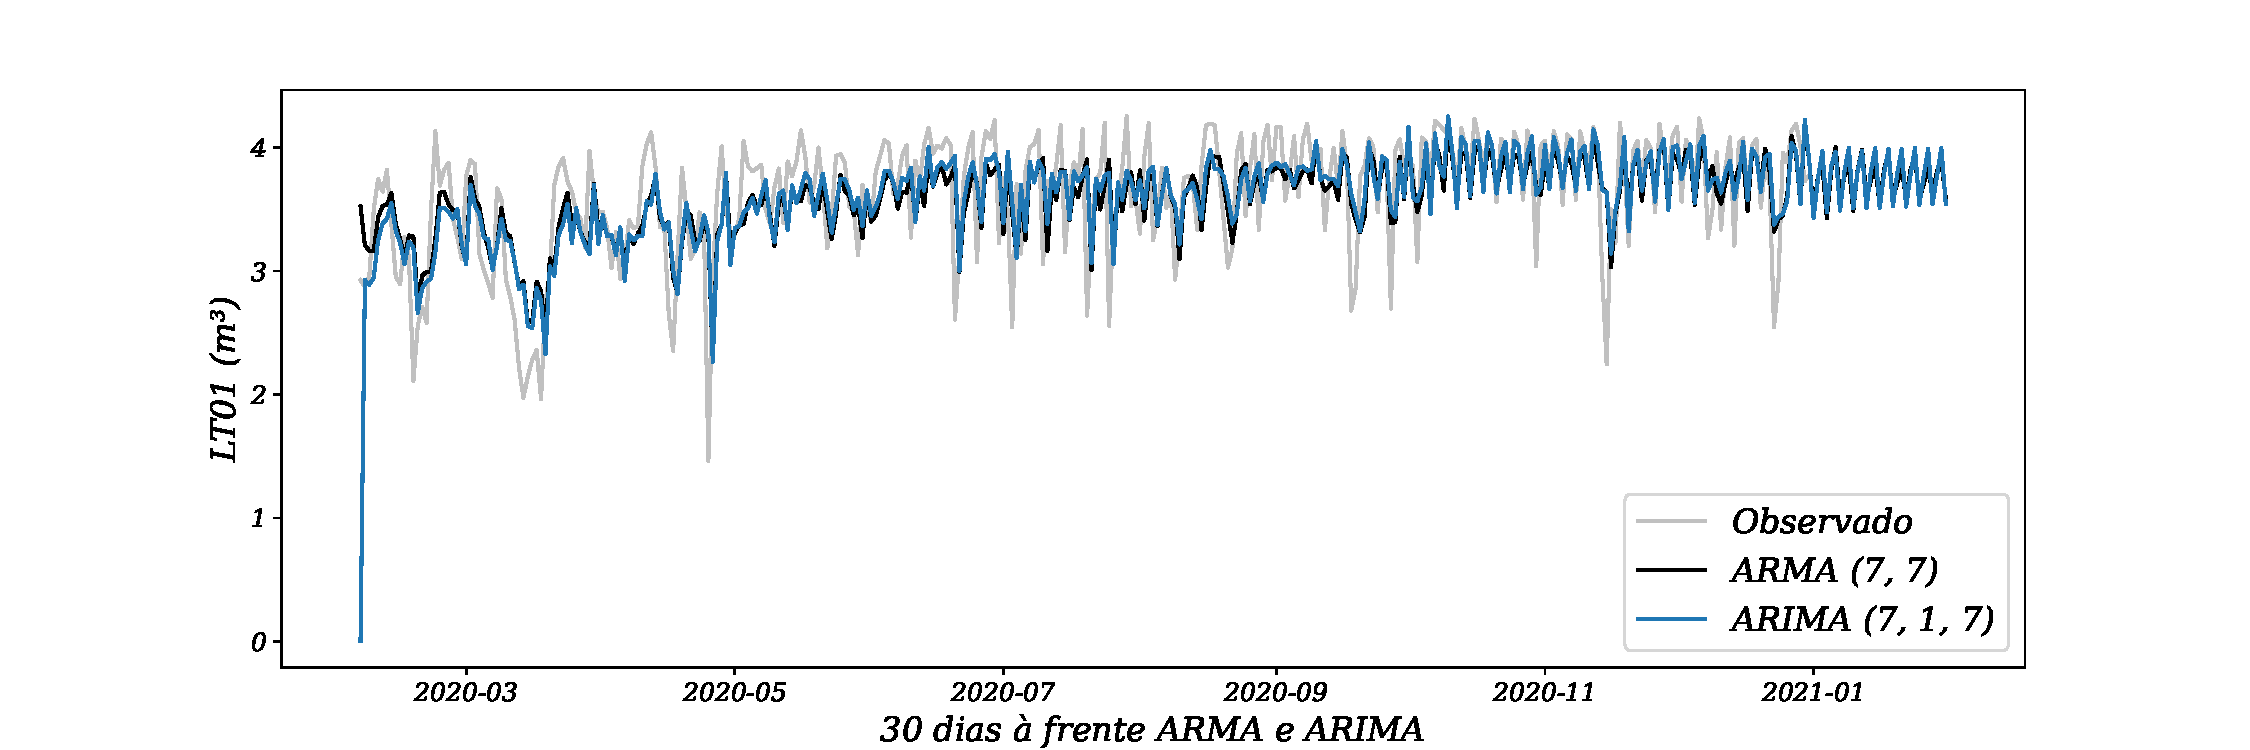
\includegraphics[width=1\linewidth]{Apendices/Figuras/modelagem-24h/30-ARMA-ARIMA}
%	
%
%\end{figure}


\section{Ap\^endice - Modelos ARIMAX, SARIMA e SARIMAX }\label{sec:arimaxsarimasarimax24}

\begin{figure}[H]
	\centering
	\caption{Comparação dos modelos ARIMAX, SARIMA e SARIMAX, 1 dia à frente }
	\label{fig:1-ARIMAX-SARIMA-SARIMAX24}
	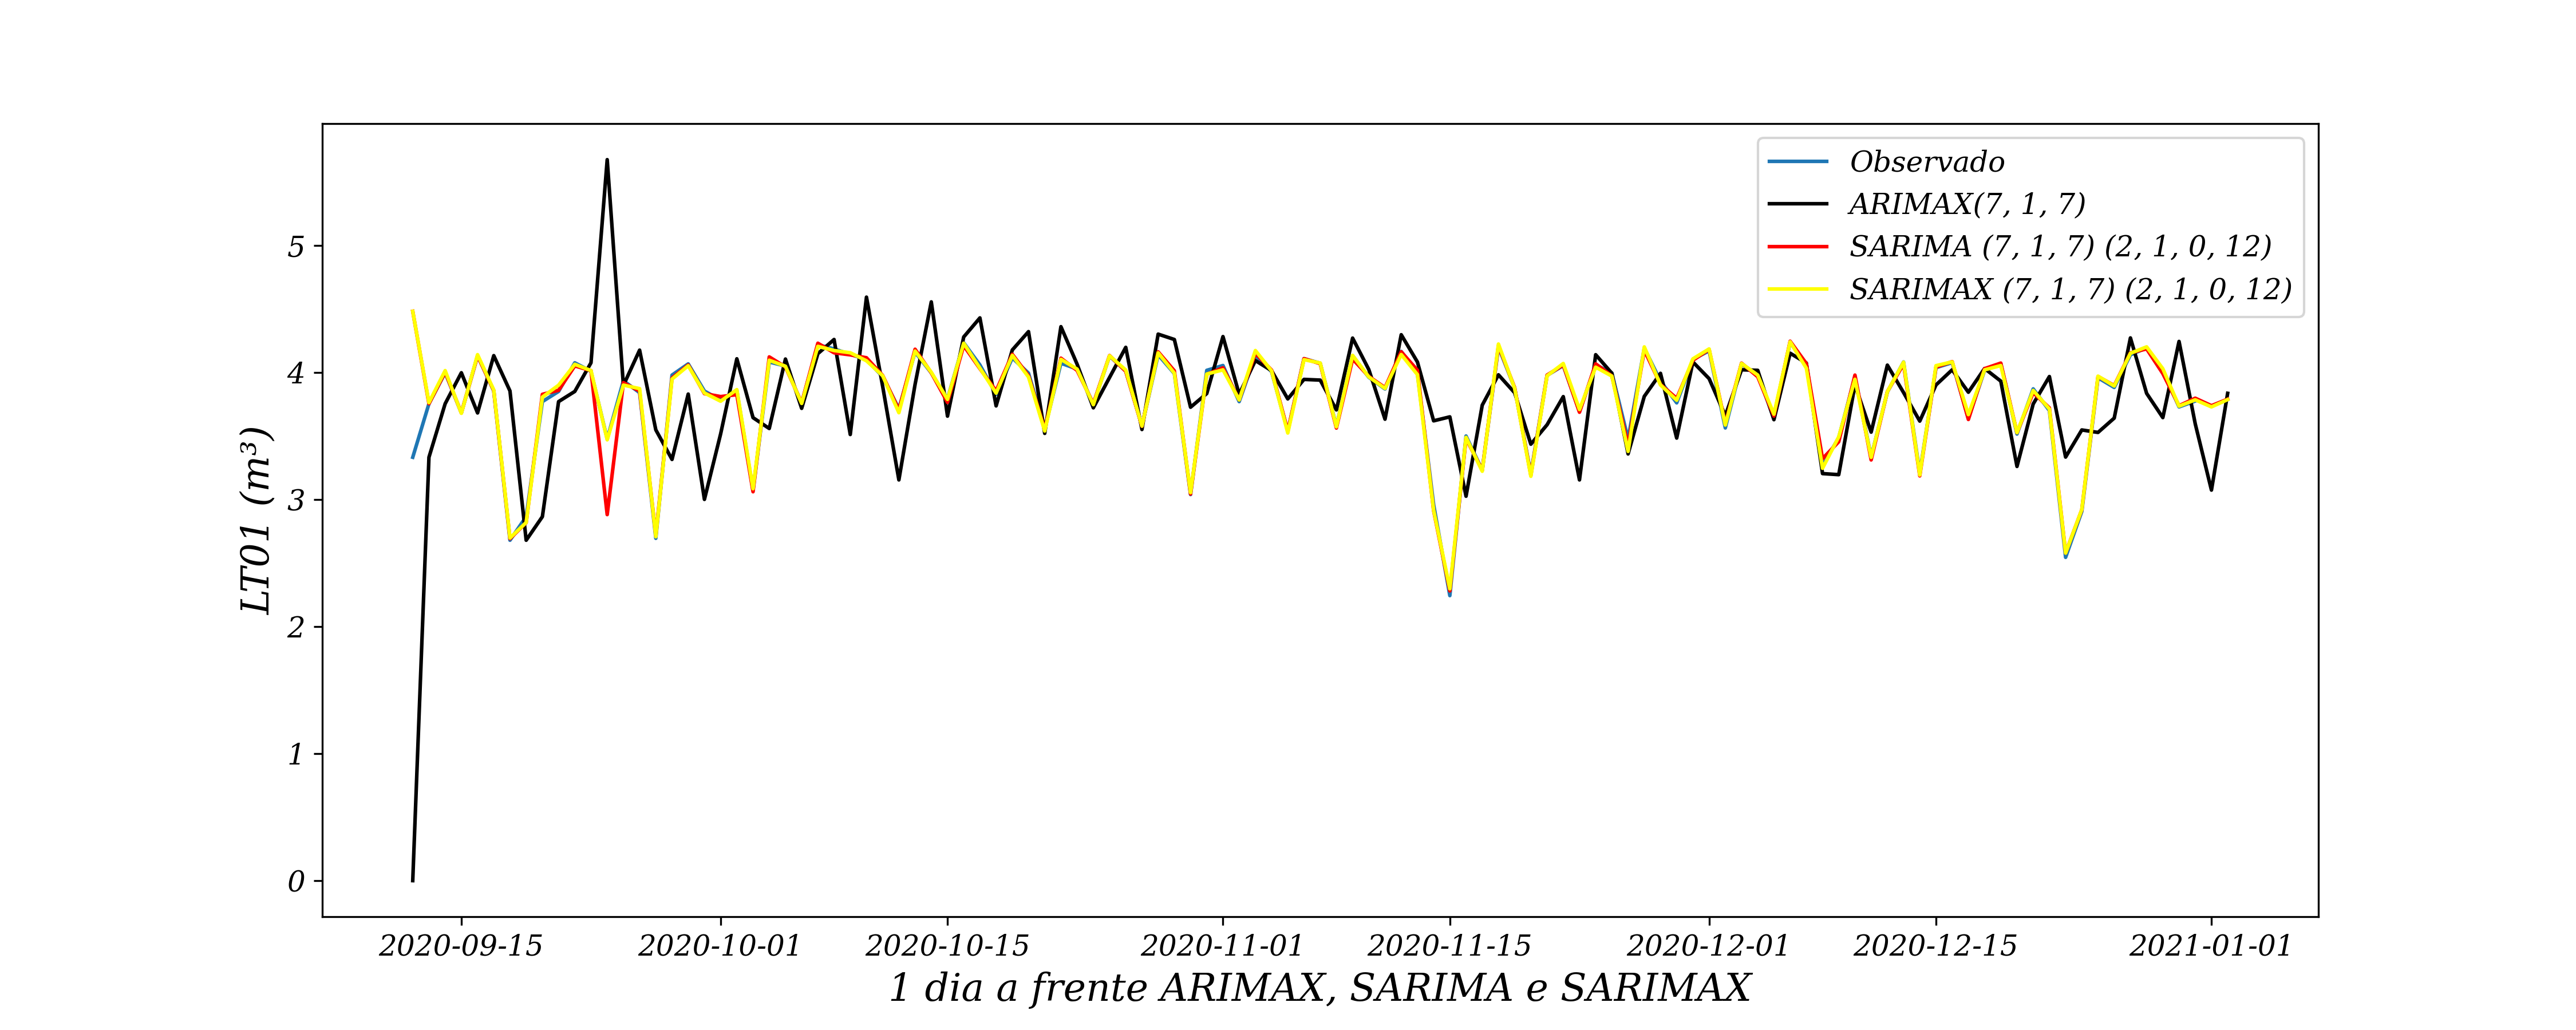
\includegraphics[width=1\linewidth]{Apendices/Figuras/modelagem-24h/1-ARIMAX-SARIMA-SARIMAX}
	
		\fonte{Elaboração própria a partir de dados da SANEPAR (2018 a 2020)}
\end{figure}

\begin{figure}[H]
	\centering
	\caption{Comparação dos modelos ARIMAX, SARIMA e SARIMAX, 7 dias à frente }
	\label{fig:10-ARIMAX-SARIMA-SARIMAX24}
	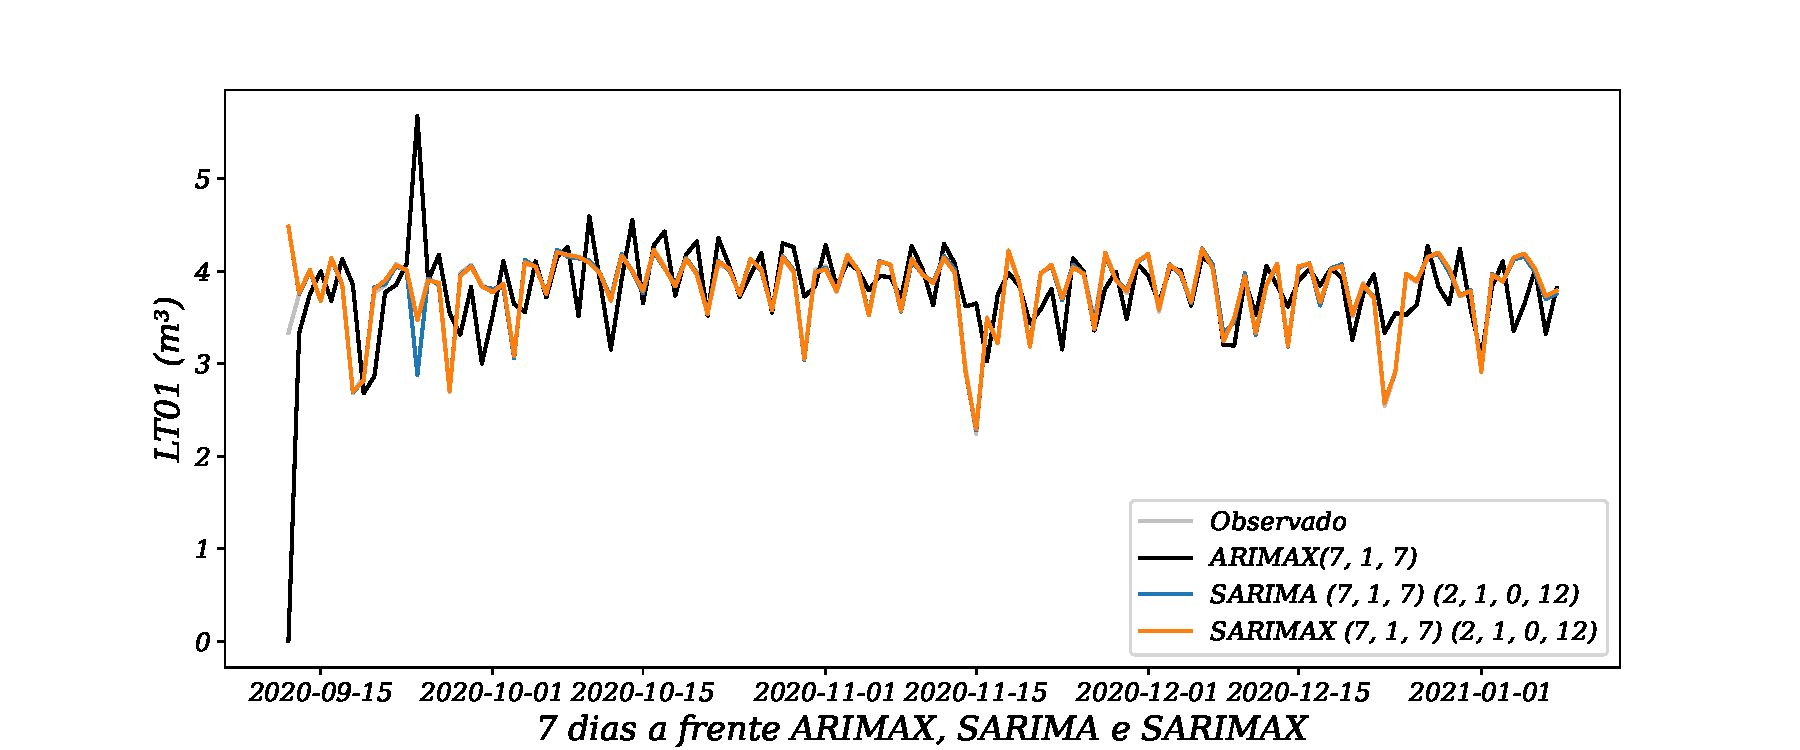
\includegraphics[width=1\linewidth]{Apendices/Figuras/modelagem-24h/7-ARIMAX-SARIMA-SARIMAX}
	
	\fonte{Elaboração própria a partir de dados da SANEPAR (2018 a 2020)}
\end{figure}


\begin{figure}[H]
	\centering
	\caption{Comparação dos modelos ARIMAX, SARIMA e SARIMAX, 14 dias à frente }
	\label{fig:30-ARIMAX-SARIMA-SARIMAX24}
	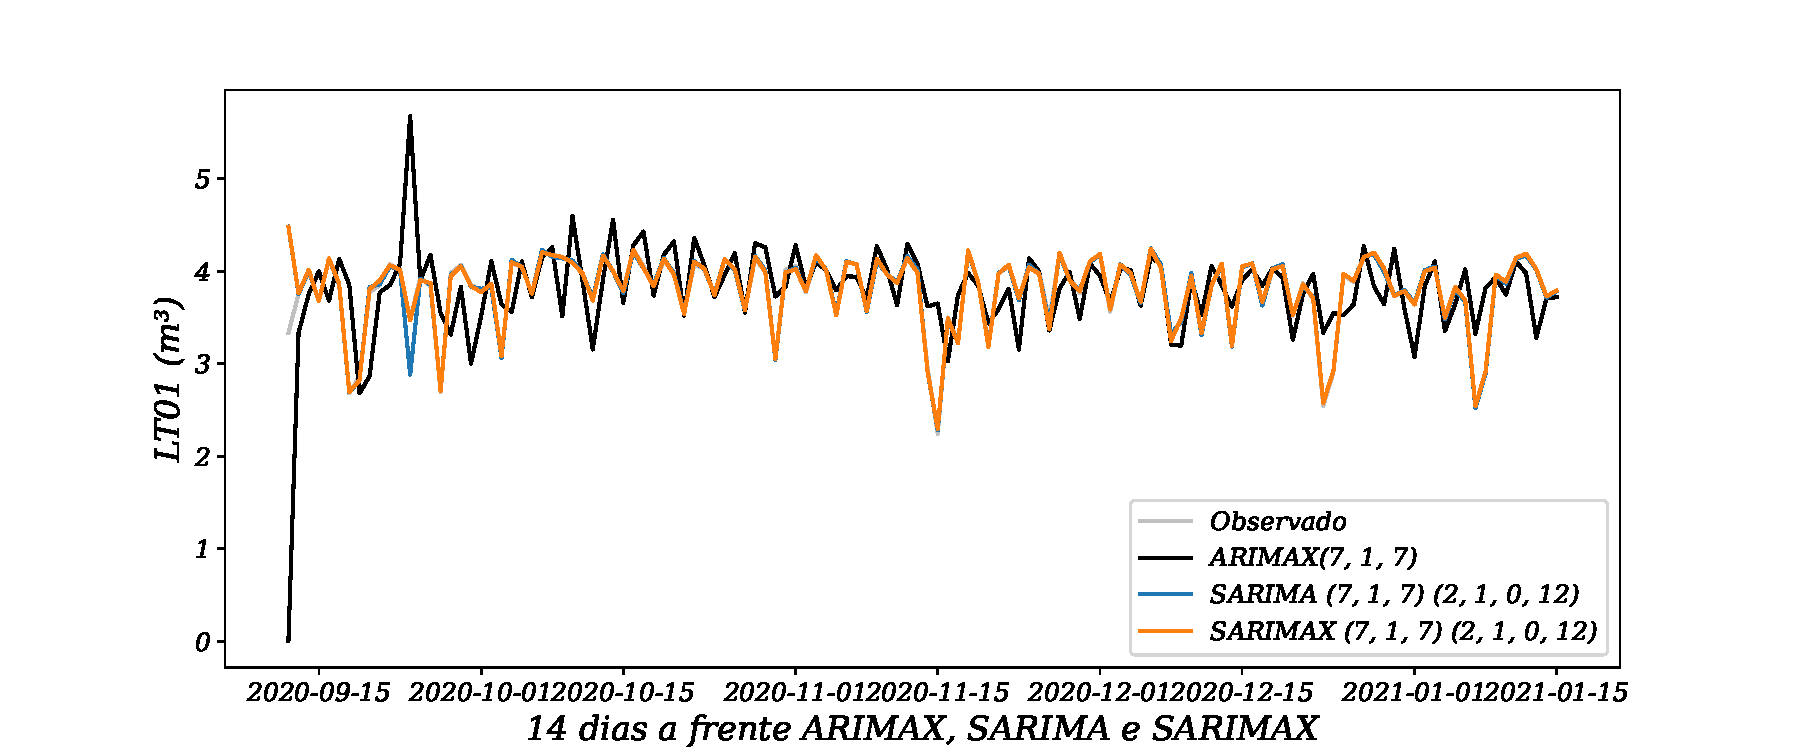
\includegraphics[width=1\linewidth]{Apendices/Figuras/modelagem-24h/14-ARIMAX-SARIMA-SARIMAX}
	
	\fonte{Elaboração própria a partir de dados da SANEPAR (2018 a 2020)}
\end{figure}

\begin{figure}[H]
	\centering
	\caption{Comparação dos modelos ARIMAX, SARIMA e SARIMAX, 30 dias à frente }
	\label{fig:60-ARIMAX-SARIMA-SARIMAX24}
	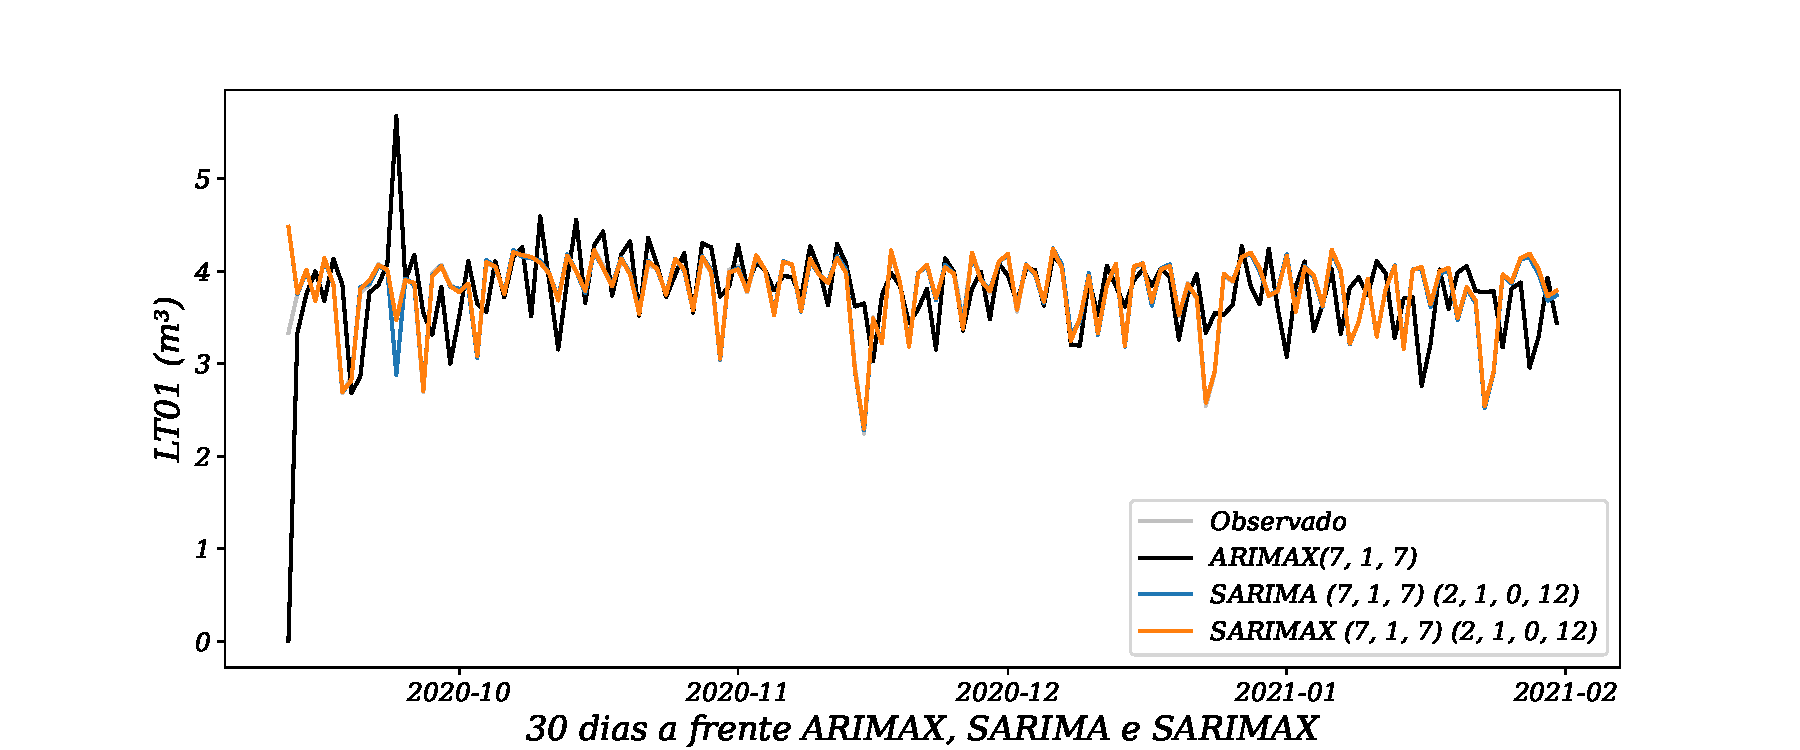
\includegraphics[width=1\linewidth]{Apendices/Figuras/modelagem-24h/30-ARIMAX-SARIMA-SARIMAX}
	
	\fonte{Elaboração própria a partir de dados da SANEPAR (2018 a 2020)}
\end{figure}

\newpage

\section{Ap\^endice - Modelos RNN e Prophet }\label{sec:rnnprophet}

\begin{figure}[H]
	\centering
	\caption{A rede neural recorrente (RNN) com todos os horizontes }
	\label{fig:rnn}
	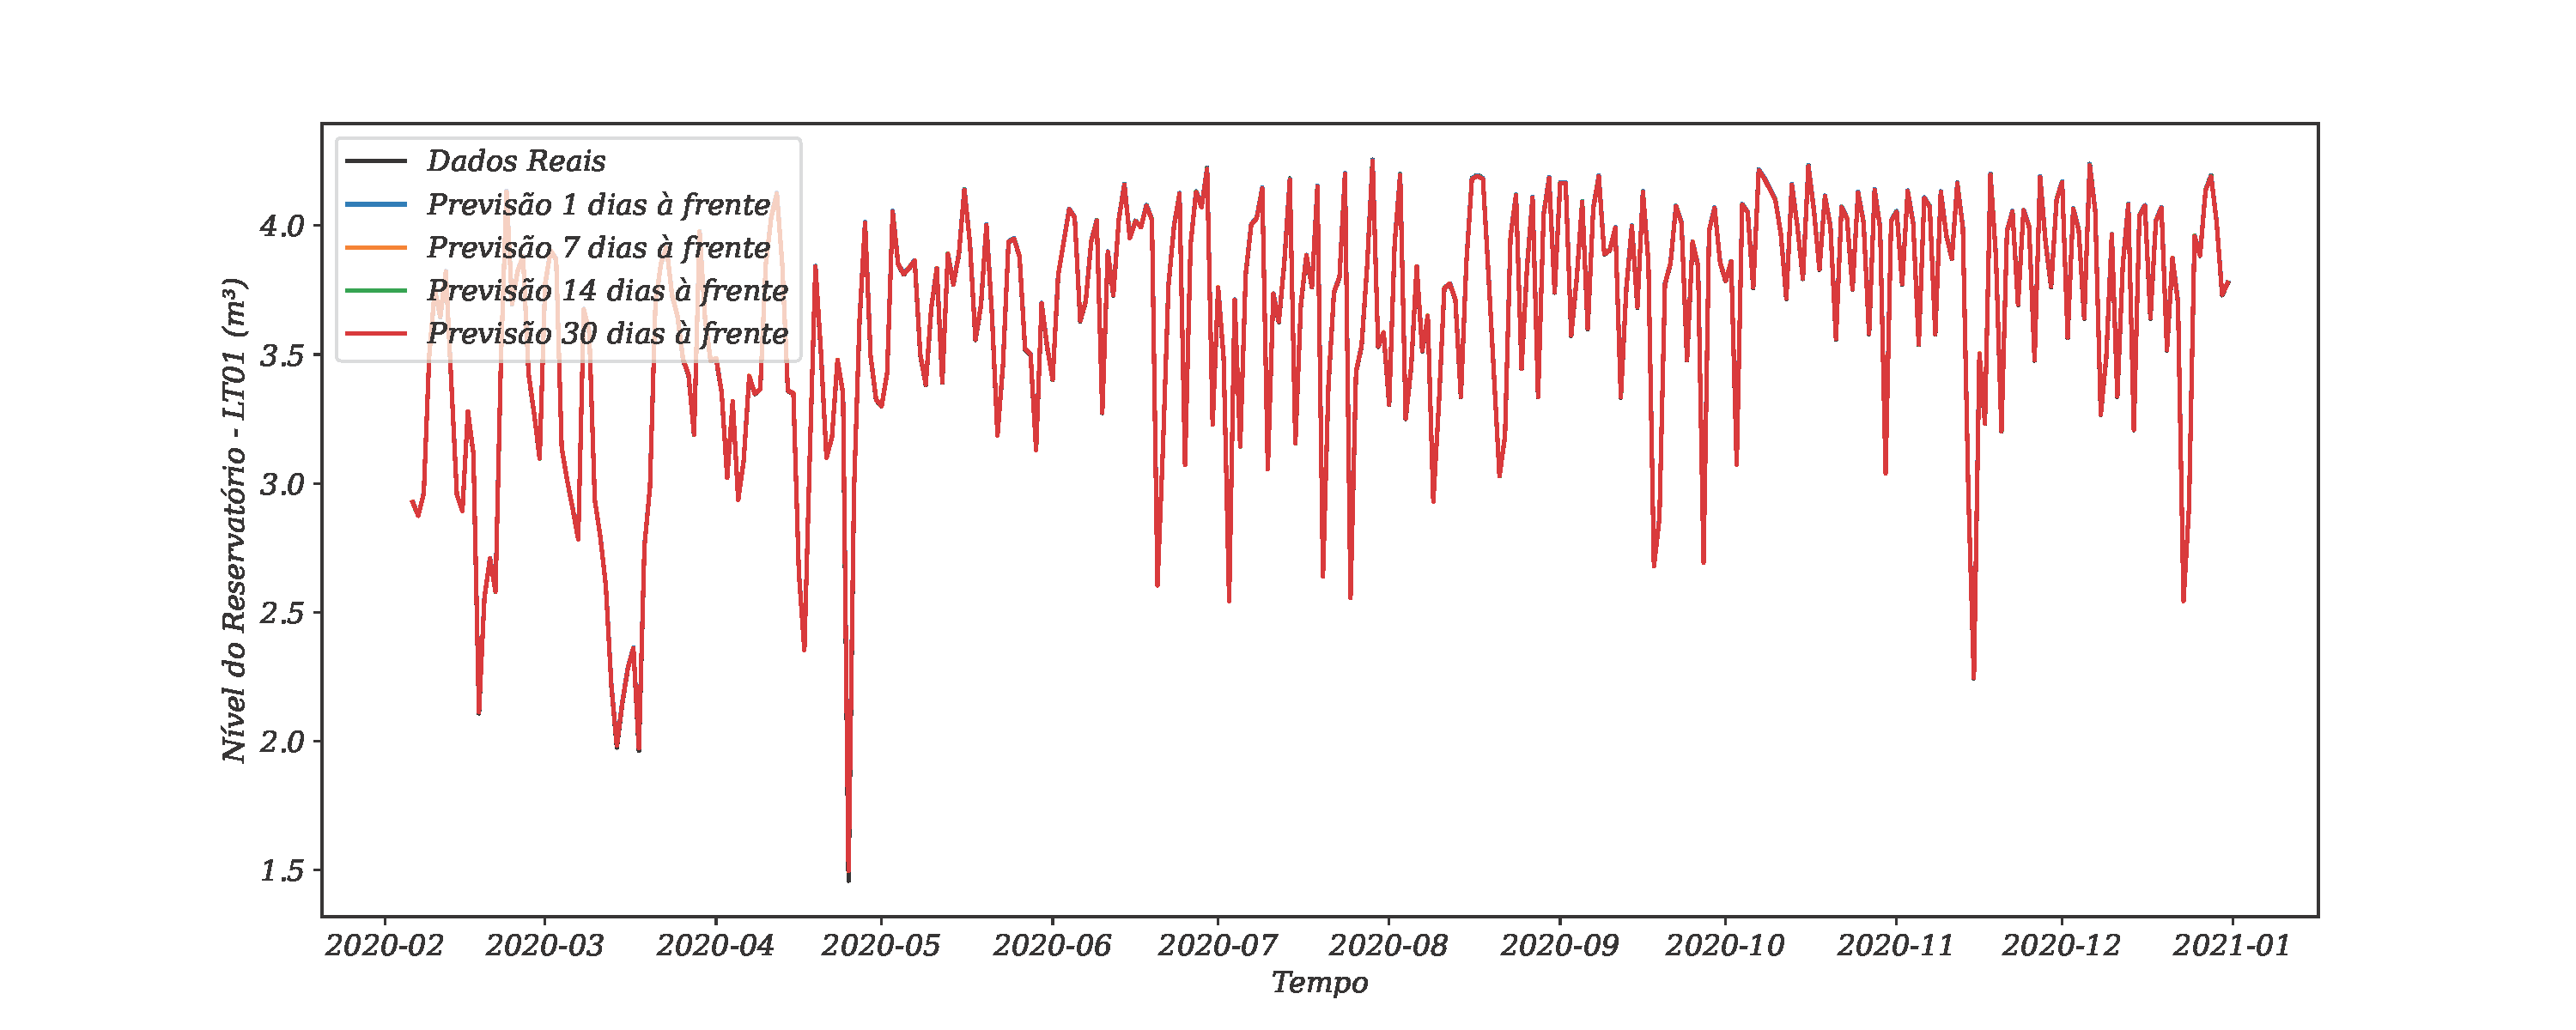
\includegraphics[width=1\linewidth]{Apendices/Figuras/modelagem-24h/RNN}
	
	\fonte{Elaboração própria a partir de dados da SANEPAR (2018 a 2020)}
\end{figure}

\begin{figure}[H]
	\centering
	\caption{Previsões do Modelo Prophet para Diferentes Horizontes}
	\label{fig:prophet}
	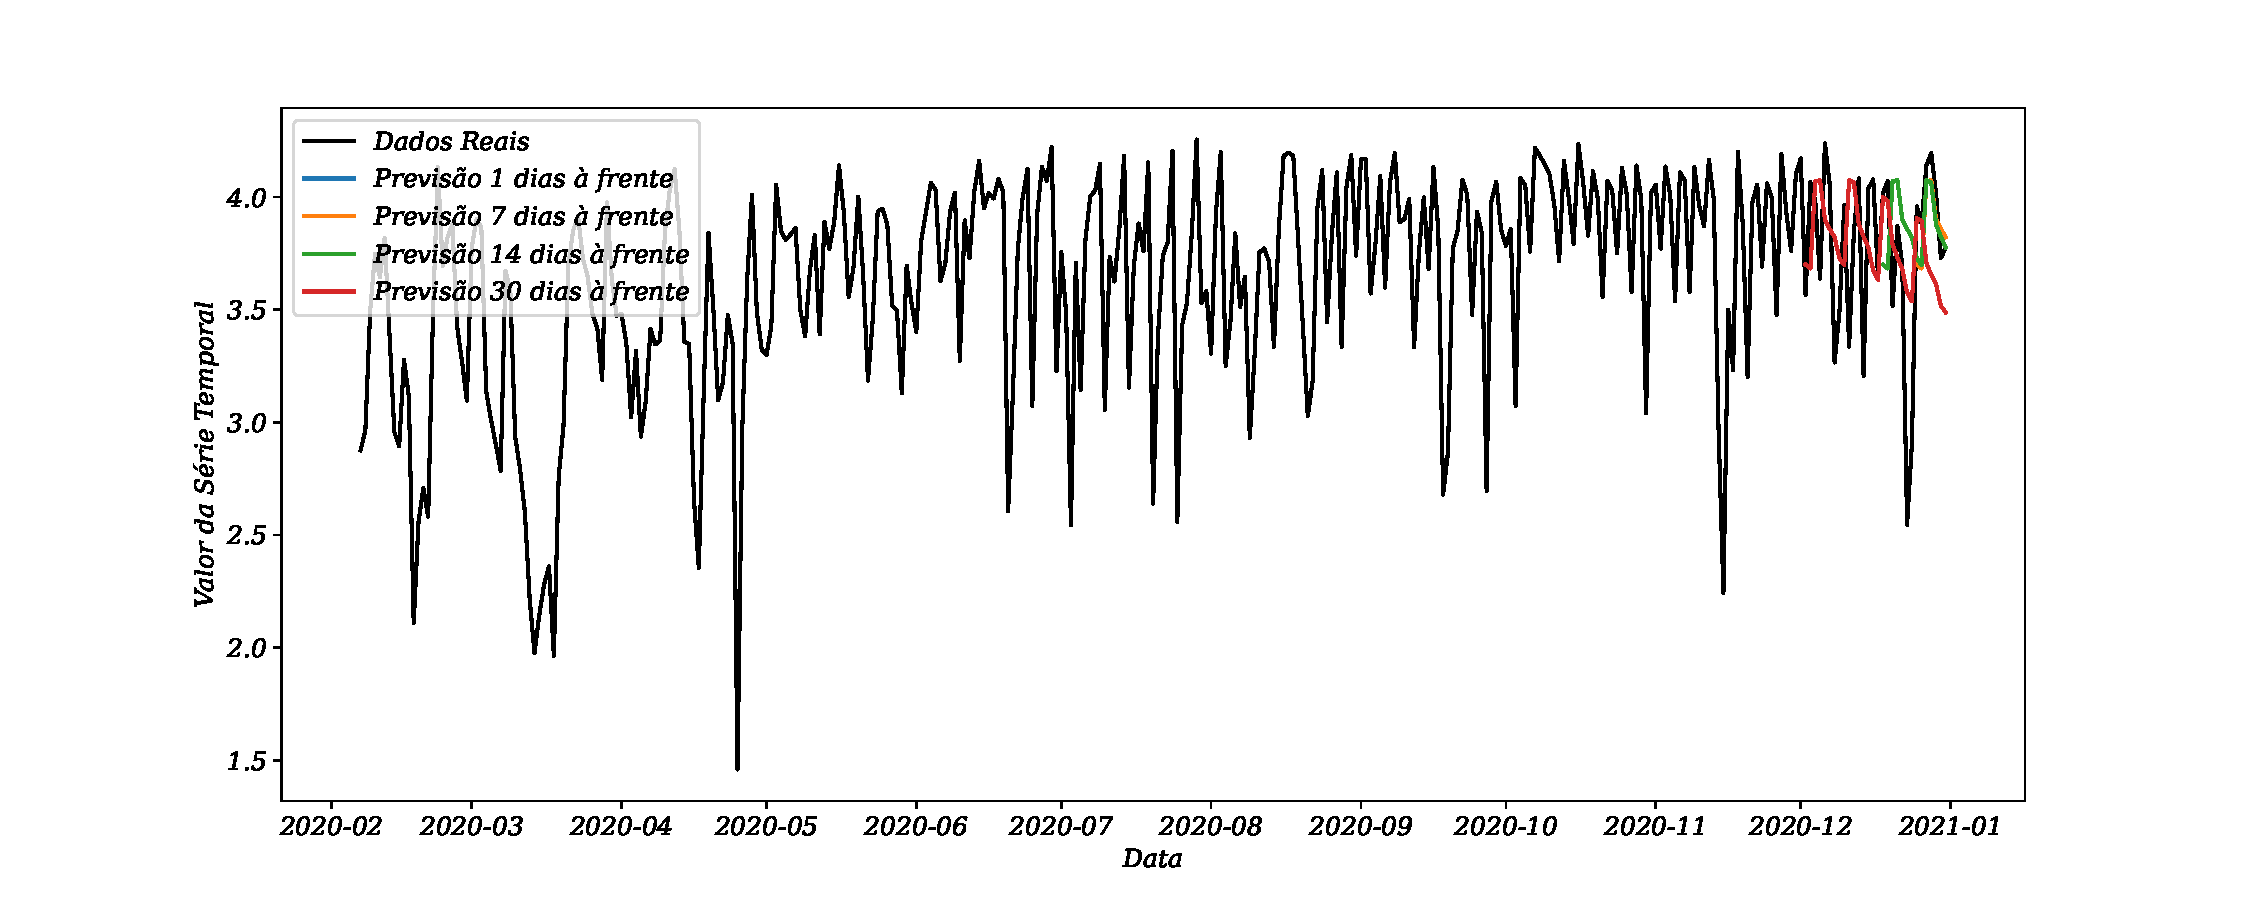
\includegraphics[width=1\linewidth]{Apendices/Figuras/modelagem-24h/prophet}
	
	\fonte{Elaboração própria a partir de dados da SANEPAR (2018 a 2020)}
\end{figure}

%
\section{Ap\^endice - Modelos Regress\~ao linear, XGB Regress\~ao, Ligth GBM Regress\~ao e Regress\~ao de Floresta Aleat\'oria 24h}\label{sec:lrxgblgbmrf24}

\begin{figure}[H]
	\centering
	\caption{Comparação dos modelos Regressão linear, XGB Regressão, Ligth GBM Regressão e Regressão de Floresta Aleatória, 1 dia a frente }
	\label{fig:1-LR-XGB-LGBM-RF24}
	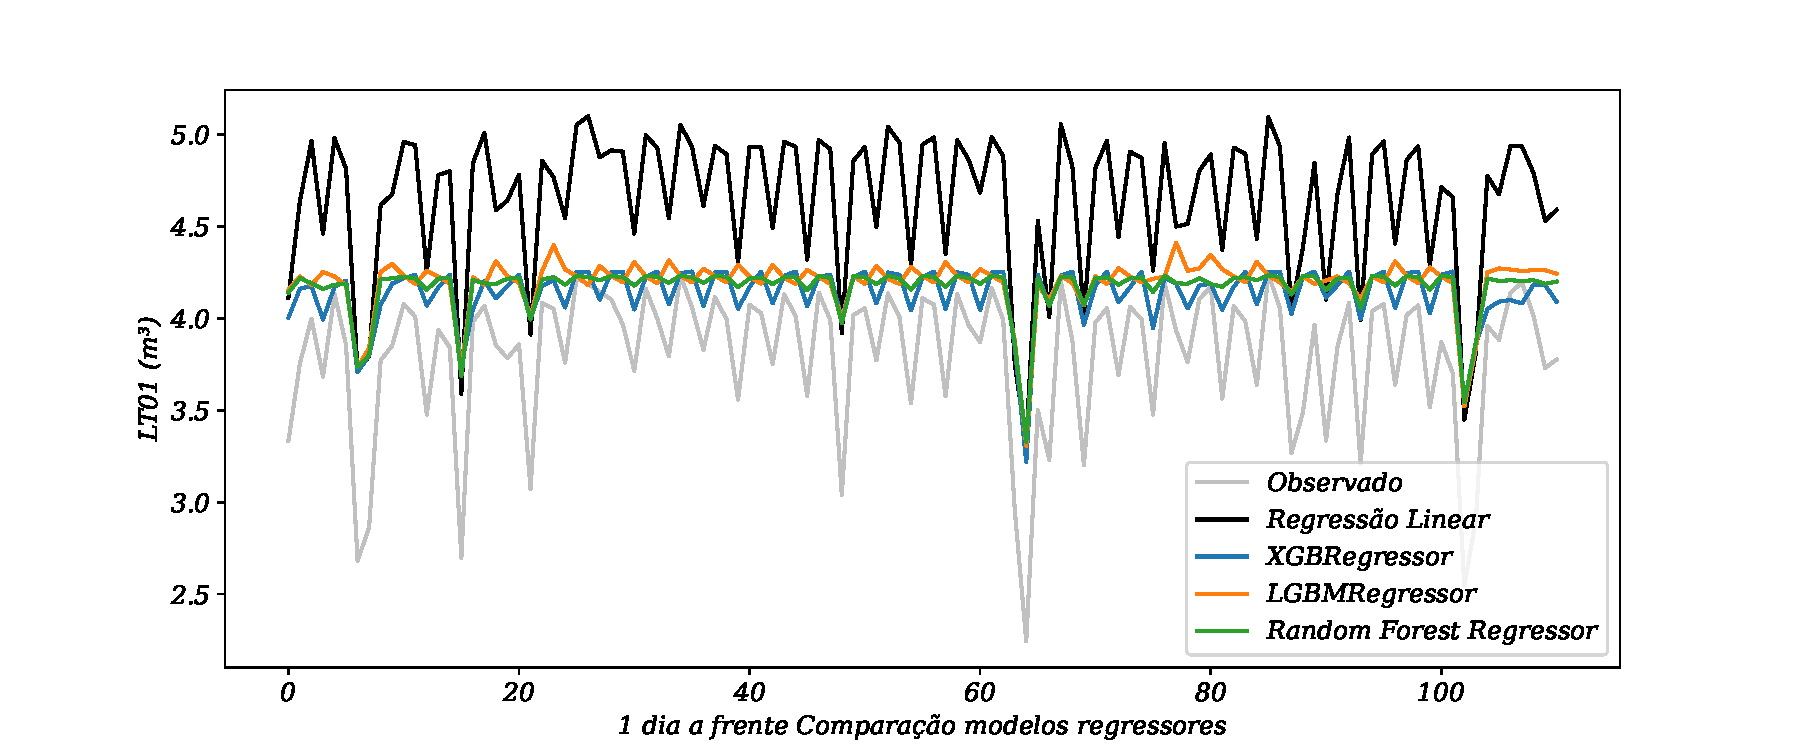
\includegraphics[width=1\linewidth]{Apendices/Figuras/modelagem-24h/1-LR-XGB-LGBM-RF}
	
	Fonte: Autoria própria.
\end{figure}

\begin{figure}[H]
	\centering
	\caption{Comparação dos modelos Regressão linear, XGB Regressão, Ligth GBM Regressão e Regressão de Floresta Aleatória, 7 dias a frente }
	\label{fig:10-LR-XGB-LGBM-RF24}
	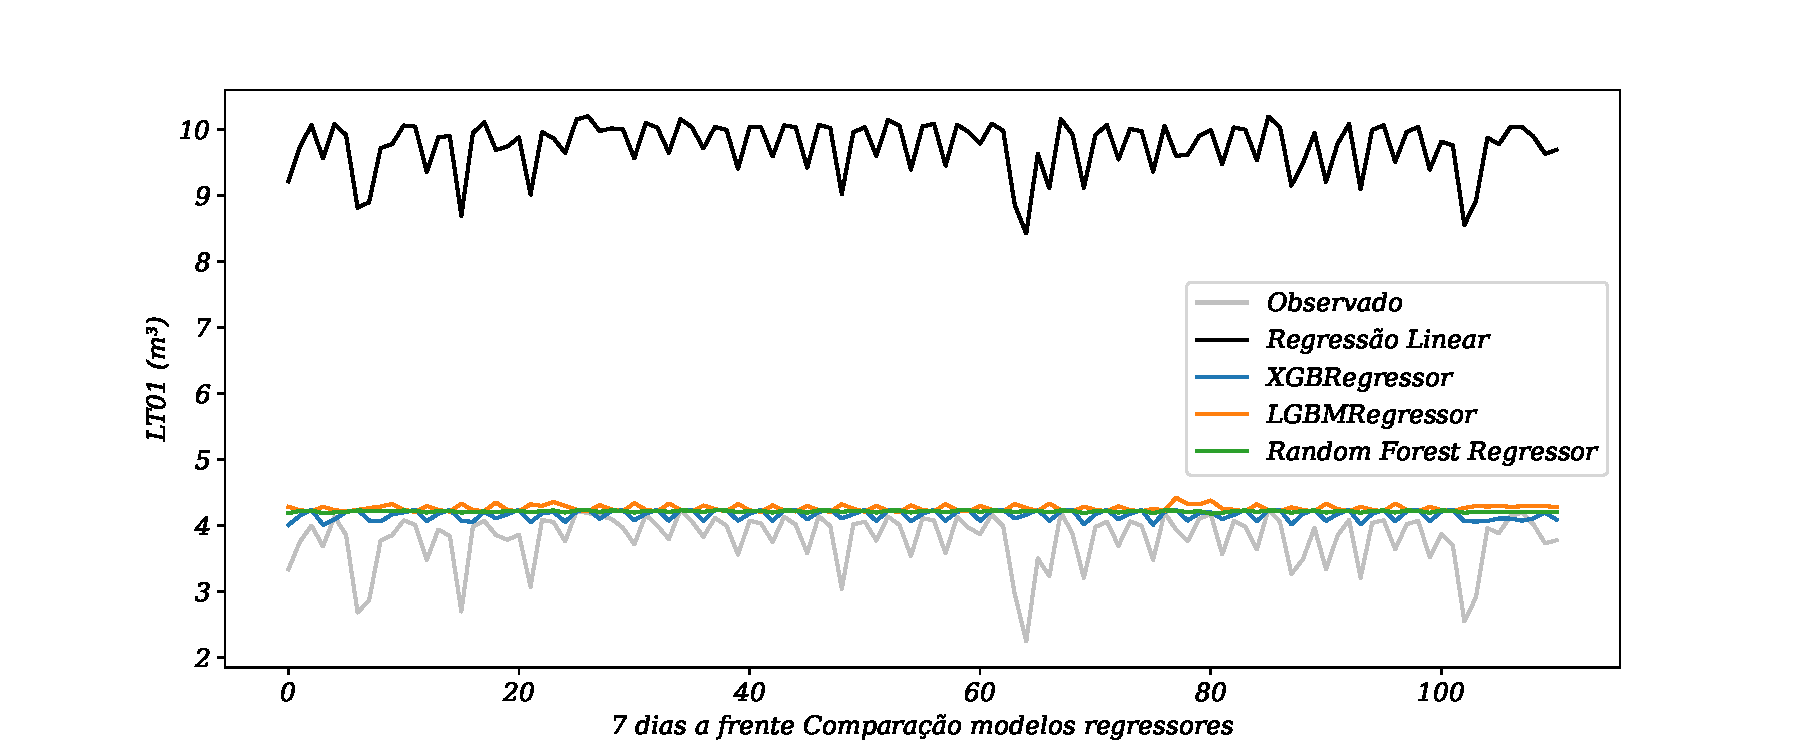
\includegraphics[width=1\linewidth]{Apendices/Figuras/modelagem-24h/7-LR-XGB-LGBM-RF}
	
	Fonte: Autoria própria.
\end{figure}


\begin{figure}[H]
	\centering
	\caption{Comparação dos modelos Regressão linear, XGB Regressão, Ligth GBM Regressão e Regressão de Floresta Aleatória, 14 dias a frente }
	\label{fig:30-LR-XGB-LGBM-RF24}
	\includegraphics[width=1\linewidth]{Apendices/Figuras/modelagem-24h/14-LR-XGB-LGBM-RF}
	
	Fonte: Autoria própria.
\end{figure}

\begin{figure}[H]
	\centering
	\caption{Comparação dos modelos Regressão linear, XGB Regressão, Ligth GBM Regressão e Regressão de Floresta Aleatória, 30 dias a frente }
	\label{fig:60-LR-XGB-LGBM-RF24}
	\includegraphics[width=1\linewidth]{Apendices/Figuras/modelagem-24h/30-LR-XGB-LGBM-RF}
	
	Fonte: Autoria própria.
\end{figure}


%-----------------------------------------------------------------
%% FIM DO DOCUMENTO
\printnomenclature

\end{document}